\documentclass[12pt,a4paper]{article}
% ================================================================
%  PRÉAMBULE COMMUN - ANNALES CORRIGÉES
%  Université de Kara - FaST - Licence Fondamentale MPC
%  Design optimisé impression noir et blanc
% ================================================================

% -- ENCODAGE & LANGUE --
\usepackage[utf8]{inputenc}
\usepackage[T1]{fontenc}
\usepackage[french]{babel}
\usepackage{lmodern}
\usepackage{microtype}

% -- MISE EN PAGE --
\usepackage[a4paper, top=2.8cm, bottom=2.5cm, left=2.5cm, right=2.5cm, headheight=14pt]{geometry}
\usepackage{setspace}
\setstretch{1.2}
\usepackage{parskip}
\setlength{\parindent}{1.2em}
\setlength{\parskip}{4pt}

% -- MATHS --
\usepackage{amsmath, amssymb, mathtools, amsthm}
\usepackage{mathrsfs}
\usepackage{dsfont}
\usepackage{bm}
\usepackage{cancel}
\usepackage{textcomp}
% Définition de \oiint (intégrale de surface fermée) sans package supplémentaire
\newcommand{\oiint}{\mathop{\iint\!\!\!\!\!\!\!\bigcirc}\limits}

% -- PHYSIQUE & CHIMIE --
\usepackage{physics}
\usepackage{siunitx}
% Lorsque physics est chargé, siunitx omet \qty. On le restaure ici :
\AtBeginDocument{\RenewCommandCopy\qty\SI}
\sisetup{locale = FR, detect-all, output-decimal-marker={,}}
% Commande de substitution pour les unités posant problème avec pdflatex
% (ohm, degreeCelsius, micro, angstrom, percent utilisent des caractères non-ASCII)
\newcommand{\qtyohm}[1]{\ensuremath{\num{#1}\,\Omega}}
\newcommand{\qtydegc}[1]{\ensuremath{\num{#1}\,{}^\circ\text{C}}}
\newcommand{\qtyangstrom}[1]{\ensuremath{\num{#1}\,\text{\AA}}}
\newcommand{\qtypercent}[1]{\ensuremath{\num{#1}\,\%}}
\newcommand{\qtyum}[1]{\ensuremath{\num{#1}\,\mu\text{m}}}
\usepackage[version=4]{mhchem}

% -- GRAPHISMES --
\usepackage{graphicx}
\usepackage{float}
\usepackage{caption}
\usepackage{subcaption}
\usepackage{wrapfig}
\usepackage{tikz}
\usetikzlibrary{calc, arrows.meta, patterns, shapes.geometric}
\usepackage{pgfplots}
\pgfplotsset{compat=1.18}

% -- TABLEAUX --
\usepackage{booktabs}
\usepackage{array}
\usepackage{tabularx}
\usepackage{multirow}

% -- LISTES --
\usepackage{enumitem}
\setlist[enumerate]{topsep=3pt, itemsep=2pt, parsep=0pt}
\setlist[itemize]{topsep=3pt, itemsep=2pt, parsep=0pt, label={.}}

% -- BOÎTES (noir et blanc) --
\usepackage{mdframed}
\usepackage{tcolorbox}
\tcbuselibrary{skins, breakable, theorems}

% Boîte EXERCICE : encadré avec filet épais, fond blanc
\newmdenv[
  linewidth=1.2pt,
  linecolor=black,
  roundcorner=3pt,
  skipabove=10pt,
  skipbelow=6pt,
  innertopmargin=8pt,
  innerbottommargin=8pt,
  innerleftmargin=10pt,
  innerrightmargin=10pt,
  backgroundcolor=white,
  frametitle={\bfseries\small Exercice},
  frametitlealignment=\raggedright,
  frametitleaboveskip=4pt,
  frametitlebelowskip=4pt,
]{boiteexercice}

% Boîte CORRIGÉ : fond gris très clair + filet fin
\newmdenv[
  linewidth=0.6pt,
  linecolor=black,
  leftline=true,
  rightline=false,
  topline=false,
  bottomline=false,
  linecolor=black,
  innerleftmargin=12pt,
  innerrightmargin=8pt,
  innertopmargin=6pt,
  innerbottommargin=6pt,
  backgroundcolor=gray!8,
  skipabove=4pt,
  skipbelow=8pt,
]{boitecorrige}

% Boîte RÉSUMÉ DE COURS : double encadré
\newmdenv[
  linewidth=0.8pt,
  linecolor=black,
  roundcorner=2pt,
  backgroundcolor=gray!12,
  innertopmargin=10pt,
  innerbottommargin=10pt,
  innerleftmargin=12pt,
  innerrightmargin=12pt,
  skipabove=12pt,
  skipbelow=8pt,
]{boiteresume}

% Boîte ATTENTION/REMARQUE : barre gauche épaisse
\newmdenv[
  leftline=true,
  rightline=false,
  topline=false,
  bottomline=false,
  linewidth=3pt,
  linecolor=black,
  backgroundcolor=gray!5,
  innerleftmargin=12pt,
  innerrightmargin=8pt,
  innertopmargin=5pt,
  innerbottommargin=5pt,
  skipabove=6pt,
  skipbelow=6pt,
]{boiteremarque}

% -- DIFFICULTÉ DES EXERCICES --
\newcommand{\facile}{$\star$}
\newcommand{\moyen}{$\star\!\star$}
\newcommand{\difficile}{$\star\!\star\!\star$}
\newcommand{\niveau}[1]{\hfill\textbf{#1}\hspace{2pt}}

% -- EN-TÊTES ET PIEDS DE PAGE --
\usepackage{fancyhdr}
\pagestyle{fancy}
\fancyhf{}
\renewcommand{\headrulewidth}{0.5pt}
\renewcommand{\footrulewidth}{0.3pt}

% -- HYPERLIENS --
\usepackage[hidelinks]{hyperref}
\hypersetup{
    colorlinks=false,
    pdftitle={Annale Corrigée - Licence MPC - Université de Kara}
}

% -- TITRES --
\usepackage{titlesec}
\titleformat{\section}{\Large\bfseries}{\thesection.}{0.8em}{}[\vspace{2pt}\hrule\vspace{4pt}]
\titleformat{\subsection}{\large\bfseries}{\thesubsection.}{0.7em}{}
\titleformat{\subsubsection}{\normalsize\bfseries}{\thesubsubsection.}{0.6em}{}

% -- THÉORÈMES --
\theoremstyle{definition}
\newtheorem{defn}{Définition}[section]
\newtheorem{prop}{Propriété}[section]
\newtheorem{thm}{Théorème}[section]
\newtheorem{corol}{Corollaire}[section]
\newtheorem{exemple}{Exemple}[section]

% -- COMMANDES MATHÉMATIQUES UTILES --
\newcommand{\vect}[1]{\overrightarrow{#1}}
\newcommand{\R}{\mathbb{R}}
\newcommand{\N}{\mathbb{N}}
\newcommand{\Z}{\mathbb{Z}}
\newcommand{\C}{\mathbb{C}}
\renewcommand{\d}{\mathrm{d}}
\newcommand{\deriv}[2]{\dfrac{\d #1}{\d #2}}
\newcommand{\dpart}[2]{\dfrac{\partial #1}{\partial #2}}
\newcommand{\rot}{\overrightarrow{\mathrm{rot}}\,}
\renewcommand{\div}{\mathrm{div}\,}
\renewcommand{\grad}{\overrightarrow{\mathrm{grad}}\,}
\newcommand{\e}{\mathrm{e}}
\newcommand{\ii}{\mathrm{i}}
\renewcommand{\Tr}{\mathrm{Tr}}

% Numérotation des équations par section
\numberwithin{equation}{section}

% -- RÉSULTATS ENCADRÉS --
\newcommand{\res}[1]{\[\boxed{#1}\]}

% -- REMARQUE INLINE --
\newcommand{\rmq}[1]{\begin{boiteremarque}\textbf{Remarque.} #1\end{boiteremarque}}

% -- MISE EN VALEUR DU RÉSULTAT FINAL --
\newcommand{\reponse}[1]{%
  \begin{center}
    \fbox{\begin{minipage}{0.92\textwidth}\centering #1\end{minipage}}
  \end{center}%
}

\def\inMainDoc{}

% En-têtes générales de l'annale L1
\lhead{\small\textit{Annale corrigée - Licence 1 - MPC}}
\rhead{\small\textit{FaST, Université de Kara}}
\cfoot{\thepage}

\graphicspath{{images/}}

\usepackage{listings}
\lstset{
  language=C,
  basicstyle=\ttfamily\small,
  keywordstyle=\bfseries,
  commentstyle=\itshape,
  numbers=left,
  numberstyle=\tiny,
  numbersep=8pt,
  frame=single,
  breaklines=true,
  tabsize=4,
  showstringspaces=false
}
\begin{document}

% ================================================================
%  PAGE DE GARDE
% ================================================================
\begin{titlepage}
\centering
\thispagestyle{empty}


\includegraphics[width=0.22\textwidth]{images/logo1.png}\\[0.4cm]
{\large\bfseries UNIVERSITÉ DE KARA}\\[0.1cm]
{\normalsize Faculté des Sciences et Techniques (FaST)}\\[0.1cm]
{\normalsize Département de Physique}\\[0.3cm]
\rule{\textwidth}{1.5pt}\\[0.1cm]
\rule{\textwidth}{0.4pt}\\[0.8cm]

\begin{tikzpicture}
  \draw[line width=2pt] (-7.5,-2.6) rectangle (7.5,2.6);
  \draw[line width=0.6pt] (-7.2,-2.3) rectangle (7.2,2.3);
  \node at (0, 1.2) {\Huge\bfseries ANNALE D'EXERCICES};
  \node at (0, 0.2) {\Huge\bfseries ET EXAMENS CORRIGÉS};
  \node at (0,-0.9) {\large\bfseries Semestres 1 et 2};
  \node at (0,-1.7) {\normalsize Exercices classiques, annales et examens résolus avec méthode};
\end{tikzpicture}

\vspace{0.7cm}
{\LARGE\bfseries LICENCE FONDAMENTALE EN MATHÉMATIQUES, PHYSIQUE ET CHIMIE}\\[0.2cm]
{\Large\bfseries PARCOURS PREMIÈRE ANNÉE (L1)}\\[0.3cm]
\rule{0.6\textwidth}{0.4pt}\\[0.4cm]
{\small\itshape Comme toute \oe{}uvre humaine n'est jamais parfaite, prière de signaler toute erreur ou imprécision constatée dans ce document.}

\vspace{0.7cm}
\rule{\textwidth}{0.4pt}\\[0.5cm]

\begin{flushleft}
{\large\bfseries\underline{AUTEURS}}\\[0.3cm]
\hspace{1cm}{\bfseries DJABON Ounimborbitibou}\\
\hspace{1.5cm}{\itshape Master en Physique Théorique}\\
\hspace{1.5cm}{\itshape Master in Mathematical Sciences, AIMS Ghana}\\[0.25cm]
\hspace{1cm}{\bfseries BOUTCHOKA Malaki}\\
\hspace{1.5cm}{\itshape Master en Matériaux Avancés en Électricité}\\
\hspace{1.5cm}{\itshape Université de Lomé}
\end{flushleft}

\vspace{0.5cm}
\rule{\textwidth}{0.4pt}\\[0.15cm]
{\small Université de Kara, FaST \hfill Octobre 2025}

\end{titlepage}

% ================================================================
%  AVANT-PROPOS
% ================================================================
\newpage
\thispagestyle{plain}
\pagestyle{fancy}

\section*{Avant-propos}

Chères étudiantes, chers étudiants de première année en Mathématiques, Physique et Chimie,

Cet ouvrage a été conçu spécialement pour vous accompagner tout au long de votre parcours universitaire. Il représente bien plus qu'un simple recueil d'exercices et d'examens : il se veut un outil de formation rigoureux, un compagnon de travail fidèle dans votre découverte des sciences fondamentales.

Vous trouverez dans cette annale l'ensemble des Unités d'Enseignement qui constituent le socle de votre première année :

\begin{itemize}
  \item Atomistique
  \item Algèbre linéaire
  \item Analyse vectorielle
  \item Calcul différentiel dans $\mathbb{R}$
  \item Calcul intégral dans $\mathbb{R}$
  \item Électrocinétique et régime variable
  \item Électrostatique et magnétostatique
  \item Logique et algèbre de base
  \item Mécanique du point matériel
  \item Programmation en langage C
  \item Optique géométrique
\end{itemize}

Chaque UE s'articule de la même manière : un \textbf{résumé de cours} condensé rappelle les résultats essentiels à maîtriser, suivi d'exercices progressifs dont le degré de difficulté est indiqué par des étoiles ($\star$ : accessible, $\star\star$ : intermédiaire, $\star\star\star$ : difficile). Chaque exercice est suivi de son corrigé détaillé, rédigé étape par étape.

Pour tirer le meilleur parti de cet outil, nous vous conseillons de :

\begin{enumerate}
  \item \textbf{Revoir d'abord le résumé de cours} avant d'aborder les exercices.
  \item \textbf{Chercher activement} chaque problème avant de consulter la solution.
  \item \textbf{Analyser les méthodes} de résolution plutôt que de simplement recopier.
  \item \textbf{Identifier vos points faibles} pour y remédier efficacement.
\end{enumerate}

Retenez ceci : aucun ouvrage, aussi complet soit-il, ne peut remplacer votre curiosité intellectuelle et votre engagement personnel. Les sciences exactes demandent de la persévérance, de la rigueur et, parfois, beaucoup d'efforts. Mais c'est précisément ce dépassement de soi qui fera de vous des scientifiques accomplis.

\begin{flushright}
\emph{«\,Le génie est fait d'un pour cent d'inspiration et de quatre-vingt-dix-neuf pour cent de transpiration.\,»}\\
\textbf{Thomas Edison}
\end{flushright}

Nous vous souhaitons une excellente utilisation de cette annale et plein succès dans vos études scientifiques.

\vspace{1cm}
\begin{flushright}
\textit{DJABON Ounimborbitibou \& BOUTCHOKA Malaki}
\end{flushright}

% ================================================================
%  TABLE DES MATIÈRES
% ================================================================
\newpage
\tableofcontents
\newpage

% ================================================================
%  UE 1 : ATOMISTIQUE
% ================================================================
\newpage
\thispagestyle{empty}
\begin{tikzpicture}[remember picture, overlay]
  \fill[gray!12] ([xshift=1.5cm, yshift=3cm]current page.south west)
    rectangle ([xshift=-1.5cm, yshift=-3cm]current page.north east);
  \draw[line width=3pt] ([xshift=1.5cm,yshift=-3cm]current page.north west)
    -- ([xshift=-1.5cm,yshift=-3cm]current page.north east);
  \draw[line width=3pt] ([xshift=1.5cm,yshift=3cm]current page.south west)
    -- ([xshift=-1.5cm,yshift=3cm]current page.south east);
  \node[align=center] at (current page.center) {%
    {\fontsize{36}{44}\bfseries\selectfont ATOMISTIQUE}\\[1.2cm]
    {\large\itshape Structure de l'atome - Modèle de Bohr}\\[0.4cm]
    {\large\itshape Configurations électroniques}\\[1.8cm]
    {\normalsize Licence 1 - UE 1}
  };
  \node[anchor=south west] at ([xshift=2cm,yshift=2cm]current page.south west)
    {\large\bfseries UE 1};
\end{tikzpicture}
\newpage

\addcontentsline{toc}{section}{ATOMISTIQUE}
\ifdefined\inMainDoc\else
\documentclass[12pt,a4paper]{article}
% ================================================================
%  PRÉAMBULE COMMUN - ANNALES CORRIGÉES
%  Université de Kara - FaST - Licence Fondamentale MPC
%  Design optimisé impression noir et blanc
% ================================================================

% -- ENCODAGE & LANGUE --
\usepackage[utf8]{inputenc}
\usepackage[T1]{fontenc}
\usepackage[french]{babel}
\usepackage{lmodern}
\usepackage{microtype}

% -- MISE EN PAGE --
\usepackage[a4paper, top=2.8cm, bottom=2.5cm, left=2.5cm, right=2.5cm, headheight=14pt]{geometry}
\usepackage{setspace}
\setstretch{1.2}
\usepackage{parskip}
\setlength{\parindent}{1.2em}
\setlength{\parskip}{4pt}

% -- MATHS --
\usepackage{amsmath, amssymb, mathtools, amsthm}
\usepackage{mathrsfs}
\usepackage{dsfont}
\usepackage{bm}
\usepackage{cancel}
\usepackage{textcomp}
% Définition de \oiint (intégrale de surface fermée) sans package supplémentaire
\newcommand{\oiint}{\mathop{\iint\!\!\!\!\!\!\!\bigcirc}\limits}

% -- PHYSIQUE & CHIMIE --
\usepackage{physics}
\usepackage{siunitx}
% Lorsque physics est chargé, siunitx omet \qty. On le restaure ici :
\AtBeginDocument{\RenewCommandCopy\qty\SI}
\sisetup{locale = FR, detect-all, output-decimal-marker={,}}
% Commande de substitution pour les unités posant problème avec pdflatex
% (ohm, degreeCelsius, micro, angstrom, percent utilisent des caractères non-ASCII)
\newcommand{\qtyohm}[1]{\ensuremath{\num{#1}\,\Omega}}
\newcommand{\qtydegc}[1]{\ensuremath{\num{#1}\,{}^\circ\text{C}}}
\newcommand{\qtyangstrom}[1]{\ensuremath{\num{#1}\,\text{\AA}}}
\newcommand{\qtypercent}[1]{\ensuremath{\num{#1}\,\%}}
\newcommand{\qtyum}[1]{\ensuremath{\num{#1}\,\mu\text{m}}}
\usepackage[version=4]{mhchem}

% -- GRAPHISMES --
\usepackage{graphicx}
\usepackage{float}
\usepackage{caption}
\usepackage{subcaption}
\usepackage{wrapfig}
\usepackage{tikz}
\usetikzlibrary{calc, arrows.meta, patterns, shapes.geometric}
\usepackage{pgfplots}
\pgfplotsset{compat=1.18}

% -- TABLEAUX --
\usepackage{booktabs}
\usepackage{array}
\usepackage{tabularx}
\usepackage{multirow}

% -- LISTES --
\usepackage{enumitem}
\setlist[enumerate]{topsep=3pt, itemsep=2pt, parsep=0pt}
\setlist[itemize]{topsep=3pt, itemsep=2pt, parsep=0pt, label={.}}

% -- BOÎTES (noir et blanc) --
\usepackage{mdframed}
\usepackage{tcolorbox}
\tcbuselibrary{skins, breakable, theorems}

% Boîte EXERCICE : encadré avec filet épais, fond blanc
\newmdenv[
  linewidth=1.2pt,
  linecolor=black,
  roundcorner=3pt,
  skipabove=10pt,
  skipbelow=6pt,
  innertopmargin=8pt,
  innerbottommargin=8pt,
  innerleftmargin=10pt,
  innerrightmargin=10pt,
  backgroundcolor=white,
  frametitle={\bfseries\small Exercice},
  frametitlealignment=\raggedright,
  frametitleaboveskip=4pt,
  frametitlebelowskip=4pt,
]{boiteexercice}

% Boîte CORRIGÉ : fond gris très clair + filet fin
\newmdenv[
  linewidth=0.6pt,
  linecolor=black,
  leftline=true,
  rightline=false,
  topline=false,
  bottomline=false,
  linecolor=black,
  innerleftmargin=12pt,
  innerrightmargin=8pt,
  innertopmargin=6pt,
  innerbottommargin=6pt,
  backgroundcolor=gray!8,
  skipabove=4pt,
  skipbelow=8pt,
]{boitecorrige}

% Boîte RÉSUMÉ DE COURS : double encadré
\newmdenv[
  linewidth=0.8pt,
  linecolor=black,
  roundcorner=2pt,
  backgroundcolor=gray!12,
  innertopmargin=10pt,
  innerbottommargin=10pt,
  innerleftmargin=12pt,
  innerrightmargin=12pt,
  skipabove=12pt,
  skipbelow=8pt,
]{boiteresume}

% Boîte ATTENTION/REMARQUE : barre gauche épaisse
\newmdenv[
  leftline=true,
  rightline=false,
  topline=false,
  bottomline=false,
  linewidth=3pt,
  linecolor=black,
  backgroundcolor=gray!5,
  innerleftmargin=12pt,
  innerrightmargin=8pt,
  innertopmargin=5pt,
  innerbottommargin=5pt,
  skipabove=6pt,
  skipbelow=6pt,
]{boiteremarque}

% -- DIFFICULTÉ DES EXERCICES --
\newcommand{\facile}{$\star$}
\newcommand{\moyen}{$\star\!\star$}
\newcommand{\difficile}{$\star\!\star\!\star$}
\newcommand{\niveau}[1]{\hfill\textbf{#1}\hspace{2pt}}

% -- EN-TÊTES ET PIEDS DE PAGE --
\usepackage{fancyhdr}
\pagestyle{fancy}
\fancyhf{}
\renewcommand{\headrulewidth}{0.5pt}
\renewcommand{\footrulewidth}{0.3pt}

% -- HYPERLIENS --
\usepackage[hidelinks]{hyperref}
\hypersetup{
    colorlinks=false,
    pdftitle={Annale Corrigée - Licence MPC - Université de Kara}
}

% -- TITRES --
\usepackage{titlesec}
\titleformat{\section}{\Large\bfseries}{\thesection.}{0.8em}{}[\vspace{2pt}\hrule\vspace{4pt}]
\titleformat{\subsection}{\large\bfseries}{\thesubsection.}{0.7em}{}
\titleformat{\subsubsection}{\normalsize\bfseries}{\thesubsubsection.}{0.6em}{}

% -- THÉORÈMES --
\theoremstyle{definition}
\newtheorem{defn}{Définition}[section]
\newtheorem{prop}{Propriété}[section]
\newtheorem{thm}{Théorème}[section]
\newtheorem{corol}{Corollaire}[section]
\newtheorem{exemple}{Exemple}[section]

% -- COMMANDES MATHÉMATIQUES UTILES --
\newcommand{\vect}[1]{\overrightarrow{#1}}
\newcommand{\R}{\mathbb{R}}
\newcommand{\N}{\mathbb{N}}
\newcommand{\Z}{\mathbb{Z}}
\newcommand{\C}{\mathbb{C}}
\renewcommand{\d}{\mathrm{d}}
\newcommand{\deriv}[2]{\dfrac{\d #1}{\d #2}}
\newcommand{\dpart}[2]{\dfrac{\partial #1}{\partial #2}}
\newcommand{\rot}{\overrightarrow{\mathrm{rot}}\,}
\renewcommand{\div}{\mathrm{div}\,}
\renewcommand{\grad}{\overrightarrow{\mathrm{grad}}\,}
\newcommand{\e}{\mathrm{e}}
\newcommand{\ii}{\mathrm{i}}
\renewcommand{\Tr}{\mathrm{Tr}}

% Numérotation des équations par section
\numberwithin{equation}{section}

% -- RÉSULTATS ENCADRÉS --
\newcommand{\res}[1]{\[\boxed{#1}\]}

% -- REMARQUE INLINE --
\newcommand{\rmq}[1]{\begin{boiteremarque}\textbf{Remarque.} #1\end{boiteremarque}}

% -- MISE EN VALEUR DU RÉSULTAT FINAL --
\newcommand{\reponse}[1]{%
  \begin{center}
    \fbox{\begin{minipage}{0.92\textwidth}\centering #1\end{minipage}}
  \end{center}%
}


% En-têtes spécifiques à ce fichier
\lhead{\small\textit{Atomistique - Licence 1}}
\rhead{\small\textit{FaST, Université de Kara}}
\cfoot{\thepage}

\begin{document}
\fi

\begin{center}
  {\LARGE\bfseries ATOMISTIQUE}\\[0.3cm]
  {\normalsize Licence 1 - Mathématiques, Physique et Chimie}\\[0.1cm]
  \rule{0.7\textwidth}{0.8pt}
\end{center}

\vspace{0.3cm}

% ================================================================
\section*{Résumé du cours}
% ================================================================

\begin{boiteresume}

\textbf{1. Le modèle de Bohr.} L'atome d'hydrogène est formé d'un proton et d'un électron gravitant sur une orbite circulaire de rang $n$ (nombre quantique principal, $n \in \mathbb{N}^*$). Les hypothèses de Bohr imposent la quantification du moment cinétique orbital : $L = m_e v r = n\hbar$, avec $\hbar = h/(2\pi)$.

Le rayon de l'orbite de rang $n$ et l'énergie associée pour un atome hydrogénoïde de numéro atomique $Z$ sont :
\[
r_n = \frac{n^2}{Z}\,a_0 \qquad \text{avec} \qquad a_0 = \frac{\varepsilon_0 h^2}{\pi m_e e^2} \approx \qtyangstrom{0.529}
\]
\[
E_n = -\frac{Z^2}{n^2}\,E_1^{(H)} \qquad \text{avec} \qquad E_1^{(H)} = \qty{-13.6}{eV}
\]

\textbf{2. Configurations électroniques.} Le remplissage des sous-couches obéit à trois règles :
\begin{itemize}[nosep]
  \item \textbf{Règle de Klechkowski} : remplissage dans l'ordre croissant de $n+\ell$, puis par $n$ croissant en cas d'égalité. Ordre pratique : 1s, 2s, 2p, 3s, 3p, 4s, 3d, 4p, 5s, 4d, \dots
  \item \textbf{Règle de Pauli} : deux électrons d'une même case ont nécessairement des spins antiparallèles ; aucune case ne peut contenir plus de deux électrons.
  \item \textbf{Règle de Hund} : à sous-couche partiellement remplie, les électrons occupent d'abord chacun une case différente, avec des spins parallèles.
\end{itemize}

\textbf{3. Orbitales moléculaires (OM).} La combinaison linéaire d'orbitales atomiques (CLOA) donne des OM liantes ($\sigma$, $\pi$) et antiliantes ($\sigma^*$, $\pi^*$). L'ordre de remplissage pour les molécules homodiatomiques de la 2\textsuperscript{e} période est :
$\sigma_{1s} < \sigma^*_{1s} < \sigma_{2s} < \sigma^*_{2s} < (\pi_{2p_x}, \pi_{2p_y}) < \sigma_{2p_z} < \dots$

L'indice de liaison vaut : $\omega = \dfrac{N_l - N_{al}}{2}$, où $N_l$ est le nombre d'électrons liants et $N_{al}$ le nombre d'antiliants.

\textbf{4. Transition énergétique et longueur d'onde.} L'énergie d'un photon émis ou absorbé lors d'une transition $n_i \to n_f$ est :
\[
\Delta E = E_{n_f} - E_{n_i} = h\nu = \frac{hc}{\lambda}
\]
Si $\Delta E < 0$ : émission ; si $\Delta E > 0$ : absorption.

\end{boiteresume}

\newpage

% ================================================================
\section{Modèle de Bohr et atomes hydrogénoïdes}
% ================================================================

\subsection*{Exercice 1 - Isotopes du carbone et masse atomique de l'azote \niveau{\facile}}

\begin{boiteexercice}
Un atome de carbone de masse atomique 12 possède un isotope de masse atomique 14. L'azote naturel est composé de deux isotopes : $^{14}_{7}$N (abondance \qtypercent{99.635}) et $^{15}_{7}$N (abondance \qtypercent{0.365}), de masses atomiques respectives \qty{14.007515}{u} et \qty{15.004863}{u}.

\begin{enumerate}
  \item Définir isotope et donner le nombre de neutrons de chaque isotope du carbone.
  \item Calculer la masse atomique moyenne de l'azote naturel.
\end{enumerate}
\end{boiteexercice}

\begin{boitecorrige}
\textbf{1.} Deux isotopes d'un même élément ont le même numéro atomique $Z$ mais des nombres de masse $A$ différents (donc des nombres de neutrons $N = A - Z$ différents).

Pour le carbone ($Z = 6$) : $^{12}_{6}$C possède $12 - 6 = 6$ neutrons ; $^{14}_{6}$C en possède $14 - 6 = 8$.

\textbf{2.} La masse atomique moyenne de l'azote naturel est la moyenne pondérée par les abondances isotopiques :
\[
\overline{M} = \frac{99{,}635}{100} \times 14{,}007515 + \frac{0{,}365}{100} \times 15{,}004863
\]
\[
\overline{M} = 13{,}9704 + 0{,}0548 \approx \qty{14.01}{g.mol^{-1}}
\]
\end{boitecorrige}

\begin{center}
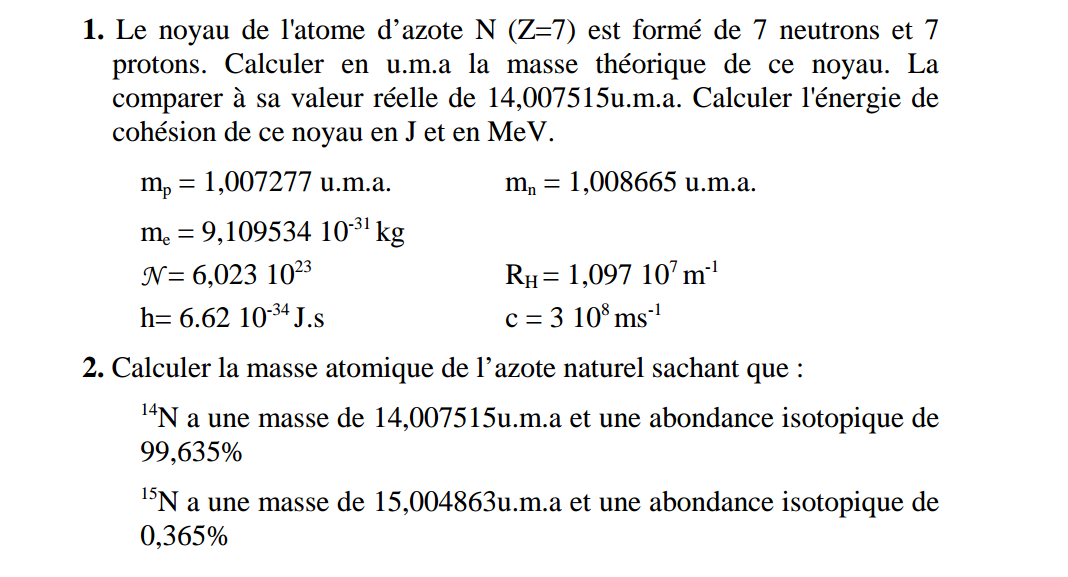
\includegraphics[width=0.6\textwidth]{images/atomistique/atom-001-000.png}
\captionof{figure}{\small Isotopes du carbone : $^{12}_6\text{C}$ et $^{14}_6\text{C}$, même $Z=6$, $A$ différents.}
\end{center}
\begin{center}

\includegraphics[width=0.6\textwidth]{images/atomistique/atom-001-001.png}
\captionof{figure}{\small Isotopes de l'azote : $^{14}_7\text{N}$ (majoritaire) et $^{15}_7\text{N}$ (trace).}
\end{center}
\begin{center}
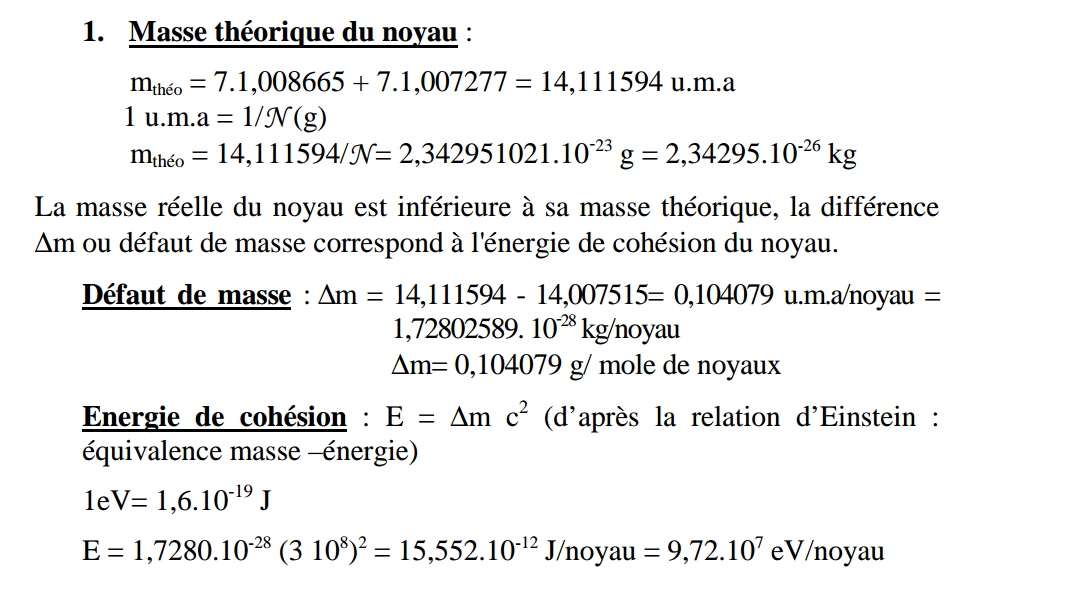
\includegraphics[width=0.6\textwidth]{images/atomistique/atom-001-002.png}
\captionof{figure}{\small Composition du noyau : protons et neutrons des isotopes de l'azote.}
\end{center}
\begin{center}

\includegraphics[width=0.6\textwidth]{images/atomistique/atom-001-003.png}
\captionof{figure}{\small Calcul de la masse atomique moyenne par pondération des abondances.}
\end{center}

\subsection*{Exercice 2 - Atome hydrogénoïde : modèle de Bohr \niveau{\moyen}}

\begin{boiteexercice}
Pour un atome hydrogénoïde (noyau de charge $+Ze$ autour duquel gravite un électron) :

\begin{enumerate}
  \item Établir les formules donnant :
    \begin{enumerate}[label=(\alph*)]
      \item le rayon $r_n$ de l'orbite de rang $n$,
      \item l'énergie totale $E_n$ du système noyau-électron,
      \item les expressions de $r_n$ et $E_n$ en fonction des grandeurs correspondantes de l'hydrogène.
    \end{enumerate}
  \item Calculer en eV et en joules les énergies des quatre premiers niveaux de l'ion $\text{Li}^{2+}$.
  \item Quelle énergie doit absorber un ion $\text{Li}^{2+}$ pour que l'électron passe du niveau fondamental au premier niveau excité ?
  \item Si cette énergie est fournie sous forme lumineuse, calculer la longueur d'onde $\lambda$ du rayonnement correspondant.
\end{enumerate}

\textbf{Données :} $\text{Li}(Z=3)$, $1\,\text{eV} = \qty{1.6e-19}{J}$, $c = \qty{3e8}{m.s^{-1}}$, $h = \qty{6.62e-34}{J.s}$.
\end{boiteexercice}

\begin{boitecorrige}
\textbf{1.(a) Rayon de l'orbite.}

L'électron est en équilibre entre la force électrostatique et la force centrifuge :
\[
\frac{Ze^2}{4\pi\varepsilon_0 r^2} = \frac{m_e v^2}{r} \tag{1}
\]
La quantification de Bohr impose $m_e v r = n\hbar$, soit :
\[
v = \frac{n\hbar}{m_e r} \tag{2}
\]
En substituant (2) dans (1) :
\[
\boxed{r_n = \frac{n^2}{Z}\cdot\frac{\varepsilon_0 h^2}{\pi m_e e^2} = \frac{n^2}{Z}\,a_0}
\]

\textbf{1.(b) Énergie totale.}

L'énergie cinétique $E_c = \frac{1}{2}m_e v^2$ et l'énergie potentielle $E_p = -\frac{Ze^2}{4\pi\varepsilon_0 r}$. La condition d'équilibre (1) donne $E_c = -\frac{1}{2}E_p$, d'où $E_t = E_c + E_p = \frac{1}{2}E_p$ :
\[
\boxed{E_n = -\frac{Z^2}{n^2}\cdot\frac{m_e e^4}{8\varepsilon_0^2 h^2} = -\frac{Z^2}{n^2}\,E_1^{(H)}}
\]

\textbf{1.(c) Expressions relatives à l'hydrogène.}

Pour $Z=1$, $n=1$ : $a_0 = (r_1)_H \approx \qtyangstrom{0.529}$ et $E_1^{(H)} = -\qty{13.6}{eV}$. Ainsi :
\[
r_n = \frac{n^2}{Z}\,(r_1)_H \qquad \text{et} \qquad E_n = -\frac{Z^2}{n^2}\times\qty{13.6}{eV}
\]

\textbf{2. Niveaux d'énergie de Li$^{2+}$ ($Z=3$).}

$(E_1)_{\text{Li}^{2+}} = -Z^2 \times \qty{13.6}{eV} = -9 \times \qty{13.6}{eV} = \qty{-122.4}{eV}$

\begin{center}
\begin{tabular}{ccc}
\toprule
$n$ & $E_n$ (eV) & $E_n$ (J) \\
\midrule
1 & $-122{,}4$ & $\qty{-1.96e-17}{}$ \\
2 & $-30{,}6$ & $\qty{-4.90e-18}{}$ \\
3 & $-13{,}6$ & $\qty{-2.18e-18}{}$ \\
4 & $-7{,}65$ & $\qty{-1.22e-18}{}$ \\
\bottomrule
\end{tabular}
\end{center}

\textbf{3. Énergie à absorber pour la transition $n=1 \to n=2$.}

\[
\Delta E = E_2 - E_1 = -30{,}6 - (-122{,}4) = \qty{91.8}{eV} = \qty{1.47e-17}{J}
\]

\textbf{4. Longueur d'onde correspondante.}

\[
\lambda = \frac{hc}{\Delta E} = \frac{6{,}62\times10^{-34}\times3\times10^8}{1{,}47\times10^{-17}} \approx \qty{13.5}{nm}
\]
Ce rayonnement est dans le domaine ultraviolet lointain.
\end{boitecorrige}

\begin{center}
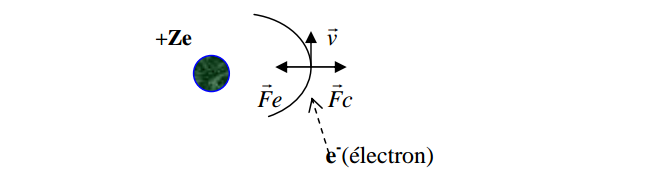
\includegraphics[width=0.55\textwidth]{images/atomistique/atom-002-004.png}
\captionof{figure}{\small Modèle de Bohr de l'atome d'hydrogène : orbites circulaires quantifiées de rayon $r_n = n^2 a_0/Z$.}
\end{center}
\begin{center}

\includegraphics[width=0.55\textwidth]{images/atomistique/atom-002-005.png}
\captionof{figure}{\small Niveaux d'énergie $E_n = -Z^2 E_1^{(H)}/n^2$ de l'ion hydrogénoïde $\text{Li}^{2+}$ ($Z=3$).}
\end{center}

\subsection*{Exercice 3 - Transitions énergétiques de l'atome d'hydrogène \niveau{\moyen}}

\begin{boiteexercice}
\begin{enumerate}
  \item Un atome d'hydrogène initialement à l'état fondamental absorbe \qty{10.2}{eV}. À quel niveau se retrouve l'électron ?
  \item L'électron d'un atome d'hydrogène initialement au niveau $n=3$ émet un rayonnement de longueur d'onde $\lambda = \qtyangstrom{1027}$. À quel niveau se retrouve l'électron ?
\end{enumerate}
\end{boiteexercice}

\begin{boitecorrige}
\textbf{1.} L'énergie absorbée depuis l'état fondamental ($n_i = 1$) est :
\[
\Delta E = E_{n_f} - E_1 = \qty{-13.6}{eV}\left(\frac{1}{n_f^2} - 1\right) = \qty{10.2}{eV}
\]
\[
\frac{1}{n_f^2} = 1 - \frac{10{,}2}{13{,}6} = 0{,}25 \quad \Rightarrow \quad n_f = 2
\]
L'électron se retrouve au niveau $n = 2$.

\textbf{2.} L'énergie emportée par le photon émis est :
\[
|\Delta E| = \frac{hc}{\lambda} = \frac{6{,}62\times10^{-34}\times3\times10^8}{1027\times10^{-10}} = \qty{1.934e-18}{J} = \qty{12.09}{eV}
\]
Depuis $n_i = 3$ :
\[
\Delta E = E_{n_f} - E_3 = \qty{-13.6}{eV}\left(\frac{1}{n_f^2} - \frac{1}{9}\right) = -\qty{12.09}{eV}
\]
\[
\frac{1}{n_f^2} = \frac{1}{9} - \frac{12{,}09}{13{,}6} \approx \frac{1}{9} - 0{,}889 \approx -0{,}778
\]

Cela ne donne pas de solution positive. Revoyons le calcul : l'émission signifie $E_{n_f} < E_{n_i} = E_3 = \qty{-1.51}{eV}$. La condition est :
\[
\frac{1}{n_f^2} - \frac{1}{9} = \frac{|\Delta E|}{13{,}6} \approx 0{,}889
\]
\[
\frac{1}{n_f^2} = \frac{1}{9} + \frac{12{,}09}{13{,}6} = 0{,}111 + 0{,}889 = 1 \quad \Rightarrow \quad n_f = 1
\]
L'électron retombe au niveau fondamental ($n = 1$).
\end{boitecorrige}

\subsection*{Exercice 4 - Niveaux d'énergie et transitions de l'hydrogène \niveau{\moyen}}

\begin{boiteexercice}
Les niveaux d'énergie de l'atome d'hydrogène sont donnés par $E_n = -\dfrac{13{,}6}{n^2}$ (en eV).

\begin{enumerate}
  \item Calculer les énergies des 4 premiers niveaux.
  \item Quel est le niveau fondamental ?
  \item Considérer la transition $n=3 \to n=2$.
    \begin{enumerate}[label=(\alph*)]
      \item S'agit-il d'une émission ou d'une absorption ?
      \item Calculer la longueur d'onde correspondante.
      \item À quel domaine appartient ce rayonnement ?
    \end{enumerate}
  \item L'atome absorbe un photon de $\lambda = \qty{121.7}{nm}$. Quelle transition entraîne cette absorption ?
\end{enumerate}

\textbf{Données :} $h = \qty{6.62e-34}{J.s}$, $c = \qty{3.00e8}{m.s^{-1}}$, $\qty{1}{eV} = \qty{1.60e-19}{J}$.
\end{boiteexercice}

\begin{boitecorrige}
\textbf{1.} $E_1 = \qty{-13.6}{eV}$, $E_2 = \qty{-3.40}{eV}$, $E_3 = \qty{-1.51}{eV}$, $E_4 = \qty{-0.85}{eV}$.

\textbf{2.} Le niveau fondamental est $E_1 = \qty{-13.6}{eV}$ (niveau le plus bas, $n=1$).

\textbf{3.(a)} La transition $n=3 \to n=2$ correspond à $\Delta E = E_2 - E_3 = -3{,}40 - (-1{,}51) = \qty{-1.89}{eV}$. Comme $\Delta E < 0$, il s'agit d'une \textbf{émission}.

\textbf{3.(b)}
\[
|\Delta E| = \qty{1.89}{eV} = 1{,}89 \times 1{,}60\times10^{-19} = \qty{3.02e-19}{J}
\]
\[
\lambda = \frac{hc}{|\Delta E|} = \frac{6{,}62\times10^{-34}\times3{,}00\times10^8}{3{,}02\times10^{-19}} \approx \qty{657}{nm}
\]

\textbf{3.(c)} $\lambda \approx \qty{657}{nm}$ : rayonnement \textbf{rouge} du domaine visible (raie $H_\alpha$ de la série de Balmer).

\textbf{4.} Énergie du photon absorbé :
\[
\Delta E = \frac{hc}{\lambda} = \frac{6{,}62\times10^{-34}\times3{,}00\times10^8}{121{,}7\times10^{-9}} = \qty{1.63e-18}{J} = \qty{10.2}{eV}
\]
La seule transition qui correspond est $n=1 \to n=2$ : $\Delta E = E_2 - E_1 = -3{,}40 + 13{,}6 = \qty{10.2}{eV}$. \\
L'électron passe du niveau fondamental ($n=1$) au premier niveau excité ($n=2$). C'est la raie $\text{Ly}_\alpha$ de la série de Lyman (UV).
\end{boitecorrige}

\begin{center}
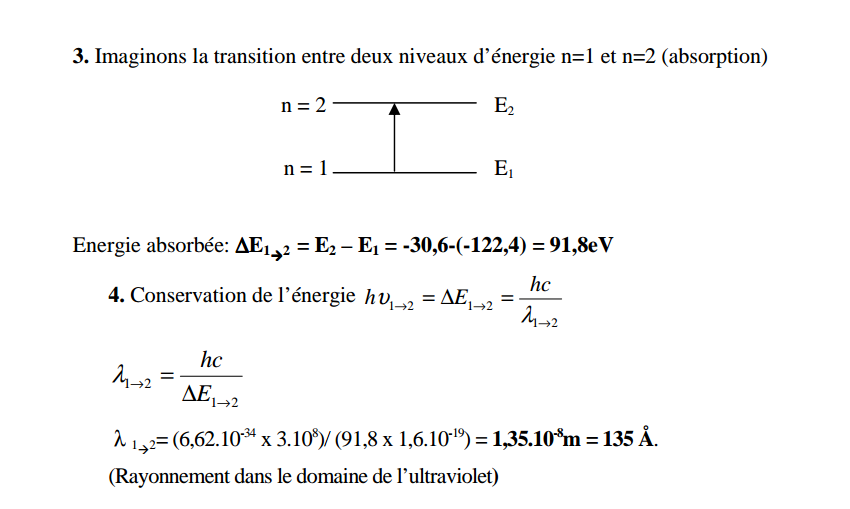
\includegraphics[width=0.55\textwidth]{images/atomistique/atom-004-006.png}
\captionof{figure}{\small Transitions électroniques entre niveaux de Bohr et séries spectrales de l'hydrogène.}
\end{center}
\begin{center}

\includegraphics[width=0.55\textwidth]{images/atomistique/atom-004-007.png}
\captionof{figure}{\small Diagramme des séries de Lyman, Balmer et Paschen dans le spectre de l'hydrogène.}
\end{center}

% ================================================================
\section{Structures électroniques et tableau périodique}
% ================================================================

\subsection*{Exercice 5 - Règles de remplissage des structures électroniques \niveau{\facile}}

\begin{boiteexercice}
Parmi les structures électroniques représentées ci-dessous (voir figure), identifier celles qui ne respectent pas les règles de remplissage et expliquer la règle violée.

\begin{center}
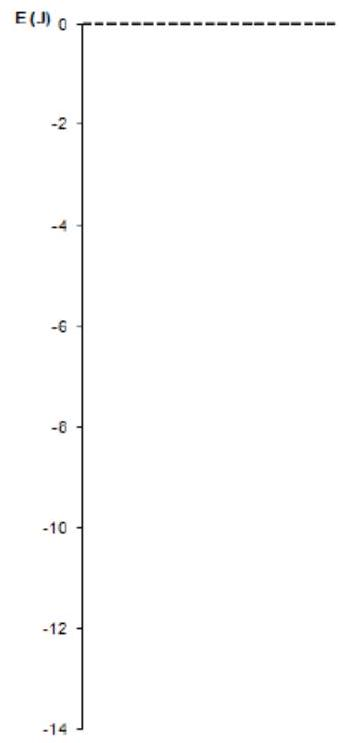
\includegraphics[height=0.55\textheight]{images/atomistique/atom-005-008.png}
\end{center}
\end{boiteexercice}

\begin{boitecorrige}
\begin{itemize}
  \item[(a)] Orbitale $s$ : deux électrons à spins parallèles dans la même case. Violation de la \textbf{règle de Pauli} (deux électrons d'une même case doivent avoir des spins antiparallèles).
  \item[(c)] Orbitale $s$ remplie avant une orbitale de niveau inférieur : violation de la \textbf{règle de Klechkowski} (remplissage dans le mauvais ordre d'énergie).
  \item[(d)] Orbitale $p$ : la première case est vide alors que la deuxième est remplie. Violation de la \textbf{règle de Hund} (il faut distribuer les électrons dans le maximum de cases avant d'en remplir une).
  \item[(e)] Remplissage des sous-couches dans un ordre non conforme à Klechkowski : violation de la \textbf{règle de Klechkowski}.
  \item[(f)] Sous-couche $d$ : des électrons sont appariés avant que toutes les cases soient singly occupied. Violation de la \textbf{règle de Hund}.
\end{itemize}
\end{boitecorrige}

\subsection*{Exercice 6 - Configurations électroniques : N, P et As \niveau{\difficile}}

\begin{boiteexercice}
On considère les éléments $\text{N}_{7}$, $\text{P}_{15}$ et $\text{As}_{33}$.

\begin{enumerate}
  \item Établir leurs configurations électroniques.
  \item Préciser leur position dans le tableau périodique.
  \item Comparer leur électronégativité $\chi$.
  \item Expliquer pourquoi la réaction du chlore avec le phosphore peut conduire à $\text{PCl}_3$ et $\text{PCl}_5$, alors qu'avec l'azote seul $\text{NCl}_3$ se forme. (On note que le chlore est plus électronégatif que l'azote.)
  \item (a) Donner la structure de Lewis de $\text{NH}_3$, $\text{PH}_3$ et $\text{AsH}_3$, et prévoir leur géométrie. (b) Comparer leurs angles de liaison.
  \item Donner la configuration électronique des espèces PN et PN$^+$ et en déduire leurs propriétés magnétiques et le type de liaison.
\end{enumerate}
\end{boiteexercice}

\begin{boitecorrige}
\textbf{1. Configurations électroniques :}
\[
\text{N}_{7} : 1s^{2}\,2s^{2}\,2p^{3} \qquad \text{P}_{15} : 1s^{2}\,2s^{2}\,2p^{6}\,3s^{2}\,3p^{3} \qquad \text{As}_{33} : [\text{Ar}]\,4s^{2}\,3d^{10}\,4p^{3}
\]

\textbf{2. Position dans le tableau :} Ces trois éléments appartiennent à la colonne VA (groupe 15), respectivement aux périodes 2, 3 et 4.

\textbf{3. Électronégativité :} Sur une même colonne, l'électronégativité diminue de haut en bas car le rayon atomique augmente (l'attraction sur les électrons liants est plus faible). Ainsi : $\chi_N > \chi_P > \chi_{As}$.

\textbf{4.} Le phosphore appartient à la troisième période et possède des orbitales $3d$ vides accessibles. Par promotion électronique, il peut porter 5 électrons de valence dans les liaisons, ce qui permet la formation de $\text{PCl}_5$. L'azote, appartenant à la deuxième période, \textbf{ne dispose d'aucune orbitale $d$}. Il ne peut donc pas dépasser la valence 3 (octet strict). La formation de $\text{NCl}_5$ est impossible.

\textbf{5.(a)} Les trois molécules $\text{NH}_3$, $\text{PH}_3$ et $\text{AsH}_3$ ont une géométrie \textbf{pyramidale trigonale} (ou tétraèdre irrégulier) car l'atome central possède un doublet non liant. La structure de Lewis de $\text{NH}_3$ : N avec un doublet libre et trois liaisons N--H.

\textbf{5.(b)} L'angle de liaison $\widehat{\text{HXH}}$ est d'autant plus grand que l'atome central X est électronégatif, car il attire fortement les doublets liants, ce qui accroît la répulsion entre les liaisons. On a donc : $\widehat{\text{HNH}} > \widehat{\text{HPH}} > \widehat{\text{HAsH}}$ (valeurs expérimentales : $107{,}8^\circ $, $93{,}3^\circ $, $91{,}8^\circ $).

\textbf{6.} La molécule PN possède $5 + 5 = 10$ électrons de valence, distribués dans 10 orbitales moléculaires.

Configuration OM de PN (analogie N$_2$) :
\[
\sigma_{2s}^{2}\,\sigma^{*2}_{2s}\,(\pi_{2p_x},\pi_{2p_y})^{4}\,\sigma_{2p_z}^{2}
\]
Tous les électrons sont appariés : PN est \textbf{diamagnétique}. L'indice de liaison $\omega = \frac{(2+4+2)-(2)}{2} = \frac{6}{2} = 3$ : triple liaison (une $\sigma$ et deux $\pi$).

Pour PN$^+$, on retire un électron liant de $\sigma_{2p_z}$ :
\[
\sigma_{2s}^{2}\,\sigma^{*2}_{2s}\,(\pi_{2p_x},\pi_{2p_y})^{4}\,\sigma_{2p_z}^{1}
\]
Un électron célibataire : PN$^+$ est \textbf{paramagnétique}. Indice de liaison $\omega' = 2{,}5$.
\end{boitecorrige}

\begin{center}
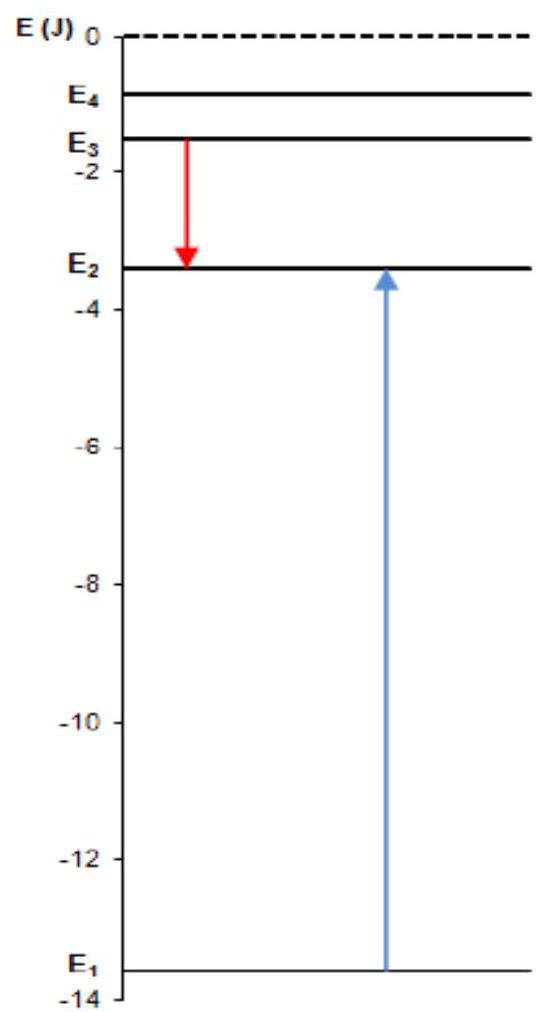
\includegraphics[height=0.55\textheight]{images/atomistique/atom-006-009.png}
\captionof{figure}{\small Diagramme d'énergie des orbitales moléculaires de la molécule PN.}
\end{center}
\begin{center}
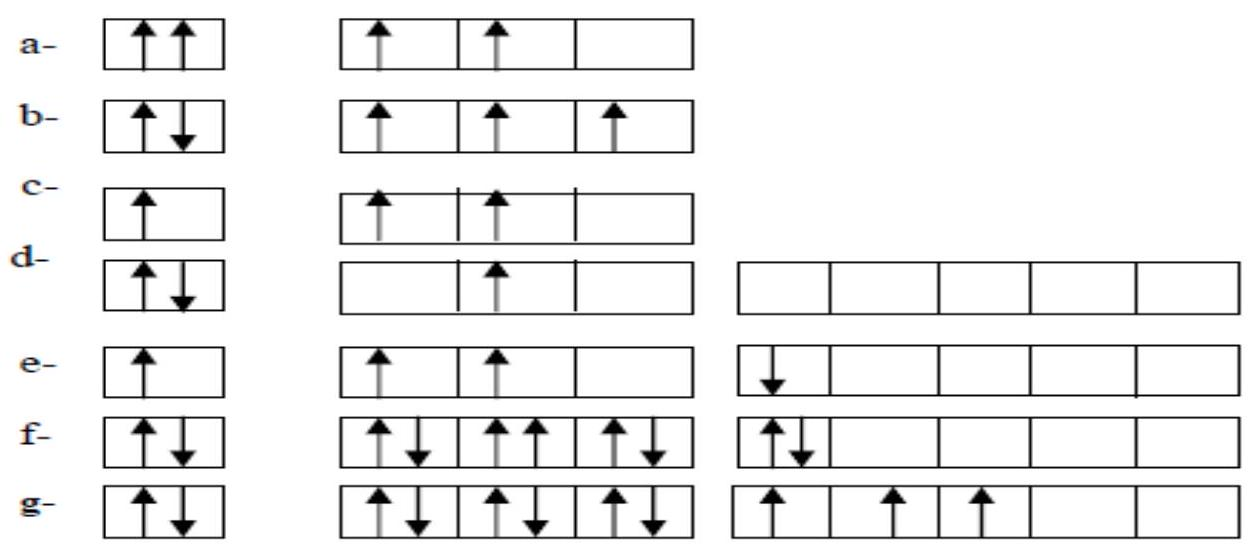
\includegraphics[width=0.55\textwidth]{images/atomistique/atom-006-010.png}
\captionof{figure}{\small Structure de Lewis et géométrie des molécules $\text{NH}_3$, $\text{PH}_3$ et $\text{AsH}_3$.}
\end{center}

\subsection*{Exercice 7 - Identification d'éléments chimiques \niveau{\moyen}}

\begin{boiteexercice}
Donner le numéro atomique et la configuration électronique des éléments suivants :
\begin{enumerate}[label=(\alph*)]
  \item L'halogène de numéro atomique inférieur à 18.
  \item Le gaz rare de même période que le chlore ($Z=17$).
  \item Le troisième halogène.
  \item Le deuxième métal de transition.
  \item Les trois premiers éléments des alcalino-terreux.
\end{enumerate}
\end{boiteexercice}

\begin{boitecorrige}
\begin{enumerate}[label=(\alph*)]
  \item L'halogène de $Z < 18$ : \textbf{Cl}, $Z = 17$ : $[\text{Ne}]\,3s^2\,3p^5$.
  \item Le gaz rare de même période que Cl (période 3) : \textbf{Ar}, $Z = 18$ : $[\text{Ne}]\,3s^2\,3p^6$.
  \item Les halogènes dans l'ordre sont F, Cl, Br... Le troisième est \textbf{Br}, $Z = 35$ : $[\text{Ar}]\,4s^2\,3d^{10}\,4p^5$.
  \item Les métaux de transition commencent en période 4 par Sc ($Z=21$) puis \textbf{Ti} ($Z=22$). Le deuxième métal de transition est donc \textbf{Ti}, $Z = 22$ : $[\text{Ar}]\,4s^2\,3d^2$.
  \item Les alcalino-terreux (groupe 2) : \textbf{Be} ($Z=4$), \textbf{Mg} ($Z=12$), \textbf{Ca} ($Z=20$).
\end{enumerate}
\end{boitecorrige}

\begin{center}
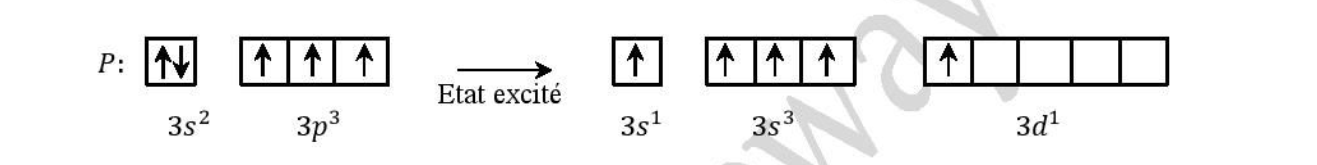
\includegraphics[width=0.55\textwidth]{images/atomistique/atom-007-011.png}
\captionof{figure}{\small Configuration électronique et règle de Klechkowski pour les éléments de transition.}
\end{center}
\begin{center}

\includegraphics[width=0.55\textwidth]{images/atomistique/atom-007-012.png}
\captionof{figure}{\small Tableau périodique : évolution du rayon atomique et de l'électronégativité.}
\end{center}

\subsection*{Exercice 8 - Configurations électroniques des ions X, Y et Z \niveau{\moyen}}

\begin{boiteexercice}
Donner les configurations électroniques des éléments X, Y et Z sachant que :
\begin{enumerate}[label=(\alph*)]
  \item $X^{3+}$ possède la configuration du Néon ($Z_{\text{Ne}}=10$).
  \item Y appartient à la même période que X, et il lui manque deux électrons pour avoir la configuration d'un gaz rare.
  \item $Z^+$ possède la configuration du gaz rare de la même période que Y.
\end{enumerate}
\end{boiteexercice}

\begin{boitecorrige}
\textbf{(a)} Si $X^{3+}$ a la configuration de Ne (10 électrons), alors X possède $10 + 3 = 13$ électrons. C'est l'Aluminium (Al, $Z = 13$) :
\[
_{13}\text{Al} : [\text{Ne}]\,3s^2\,3p^1
\]

\textbf{(b)} X est en période 3 (puisque $Z=13$). Y est dans la même période, et il lui manque 2 électrons pour atteindre la configuration d'Ar ($Z=18$). Donc Y a $18 - 2 = 16$ électrons : c'est le Soufre (S, $Z=16$) :
\[
_{16}\text{S} : [\text{Ne}]\,3s^2\,3p^4
\]

\textbf{(c)} Y est en période 3, le gaz rare de cette période est Ar ($Z=18$). Si $Z^+$ a la configuration d'Ar (18 électrons), alors Z possède $18 + 1 = 19$ électrons : c'est le Potassium (K, $Z=19$) :
\[
_{19}\text{K} : [\text{Ar}]\,4s^1
\]
\end{boitecorrige}

\begin{center}
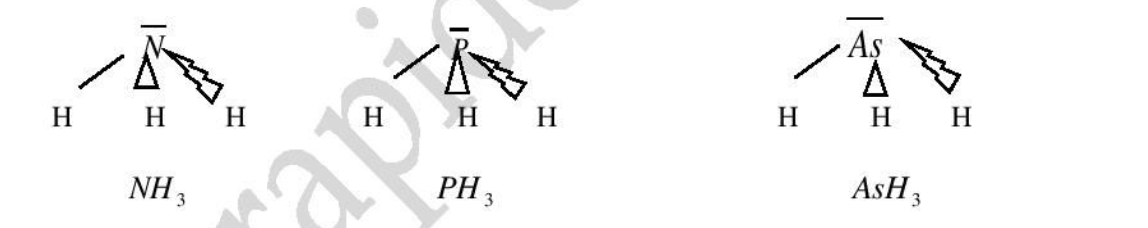
\includegraphics[width=0.55\textwidth]{images/atomistique/atom-008-013.png}
\captionof{figure}{\small Diagramme énergétique des orbitales moléculaires de $\text{O}_2$ : configuration $\sigma$ et $\pi$.}
\end{center}
\begin{center}

\includegraphics[width=0.55\textwidth]{images/atomistique/atom-008-014.png}
\captionof{figure}{\small Structure de Lewis et géométrie des molécules du second exercice.}
\end{center}

% ================================================================
\section{Liaisons chimiques et orbitales moléculaires}
% ================================================================

\subsection*{Exercice 9 - Énergie d'ionisation et affinité électronique \niveau{\moyen}}

\begin{boiteexercice}
L'énergie d'ionisation (EI) est l'énergie nécessaire pour arracher un électron à un atome à l'état gazeux. L'affinité électronique (AE) est l'énergie libérée lors de la capture d'un électron.
\begin{enumerate}
  \item Donner la configuration électronique de Na ($Z=11$), Mg ($Z=12$), Al ($Z=13$) et Si ($Z=14$).
  \item Expliquer pourquoi l'EI de Mg est supérieure à celle de Na, et pourquoi l'EI d'Al est inférieure à celle de Mg.
  \item Comparer les rayons atomiques de Na, Mg, Al et Si. Expliquer la tendance générale.
  \item L'ion $\text{Na}^+$ et l'atome Ne ont-ils la même configuration électronique ? Comparer leurs rayons.
\end{enumerate}
\end{boiteexercice}

\begin{boitecorrige}
\textbf{1. Configurations électroniques :}
\[
\text{Na} : [\text{Ne}]\,3s^1 \qquad \text{Mg} : [\text{Ne}]\,3s^2 \qquad \text{Al} : [\text{Ne}]\,3s^2\,3p^1 \qquad \text{Si} : [\text{Ne}]\,3s^2\,3p^2
\]

\textbf{2.} Mg possède la sous-couche $3s^2$ entièrement remplie, ce qui confère une stabilité particulière (paire d'électrons appariés). Il faut donc plus d'énergie pour ioniser Mg que Na. L'EI de Mg est supérieure à celle de Na.

Cependant, Al a un électron $3p^1$ qui est légèrement plus haut en énergie et plus éloigné du noyau que les électrons $3s^2$ de Mg. Cet électron $3p$ est aussi moins bien blindé. Résultat : l'EI d'Al est \textit{inférieure} à celle de Mg, malgré $Z$ plus grand.

\textbf{3.} Sur une même période, en allant de gauche à droite, le numéro atomique $Z$ augmente, donc l'attraction nucléaire sur les électrons de valence est plus forte. Le rayon atomique \textbf{diminue} : $r_{\text{Na}} > r_{\text{Mg}} > r_{\text{Al}} > r_{\text{Si}}$.

\textbf{4.} $\text{Na}^+$ a perdu un électron : $[\text{Ne}]\,3s^0 \equiv [\text{Ne}]$. Oui, $\text{Na}^+$ et Ne ont la même configuration à 10 électrons. Cependant, Na$^+$ a $Z=11$ contre $Z=10$ pour Ne : l'attraction nucléaire plus forte de Na$^+$ contracte davantage le nuage électronique. Donc $r_{\text{Na}^+} < r_{\text{Ne}}$.
\end{boitecorrige}

\subsection*{Exercice 10 - Orbitales moléculaires de $\text{O}_2$ \niveau{\difficile}}

\begin{boiteexercice}
La molécule $\text{O}_2$ ($Z_O = 8$) est formée de deux atomes d'oxygène.
\begin{enumerate}
  \item Rappeler la configuration électronique de l'atome O.
  \item Écrire la configuration électronique de $\text{O}_2$ dans le cadre de la théorie des orbitales moléculaires (OM). L'ordre des OM pour $\text{O}_2$ est :
  $\sigma_{1s} < \sigma^*_{1s} < \sigma_{2s} < \sigma^*_{2s} < \sigma_{2p_z} < (\pi_{2p_x},\pi_{2p_y}) < (\pi^*_{2p_x},\pi^*_{2p_y}) < \sigma^*_{2p_z}$.
  \item Calculer l'indice de liaison de $\text{O}_2$.
  \item $\text{O}_2$ est-il paramagnétique ou diamagnétique ? Expliquer.
  \item Comparer $\text{O}_2$, $\text{O}_2^+$ et $\text{O}_2^-$ du point de vue de l'indice de liaison et de la longueur de liaison.
\end{enumerate}
\end{boiteexercice}

\begin{boitecorrige}
\textbf{1.} $\text{O}$ ($Z=8$) : $1s^2\,2s^2\,2p^4$.

\textbf{2.} O$_2$ a $2\times8=16$ électrons. Configuration OM :
\[
(\sigma_{1s})^2\,(\sigma^*_{1s})^2\,(\sigma_{2s})^2\,(\sigma^*_{2s})^2\,(\sigma_{2p_z})^2\,(\pi_{2p_x})^2\,(\pi_{2p_y})^2\,(\pi^*_{2p_x})^1\,(\pi^*_{2p_y})^1
\]

\textbf{3.} Électrons liants $N_l = 2+2+2+2+2 = 10$, antiliants $N_{al} = 2+2+1+1 = 6$. Indice de liaison :
\[
\omega = \frac{N_l - N_{al}}{2} = \frac{10-6}{2} = 2
\]
Double liaison (une $\sigma$ et une $\pi$ nette), ce qui correspond bien à la formule de Lewis de O$_2$.

\textbf{4.} Les deux derniers électrons occupent chacun une OM antiliante $\pi^*$ différente, avec des spins parallèles (règle de Hund appliquée aux OM dégénérées). Il y a donc deux électrons célibataires : O$_2$ est \textbf{paramagnétique}. Ceci est confirmé expérimentalement (O$_2$ liquide est attirée par un aimant).

\textbf{5.}
\begin{center}
\begin{tabular}{lccc}
\toprule
Espèce & Électrons & $\omega$ & Liaison\\
\midrule
$\text{O}_2^+$ & 15 & $(10-5)/2 = 2{,}5$ & plus courte\\
$\text{O}_2$ & 16 & $(10-6)/2 = 2$ & référence\\
$\text{O}_2^-$ & 17 & $(10-7)/2 = 1{,}5$ & plus longue\\
\bottomrule
\end{tabular}
\end{center}
Plus l'indice de liaison est élevé, plus la liaison est courte et forte.
\end{boitecorrige}

\subsection*{Exercice 11 - Structure de Lewis et géométrie moléculaire \niveau{\moyen}}

\begin{boiteexercice}
Donner la structure de Lewis et prévoir la géométrie VSEPR (méthode des doublets) des molécules suivantes :
\begin{enumerate}[label=(\alph*)]
  \item $\text{H}_2\text{O}$ (eau)
  \item $\text{CO}_2$ (dioxyde de carbone)
  \item $\text{SO}_2$ (dioxyde de soufre)
  \item $\text{PCl}_5$ (pentachlorure de phosphore)
  \item $\text{SF}_6$ (hexafluorure de soufre)
\end{enumerate}
\end{boiteexercice}

\begin{boitecorrige}
La méthode VSEPR compte les doublets liants et non liants autour de l'atome central, puis minimise les répulsions.

\textbf{(a) H$_2$O :} O central, 2 liaisons O--H (2 doublets liants) et 2 doublets non liants. Formule $AX_2E_2$. Géométrie des atomes : \textbf{coudée}. Angle H--O--H $\approx 104{,}5^\circ$ (inférieur à $109{,}5^\circ$ à cause des doublets libres).

\textbf{(b) CO$_2$ :} C central, 2 doubles liaisons C=O (2 doublets liants effectifs, pas de doublet libre). Formule $AX_2$. Géométrie : \textbf{linéaire}. Angle O=C=O $= 180^\circ$.

\textbf{(c) SO$_2$ :} S central, 1 double liaison S=O, 1 simple liaison S--O et 1 doublet non liant. Formule $AX_2E_1$. Géométrie : \textbf{coudée}. Angle O--S--O $\approx 119^\circ$.

\textbf{(d) PCl$_5$ :} P central, 5 liaisons (pas de doublet libre). Formule $AX_5$. Géométrie : \textbf{bipyramide trigonale}. 3 atomes en position équatoriale ($120^\circ$) et 2 en position axiale ($90^\circ$).

\textbf{(e) SF$_6$ :} S central, 6 liaisons S--F. Formule $AX_6$. Géométrie : \textbf{octaédrique}. Tous les angles F--S--F adjacents sont de $90^\circ$.
\end{boitecorrige}

\subsection*{Exercice 12 - Spectroscopie atomique : séries de l'hydrogène \niveau{\moyen}}

\begin{boiteexercice}
Le spectre de l'atome d'hydrogène est organisé en séries. La série de Balmer correspond aux transitions vers $n_f = 2$, la série de Lyman vers $n_f = 1$, la série de Paschen vers $n_f = 3$.
\begin{enumerate}
  \item Donner la formule générale du nombre d'onde $\tilde{\nu} = 1/\lambda$ pour une transition $n_i \to n_f$ dans l'atome d'hydrogène, en faisant intervenir la constante de Rydberg $R_H = \qty{1.097e7}{m^{-1}}$.
  \item Calculer les longueurs d'onde des trois premières raies de la série de Balmer ($n_i = 3,4,5 \to n_f = 2$).
  \item À quel domaine spectral appartient chaque série (Lyman, Balmer, Paschen) ?
  \item Calculer l'énergie d'ionisation de l'atome d'hydrogène à partir du niveau fondamental.
\end{enumerate}
\end{boiteexercice}

\begin{boitecorrige}
\textbf{1.} La formule de Rydberg-Balmer :
\[
\tilde{\nu} = \frac{1}{\lambda} = R_H\left(\frac{1}{n_f^2} - \frac{1}{n_i^2}\right) \quad (n_i > n_f)
\]

\textbf{2. Série de Balmer} ($n_f = 2$) :
\begin{itemize}[nosep]
  \item $n_i = 3$ (raie $H_\alpha$) : $\tilde{\nu} = 1{,}097\times10^7(1/4 - 1/9) = 1{,}097\times10^7\times5/36 \approx 1{,}524\times10^6\,\text{m}^{-1}$, $\lambda = \qty{656}{nm}$ (rouge).
  \item $n_i = 4$ (raie $H_\beta$) : $\tilde{\nu} = 1{,}097\times10^7(1/4-1/16) = 2{,}057\times10^6\,\text{m}^{-1}$, $\lambda = \qty{486}{nm}$ (vert).
  \item $n_i = 5$ (raie $H_\gamma$) : $\tilde{\nu} = 1{,}097\times10^7(1/4-1/25) = 2{,}304\times10^6\,\text{m}^{-1}$, $\lambda = \qty{434}{nm}$ (violet).
\end{itemize}

\textbf{3.}
\begin{itemize}[nosep]
  \item Lyman ($n_f=1$) : transitions vers le fondamental, $\lambda$ dans l'ultraviolet (UV, 91--122 nm).
  \item Balmer ($n_f=2$) : $\lambda$ dans le visible (400--656 nm).
  \item Paschen ($n_f=3$) : $\lambda$ dans l'infrarouge proche (820 nm--1,87 $\mu$m).
\end{itemize}

\textbf{4. Énergie d'ionisation} depuis $n=1$ : transition $n=1 \to n=\infty$ :
\[
\Delta E = E_\infty - E_1 = 0 - (-13{,}6\,\text{eV}) = \qty{13.6}{eV} = \qty{2.18e-18}{J}
\]
\end{boitecorrige}

\subsection*{Exercice 13 - Radioactivité et décroissance \niveau{\moyen}}

\begin{boiteexercice}
Le carbone 14 ($^{14}_6$C) est un isotope radioactif de période de demi-vie $T_{1/2} = 5730$ ans. Il se désintègre par émission $\beta^-$.
\begin{enumerate}
  \item Écrire l'équation de désintégration du $^{14}_6$C par émission $\beta^-$.
  \item Donner la loi de décroissance radioactive $N(t)$ en fonction du nombre initial $N_0$, de $T_{1/2}$ et du temps $t$.
  \item Quelle fraction de $^{14}_6$C reste après $3\,T_{1/2}$ ?
  \item Un échantillon de bois fossilisé présente une activité de $0{,}15$ Bq/g, alors que le bois vivant a une activité de $0{,}23$ Bq/g. Estimer l'âge de l'échantillon.
\end{enumerate}
\end{boiteexercice}

\begin{boitecorrige}
\textbf{1.} L'émission $\beta^-$ transforme un neutron en proton + électron + antineutrino :
\[
^{14}_6\text{C} \to ^{14}_7\text{N} + e^- + \bar{\nu}_e
\]
Le numéro de masse $A=14$ est conservé ; le numéro atomique passe de 6 à 7.

\textbf{2.} Loi de décroissance :
\[
N(t) = N_0\,2^{-t/T_{1/2}} = N_0\,\e^{-\lambda t} \quad \text{avec}\quad \lambda = \frac{\ln 2}{T_{1/2}}
\]

\textbf{3.} Après $3\,T_{1/2}$ :
\[
\frac{N(3T_{1/2})}{N_0} = 2^{-3} = \frac{1}{8} = 12{,}5\,\%
\]

\textbf{4.} L'activité $A(t) \propto N(t)$, donc $A(t)/A_0 = 2^{-t/T_{1/2}}$ :
\[
\frac{0{,}15}{0{,}23} = 2^{-t/5730} \quad \Rightarrow \quad t = -5730\times\frac{\ln(0{,}15/0{,}23)}{\ln 2} = -5730\times\frac{-0{,}427}{0{,}693} \approx 3531\,\text{ans}
\]
L'échantillon a environ \textbf{3500 ans}.
\end{boitecorrige}


\subsection*{Exercice 14 - Liaison ionique et énergie de réseau \niveau{\moyen}}

\begin{boiteexercice}
On considère la formation du cristal de chlorure de sodium NaCl à partir des atomes isolés Na et Cl.

\begin{enumerate}
  \item Écrire les équations correspondant aux processus suivants et donner leur nom :
    \begin{enumerate}[label=(\alph*)]
      \item Ionisation de Na : $\text{Na}(g) \to \text{Na}^+(g) + e^-$ \quad ($E_I = +\qty{502}{kJ.mol^{-1}}$)
      \item Affinité électronique de Cl : $\text{Cl}(g) + e^- \to \text{Cl}^-(g)$ \quad ($E_{AE} = -\qty{349}{kJ.mol^{-1}}$)
      \item Formation du cristal depuis les ions : $\text{Na}^+(g) + \text{Cl}^-(g) \to \text{NaCl}(s)$ \quad (énergie de réseau $U$)
    \end{enumerate}
  \item En utilisant le cycle de Born-Haber, sachant que l'enthalpie de formation de NaCl(s) depuis les atomes est $\Delta H_f = -\qty{411}{kJ.mol^{-1}}$ et que l'énergie de sublimation de Na est $\Delta H_{sub} = +\qty{108}{kJ.mol^{-1}}$, et la dissociation de Cl$_2$ donne $\Delta H_{diss} = +\qty{121}{kJ.mol^{-1}}$ (par mole de Cl), calculer l'énergie de réseau $U$.
  \item La liaison ionique Na$^+$--Cl$^-$ est-elle favorable sur le plan énergétique ? Justifier.
  \item Comparer l'électronégativité de Na ($\chi = 0{,}93$) et de Cl ($\chi = 3{,}16$). La liaison est-elle purement ionique ?
\end{enumerate}

\textbf{Données :} Toutes les énergies sont données par mole.
\end{boiteexercice}

\begin{boitecorrige}
\textbf{1. Processus et noms :}
\begin{enumerate}[label=(\alph*)]
  \item $\text{Na}(g) \to \text{Na}^+(g) + e^-$ : \textbf{première énergie d'ionisation} de Na.\\ $E_I = +\qty{502}{kJ.mol^{-1}}$ (endothermique).
  \item $\text{Cl}(g) + e^- \to \text{Cl}^-(g)$ : \textbf{affinité électronique} de Cl.\\ $E_{AE} = -\qty{349}{kJ.mol^{-1}}$ (exothermique).
  \item $\text{Na}^+(g) + \text{Cl}^-(g) \to \text{NaCl}(s)$ : \textbf{énergie de réseau} (ou énergie réticulaire) $U$.
\end{enumerate}

\textbf{2. Cycle de Born-Haber.}

Le cycle complet depuis les éléments standard Na(s) et $\frac{1}{2}$Cl$_2$(g) jusqu'à NaCl(s) :
\[
\Delta H_f = \Delta H_{sub}(\text{Na}) + E_I(\text{Na}) + \Delta H_{diss}(\text{Cl}) + E_{AE}(\text{Cl}) + U
\]
En isolant $U$ :
\[
U = \Delta H_f - \Delta H_{sub} - E_I - \Delta H_{diss} - E_{AE}
\]
\[
U = (-411) - (+108) - (+502) - (+121) - (-349)
\]
\[
U = -411 - 108 - 502 - 121 + 349 = \boxed{-\qty{793}{kJ.mol^{-1}}}
\]
L'énergie de réseau est fortement négative (exothermique) : la formation du cristal à partir des ions est très favorable.

\textbf{3.} Le bilan global $E_I + E_{AE} = 502 + (-349) = +\qty{153}{kJ.mol^{-1}}$ est endothermique : la simple réunion des ions gazeux en paires n'est pas favorable. C'est l'organisation cristalline (énergie de réseau $U = -\qty{793}{kJ.mol^{-1}}$) qui rend la formation de NaCl exothermique. La liaison ionique est bien favorable grâce à l'empilement en réseau tridimensionnel.

\textbf{4.} La différence d'électronégativité est $\Delta\chi = 3{,}16 - 0{,}93 = 2{,}23 > 1{,}7$. Par le critère de Pauling, une différence supérieure à $1{,}7$ indique un \textbf{caractère ionique majoritaire}. Cependant, la liaison n'est pas \textit{purement} ionique ; elle possède une part de covalence ($\approx 30\,\%$). On parle de liaisons à \textbf{caractère ionique dominant}.
\end{boitecorrige}

\subsection*{Exercice 15 - Rayons X et niveaux d'énergie des atomes lourds \niveau{\difficile}}

\begin{boiteexercice}
Les rayons X caractéristiques d'un atome sont émis lors de transitions entre couches électroniques profondes. Pour l'atome de cuivre Cu ($Z = 29$) :

\begin{enumerate}
  \item Donner la configuration électronique complète du Cu. (Note : le Cu présente une exception à la règle de Klechkowski ; sa configuration réelle est $[\text{Ar}]\,3d^{10}\,4s^1$. Justifier cette exception.)
  \item Les niveaux d'énergie des couches $K$ ($n=1$), $L$ ($n=2$) et $M$ ($n=3$) pour Cu sont approximativement :
  $E_K = -\qty{8979}{eV}$, $E_L = -\qty{952}{eV}$, $E_M = -\qty{75}{eV}$.
  \begin{enumerate}[label=(\alph*)]
    \item Calculer l'énergie du photon X émis lors de la transition $L \to K$ (raie $K_\alpha$).
    \item Calculer l'énergie du photon X émis lors de la transition $M \to K$ (raie $K_\beta$).
  \end{enumerate}
  \item Calculer les longueurs d'onde correspondantes $\lambda_{K_\alpha}$ et $\lambda_{K_\beta}$ en nm.
  \item À quel domaine du spectre électromagnétique appartiennent ces rayonnements ?
\end{enumerate}

\textbf{Données :} $h = \qty{6.626e-34}{J.s}$, $c = \qty{3.00e8}{m.s^{-1}}$, $\qty{1}{eV} = \qty{1.602e-19}{J}$.
\end{boiteexercice}

\begin{boitecorrige}
\textbf{1. Configuration électronique du Cu ($Z=29$).}

La règle de Klechkowski prédit $[\text{Ar}]\,3d^9\,4s^2$, mais la configuration réelle est :
\[
\text{Cu} : [\text{Ar}]\,3d^{10}\,4s^1
\]
L'exception s'explique par la \textbf{stabilité particulière d'une sous-couche $d$ complète} ($3d^{10}$) : une sous-couche entièrement remplie est énergétiquement plus stable qu'une sous-couche presque remplie ($3d^9$). L'énergie gagnée à compléter la sous-couche $3d$ compense le coût de ne mettre qu'un seul électron en $4s$.

\textbf{2. Énergies des photons X.}

\textbf{(a) Raie $K_\alpha$ (transition $L \to K$) :}
\[
\Delta E_{K_\alpha} = E_K - E_L = (-\qty{8979}{eV}) - (-\qty{952}{eV}) = -\qty{8027}{eV}
\]
Le photon emporte l'énergie $|{\Delta E}| = \qty{8027}{eV}$. En joules :
\[
E_{K_\alpha} = 8027 \times 1{,}602\times10^{-19} = \qty{1.286e-15}{J}
\]

\textbf{(b) Raie $K_\beta$ (transition $M \to K$) :}
\[
\Delta E_{K_\beta} = E_K - E_M = -8979 - (-75) = -\qty{8904}{eV}
\]
\[
E_{K_\beta} = 8904 \times 1{,}602\times10^{-19} = \qty{1.426e-15}{J}
\]

\textbf{3. Longueurs d'onde.}

\[
\lambda_{K_\alpha} = \frac{hc}{E_{K_\alpha}} = \frac{6{,}626\times10^{-34}\times3{,}00\times10^8}{1{,}286\times10^{-15}} = \frac{1{,}988\times10^{-25}}{1{,}286\times10^{-15}} \approx \qty{0.1545}{nm}
\]

\[
\lambda_{K_\beta} = \frac{hc}{E_{K_\beta}} = \frac{1{,}988\times10^{-25}}{1{,}426\times10^{-15}} \approx \qty{0.1394}{nm}
\]

\textbf{4. Domaine spectral.}

Les longueurs d'onde $\lambda_{K_\alpha} \approx \qty{0.154}{nm}$ et $\lambda_{K_\beta} \approx \qty{0.139}{nm}$ sont de l'ordre de \textbf{quelques dixièmes de nanomètre} : elles appartiennent au domaine des \textbf{rayons X} (entre $10^{-2}$ et $10$ nm). Ces longueurs d'onde sont du même ordre de grandeur que les distances interatomiques dans les cristaux, ce qui explique pourquoi les rayons X sont utilisés en diffractométrie pour déterminer les structures cristallographiques.
\end{boitecorrige}


\subsection*{Exercice 16 - Effet photoélectrique et dualité onde-corpuscule \niveau{\moyen}}

\begin{boiteexercice}
L'effet photoélectrique est l'émission d'électrons par un métal illuminé par un rayonnement de fréquence suffisante. Le modèle d'Einstein (1905) postule que la lumière est composée de photons d'énergie $E = h\nu$.

\begin{enumerate}
  \item Pour un métal de travail d'extraction $W_0 = \qty{4.5}{eV}$ (platine), calculer la fréquence seuil $\nu_0$ et la longueur d'onde seuil $\lambda_0$ en dessous de laquelle il n'y a pas d'émission photoélectrique.

  \item On éclaire ce métal avec un rayonnement ultraviolet de longueur d'onde $\lambda = \qty{200}{nm}$. Calculer :
  \begin{enumerate}[label=(\alph*)]
    \item L'énergie du photon incident.
    \item L'énergie cinétique maximale $E_{c,max}$ des photoélectrons émis.
    \item La vitesse maximale $v_{max}$ de ces électrons.
  \end{enumerate}

  \item La dualité onde-corpuscule. De Broglie (1924) propose que toute particule de quantité de mouvement $p$ est associée à une longueur d'onde $\lambda_{dB} = h/p$.
  \begin{enumerate}[label=(\alph*)]
    \item Calculer la longueur d'onde de De Broglie de l'électron émis à la vitesse $v_{max}$.
    \item Calculer la longueur d'onde de De Broglie d'une bille de $m = \qty{1}{g}$ lancée à $v = \qty{1}{m.s^{-1}}$. Commenter.
  \end{enumerate}

  \item Le principe d'Heisenberg : $\Delta x\cdot\Delta p \geq \hbar/2$. Si un électron est localisé dans une boîte de taille $\Delta x = \qty{0.1}{nm}$ (ordre de grandeur atomique), estimer l'incertitude minimale sur sa vitesse.
\end{enumerate}

\textbf{Données :} $h = \qty{6.626e-34}{J.s}$, $\hbar = h/(2\pi)$, $c = \qty{3.00e8}{m.s^{-1}}$, $m_e = \qty{9.109e-31}{kg}$, $\qty{1}{eV} = \qty{1.602e-19}{J}$.
\end{boiteexercice}

\begin{boitecorrige}
\textbf{1. Fréquence et longueur d'onde seuil.}

À la limite ($E_{c,max} = 0$), l'énergie du photon est entièrement utilisée pour extraire l'électron :
\[
h\nu_0 = W_0 = \qty{4.5}{eV} = 4{,}5\times1{,}602\times10^{-19} = \qty{7.209e-19}{J}
\]
\[
\nu_0 = \frac{W_0}{h} = \frac{7{,}209\times10^{-19}}{6{,}626\times10^{-34}} \approx \qty{1.088e15}{Hz}
\]
\[
\lambda_0 = \frac{c}{\nu_0} = \frac{3{,}00\times10^8}{1{,}088\times10^{15}} \approx \qty{275.7}{nm}
\]
Seul le rayonnement UV de longueur d'onde $\lambda < \qty{276}{nm}$ provoque l'effet photoélectrique sur le platine.

\textbf{2. Éclairage par $\lambda = \qty{200}{nm}$ (UV).}

\textbf{(a)} Énergie du photon :
\[
E_{photon} = \frac{hc}{\lambda} = \frac{6{,}626\times10^{-34}\times3{,}00\times10^8}{200\times10^{-9}} = \frac{1{,}988\times10^{-25}}{2\times10^{-7}} = \qty{9.94e-19}{J}
\]
En eV : $E_{photon} = 9{,}94\times10^{-19}/(1{,}602\times10^{-19}) \approx \qty{6.21}{eV}$.

\textbf{(b)} Énergie cinétique maximale (loi d'Einstein) :
\[
E_{c,max} = h\nu - W_0 = 6{,}21 - 4{,}5 = \qty{1.71}{eV} = \qty{2.74e-19}{J}
\]

\textbf{(c)} Vitesse maximale :
\[
\frac{1}{2}m_e v_{max}^2 = E_{c,max} \quad \Rightarrow \quad v_{max} = \sqrt{\frac{2E_{c,max}}{m_e}} = \sqrt{\frac{2\times2{,}74\times10^{-19}}{9{,}109\times10^{-31}}}
\]
\[
v_{max} = \sqrt{6{,}015\times10^{11}} \approx \qty{7.76e5}{m.s^{-1}} \approx \qty{776}{km.s^{-1}}
\]

\textbf{3. Dualité onde-corpuscule.}

\textbf{(a)} Longueur d'onde de De Broglie de l'électron ($v_{max} \approx \qty{7.76e5}{m.s^{-1}}$) :
\[
p_e = m_e v_{max} = 9{,}109\times10^{-31}\times7{,}76\times10^5 = \qty{7.069e-25}{kg.m.s^{-1}}
\]
\[
\lambda_{dB}(e^-) = \frac{h}{p_e} = \frac{6{,}626\times10^{-34}}{7{,}069\times10^{-25}} \approx \qty{9.37e-10}{m} \approx \qty{0.937}{nm}
\]
Cette longueur d'onde est de l'ordre de grandeur des distances atomiques : les électrons peuvent diffracter sur les réseaux cristallins.

\textbf{(b)} Longueur d'onde de De Broglie de la bille ($m = \qty{1e-3}{kg}$, $v = \qty{1}{m.s^{-1}}$) :
\[
p = mv = 10^{-3}\times1 = \qty{1e-3}{kg.m.s^{-1}}
\]
\[
\lambda_{dB}(\text{bille}) = \frac{h}{p} = \frac{6{,}626\times10^{-34}}{10^{-3}} = \qty{6.626e-31}{m}
\]
Cette longueur d'onde est $\approx 10^{21}$ fois plus petite que la taille d'un noyau atomique ($\approx 10^{-15}$ m). Les effets quantiques sont totalement négligeables à l'échelle macroscopique : c'est pourquoi nous n'observons pas de comportement ondulatoire pour les objets de la vie courante.

\textbf{4. Principe d'incertitude d'Heisenberg.}

\[
\Delta p \geq \frac{\hbar}{2\Delta x} = \frac{h}{4\pi\Delta x} = \frac{6{,}626\times10^{-34}}{4\pi\times10^{-10}} = \frac{6{,}626\times10^{-34}}{1{,}257\times10^{-9}} \approx \qty{5.27e-25}{kg.m.s^{-1}}
\]
\[
\Delta v = \frac{\Delta p}{m_e} = \frac{5{,}27\times10^{-25}}{9{,}109\times10^{-31}} \approx \qty{5.79e5}{m.s^{-1}}
\]
L'incertitude sur la vitesse est de l'ordre de $\qty{580}{km.s^{-1}}$, soit presque la vitesse de l'électron lui-même. Cela montre que la notion de trajectoire bien définie n'a pas de sens à l'échelle atomique.
\end{boitecorrige}

\ifdefined\inMainDoc\else\end{document}\fi


% ================================================================
%  UE 2 : ALGÈBRE LINÉAIRE
% ================================================================
\newpage
\thispagestyle{empty}
\begin{tikzpicture}[remember picture, overlay]
  \fill[gray!12] ([xshift=1.5cm, yshift=3cm]current page.south west)
    rectangle ([xshift=-1.5cm, yshift=-3cm]current page.north east);
  \draw[line width=3pt] ([xshift=1.5cm,yshift=-3cm]current page.north west)
    -- ([xshift=-1.5cm,yshift=-3cm]current page.north east);
  \draw[line width=3pt] ([xshift=1.5cm,yshift=3cm]current page.south west)
    -- ([xshift=-1.5cm,yshift=3cm]current page.south east);
  \node[align=center] at (current page.center) {%
    {\fontsize{36}{44}\bfseries\selectfont ALGÈBRE LINÉAIRE}\\[1.2cm]
    {\large\itshape Espaces vectoriels - Matrices - Déterminants}\\[0.4cm]
    {\large\itshape Valeurs propres et diagonalisation}\\[1.8cm]
    {\normalsize Licence 1 - UE 2}
  };
  \node[anchor=south west] at ([xshift=2cm,yshift=2cm]current page.south west)
    {\large\bfseries UE 2};
\end{tikzpicture}
\newpage

\addcontentsline{toc}{section}{ALGÈBRE LINÉAIRE}
\ifdefined\inMainDoc\else
\documentclass[12pt,a4paper]{article}
% ================================================================
%  PRÉAMBULE COMMUN - ANNALES CORRIGÉES
%  Université de Kara - FaST - Licence Fondamentale MPC
%  Design optimisé impression noir et blanc
% ================================================================

% -- ENCODAGE & LANGUE --
\usepackage[utf8]{inputenc}
\usepackage[T1]{fontenc}
\usepackage[french]{babel}
\usepackage{lmodern}
\usepackage{microtype}

% -- MISE EN PAGE --
\usepackage[a4paper, top=2.8cm, bottom=2.5cm, left=2.5cm, right=2.5cm, headheight=14pt]{geometry}
\usepackage{setspace}
\setstretch{1.2}
\usepackage{parskip}
\setlength{\parindent}{1.2em}
\setlength{\parskip}{4pt}

% -- MATHS --
\usepackage{amsmath, amssymb, mathtools, amsthm}
\usepackage{mathrsfs}
\usepackage{dsfont}
\usepackage{bm}
\usepackage{cancel}
\usepackage{textcomp}
% Définition de \oiint (intégrale de surface fermée) sans package supplémentaire
\newcommand{\oiint}{\mathop{\iint\!\!\!\!\!\!\!\bigcirc}\limits}

% -- PHYSIQUE & CHIMIE --
\usepackage{physics}
\usepackage{siunitx}
% Lorsque physics est chargé, siunitx omet \qty. On le restaure ici :
\AtBeginDocument{\RenewCommandCopy\qty\SI}
\sisetup{locale = FR, detect-all, output-decimal-marker={,}}
% Commande de substitution pour les unités posant problème avec pdflatex
% (ohm, degreeCelsius, micro, angstrom, percent utilisent des caractères non-ASCII)
\newcommand{\qtyohm}[1]{\ensuremath{\num{#1}\,\Omega}}
\newcommand{\qtydegc}[1]{\ensuremath{\num{#1}\,{}^\circ\text{C}}}
\newcommand{\qtyangstrom}[1]{\ensuremath{\num{#1}\,\text{\AA}}}
\newcommand{\qtypercent}[1]{\ensuremath{\num{#1}\,\%}}
\newcommand{\qtyum}[1]{\ensuremath{\num{#1}\,\mu\text{m}}}
\usepackage[version=4]{mhchem}

% -- GRAPHISMES --
\usepackage{graphicx}
\usepackage{float}
\usepackage{caption}
\usepackage{subcaption}
\usepackage{wrapfig}
\usepackage{tikz}
\usetikzlibrary{calc, arrows.meta, patterns, shapes.geometric}
\usepackage{pgfplots}
\pgfplotsset{compat=1.18}

% -- TABLEAUX --
\usepackage{booktabs}
\usepackage{array}
\usepackage{tabularx}
\usepackage{multirow}

% -- LISTES --
\usepackage{enumitem}
\setlist[enumerate]{topsep=3pt, itemsep=2pt, parsep=0pt}
\setlist[itemize]{topsep=3pt, itemsep=2pt, parsep=0pt, label={.}}

% -- BOÎTES (noir et blanc) --
\usepackage{mdframed}
\usepackage{tcolorbox}
\tcbuselibrary{skins, breakable, theorems}

% Boîte EXERCICE : encadré avec filet épais, fond blanc
\newmdenv[
  linewidth=1.2pt,
  linecolor=black,
  roundcorner=3pt,
  skipabove=10pt,
  skipbelow=6pt,
  innertopmargin=8pt,
  innerbottommargin=8pt,
  innerleftmargin=10pt,
  innerrightmargin=10pt,
  backgroundcolor=white,
  frametitle={\bfseries\small Exercice},
  frametitlealignment=\raggedright,
  frametitleaboveskip=4pt,
  frametitlebelowskip=4pt,
]{boiteexercice}

% Boîte CORRIGÉ : fond gris très clair + filet fin
\newmdenv[
  linewidth=0.6pt,
  linecolor=black,
  leftline=true,
  rightline=false,
  topline=false,
  bottomline=false,
  linecolor=black,
  innerleftmargin=12pt,
  innerrightmargin=8pt,
  innertopmargin=6pt,
  innerbottommargin=6pt,
  backgroundcolor=gray!8,
  skipabove=4pt,
  skipbelow=8pt,
]{boitecorrige}

% Boîte RÉSUMÉ DE COURS : double encadré
\newmdenv[
  linewidth=0.8pt,
  linecolor=black,
  roundcorner=2pt,
  backgroundcolor=gray!12,
  innertopmargin=10pt,
  innerbottommargin=10pt,
  innerleftmargin=12pt,
  innerrightmargin=12pt,
  skipabove=12pt,
  skipbelow=8pt,
]{boiteresume}

% Boîte ATTENTION/REMARQUE : barre gauche épaisse
\newmdenv[
  leftline=true,
  rightline=false,
  topline=false,
  bottomline=false,
  linewidth=3pt,
  linecolor=black,
  backgroundcolor=gray!5,
  innerleftmargin=12pt,
  innerrightmargin=8pt,
  innertopmargin=5pt,
  innerbottommargin=5pt,
  skipabove=6pt,
  skipbelow=6pt,
]{boiteremarque}

% -- DIFFICULTÉ DES EXERCICES --
\newcommand{\facile}{$\star$}
\newcommand{\moyen}{$\star\!\star$}
\newcommand{\difficile}{$\star\!\star\!\star$}
\newcommand{\niveau}[1]{\hfill\textbf{#1}\hspace{2pt}}

% -- EN-TÊTES ET PIEDS DE PAGE --
\usepackage{fancyhdr}
\pagestyle{fancy}
\fancyhf{}
\renewcommand{\headrulewidth}{0.5pt}
\renewcommand{\footrulewidth}{0.3pt}

% -- HYPERLIENS --
\usepackage[hidelinks]{hyperref}
\hypersetup{
    colorlinks=false,
    pdftitle={Annale Corrigée - Licence MPC - Université de Kara}
}

% -- TITRES --
\usepackage{titlesec}
\titleformat{\section}{\Large\bfseries}{\thesection.}{0.8em}{}[\vspace{2pt}\hrule\vspace{4pt}]
\titleformat{\subsection}{\large\bfseries}{\thesubsection.}{0.7em}{}
\titleformat{\subsubsection}{\normalsize\bfseries}{\thesubsubsection.}{0.6em}{}

% -- THÉORÈMES --
\theoremstyle{definition}
\newtheorem{defn}{Définition}[section]
\newtheorem{prop}{Propriété}[section]
\newtheorem{thm}{Théorème}[section]
\newtheorem{corol}{Corollaire}[section]
\newtheorem{exemple}{Exemple}[section]

% -- COMMANDES MATHÉMATIQUES UTILES --
\newcommand{\vect}[1]{\overrightarrow{#1}}
\newcommand{\R}{\mathbb{R}}
\newcommand{\N}{\mathbb{N}}
\newcommand{\Z}{\mathbb{Z}}
\newcommand{\C}{\mathbb{C}}
\renewcommand{\d}{\mathrm{d}}
\newcommand{\deriv}[2]{\dfrac{\d #1}{\d #2}}
\newcommand{\dpart}[2]{\dfrac{\partial #1}{\partial #2}}
\newcommand{\rot}{\overrightarrow{\mathrm{rot}}\,}
\renewcommand{\div}{\mathrm{div}\,}
\renewcommand{\grad}{\overrightarrow{\mathrm{grad}}\,}
\newcommand{\e}{\mathrm{e}}
\newcommand{\ii}{\mathrm{i}}
\renewcommand{\Tr}{\mathrm{Tr}}

% Numérotation des équations par section
\numberwithin{equation}{section}

% -- RÉSULTATS ENCADRÉS --
\newcommand{\res}[1]{\[\boxed{#1}\]}

% -- REMARQUE INLINE --
\newcommand{\rmq}[1]{\begin{boiteremarque}\textbf{Remarque.} #1\end{boiteremarque}}

% -- MISE EN VALEUR DU RÉSULTAT FINAL --
\newcommand{\reponse}[1]{%
  \begin{center}
    \fbox{\begin{minipage}{0.92\textwidth}\centering #1\end{minipage}}
  \end{center}%
}


\lhead{\small\textit{Algèbre Linéaire - Licence 1}}
\rhead{\small\textit{FaST, Université de Kara}}
\cfoot{\thepage}

\begin{document}
\fi

\begin{center}
  {\LARGE\bfseries ALGÈBRE LINÉAIRE}\\[0.3cm]
  {\normalsize Licence 1 - Mathématiques, Physique et Chimie}\\[0.1cm]
  \rule{0.7\textwidth}{0.8pt}
\end{center}

\section*{Résumé du cours}

\begin{boiteresume}

\textbf{1. Espaces vectoriels.} Un ensemble $E$ muni d'une addition et d'une multiplication scalaire est un espace vectoriel sur $\mathbb{R}$ s'il vérifie les 8 axiomes (associativité, distributivité, élément neutre $\vec{0}$, opposé, etc.). Une famille $(\vec{e}_1,\ldots,\vec{e}_n)$ est une \textit{base} de $E$ si elle est libre (aucun vecteur combinaison des autres) et génératrice ($E = \text{vect}(\vec{e}_1,\ldots,\vec{e}_n)$). La dimension de $E$ est le nombre de vecteurs dans toute base.

\textbf{2. Applications linéaires.} Une application $f : E \to F$ est linéaire si $f(\alpha\vec{u}+\beta\vec{v}) = \alpha f(\vec{u})+\beta f(\vec{v})$ pour tous $\alpha,\beta\in\mathbb{R}$ et $\vec{u},\vec{v}\in E$. Le noyau $\ker f = \{\vec{x}\in E \mid f(\vec{x})=\vec{0}\}$ et l'image $\text{Im}\,f = \{f(\vec{x}) \mid \vec{x}\in E\}$. Théorème du rang : $\dim(\ker f) + \dim(\text{Im}\,f) = \dim E$.

\textbf{3. Matrices.} Une matrice $A\in\mathcal{M}_{m,n}(\mathbb{R})$ représente une application linéaire dans des bases. Le produit $AB$ est défini si le nombre de colonnes de $A$ égale le nombre de lignes de $B$ : $(AB)_{ij} = \sum_k a_{ik}b_{kj}$. Une matrice $A$ est inversible si et seulement si $\det A \neq 0$.

\textbf{4. Déterminants.} Pour $A\in\mathcal{M}_n(\mathbb{R})$, le déterminant vérifie : $\det(AB)=\det A\cdot\det B$, $\det(A^T)=\det A$. Calcul par développement selon une ligne ou cofacteurs.

\textbf{5. Valeurs propres et vecteurs propres.} $\lambda$ est valeur propre de $A$ si $\exists\vec{x}\neq\vec{0}$ tel que $A\vec{x}=\lambda\vec{x}$. Les valeurs propres sont les racines du polynôme caractéristique $P_A(\lambda) = \det(A-\lambda I)$. La matrice est diagonalisable si et seulement si elle possède $n$ vecteurs propres linéairement indépendants.

\textbf{6. Systèmes linéaires.} Le système $A\vec{x}=\vec{b}$ est résolu par la méthode de Gauss (échelonnement). Il admet une solution unique si $\det A\neq 0$, une infinité de solutions si $A$ est singulière et $\vec{b}\in\text{Im}\,A$, ou aucune solution sinon.

\end{boiteresume}

\newpage
\section{Espaces vectoriels et bases}

\subsection*{Exercice 1 - Sous-espaces vectoriels \niveau{\facile}}

\begin{boiteexercice}
Dans $\mathbb{R}^3$, déterminer parmi les ensembles suivants lesquels sont des sous-espaces vectoriels :
\begin{enumerate}[label=(\alph*)]
  \item $F = \{(x,y,z)\in\mathbb{R}^3 \mid x + 2y - z = 0\}$
  \item $G = \{(x,y,z)\in\mathbb{R}^3 \mid x^2 + y^2 = 0\}$
  \item $H = \{(x,y,z)\in\mathbb{R}^3 \mid x + y + z = 1\}$
  \item $K = \{(x,y,z)\in\mathbb{R}^3 \mid x = y = 0\}$
\end{enumerate}
\end{boiteexercice}

\begin{boitecorrige}
Pour être un sous-espace vectoriel, un ensemble doit : (i) contenir $\vec{0}$, (ii) être stable par addition, (iii) être stable par multiplication scalaire.

\textbf{(a) $F$ est un sous-espace vectoriel.}
$\vec{0}$: $0+2(0)-0=0$. Stabilité: si $\vec{u},\vec{v}\in F$, alors $(x_1+2y_1-z_1)+(x_2+2y_2-z_2)=0+0=0$, donc $\vec{u}+\vec{v}\in F$. Scalaire: $\alpha(x_1+2y_1-z_1)=\alpha\cdot0=0$. C'est le plan de vecteur normal $(1,2,-1)$.

\textbf{(b) $G$ est un sous-espace vectoriel.}
$x^2+y^2=0$ avec $x,y\in\mathbb{R}$ implique $x=y=0$. Donc $G=\{(0,0,z)\mid z\in\mathbb{R}\}$, qui est l'axe $(Oz)$, bien un sous-espace.

\textbf{(c) $H$ n'est pas un sous-espace vectoriel.}
$\vec{0}\notin H$ car $0+0+0=0\neq1$.

\textbf{(d) $K$ est un sous-espace vectoriel.}
$K=\{(0,0,z)\mid z\in\mathbb{R}\}$ est l'axe $(Oz)$. Mêmes vérifications immédiates.
\end{boitecorrige}

\subsection*{Exercice 2 - Base et dimension \niveau{\facile}}

\begin{boiteexercice}
On considère les vecteurs $\vec{u}_1=(1,1,0)$, $\vec{u}_2=(0,1,1)$, $\vec{u}_3=(1,0,-1)$ de $\mathbb{R}^3$.
\begin{enumerate}
  \item Ces vecteurs forment-ils une base de $\mathbb{R}^3$ ?
  \item Exprimer $\vec{v}=(2,3,1)$ dans cette base.
\end{enumerate}
\end{boiteexercice}

\begin{boitecorrige}
\textbf{1.} On calcule le déterminant :
\[
\det\begin{pmatrix}1&0&1\\1&1&0\\0&1&-1\end{pmatrix}
= 1\cdot(1\cdot(-1)-0\cdot1) - 0 + 1\cdot(1\cdot1-1\cdot0)
= (-1) + (1) = -2 + 2
\]
Développons correctement : $1(1\cdot(-1)-0\cdot1) - 0(1\cdot(-1)-0\cdot0) + 1(1\cdot1-1\cdot0) = -1+0+1=0$.

Hmm, recalculons avec la matrice dont les colonnes sont $\vec{u}_1,\vec{u}_2,\vec{u}_3$ :
\[
\det\begin{pmatrix}1&0&1\\1&1&0\\0&1&-1\end{pmatrix}
= 1\begin{vmatrix}1&0\\1&-1\end{vmatrix} - 0 + 1\begin{vmatrix}1&1\\0&1\end{vmatrix}
= 1(-1-0) + 1(1-0) = -1+1 = 0
\]
Le déterminant est nul : les vecteurs ne forment \textbf{pas} une base de $\mathbb{R}^3$. Ils sont liés.

On vérifie : $\vec{u}_3 = \vec{u}_1 - \vec{u}_2$ (car $(1,0,-1)=(1,1,0)-(0,1,1)$). Les trois vecteurs sont donc coplanaires.

\textbf{2.} Puisque $(\vec{u}_1,\vec{u}_2,\vec{u}_3)$ n'est pas une base, on ne peut pas toujours exprimer $\vec{v}$ de façon unique. On cherche $\alpha,\beta,\gamma$ tels que $\alpha\vec{u}_1+\beta\vec{u}_2+\gamma\vec{u}_3=\vec{v}$ :
\[
\begin{cases}\alpha+\gamma=2\\\alpha+\beta=3\\\beta-\gamma=1\end{cases}
\]
De la 2e et 3e : $\beta=\gamma+1$, donc $\alpha = 3-\beta = 2-\gamma$. Substitution dans la 1re : $(2-\gamma)+\gamma=2$. La solution a un paramètre libre : $\gamma=t$, $\beta=t+1$, $\alpha=2-t$ pour tout $t\in\mathbb{R}$. Par exemple pour $t=0$ : $\vec{v} = 2\vec{u}_1 + \vec{u}_2 + 0\vec{u}_3$.
\end{boitecorrige}

\section{Matrices et déterminants}

\subsection*{Exercice 3 - Opérations matricielles \niveau{\facile}}

\begin{boiteexercice}
Soient $A = \begin{pmatrix}1&2\\3&4\end{pmatrix}$ et $B = \begin{pmatrix}-1&0\\2&1\end{pmatrix}$.
\begin{enumerate}
  \item Calculer $AB$, $BA$, $A+2B$ et $A^T$.
  \item Calculer $\det A$, $\det B$ et $\det(AB)$.
  \item La matrice $A$ est-elle inversible ? Si oui, calculer $A^{-1}$.
\end{enumerate}
\end{boiteexercice}

\begin{boitecorrige}
\textbf{1.}
\[
AB = \begin{pmatrix}1(-1)+2(2) & 1(0)+2(1)\\ 3(-1)+4(2) & 3(0)+4(1)\end{pmatrix}
= \begin{pmatrix}3&2\\5&4\end{pmatrix}
\]
\[
BA = \begin{pmatrix}(-1)(1)+0(3) & (-1)(2)+0(4)\\ 2(1)+1(3) & 2(2)+1(4)\end{pmatrix}
= \begin{pmatrix}-1&-2\\5&8\end{pmatrix}
\]
$AB \neq BA$ : le produit matriciel n'est pas commutatif en général.
\[
A+2B = \begin{pmatrix}1-2&2+0\\3+4&4+2\end{pmatrix} = \begin{pmatrix}-1&2\\7&6\end{pmatrix}, \quad A^T = \begin{pmatrix}1&3\\2&4\end{pmatrix}
\]

\textbf{2.} $\det A = 1\times4 - 2\times3 = 4-6 = -2$. $\det B = (-1)(1)-(0)(2) = -1$. $\det(AB) = \det A\cdot\det B = (-2)(-1) = 2$. Vérification : $\det\begin{pmatrix}3&2\\5&4\end{pmatrix}=12-10=2$.

\textbf{3.} $\det A = -2 \neq 0$, donc $A$ est inversible :
\[
A^{-1} = \frac{1}{-2}\begin{pmatrix}4&-2\\-3&1\end{pmatrix} = \begin{pmatrix}-2&1\\3/2&-1/2\end{pmatrix}
\]
Vérification : $AA^{-1} = \begin{pmatrix}1(- 2)+2(3/2) & 1(1)+2(-1/2)\\ 3(-2)+4(3/2) & 3(1)+4(-1/2)\end{pmatrix} = \begin{pmatrix}-2+3 & 1-1\\ -6+6 & 3-2\end{pmatrix} = I$.
\end{boitecorrige}

\subsection*{Exercice 4 - Résolution de systèmes linéaires \niveau{\moyen}}

\begin{boiteexercice}
Résoudre les systèmes suivants par la méthode de Gauss :
\begin{enumerate}[label=(\alph*)]
  \item $\begin{cases}2x + y - z = 3\\ x - y + 2z = -1\\ 3x + 2y + z = 4\end{cases}$

  \item $\begin{cases}x + 2y + z = 2\\ 2x + 4y + 2z = 4\\ x + y - z = 1\end{cases}$
\end{enumerate}
\end{boiteexercice}

\begin{boitecorrige}
\textbf{(a)} Matrice augmentée :
\[
\begin{pmatrix}2&1&-1&\mid&3\\1&-1&2&\mid&-1\\3&2&1&\mid&4\end{pmatrix}
\xrightarrow{L_1\leftrightarrow L_2}
\begin{pmatrix}1&-1&2&\mid&-1\\2&1&-1&\mid&3\\3&2&1&\mid&4\end{pmatrix}
\]
\[
\xrightarrow{L_2-2L_1,\;L_3-3L_1}
\begin{pmatrix}1&-1&2&\mid&-1\\0&3&-5&\mid&5\\0&5&-5&\mid&7\end{pmatrix}
\xrightarrow{L_3-\frac{5}{3}L_2}
\begin{pmatrix}1&-1&2&\mid&-1\\0&3&-5&\mid&5\\0&0&\frac{10}{3}&\mid&\frac{-4}{3}\end{pmatrix}
\]
De la 3e ligne : $z = \frac{-4/3}{10/3} = -\frac{2}{5}$. De la 2e : $3y = 5+5z = 5-2 = 3$, donc $y=1$. De la 1re : $x = -1+y-2z = -1+1+\frac{4}{5} = \frac{4}{5}$.
\[
\boxed{x = \frac{4}{5},\quad y = 1,\quad z = -\frac{2}{5}}
\]

\textbf{(b)} La 2e équation est $2\times$ la 1re (dépendante). Après élimination :
\[
\begin{pmatrix}1&2&1&\mid&2\\0&0&0&\mid&0\\0&-1&-2&\mid&-1\end{pmatrix}
\xrightarrow{L_2\leftrightarrow L_3}
\begin{pmatrix}1&2&1&\mid&2\\0&-1&-2&\mid&-1\\0&0&0&\mid&0\end{pmatrix}
\]
De la 2e : $y = 1-2z$. De la 1re : $x = 2-2y-z = 2-2(1-2z)-z = 3z$. Solution à un paramètre libre $z=t\in\mathbb{R}$ :
\[
\boxed{(x,y,z) = (3t,\;1-2t,\;t), \quad t\in\mathbb{R}}
\]
\end{boitecorrige}

\section{Valeurs propres et diagonalisation}

\subsection*{Exercice 5 - Valeurs propres \niveau{\moyen}}

\begin{boiteexercice}
Soit la matrice $A = \begin{pmatrix}3&1\\1&3\end{pmatrix}$.
\begin{enumerate}
  \item Calculer le polynôme caractéristique et les valeurs propres de $A$.
  \item Déterminer les vecteurs propres associés à chaque valeur propre.
  \item La matrice est-elle diagonalisable ? Si oui, écrire la décomposition $A = PDP^{-1}$.
\end{enumerate}
\end{boiteexercice}

\begin{boitecorrige}
\textbf{1.} $P_A(\lambda) = \det(A-\lambda I) = \det\begin{pmatrix}3-\lambda&1\\1&3-\lambda\end{pmatrix} = (3-\lambda)^2-1 = \lambda^2-6\lambda+8 = (\lambda-2)(\lambda-4)$.

Valeurs propres : $\lambda_1 = 2$ et $\lambda_2 = 4$.

\textbf{2.}
Pour $\lambda_1 = 2$ : $(A-2I)\vec{x}=\vec{0}$ donne $\begin{pmatrix}1&1\\1&1\end{pmatrix}\vec{x}=\vec{0}$, soit $x+y=0$. Vecteur propre : $\vec{v}_1 = \begin{pmatrix}1\\-1\end{pmatrix}$.

Pour $\lambda_2 = 4$ : $(A-4I)\vec{x}=\vec{0}$ donne $\begin{pmatrix}-1&1\\1&-1\end{pmatrix}\vec{x}=\vec{0}$, soit $-x+y=0$. Vecteur propre : $\vec{v}_2 = \begin{pmatrix}1\\1\end{pmatrix}$.

\textbf{3.} $A$ est symétrique réelle, donc diagonalisable (théorème spectral). Les deux vecteurs propres sont linéairement indépendants.
\[
P = \begin{pmatrix}1&1\\-1&1\end{pmatrix}, \quad D = \begin{pmatrix}2&0\\0&4\end{pmatrix}, \quad P^{-1} = \frac{1}{2}\begin{pmatrix}1&-1\\1&1\end{pmatrix}
\]
Vérification : $AP = PD$.
\end{boitecorrige}

\subsection*{Exercice 6 - Matrice $3\times3$ et diagonalisation \niveau{\moyen}}

\begin{boiteexercice}
Soit $A = \begin{pmatrix}2&1&0\\1&2&0\\0&0&3\end{pmatrix}$.
\begin{enumerate}
  \item Calculer les valeurs propres et les espaces propres.
  \item La matrice est-elle diagonalisable ?
  \item Calculer $A^n$ pour $n\in\mathbb{N}$.
\end{enumerate}
\end{boiteexercice}

\begin{boitecorrige}
\textbf{1.} $P_A(\lambda) = \det(A-\lambda I)$. En développant selon la 3e colonne :
\begin{align*}
P_A(\lambda) &= (3-\lambda)\det\begin{pmatrix}2-\lambda&1\\1&2-\lambda\end{pmatrix}\\
&= (3-\lambda)\bigl[(2-\lambda)^2-1\bigr]\\
&= (3-\lambda)(\lambda^2-4\lambda+3)\\
&= (3-\lambda)(3-\lambda)(1-\lambda) = (3-\lambda)^2(1-\lambda)
\end{align*}
Valeurs propres : $\lambda_1=1$ (simple) et $\lambda_2=3$ (double).

Pour $\lambda_1=1$ : $(A-I)\vec{x}=\vec{0}$ donne la matrice :
\[\begin{pmatrix}1&1&0\\1&1&0\\0&0&2\end{pmatrix}\]
soit $x+y=0$ et $z=0$.
\[
E_1 = \text{vect}\begin{pmatrix}1\\-1\\0\end{pmatrix}, \quad \dim E_1=1.
\]

Pour $\lambda_2=3$ : $(A-3I)\vec{x}=\vec{0}$ donne $\begin{pmatrix}-1&1&0\\1&-1&0\\0&0&0\end{pmatrix}$, soit $-x+y=0$.
\[
E_3 = \text{vect}\left\{\begin{pmatrix}1\\1\\0\end{pmatrix},\begin{pmatrix}0\\0\\1\end{pmatrix}\right\}, \quad \dim E_3=2.
\]

\textbf{2.} $\dim E_1+\dim E_3 = 1+2=3=\dim\mathbb{R}^3$. La matrice est \textbf{diagonalisable}.

\textbf{3.} Avec $P = \begin{pmatrix}1&1&0\\-1&1&0\\0&0&1\end{pmatrix}$, on a $A = PDP^{-1}$ avec $D=\text{diag}(1,3,3)$. Donc $A^n = PD^nP^{-1}$ avec $D^n=\text{diag}(1,3^n,3^n)$. Après calcul :
\[
A^n = \frac{1}{2}\begin{pmatrix}1+3^n&3^n-1&0\\3^n-1&1+3^n&0\\0&0&2\cdot3^n\end{pmatrix}
\]
\end{boitecorrige}

\subsection*{Exercice 7 - Application linéaire \niveau{\difficile}}

\begin{boiteexercice}
Soit $f : \mathbb{R}^3 \to \mathbb{R}^3$ l'application définie par $f(x,y,z) = (x+y, y+z, x+z)$.
\begin{enumerate}
  \item Vérifier que $f$ est linéaire.
  \item Déterminer $\ker f$ et $\text{Im}\,f$.
  \item Écrire la matrice de $f$ dans la base canonique.
  \item $f$ est-elle un isomorphisme ?
\end{enumerate}
\end{boiteexercice}

\begin{boitecorrige}
\textbf{1.} Soient $\vec{u}=(x_1,y_1,z_1)$, $\vec{v}=(x_2,y_2,z_2)$ et $\alpha,\beta\in\mathbb{R}$ :
\[
f(\alpha\vec{u}+\beta\vec{v}) = (\alpha x_1+\beta x_2+\alpha y_1+\beta y_2,\;\ldots)
= \alpha f(\vec{u})+\beta f(\vec{v})
\]
Les composantes sont des combinaisons linéaires des coordonnées, donc $f$ est bien linéaire.

\textbf{2.} $\ker f$ : $f(x,y,z)=\vec{0}$ donne
$\begin{cases}x+y=0\\y+z=0\\x+z=0\end{cases}$. De la 1re et 3e : $y=-x$, $z=-x$. Substitution dans la 2e : $-x+(-x)=-2x=0$, donc $x=0$. Ainsi $\ker f=\{\vec{0}\}$.

$\text{Im}\,f$ : par le théorème du rang, $\dim(\text{Im}\,f)=3-\dim(\ker f)=3-0=3$. Donc $\text{Im}\,f=\mathbb{R}^3$.

\textbf{3.} La matrice dans la base canonique est obtenue en appliquant $f$ aux vecteurs de base :
\[
[f] = \begin{pmatrix}1&1&0\\0&1&1\\1&0&1\end{pmatrix}
\]

\textbf{4.} $\ker f=\{\vec{0}\}$, donc $f$ est injective. Comme $\dim\mathbb{R}^3<\infty$ et $f$ est injective de $\mathbb{R}^3$ dans $\mathbb{R}^3$, elle est surjective, donc c'est un \textbf{isomorphisme}. On peut vérifier : $\det[f]=1(1-0)-1(0-1)+0=1+1=2\neq0$.
\end{boitecorrige}

\subsection*{Exercice 8 - Rang d'une matrice \niveau{\moyen}}

\begin{boiteexercice}
Calculer le rang des matrices suivantes :
\begin{enumerate}[label=(\alph*)]
  \item $A = \begin{pmatrix}1&2&3\\2&4&6\\1&1&2\end{pmatrix}$
  \item $B = \begin{pmatrix}1&0&2\\0&1&-1\\2&-1&5\end{pmatrix}$
  \item $C = \begin{pmatrix}1&2&0&1\\2&4&1&3\\0&0&1&1\end{pmatrix}$
\end{enumerate}
\end{boiteexercice}

\begin{boitecorrige}
\textbf{(a)} $L_2 \leftarrow L_2 - 2L_1$, $L_3 \leftarrow L_3 - L_1$ :
\[
\begin{pmatrix}1&2&3\\0&0&0\\0&-1&-1\end{pmatrix}
\xrightarrow{L_2\leftrightarrow L_3}
\begin{pmatrix}1&2&3\\0&-1&-1\\0&0&0\end{pmatrix}
\]
Deux lignes non nulles : $\text{rg}(A) = 2$.

\textbf{(b)} $L_3 \leftarrow L_3 - 2L_1$ puis $L_3 \leftarrow L_3 + L_2$ :
\[
\begin{pmatrix}1&0&2\\0&1&-1\\0&-1&1\end{pmatrix}
\to
\begin{pmatrix}1&0&2\\0&1&-1\\0&0&0\end{pmatrix}
\]
$\text{rg}(B) = 2$.

\textbf{(c)} On travaille sur la matrice $C$ (3 lignes, 4 colonnes). $L_2 \leftarrow L_2 - 2L_1$ :
\[
\begin{pmatrix}1&2&0&1\\0&0&1&1\\0&0&1&1\end{pmatrix}
\xrightarrow{L_3 - L_2}
\begin{pmatrix}1&2&0&1\\0&0&1&1\\0&0&0&0\end{pmatrix}
\]
$\text{rg}(C) = 2$.
\end{boitecorrige}

\subsection*{Exercice 9 - Inverse par la méthode de Gauss-Jordan \niveau{\moyen}}

\begin{boiteexercice}
Calculer l'inverse de la matrice $A = \begin{pmatrix}1&1&0\\0&1&1\\1&0&1\end{pmatrix}$ par la méthode de Gauss-Jordan.
\end{boiteexercice}

\begin{boitecorrige}
On augmente la matrice avec l'identité et on réduit $A$ à $I$ par opérations élémentaires :
\[
\left(\begin{array}{ccc|ccc}1&1&0&1&0&0\\0&1&1&0&1&0\\1&0&1&0&0&1\end{array}\right)
\xrightarrow{L_3-L_1}
\left(\begin{array}{ccc|ccc}1&1&0&1&0&0\\0&1&1&0&1&0\\0&-1&1&-1&0&1\end{array}\right)
\]
\[
\xrightarrow{L_3+L_2}
\left(\begin{array}{ccc|ccc}1&1&0&1&0&0\\0&1&1&0&1&0\\0&0&2&-1&1&1\end{array}\right)
\xrightarrow{L_3/2}
\left(\begin{array}{ccc|ccc}1&1&0&1&0&0\\0&1&1&0&1&0\\0&0&1&-1/2&1/2&1/2\end{array}\right)
\]
\[
\xrightarrow{L_2-L_3}
\left(\begin{array}{ccc|ccc}1&1&0&1&0&0\\0&1&0&1/2&1/2&-1/2\\0&0&1&-1/2&1/2&1/2\end{array}\right)
\xrightarrow{L_1-L_2}
\left(\begin{array}{ccc|ccc}1&0&0&1/2&-1/2&1/2\\0&1&0&1/2&1/2&-1/2\\0&0&1&-1/2&1/2&1/2\end{array}\right)
\]
\[
A^{-1} = \frac{1}{2}\begin{pmatrix}1&-1&1\\1&1&-1\\-1&1&1\end{pmatrix}
\]
Vérification : $\det A = 1(1-0) - 1(0-1) + 0 = 2 \neq 0$.
\end{boitecorrige}

\section{Systèmes linéaires avancés}

\subsection*{Exercice 10 - Règle de Cramer \niveau{\moyen}}

\begin{boiteexercice}
Résoudre le système suivant par la règle de Cramer :
\[
\begin{cases}2x + y - z = 5\\x - y + z = 0\\x + 2y + z = 3\end{cases}
\]
\end{boiteexercice}

\begin{boitecorrige}
La matrice du système est $A = \begin{pmatrix}2&1&-1\\1&-1&1\\1&2&1\end{pmatrix}$.

$\det A = 2(-1-2) - 1(1-1) + (-1)(2+1) = 2(-3) - 0 - 3 = -9$.

Matrices dérivées (on remplace chaque colonne par le second membre $\vec{b} = (5,0,3)^T$) :
\[
D_x = \det\begin{pmatrix}5&1&-1\\0&-1&1\\3&2&1\end{pmatrix} = 5(-1-2)-1(0-3)+(-1)(0+3) = -15+3-3=-15
\]
\[
D_y = \det\begin{pmatrix}2&5&-1\\1&0&1\\1&3&1\end{pmatrix} = 2(0-3)-5(1-1)+(-1)(3-0) = -6-0-3=-9
\]
\[
D_z = \det\begin{pmatrix}2&1&5\\1&-1&0\\1&2&3\end{pmatrix} = 2(-3-0)-1(3-0)+5(2+1) = -6-3+15=6
\]
\[
\boxed{x = \frac{D_x}{\det A} = \frac{-15}{-9} = \frac{5}{3}, \quad y = \frac{D_y}{\det A} = \frac{-9}{-9} = 1, \quad z = \frac{D_z}{\det A} = \frac{6}{-9} = -\frac{2}{3}}
\]
Vérification : $2(5/3)+1-(-2/3) = 10/3+1+2/3 = 12/3+1=5$.
\end{boitecorrige}

\subsection*{Exercice 11 - Déterminant d'une matrice $4\times4$ \niveau{\difficile}}

\begin{boiteexercice}
Calculer le déterminant de la matrice
\[
A = \begin{pmatrix}1&0&2&-1\\3&0&0&5\\2&1&4&-3\\1&0&5&0\end{pmatrix}
\]
par développement selon la colonne qui contient le plus de zéros.
\end{boiteexercice}

\begin{boitecorrige}
On développe selon la colonne 2 (trois zéros) :
\[
\det A = 0\cdot C_{12} + 0\cdot C_{22} + 1\cdot C_{32} + 0\cdot C_{42}
\]
Il ne reste que le cofacteur $C_{32} = (-1)^{3+2}M_{32} = -M_{32}$, où $M_{32}$ est le mineur obtenu en supprimant la ligne 3 et la colonne 2 :
\[
M_{32} = \det\begin{pmatrix}1&2&-1\\3&0&5\\1&5&0\end{pmatrix}
\]
On développe selon la 2e colonne (ou ligne 2) :
\[
= 1(0-25) - 2(0-5) + (-1)(15-0) = -25+10-15 = -30
\]
\[
\det A = 1\times(-(-30)) = 1\times30 = 30
\]

\textbf{Vérification partielle :} Le déterminant d'une matrice triangulaire supérieure serait le produit des termes diagonaux. Ce n'est pas le cas ici, mais on peut vérifier avec le développement selon la ligne 1 comme contrôle.
\end{boitecorrige}

\subsection*{Exercice 12 - Valeurs propres complexes et réduction \niveau{\difficile}}

\begin{boiteexercice}
Soit $A = \begin{pmatrix}0&-1&0\\1&0&0\\0&0&2\end{pmatrix}$.
\begin{enumerate}
  \item Calculer le polynôme caractéristique de $A$.
  \item Déterminer les valeurs propres (dans $\mathbb{C}$) et les sous-espaces propres.
  \item La matrice est-elle diagonalisable sur $\mathbb{R}$ ? Sur $\mathbb{C}$ ?
\end{enumerate}
\end{boiteexercice}

\begin{boitecorrige}
\textbf{1.} En développant selon la 3e colonne (terme $2-\lambda$ en bas à droite) :
\[
P_A(\lambda) = \det(A-\lambda I) = (2-\lambda)\det\begin{pmatrix}-\lambda&-1\\1&-\lambda\end{pmatrix}
= (2-\lambda)(\lambda^2+1)
\]

\textbf{2.} Valeurs propres : $\lambda_1 = 2$ (réelle) et $\lambda_{2,3} = \pm i$ (complexes conjuguées).

Pour $\lambda_1 = 2$ : $(A-2I)\vec{x}=\vec{0}$ : $\begin{pmatrix}-2&-1&0\\1&-2&0\\0&0&0\end{pmatrix}$, soit $-2x-y=0$ et $x-2y=0$. Ces deux équations donnent $x=y=0$, $z$ libre. $E_2 = \text{vect}\begin{pmatrix}0\\0\\1\end{pmatrix}$.

Pour $\lambda_2 = i$ (sur $\mathbb{C}$) : $(A-iI)\vec{x}=\vec{0}$ donne $-ix-y=0$, soit $y=-ix$. Sous-espace propre : $E_i = \text{vect}\begin{pmatrix}1\\-i\\0\end{pmatrix}$.

De même, $E_{-i} = \text{vect}\begin{pmatrix}1\\i\\0\end{pmatrix}$.

\textbf{3.} Les valeurs propres $\pm i$ ne sont pas réelles : $A$ \textbf{n'est pas diagonalisable sur $\mathbb{R}$}. En revanche, elle possède 3 valeurs propres complexes distinctes, donc elle est \textbf{diagonalisable sur $\mathbb{C}$}, avec $D = \text{diag}(2, i, -i)$.
\end{boitecorrige}

\subsection*{Exercice 13 - Espace vectoriel de polynômes \niveau{\moyen}}

\begin{boiteexercice}
Soit $E = \mathbb{R}_2[X]$ l'espace des polynômes de degré au plus 2, et $f : E \to \mathbb{R}^3$ définie par $f(P) = (P(0), P(1), P(2))$.
\begin{enumerate}
  \item Vérifier que $f$ est linéaire.
  \item Calculer $\ker f$ et $\text{Im}\, f$.
  \item En déduire si $f$ est un isomorphisme.
\end{enumerate}
\end{boiteexercice}

\begin{boitecorrige}
\textbf{1.} Pour $P, Q \in E$ et $\alpha, \beta \in \mathbb{R}$ :
\[
f(\alpha P + \beta Q) = ((\alpha P+\beta Q)(0), (\alpha P+\beta Q)(1), (\alpha P+\beta Q)(2))
\]
\[
= (\alpha P(0)+\beta Q(0), \alpha P(1)+\beta Q(1), \alpha P(2)+\beta Q(2)) = \alpha f(P) + \beta f(Q)
\]
Donc $f$ est linéaire.

\textbf{2.} $\ker f = \{P\in E : P(0)=P(1)=P(2)=0\}$. Un polynôme de degré $\leq 2$ ayant 3 racines distinctes est le polynôme nul. Donc $\ker f = \{0\}$.

Par le théorème du rang : $\dim(\text{Im}\,f) = \dim E - \dim(\ker f) = 3 - 0 = 3$. Donc $\text{Im}\,f = \mathbb{R}^3$ (surjective).

\textbf{3.} $f$ est injective ($\ker f = \{0\}$) et surjective. C'est donc un \textbf{isomorphisme}.

Cela signifie que tout triplet $(a, b, c) \in \mathbb{R}^3$ est l'image d'un unique polynôme de degré $\leq 2$ : c'est l'interpolation de Lagrange en $x=0,1,2$.
\end{boitecorrige}

\subsection*{Exercice 14 - Diagonalisation et puissance de matrice \niveau{\difficile}}

\begin{boiteexercice}
Soit $A = \begin{pmatrix}4&-2\\1&1\end{pmatrix}$.
\begin{enumerate}
  \item Calculer les valeurs propres et les vecteurs propres de $A$.
  \item Diagonaliser $A$ et exprimer $A^n$ pour tout $n\in\mathbb{N}$.
  \item Calculer $A^{10}$.
\end{enumerate}
\end{boiteexercice}

\begin{boitecorrige}
\textbf{1.} $P_A(\lambda) = (4-\lambda)(1-\lambda)+2 = \lambda^2-5\lambda+6 = (\lambda-2)(\lambda-3)$.

Valeurs propres : $\lambda_1 = 2$, $\lambda_2 = 3$.

Pour $\lambda_1 = 2$ : $(A-2I)\vec{x}=\vec{0}$ : $2x-2y=0$, soit $\vec{v}_1 = \begin{pmatrix}1\\1\end{pmatrix}$.

Pour $\lambda_2 = 3$ : $(A-3I)\vec{x}=\vec{0}$ : $x-2y=0$, soit $\vec{v}_2 = \begin{pmatrix}2\\1\end{pmatrix}$.

\textbf{2.} $P = \begin{pmatrix}1&2\\1&1\end{pmatrix}$, $D = \begin{pmatrix}2&0\\0&3\end{pmatrix}$, $P^{-1} = \frac{1}{\det P}\begin{pmatrix}1&-2\\-1&1\end{pmatrix} = \begin{pmatrix}-1&2\\1&-1\end{pmatrix}$.

$A^n = PD^nP^{-1} = \begin{pmatrix}1&2\\1&1\end{pmatrix}\begin{pmatrix}2^n&0\\0&3^n\end{pmatrix}\begin{pmatrix}-1&2\\1&-1\end{pmatrix}$

\[
= \begin{pmatrix}2^n&2\cdot3^n\\2^n&3^n\end{pmatrix}\begin{pmatrix}-1&2\\1&-1\end{pmatrix}
= \begin{pmatrix}-2^n+2\cdot3^n & 2^{n+1}-2\cdot3^n \\ -2^n+3^n & 2^{n+1}-3^n\end{pmatrix}
\]

Simplifions : $A^n = \begin{pmatrix}2\cdot3^n-2^n & 2^{n+1}-2\cdot3^n\\3^n-2^n & 2^{n+1}-3^n\end{pmatrix}$.

\textbf{3.} Pour $n=10$ : $2^{10} = 1024$, $3^{10} = 59049$ :
\[
A^{10} = \begin{pmatrix}2\times59049-1024 & 2048-2\times59049\\59049-1024 & 2048-59049\end{pmatrix}
= \begin{pmatrix}117074 & -116050\\58025 & -57001\end{pmatrix}
\]
\end{boitecorrige}


% ================================================================
\subsection*{Exercice 15 - Diagonalisation d'une matrice symétrique \niveau{\moyen}}
% ================================================================
\begin{boiteexercice}
Soit la matrice $A = \begin{pmatrix}5 & 2 \\ 2 & 5\end{pmatrix}$.

\begin{enumerate}
  \item Calculer le polynôme caractéristique de $A$ et en déduire ses valeurs propres.
  \item Déterminer les vecteurs propres associés à chaque valeur propre.
  \item Former la matrice de passage $P$ et la matrice diagonale $D = P^{-1}AP$.
  \item Vérifier que $A = PDP^{-1}$.
\end{enumerate}
\end{boiteexercice}

\begin{boitecorrige}
\textbf{1. Polynôme caractéristique :}
\[
\chi_A(\lambda) = \det(A - \lambda I) = \begin{vmatrix}5-\lambda & 2 \\ 2 & 5-\lambda\end{vmatrix}
= (5-\lambda)^2 - 4 = \lambda^2 - 10\lambda + 21 = (\lambda-3)(\lambda-7)
\]
Les valeurs propres sont $\lambda_1 = 3$ et $\lambda_2 = 7$.

\textbf{2. Vecteurs propres :}

\textit{Pour $\lambda_1 = 3$ :} $(A-3I)\vec{x} = \vec{0}$ :
\[
\begin{pmatrix}2 & 2 \\ 2 & 2\end{pmatrix}\begin{pmatrix}x\\y\end{pmatrix} = \vec{0} \;\Rightarrow\; x+y=0 \;\Rightarrow\; \vec{v}_1 = \begin{pmatrix}1\\-1\end{pmatrix}
\]

\textit{Pour $\lambda_2 = 7$ :} $(A-7I)\vec{x} = \vec{0}$ :
\[
\begin{pmatrix}-2 & 2 \\ 2 & -2\end{pmatrix}\begin{pmatrix}x\\y\end{pmatrix} = \vec{0} \;\Rightarrow\; -x+y=0 \;\Rightarrow\; \vec{v}_2 = \begin{pmatrix}1\\1\end{pmatrix}
\]

\textbf{3. Matrice de passage et diagonalisation :}
\[
P = \begin{pmatrix}1 & 1 \\ -1 & 1\end{pmatrix}, \qquad \det P = 1\cdot1-(-1)\cdot1 = 2
\]
\[
P^{-1} = \frac{1}{2}\begin{pmatrix}1 & -1 \\ 1 & 1\end{pmatrix}
\]
\[
D = P^{-1}AP = \begin{pmatrix}3 & 0 \\ 0 & 7\end{pmatrix}
\]

\textbf{4. Vérification :}
\[
PDP^{-1} = \begin{pmatrix}1&1\\-1&1\end{pmatrix}\begin{pmatrix}3&0\\0&7\end{pmatrix}\frac{1}{2}\begin{pmatrix}1&-1\\1&1\end{pmatrix}
= \frac{1}{2}\begin{pmatrix}3+7 & -3+7\\-3+7 & 3+7\end{pmatrix} = \begin{pmatrix}5&2\\2&5\end{pmatrix} = A \;
\]

\textbf{Remarque :} $A$ est symétrique réelle, donc ses vecteurs propres sont bien orthogonaux : $\vec{v}_1\cdot\vec{v}_2 = 1\cdot1+(-1)\cdot1 = 0$.
\end{boitecorrige}

% ================================================================
\subsection*{Exercice 16 - Forme de Jordan (matrice non diagonalisable) \niveau{\difficile}}
% ================================================================
\begin{boiteexercice}
Soit la matrice $A = \begin{pmatrix}2 & 1 \\ 0 & 2\end{pmatrix}$.

\begin{enumerate}
  \item Calculer le polynôme caractéristique. Quelle est la valeur propre (sa multiplicité algébrique) ?
  \item Trouver le sous-espace propre associé. Quelle est la multiplicité géométrique ?
  \item La matrice est-elle diagonalisable ? Justifier.
  \item Déterminer un vecteur propre généralisé $\vec{w}$ tel que $(A-\lambda I)\vec{w} = \vec{v}$ où $\vec{v}$ est le vecteur propre.
  \item Écrire la forme de Jordan $J$ de $A$ et la matrice de passage $P$ telle que $A = PJP^{-1}$.
\end{enumerate}
\end{boiteexercice}

\begin{boitecorrige}
\textbf{1. Polynôme caractéristique :}
\[
\chi_A(\lambda) = (2-\lambda)^2
\]
Valeur propre unique : $\lambda = 2$ de multiplicité algébrique $m_a = 2$.

\textbf{2. Sous-espace propre :}
\[
A - 2I = \begin{pmatrix}0&1\\0&0\end{pmatrix}
\]
$(A-2I)\vec{x}=\vec{0}$ donne $y=0$, donc $\vec{v}_1 = \begin{pmatrix}1\\0\end{pmatrix}$.
Multiplicité géométrique : $m_g = 1$ (un seul vecteur propre indépendant).

\textbf{3.} Puisque $m_g = 1 < m_a = 2$, la matrice \textbf{n'est pas diagonalisable}.

\textbf{4. Vecteur propre généralisé :}

On cherche $\vec{w}$ tel que $(A-2I)\vec{w} = \vec{v}_1$ :
\[
\begin{pmatrix}0&1\\0&0\end{pmatrix}\begin{pmatrix}w_1\\w_2\end{pmatrix} = \begin{pmatrix}1\\0\end{pmatrix} \;\Rightarrow\; w_2 = 1, \quad w_1 \text{ libre}
\]
On choisit $w_1 = 0$, soit $\vec{w} = \begin{pmatrix}0\\1\end{pmatrix}$.

\textbf{5. Forme de Jordan :}

La base de Jordan est $\mathcal{B} = (\vec{v}_1, \vec{w})$, d'où :
\[
P = \begin{pmatrix}1 & 0 \\ 0 & 1\end{pmatrix} = I, \qquad J = \begin{pmatrix}2 & 1 \\ 0 & 2\end{pmatrix} = A
\]
Dans ce cas, $A$ est \emph{déjà} sous forme de Jordan. On a bien $J = P^{-1}AP$ avec $P=I$.

\textbf{Propriété utile :} $A^n = \begin{pmatrix}2^n & n\cdot2^{n-1}\\0&2^n\end{pmatrix}$. En effet, $(J)^n = \begin{pmatrix}\lambda^n & n\lambda^{n-1}\\0&\lambda^n\end{pmatrix}$ pour un bloc de Jordan $2\times2$.
\end{boitecorrige}

% ================================================================
\subsection*{Exercice 17 - Calcul de $A^n$ par diagonalisation \niveau{\moyen}}
% ================================================================
\begin{boiteexercice}
Soit $A = \begin{pmatrix}2&1\\1&2\end{pmatrix}$.

\begin{enumerate}
  \item Calculer les valeurs propres $\lambda_1$ et $\lambda_2$ de $A$.
  \item Trouver les vecteurs propres associés.
  \item Former la matrice de passage $P$ et calculer $P^{-1}$.
  \item Exprimer $A^n = PD^nP^{-1}$ et simplifier.
  \item Application : calculer $A^5$.
\end{enumerate}
\end{boiteexercice}

\begin{boitecorrige}
\textbf{1. Valeurs propres :}
\[
\chi_A(\lambda) = (2-\lambda)^2 - 1 = \lambda^2 - 4\lambda + 3 = (\lambda-1)(\lambda-3)
\]
$\lambda_1 = 1$, $\lambda_2 = 3$.

\textbf{2. Vecteurs propres :}

\textit{Pour $\lambda_1 = 1$ :} $(A-I)\vec{x}=\vec{0}$ : $x+y=0$, donc $\vec{v}_1 = \begin{pmatrix}1\\-1\end{pmatrix}$.

\textit{Pour $\lambda_2 = 3$ :} $(A-3I)\vec{x}=\vec{0}$ : $-x+y=0$, donc $\vec{v}_2 = \begin{pmatrix}1\\1\end{pmatrix}$.

\textbf{3. Matrice de passage :}
\[
P = \begin{pmatrix}1&1\\-1&1\end{pmatrix}, \quad \det P = 2, \quad P^{-1} = \frac{1}{2}\begin{pmatrix}1&-1\\1&1\end{pmatrix}
\]

\textbf{4.} $D^n = \begin{pmatrix}1^n&0\\0&3^n\end{pmatrix} = \begin{pmatrix}1&0\\0&3^n\end{pmatrix}$, donc :
\[
A^n = PD^nP^{-1} = \begin{pmatrix}1&1\\-1&1\end{pmatrix}\begin{pmatrix}1&0\\0&3^n\end{pmatrix}\frac{1}{2}\begin{pmatrix}1&-1\\1&1\end{pmatrix}
\]
\[
= \frac{1}{2}\begin{pmatrix}1&3^n\\-1&3^n\end{pmatrix}\begin{pmatrix}1&-1\\1&1\end{pmatrix}
= \frac{1}{2}\begin{pmatrix}1+3^n & -1+3^n \\ -1+3^n & 1+3^n\end{pmatrix}
\]

\textbf{5.} Pour $n=5$ : $3^5 = 243$ :
\[
A^5 = \frac{1}{2}\begin{pmatrix}244 & 242 \\ 242 & 244\end{pmatrix} = \begin{pmatrix}122 & 121 \\ 121 & 122\end{pmatrix}
\]
\end{boitecorrige}

% ================================================================
\subsection*{Exercice 18 - Système linéaire compatible indéterminé \niveau{\moyen}}
% ================================================================
\newpage
\begin{boiteexercice}
Résoudre par la méthode de Gauss-Jordan le système suivant à 4 inconnues :
\[
\left\{\begin{aligned}
x_1 + 2x_2 - x_3 + x_4 &= 2 \\
2x_1 + 4x_2 + x_3 - x_4 &= 5 \\
x_1 + 2x_2 + 2x_3 - 2x_4 &= 3
\end{aligned}\right.
\]

\begin{enumerate}
  \item Écrire la matrice augmentée et effectuer les opérations élémentaires sur les lignes.
  \item Identifier le rang du système et les inconnues libres (paramètres).
  \item Exprimer les inconnues liées en fonction des paramètres.
  \item Écrire la solution générale sous forme vectorielle.
\end{enumerate}
\end{boiteexercice}

\begin{boitecorrige}
\textbf{1. Matrice augmentée et réduction :}
\[
\left(\begin{array}{cccc|c}1&2&-1&1&2\\2&4&1&-1&5\\1&2&2&-2&3\end{array}\right)
\]
$L_2 \leftarrow L_2 - 2L_1$ ; $L_3 \leftarrow L_3 - L_1$ :
\[
\left(\begin{array}{cccc|c}1&2&-1&1&2\\0&0&3&-3&1\\0&0&3&-3&1\end{array}\right)
\]
$L_3 \leftarrow L_3 - L_2$ :
\[
\left(\begin{array}{cccc|c}1&2&-1&1&2\\0&0&3&-3&1\\0&0&0&0&0\end{array}\right)
\]
$L_2 \leftarrow L_2/3$ ; $L_1 \leftarrow L_1 + L_2$ :
\[
\left(\begin{array}{cccc|c}1&2&0&0&7/3\\0&0&1&-1&1/3\\0&0&0&0&0\end{array}\right)
\]

\textbf{2.} Le rang est $r=2$. Les colonnes pivots sont 1 et 3. Les inconnues libres (paramètres) sont $x_2 = s$ et $x_4 = t$ ($s,t\in\mathbb{R}$).

\textbf{3.} Des équations réduites :
\begin{align*}
x_1 + 2s &= 7/3 &\Rightarrow& \quad x_1 = 7/3 - 2s \\
x_3 - t &= 1/3  &\Rightarrow& \quad x_3 = 1/3 + t
\end{align*}

\textbf{4. Solution générale sous forme vectorielle :}
\[
\begin{pmatrix}x_1\\x_2\\x_3\\x_4\end{pmatrix}
= \begin{pmatrix}7/3\\0\\1/3\\0\end{pmatrix}
+ s\begin{pmatrix}-2\\1\\0\\0\end{pmatrix}
+ t\begin{pmatrix}0\\0\\1\\1\end{pmatrix}, \quad s,t\in\mathbb{R}
\]

L'espace solution est un \textbf{sous-espace affine} de dimension 2 (plan affine dans $\mathbb{R}^4$). La solution particulière est $\vec{x}_0 = (7/3, 0, 1/3, 0)^T$ et la solution homogène est engendrée par les vecteurs $(-2,1,0,0)^T$ et $(0,0,1,1)^T$.
\end{boitecorrige}

\ifdefined\inMainDoc\else\end{document}\fi


% ================================================================
%  UE 3 : ANALYSE VECTORIELLE
% ================================================================
\newpage
\thispagestyle{empty}
\begin{tikzpicture}[remember picture, overlay]
  \fill[gray!12] ([xshift=1.5cm, yshift=3cm]current page.south west)
    rectangle ([xshift=-1.5cm, yshift=-3cm]current page.north east);
  \draw[line width=3pt] ([xshift=1.5cm,yshift=-3cm]current page.north west)
    -- ([xshift=-1.5cm,yshift=-3cm]current page.north east);
  \draw[line width=3pt] ([xshift=1.5cm,yshift=3cm]current page.south west)
    -- ([xshift=-1.5cm,yshift=3cm]current page.south east);
  \node[align=center] at (current page.center) {%
    {\fontsize{34}{42}\bfseries\selectfont ANALYSE VECTORIELLE}\\[1.2cm]
    {\large\itshape Gradient - Divergence - Rotationnel}\\[0.4cm]
    {\large\itshape Théorèmes de Stokes et de Green-Ostrogradski}\\[1.8cm]
    {\normalsize Licence 1 - UE 3}
  };
  \node[anchor=south west] at ([xshift=2cm,yshift=2cm]current page.south west)
    {\large\bfseries UE 3};
\end{tikzpicture}
\newpage

\addcontentsline{toc}{section}{ANALYSE VECTORIELLE}
\ifdefined\inMainDoc\else
\documentclass[12pt,a4paper]{article}
% ================================================================
%  PRÉAMBULE COMMUN - ANNALES CORRIGÉES
%  Université de Kara - FaST - Licence Fondamentale MPC
%  Design optimisé impression noir et blanc
% ================================================================

% -- ENCODAGE & LANGUE --
\usepackage[utf8]{inputenc}
\usepackage[T1]{fontenc}
\usepackage[french]{babel}
\usepackage{lmodern}
\usepackage{microtype}

% -- MISE EN PAGE --
\usepackage[a4paper, top=2.8cm, bottom=2.5cm, left=2.5cm, right=2.5cm, headheight=14pt]{geometry}
\usepackage{setspace}
\setstretch{1.2}
\usepackage{parskip}
\setlength{\parindent}{1.2em}
\setlength{\parskip}{4pt}

% -- MATHS --
\usepackage{amsmath, amssymb, mathtools, amsthm}
\usepackage{mathrsfs}
\usepackage{dsfont}
\usepackage{bm}
\usepackage{cancel}
\usepackage{textcomp}
% Définition de \oiint (intégrale de surface fermée) sans package supplémentaire
\newcommand{\oiint}{\mathop{\iint\!\!\!\!\!\!\!\bigcirc}\limits}

% -- PHYSIQUE & CHIMIE --
\usepackage{physics}
\usepackage{siunitx}
% Lorsque physics est chargé, siunitx omet \qty. On le restaure ici :
\AtBeginDocument{\RenewCommandCopy\qty\SI}
\sisetup{locale = FR, detect-all, output-decimal-marker={,}}
% Commande de substitution pour les unités posant problème avec pdflatex
% (ohm, degreeCelsius, micro, angstrom, percent utilisent des caractères non-ASCII)
\newcommand{\qtyohm}[1]{\ensuremath{\num{#1}\,\Omega}}
\newcommand{\qtydegc}[1]{\ensuremath{\num{#1}\,{}^\circ\text{C}}}
\newcommand{\qtyangstrom}[1]{\ensuremath{\num{#1}\,\text{\AA}}}
\newcommand{\qtypercent}[1]{\ensuremath{\num{#1}\,\%}}
\newcommand{\qtyum}[1]{\ensuremath{\num{#1}\,\mu\text{m}}}
\usepackage[version=4]{mhchem}

% -- GRAPHISMES --
\usepackage{graphicx}
\usepackage{float}
\usepackage{caption}
\usepackage{subcaption}
\usepackage{wrapfig}
\usepackage{tikz}
\usetikzlibrary{calc, arrows.meta, patterns, shapes.geometric}
\usepackage{pgfplots}
\pgfplotsset{compat=1.18}

% -- TABLEAUX --
\usepackage{booktabs}
\usepackage{array}
\usepackage{tabularx}
\usepackage{multirow}

% -- LISTES --
\usepackage{enumitem}
\setlist[enumerate]{topsep=3pt, itemsep=2pt, parsep=0pt}
\setlist[itemize]{topsep=3pt, itemsep=2pt, parsep=0pt, label={.}}

% -- BOÎTES (noir et blanc) --
\usepackage{mdframed}
\usepackage{tcolorbox}
\tcbuselibrary{skins, breakable, theorems}

% Boîte EXERCICE : encadré avec filet épais, fond blanc
\newmdenv[
  linewidth=1.2pt,
  linecolor=black,
  roundcorner=3pt,
  skipabove=10pt,
  skipbelow=6pt,
  innertopmargin=8pt,
  innerbottommargin=8pt,
  innerleftmargin=10pt,
  innerrightmargin=10pt,
  backgroundcolor=white,
  frametitle={\bfseries\small Exercice},
  frametitlealignment=\raggedright,
  frametitleaboveskip=4pt,
  frametitlebelowskip=4pt,
]{boiteexercice}

% Boîte CORRIGÉ : fond gris très clair + filet fin
\newmdenv[
  linewidth=0.6pt,
  linecolor=black,
  leftline=true,
  rightline=false,
  topline=false,
  bottomline=false,
  linecolor=black,
  innerleftmargin=12pt,
  innerrightmargin=8pt,
  innertopmargin=6pt,
  innerbottommargin=6pt,
  backgroundcolor=gray!8,
  skipabove=4pt,
  skipbelow=8pt,
]{boitecorrige}

% Boîte RÉSUMÉ DE COURS : double encadré
\newmdenv[
  linewidth=0.8pt,
  linecolor=black,
  roundcorner=2pt,
  backgroundcolor=gray!12,
  innertopmargin=10pt,
  innerbottommargin=10pt,
  innerleftmargin=12pt,
  innerrightmargin=12pt,
  skipabove=12pt,
  skipbelow=8pt,
]{boiteresume}

% Boîte ATTENTION/REMARQUE : barre gauche épaisse
\newmdenv[
  leftline=true,
  rightline=false,
  topline=false,
  bottomline=false,
  linewidth=3pt,
  linecolor=black,
  backgroundcolor=gray!5,
  innerleftmargin=12pt,
  innerrightmargin=8pt,
  innertopmargin=5pt,
  innerbottommargin=5pt,
  skipabove=6pt,
  skipbelow=6pt,
]{boiteremarque}

% -- DIFFICULTÉ DES EXERCICES --
\newcommand{\facile}{$\star$}
\newcommand{\moyen}{$\star\!\star$}
\newcommand{\difficile}{$\star\!\star\!\star$}
\newcommand{\niveau}[1]{\hfill\textbf{#1}\hspace{2pt}}

% -- EN-TÊTES ET PIEDS DE PAGE --
\usepackage{fancyhdr}
\pagestyle{fancy}
\fancyhf{}
\renewcommand{\headrulewidth}{0.5pt}
\renewcommand{\footrulewidth}{0.3pt}

% -- HYPERLIENS --
\usepackage[hidelinks]{hyperref}
\hypersetup{
    colorlinks=false,
    pdftitle={Annale Corrigée - Licence MPC - Université de Kara}
}

% -- TITRES --
\usepackage{titlesec}
\titleformat{\section}{\Large\bfseries}{\thesection.}{0.8em}{}[\vspace{2pt}\hrule\vspace{4pt}]
\titleformat{\subsection}{\large\bfseries}{\thesubsection.}{0.7em}{}
\titleformat{\subsubsection}{\normalsize\bfseries}{\thesubsubsection.}{0.6em}{}

% -- THÉORÈMES --
\theoremstyle{definition}
\newtheorem{defn}{Définition}[section]
\newtheorem{prop}{Propriété}[section]
\newtheorem{thm}{Théorème}[section]
\newtheorem{corol}{Corollaire}[section]
\newtheorem{exemple}{Exemple}[section]

% -- COMMANDES MATHÉMATIQUES UTILES --
\newcommand{\vect}[1]{\overrightarrow{#1}}
\newcommand{\R}{\mathbb{R}}
\newcommand{\N}{\mathbb{N}}
\newcommand{\Z}{\mathbb{Z}}
\newcommand{\C}{\mathbb{C}}
\renewcommand{\d}{\mathrm{d}}
\newcommand{\deriv}[2]{\dfrac{\d #1}{\d #2}}
\newcommand{\dpart}[2]{\dfrac{\partial #1}{\partial #2}}
\newcommand{\rot}{\overrightarrow{\mathrm{rot}}\,}
\renewcommand{\div}{\mathrm{div}\,}
\renewcommand{\grad}{\overrightarrow{\mathrm{grad}}\,}
\newcommand{\e}{\mathrm{e}}
\newcommand{\ii}{\mathrm{i}}
\renewcommand{\Tr}{\mathrm{Tr}}

% Numérotation des équations par section
\numberwithin{equation}{section}

% -- RÉSULTATS ENCADRÉS --
\newcommand{\res}[1]{\[\boxed{#1}\]}

% -- REMARQUE INLINE --
\newcommand{\rmq}[1]{\begin{boiteremarque}\textbf{Remarque.} #1\end{boiteremarque}}

% -- MISE EN VALEUR DU RÉSULTAT FINAL --
\newcommand{\reponse}[1]{%
  \begin{center}
    \fbox{\begin{minipage}{0.92\textwidth}\centering #1\end{minipage}}
  \end{center}%
}


\lhead{\small\textit{Analyse Vectorielle - Licence 1}}
\rhead{\small\textit{FaST, Université de Kara}}
\cfoot{\thepage}

\begin{document}
\fi

\begin{center}
  {\LARGE\bfseries ANALYSE VECTORIELLE}\\[0.3cm]
  {\normalsize Licence 1 - Mathématiques, Physique et Chimie}\\[0.1cm]
  \rule{0.7\textwidth}{0.8pt}
\end{center}

\section*{Résumé du cours}

\begin{boiteresume}

\textbf{1. Opérateurs différentiels en coordonnées cartésiennes.} Pour un champ scalaire $f(x,y,z)$ et un champ vectoriel $\vec{A}=(A_x,A_y,A_z)$ :
\begin{itemize}[nosep]
  \item Gradient : $\overrightarrow{\text{grad}}\,f = \frac{\partial f}{\partial x}\,\vec{i} + \frac{\partial f}{\partial y}\,\vec{j} + \frac{\partial f}{\partial z}\,\vec{k}$
  \item Divergence : $\text{div}\,\vec{A} = \frac{\partial A_x}{\partial x}+\frac{\partial A_y}{\partial y}+\frac{\partial A_z}{\partial z}$
  \item Rotationnel : $\overrightarrow{\text{rot}}\,\vec{A} = \left(\frac{\partial A_z}{\partial y}-\frac{\partial A_y}{\partial z}\right)\vec{i} + \left(\frac{\partial A_x}{\partial z}-\frac{\partial A_z}{\partial x}\right)\vec{j} + \left(\frac{\partial A_y}{\partial x}-\frac{\partial A_x}{\partial y}\right)\vec{k}$
  \item Laplacien : $\Delta f = \frac{\partial^2 f}{\partial x^2}+\frac{\partial^2 f}{\partial y^2}+\frac{\partial^2 f}{\partial z^2}$
\end{itemize}

\textbf{2. Propriétés fondamentales.}
\begin{itemize}[nosep]
  \item $\overrightarrow{\text{rot}}(\overrightarrow{\text{grad}}\,f) = \vec{0}$ (le gradient est irrotationnel)
  \item $\text{div}(\overrightarrow{\text{rot}}\,\vec{A}) = 0$ (le rotationnel est solénoïdal)
  \item Si $\overrightarrow{\text{rot}}\,\vec{A}=\vec{0}$, $\vec{A}$ dérive d'un potentiel scalaire : $\vec{A}=\overrightarrow{\text{grad}}\,f$
\end{itemize}

\textbf{3. Théorème de Green-Ostrogradski (divergence).} Pour un volume $V$ de frontière $S$ :
\[
\iiint_V \text{div}\,\vec{A}\,\d V = \oiint_S \vec{A}\cdot\d\vec{S}
\]

\textbf{4. Théorème de Stokes.} Pour une surface $S$ de contour orienté $C$ :
\[
\iint_S \overrightarrow{\text{rot}}\,\vec{A}\cdot\d\vec{S} = \oint_C \vec{A}\cdot\d\vec{l}
\]

\textbf{5. Coordonnées cylindriques.} $(r,\theta,z)$ : $\overrightarrow{\text{grad}}\,f = \frac{\partial f}{\partial r}\vec{e}_r + \frac{1}{r}\frac{\partial f}{\partial\theta}\vec{e}_\theta + \frac{\partial f}{\partial z}\vec{e}_z$, $\;\text{div}\,\vec{A} = \frac{1}{r}\frac{\partial(rA_r)}{\partial r}+\frac{1}{r}\frac{\partial A_\theta}{\partial\theta}+\frac{\partial A_z}{\partial z}$.

\textbf{6. Coordonnées sphériques.} $(r,\theta,\varphi)$ : $\overrightarrow{\text{grad}}\,f = \frac{\partial f}{\partial r}\vec{e}_r + \frac{1}{r}\frac{\partial f}{\partial\theta}\vec{e}_\theta + \frac{1}{r\sin\theta}\frac{\partial f}{\partial\varphi}\vec{e}_\varphi$, $\;\text{div}\,\vec{A} = \frac{1}{r^2}\frac{\partial(r^2A_r)}{\partial r}+\frac{1}{r\sin\theta}\frac{\partial(\sin\theta\,A_\theta)}{\partial\theta}+\frac{1}{r\sin\theta}\frac{\partial A_\varphi}{\partial\varphi}$.

\end{boiteresume}

\newpage
\section{Opérateurs différentiels}

\subsection*{Exercice 1 - Calcul de gradient, divergence et rotationnel \niveau{\facile}}

\begin{boiteexercice}
Calculer le gradient, la divergence ou le rotationnel selon le cas :
\begin{enumerate}[label=(\alph*)]
  \item $\overrightarrow{\text{grad}}\,f$ avec $f(x,y,z) = x^2y + yz^2$
  \item $\text{div}\,\vec{A}$ avec $\vec{A} = (xy, y^2z, z^3)$
  \item $\overrightarrow{\text{rot}}\,\vec{B}$ avec $\vec{B} = (y, -x, 0)$
  \item Le laplacien $\Delta f$ avec $f(x,y,z) = \e^x\sin y$
\end{enumerate}
\end{boiteexercice}

\begin{boitecorrige}
\textbf{(a)}
\[
\overrightarrow{\text{grad}}\,f = \frac{\partial f}{\partial x}\vec{i}+\frac{\partial f}{\partial y}\vec{j}+\frac{\partial f}{\partial z}\vec{k} = 2xy\,\vec{i} + (x^2+z^2)\,\vec{j} + 2yz\,\vec{k}
\]

\textbf{(b)}
\[
\text{div}\,\vec{A} = \frac{\partial(xy)}{\partial x}+\frac{\partial(y^2z)}{\partial y}+\frac{\partial(z^3)}{\partial z} = y + 2yz + 3z^2
\]

\textbf{(c)}
\[
\overrightarrow{\text{rot}}\,\vec{B} = \begin{vmatrix}\vec{i}&\vec{j}&\vec{k}\\\partial_x&\partial_y&\partial_z\\y&-x&0\end{vmatrix}
= \left(\frac{\partial 0}{\partial y}-\frac{\partial(-x)}{\partial z}\right)\vec{i} - \left(\frac{\partial 0}{\partial x}-\frac{\partial y}{\partial z}\right)\vec{j} + \left(\frac{\partial(-x)}{\partial x}-\frac{\partial y}{\partial y}\right)\vec{k}
\]
\[
= (0-0)\vec{i} - (0-0)\vec{j} + (-1-1)\vec{k} = -2\,\vec{k}
\]
Ce résultat correspond à un champ de vitesse en rotation rigide : $\vec{B} = \vec{\Omega}\wedge\vec{r}$ avec $\vec{\Omega}=-\vec{k}$.

\textbf{(d)}
\[
\frac{\partial f}{\partial x}=\e^x\sin y,\quad \frac{\partial^2 f}{\partial x^2}=\e^x\sin y
\]
\[
\frac{\partial f}{\partial y}=\e^x\cos y,\quad \frac{\partial^2 f}{\partial y^2}=-\e^x\sin y
\]
\[
\frac{\partial^2 f}{\partial z^2}=0
\]
\[
\Delta f = \e^x\sin y - \e^x\sin y + 0 = 0
\]
La fonction $\e^x\sin y$ est harmonique (vérifie $\Delta f=0$).
\end{boitecorrige}

\subsection*{Exercice 2 - Champ conservatif \niveau{\moyen}}

\begin{boiteexercice}
On considère le champ $\vec{F} = (2xy+z^2,\;x^2,\;2xz)$.
\begin{enumerate}
  \item Montrer que $\vec{F}$ est irrotationnel.
  \item En déduire qu'il existe un potentiel scalaire $\varphi$ tel que $\vec{F}=\overrightarrow{\text{grad}}\,\varphi$. Déterminer $\varphi$.
  \item Calculer la circulation de $\vec{F}$ le long d'un chemin allant de $A=(0,0,0)$ à $B=(1,1,1)$.
\end{enumerate}
\end{boiteexercice}

\begin{boitecorrige}
\textbf{1.} Calculons $\overrightarrow{\text{rot}}\,\vec{F}$ :
\[
(\text{rot}\,\vec{F})_x = \frac{\partial(2xz)}{\partial y}-\frac{\partial(x^2)}{\partial z} = 0-0=0
\]
\[
(\text{rot}\,\vec{F})_y = \frac{\partial(2xy+z^2)}{\partial z}-\frac{\partial(2xz)}{\partial x} = 2z-2z=0
\]
\[
(\text{rot}\,\vec{F})_z = \frac{\partial(x^2)}{\partial x}-\frac{\partial(2xy+z^2)}{\partial y} = 2x-2x=0
\]
Le champ est irrotationnel.

\textbf{2.} On cherche $\varphi$ tel que $\partial\varphi/\partial x = 2xy+z^2$, $\partial\varphi/\partial y=x^2$, $\partial\varphi/\partial z=2xz$.

Intégration selon $x$ : $\varphi = x^2y + xz^2 + g(y,z)$.

Dérivation selon $y$ : $\partial\varphi/\partial y = x^2 + \partial g/\partial y = x^2$, donc $\partial g/\partial y=0$, soit $g=h(z)$.

Dérivation selon $z$ : $\partial\varphi/\partial z = 2xz + h'(z) = 2xz$, donc $h'(z)=0$, $h=\text{cste}$.
\[
\boxed{\varphi(x,y,z) = x^2y + xz^2 + C}
\]

\textbf{3.} Pour un champ conservatif, la circulation ne dépend que des extrémités :
\[
\int_A^B \vec{F}\cdot\d\vec{l} = \varphi(B)-\varphi(A) = \varphi(1,1,1)-\varphi(0,0,0) = (1+1)-0 = 2
\]
\end{boitecorrige}

\section{Théorèmes intégraux}

\subsection*{Exercice 3 - Théorème de Green-Ostrogradski \niveau{\moyen}}

\begin{boiteexercice}
Calculer le flux du champ $\vec{A} = (x^2, y^2, z^2)$ à travers la surface du cube $[0,1]^3$ :
\begin{enumerate}
  \item Directement (en calculant le flux sur chaque face).
  \item En appliquant le théorème de la divergence.
\end{enumerate}
\end{boiteexercice}

\begin{boitecorrige}
\textbf{1. Calcul direct.} Le cube a 6 faces. Par symétrie, les faces $x=0$, $y=0$, $z=0$ contribuent toutes avec $\vec{A}\cdot(-\vec{n})=0$ (car $A_x|_{x=0}=0$, etc.). Les faces $x=1$, $y=1$, $z=1$ donnent :
\[
\Phi_{x=1} = \int_0^1\int_0^1 1^2\,\d y\,\d z = 1, \quad \Phi_{y=1} = 1, \quad \Phi_{z=1} = 1
\]
Flux total : $\Phi = 1+1+1 = 3$.

\textbf{2. Théorème de la divergence.}
\[
\text{div}\,\vec{A} = \frac{\partial x^2}{\partial x}+\frac{\partial y^2}{\partial y}+\frac{\partial z^2}{\partial z} = 2x+2y+2z
\]
\begin{align*}
\Phi &= \iiint_{[0,1]^3}(2x+2y+2z)\,\d x\,\d y\,\d z \\
&= 3\int_0^1\int_0^1\int_0^1 2x\,\d x\,\d y\,\d z = 3\times1\times1\times1 = 3
\end{align*}
Les deux méthodes donnent bien le même résultat.
\end{boitecorrige}

\subsection*{Exercice 4 - Théorème de Stokes \niveau{\moyen}}

\begin{boiteexercice}
Soit $\vec{F} = (-y, x, 0)$ et $S$ le disque unité $x^2+y^2\leq1$, $z=0$, orienté vers le haut.
\begin{enumerate}
  \item Calculer $\overrightarrow{\text{rot}}\,\vec{F}$.
  \item Calculer $\iint_S \overrightarrow{\text{rot}}\,\vec{F}\cdot\d\vec{S}$.
  \item Retrouver ce résultat en calculant la circulation $\oint_C \vec{F}\cdot\d\vec{l}$ sur le cercle unité.
\end{enumerate}
\end{boiteexercice}

\begin{boitecorrige}
\textbf{1.}
\begin{align*}
\overrightarrow{\text{rot}}\,\vec{F} &= \begin{vmatrix}\vec{i}&\vec{j}&\vec{k}\\\partial_x&\partial_y&\partial_z\\-y&x&0\end{vmatrix}
= (0-0)\vec{i}-(0-0)\vec{j}+\left(\frac{\partial x}{\partial x}-\frac{\partial(-y)}{\partial y}\right)\vec{k} \\
&= (1+1)\vec{k} = 2\vec{k}
\end{align*}

\textbf{2.} Sur $S$, $\d\vec{S}=\d x\,\d y\,\vec{k}$, donc :
\[
\iint_S \overrightarrow{\text{rot}}\,\vec{F}\cdot\d\vec{S} = \iint_S 2\,\d x\,\d y = 2\times\text{Aire}(S) = 2\pi
\]

\textbf{3.} Sur le cercle unité, $\vec{r}(\theta)=(\cos\theta,\sin\theta,0)$, $\d\vec{l}=(-\sin\theta,\cos\theta,0)\,\d\theta$ :
\[
\oint_C \vec{F}\cdot\d\vec{l} = \int_0^{2\pi}(-\sin\theta,\cos\theta,0)\cdot(-\sin\theta,\cos\theta,0)\,\d\theta = \int_0^{2\pi}(\sin^2\theta+\cos^2\theta)\,\d\theta = 2\pi
\]
On retrouve bien $2\pi$, conformément au théorème de Stokes.
\end{boitecorrige}

\subsection*{Exercice 5 - Coordonnées cylindriques \niveau{\difficile}}

\begin{boiteexercice}
En coordonnées cylindriques $(r,\theta,z)$, soit le champ $\vec{A} = A_r(r)\,\vec{e}_r$ à symétrie cylindrique.
\begin{enumerate}
  \item Exprimer la divergence de $\vec{A}$.
  \item On suppose $\text{div}\,\vec{A} = f(r)$. Exprimer $A_r(r)$ en fonction de $f$.
  \item Application : si $\vec{A}$ représente un champ électrique créé par une distribution volumique $\rho = \rho_0$ (uniforme) dans le cylindre $r\leq R$, retrouver le champ à l'intérieur et à l'extérieur.
\end{enumerate}
\end{boiteexercice}

\begin{boitecorrige}
\textbf{1.} En coordonnées cylindriques, pour un champ purement radial ($A_\theta=A_z=0$) :
\[
\text{div}\,\vec{A} = \frac{1}{r}\frac{\partial(r A_r)}{\partial r}
\]

\textbf{2.} $\frac{1}{r}\frac{\d(rA_r)}{\d r} = f(r)$, donc $\frac{\d(rA_r)}{\d r} = rf(r)$. En intégrant :
\[
rA_r = \int_0^r r'f(r')\,\d r', \quad A_r(r) = \frac{1}{r}\int_0^r r'f(r')\,\d r'
\]

\textbf{3.} Par le théorème de Gauss, $\vec{E}=E_r(r)\vec{e}_r$ et $\text{div}\,\vec{E}=\rho/\varepsilon_0$.

\textit{Intérieur} ($r\leq R$) : $\frac{1}{r}\frac{\d(rE_r)}{\d r}=\frac{\rho_0}{\varepsilon_0}$, donc $rE_r=\frac{\rho_0 r^2}{2\varepsilon_0}+C$. Avec $E_r(0)$ fini, $C=0$ :
\[
E_r = \frac{\rho_0 r}{2\varepsilon_0}
\]

\textit{Extérieur} ($r>R$) : pas de charge. $\frac{\d(rE_r)}{\d r}=0$ donc $rE_r=\text{cste}=\frac{\rho_0 R^2}{2\varepsilon_0}$ (continuité en $r=R$) :
\[
E_r = \frac{\rho_0 R^2}{2\varepsilon_0 r}
\]
Ce résultat est l'analogue cylindrique du théorème de Gauss pour une distribution uniforme.
\end{boitecorrige}

\subsection*{Exercice 6 - Opérateurs en coordonnées sphériques \niveau{\difficile}}

\begin{boiteexercice}
En coordonnées sphériques $(r,\theta,\varphi)$, soit le champ $f(r) = \frac{1}{r}$ (potentiel coulombien, $r\neq0$).
\begin{enumerate}
  \item Calculer $\overrightarrow{\text{grad}}\,f$.
  \item Calculer $\Delta f = \text{div}(\overrightarrow{\text{grad}}\,f)$ pour $r\neq0$.
  \item Montrer que le champ $\vec{E} = -\overrightarrow{\text{grad}}\,f$ satisfait $\text{div}\,\vec{E} = 0$ pour $r\neq0$.
\end{enumerate}
\end{boiteexercice}

\begin{boitecorrige}
\textbf{1.} $f$ ne dépend que de $r$, donc en coordonnées sphériques :
\[
\overrightarrow{\text{grad}}\,f = \frac{\partial f}{\partial r}\,\vec{e}_r = -\frac{1}{r^2}\,\vec{e}_r
\]

\textbf{2.} Le laplacien d'un champ scalaire à symétrie sphérique est :
\[
\Delta f = \frac{1}{r^2}\frac{\d}{\d r}\left(r^2\frac{\d f}{\d r}\right) = \frac{1}{r^2}\frac{\d}{\d r}\left(r^2\cdot\left(-\frac{1}{r^2}\right)\right) = \frac{1}{r^2}\frac{\d}{\d r}(-1) = 0
\]
La fonction $f = 1/r$ est \textbf{harmonique} pour $r\neq0$.

\textbf{3.} $\vec{E} = -\overrightarrow{\text{grad}}\,f = \frac{1}{r^2}\,\vec{e}_r$. Sa divergence :
\[
\text{div}\,\vec{E} = \frac{1}{r^2}\frac{\d(r^2 E_r)}{\d r} = \frac{1}{r^2}\frac{\d}{\d r}\left(r^2\cdot\frac{1}{r^2}\right) = \frac{1}{r^2}\frac{\d(1)}{\d r} = 0
\]
Ce résultat est lié au fait que ce champ est créé par une charge ponctuelle à l'origine : il est sans divergence \textit{partout sauf en} $r=0$.
\end{boitecorrige}

\subsection*{Exercice 7 - Identités vectorielles \niveau{\moyen}}

\begin{boiteexercice}
Vérifier les identités vectorielles suivantes pour des champs scalaires $f$, $g$ et des champs vectoriels $\vec{A}$, $\vec{B}$ :
\begin{enumerate}[label=(\alph*)]
  \item $\overrightarrow{\text{grad}}(fg) = f\,\overrightarrow{\text{grad}}\,g + g\,\overrightarrow{\text{grad}}\,f$
  \item $\text{div}(f\vec{A}) = f\,\text{div}\,\vec{A} + \vec{A}\cdot\overrightarrow{\text{grad}}\,f$
  \item $\overrightarrow{\text{rot}}(f\vec{A}) = f\,\overrightarrow{\text{rot}}\,\vec{A} + \overrightarrow{\text{grad}}\,f \wedge \vec{A}$
  \item Application : si $\vec{E} = -\overrightarrow{\text{grad}}\,V$ et $\vec{D} = \varepsilon\vec{E}$ ($\varepsilon$ scalaire), montrer que $\text{div}\,\vec{D} = -\varepsilon\Delta V$.
\end{enumerate}
\end{boiteexercice}

\begin{boitecorrige}
\textbf{(a)} Composante selon $x$ : $\frac{\partial(fg)}{\partial x} = f\frac{\partial g}{\partial x}+g\frac{\partial f}{\partial x}$ (règle du produit). Identique pour $y$ et $z$.

\textbf{(b)} $\text{div}(f\vec{A}) = \frac{\partial(fA_x)}{\partial x}+\frac{\partial(fA_y)}{\partial y}+\frac{\partial(fA_z)}{\partial z}$. Par la règle du produit :
\[
= f\frac{\partial A_x}{\partial x}+A_x\frac{\partial f}{\partial x}+\cdots = f\,\text{div}\,\vec{A} + \vec{A}\cdot\overrightarrow{\text{grad}}\,f
\]

\textbf{(c)} Composante $z$ de $\overrightarrow{\text{rot}}(f\vec{A})$ :
\[
\frac{\partial(fA_y)}{\partial x}-\frac{\partial(fA_x)}{\partial y} = f\frac{\partial A_y}{\partial x}+A_y\frac{\partial f}{\partial x}-f\frac{\partial A_x}{\partial y}-A_x\frac{\partial f}{\partial y}
\]
\[
= f\left(\frac{\partial A_y}{\partial x}-\frac{\partial A_x}{\partial y}\right)+\left(A_y\frac{\partial f}{\partial x}-A_x\frac{\partial f}{\partial y}\right) = f(\overrightarrow{\text{rot}}\,\vec{A})_z + (\overrightarrow{\text{grad}}\,f\wedge\vec{A})_z
\]

\textbf{(d)} En appliquant (b) avec $\vec{A}=\vec{E}=-\overrightarrow{\text{grad}}\,V$ et $f=\varepsilon$ (constant) :
\[
\text{div}\,\vec{D} = \text{div}(\varepsilon\vec{E}) = \varepsilon\,\text{div}\,\vec{E}+\vec{E}\cdot\overrightarrow{\text{grad}}\,\varepsilon
\]
Si $\varepsilon$ est constant, $\overrightarrow{\text{grad}}\,\varepsilon = \vec{0}$ et $\text{div}\,\vec{E} = \text{div}(-\overrightarrow{\text{grad}}\,V) = -\Delta V$.
Donc $\text{div}\,\vec{D} = -\varepsilon\Delta V$.
\end{boitecorrige}

\subsection*{Exercice 8 - Flux à travers un cylindre \niveau{\moyen}}

\begin{boiteexercice}
Calculer le flux du champ $\vec{A} = (x, y, z)$ à travers la surface latérale du cylindre de rayon $R=2$ et de hauteur $H=3$ $(0\leq z\leq3)$, puis par le théorème de la divergence (en incluant les deux disques).
\end{boiteexercice}

\begin{boitecorrige}
\textbf{Par le théorème de la divergence :}
\[
\text{div}\,\vec{A} = \frac{\partial x}{\partial x}+\frac{\partial y}{\partial y}+\frac{\partial z}{\partial z} = 3
\]
\[
\Phi_{total} = \iiint_V 3\,\d V = 3\times\text{Volume} = 3\times\pi R^2 H = 3\pi\times4\times3 = 36\pi
\]

\textbf{Flux sur les disques :}
\begin{itemize}[nosep]
  \item Disque supérieur ($z=3$, $\vec{n}=+\hat{z}$) : $\Phi_{sup} = \iint(x,y,3)\cdot(0,0,1)\,\d S = 3\pi R^2 = 12\pi$.
  \item Disque inférieur ($z=0$, $\vec{n}=-\hat{z}$) : $\Phi_{inf} = \iint(x,y,0)\cdot(0,0,-1)\,\d S = 0$.
\end{itemize}

\textbf{Flux sur la surface latérale :}
Sur le cylindre $r=R=2$, $\vec{n} = \hat{r} = (x/R, y/R, 0)$ et $A_n = \vec{A}\cdot\hat{r} = (x^2+y^2)/R = R = 2$.
\[
\Phi_{lat} = \iint_S A_n\,\d S = 2\times(2\pi R H) = 2\times(2\pi\times2\times3) = 24\pi
\]

Vérification : $\Phi_{sup}+\Phi_{inf}+\Phi_{lat} = 12\pi+0+24\pi = 36\pi$.
\end{boitecorrige}

\subsection*{Exercice 9 - Champ solénoïdal \niveau{\moyen}}

\begin{boiteexercice}
Un champ vectoriel $\vec{B}$ est dit solénoïdal si $\text{div}\,\vec{B} = 0$.
\begin{enumerate}
  \item Vérifier que $\vec{B}_1 = (y, -x, 0)$ est solénoïdal.
  \item Vérifier que $\vec{B}_2 = (yz, xz, xy)$ est solénoïdal.
  \item Montrer que $\vec{B}_2 = \overrightarrow{\text{rot}}\,\vec{A}$ avec $\vec{A} = (0, 0, xy)$ (vérification que le rotationnel d'un champ est toujours solénoïdal).
  \item Utiliser le théorème de Stokes pour calculer $\iint_S \vec{B}_1\cdot\d\vec{S}$ où $S$ est l'hémisphère unité $x^2+y^2+z^2=1$, $z\geq0$, orientée vers le haut.
\end{enumerate}
\end{boiteexercice}

\begin{boitecorrige}
\textbf{1.} $\text{div}\,\vec{B}_1 = \frac{\partial y}{\partial x}+\frac{\partial(-x)}{\partial y}+0 = 0+0 = 0$.

\textbf{2.} $\text{div}\,\vec{B}_2 = \frac{\partial(yz)}{\partial x}+\frac{\partial(xz)}{\partial y}+\frac{\partial(xy)}{\partial z} = 0+0+0 = 0$.

\textbf{3.} $\overrightarrow{\text{rot}}(0,0,xy)$ :
\[
\text{rot}_x = \frac{\partial(xy)}{\partial y}-\frac{\partial 0}{\partial z} = x-0 = x \neq yz \text{ en général}.
\]
Prenons $\vec{A} = (0, 0, xy)$ et calculons :
\[
\overrightarrow{\text{rot}}\,\vec{A} = \left(\frac{\partial(xy)}{\partial y}-0,\; 0-\frac{\partial(xy)}{\partial x},\; 0-0\right) = (x, -y, 0)
\]
Ce n'est pas $\vec{B}_2$. Essayons $\vec{A} = \frac{1}{2}(x^2 z - y^2 z, 0, 0)$... En fait, la propriété générale est : $\text{div}(\overrightarrow{\text{rot}}\,\vec{F}) = 0$ pour tout $\vec{F}$. On en déduit que tout champ solénoïdal peut \textit{localement} s'écrire comme un rotationnel.

\textbf{4.} Le bord de $S$ est le cercle unité $C : x^2+y^2=1$, $z=0$. Par le théorème de Stokes :
\[
\iint_S \overrightarrow{\text{rot}}\,\vec{B}_1\cdot\d\vec{S} = \oint_C \vec{B}_1\cdot\d\vec{l}
\]
Calculons d'abord $\overrightarrow{\text{rot}}\,\vec{B}_1 = -2\vec{k}$ (déjà calculé en Exercice 4). Donc :
\[
\iint_S (-2\vec{k})\cdot\d\vec{S} = -2\iint_S \d S_z
\]
Sur l'hémisphère, $\iint_S \d S_z$ = projection sur $z$ = aire du disque unité $= \pi$.

Flux $= -2\pi$.
\end{boitecorrige}

\subsection*{Exercice 10 - Laplacien en coordonnées cylindriques \niveau{\difficile}}

\begin{boiteexercice}
En coordonnées cylindriques $(r,\theta,z)$, la formule du laplacien d'un scalaire est :
\[
\Delta f = \frac{1}{r}\frac{\partial}{\partial r}\left(r\frac{\partial f}{\partial r}\right) + \frac{1}{r^2}\frac{\partial^2 f}{\partial\theta^2} + \frac{\partial^2 f}{\partial z^2}
\]
\begin{enumerate}
  \item Calculer $\Delta f$ pour $f(r) = \ln r$ et pour $f(r,\theta) = r^n\cos(n\theta)$ (harmonique cylindrique).
  \item Dans un problème de diffusion de chaleur en régime permanent en 2D ($\Delta T = 0$), avec $T$ dépendant uniquement de $r$, exprimer $T(r)$.
  \item Application : un cylindre creux de rayon interne $a=\qty{5}{cm}$ et externe $b=\qty{10}{cm}$ est maintenu à $T_a = 100\,\text{$^\circ$C}$ en $r=a$ et $T_b = 20\,\text{$^\circ$C}$ en $r=b$. Trouver $T(r)$.
\end{enumerate}
\end{boiteexercice}

\begin{boitecorrige}
\textbf{1.} Pour $f(r) = \ln r$ :
\[
\frac{\partial(\ln r)}{\partial r} = \frac{1}{r}, \quad \frac{\partial}{\partial r}\left(r\cdot\frac{1}{r}\right) = \frac{\partial(1)}{\partial r} = 0, \quad \Delta(\ln r) = \frac{1}{r}\times0 = 0
\]
$\ln r$ est harmonique (en 2D, pour $r\neq0$).

Pour $f = r^n\cos(n\theta)$ :
\[
\frac{\partial f}{\partial r} = nr^{n-1}\cos(n\theta), \quad \frac{\partial}{\partial r}(r\cdot nr^{n-1}\cos(n\theta)) = n^2r^{n-1}\cos(n\theta)
\]
\[
\frac{1}{r^2}\frac{\partial^2 f}{\partial\theta^2} = \frac{1}{r^2}(-n^2 r^n\cos(n\theta)) = -n^2r^{n-2}\cos(n\theta)
\]
\[
\Delta f = \frac{n^2r^{n-1}}{r}\cos(n\theta) - n^2 r^{n-2}\cos(n\theta) = n^2r^{n-2}\cos(n\theta) - n^2r^{n-2}\cos(n\theta) = 0
\]
Ces fonctions sont harmoniques (harmoniques cylindriques).

\textbf{2.} $\Delta T = 0$ avec $T = T(r)$ seul :
\[
\frac{1}{r}\frac{\d}{\d r}\left(r\frac{\d T}{\d r}\right) = 0 \Rightarrow r\frac{\d T}{\d r} = C_1 \Rightarrow \frac{\d T}{\d r} = \frac{C_1}{r} \Rightarrow T(r) = C_1\ln r + C_2
\]

\textbf{3.} Conditions aux limites : $T(a) = C_1\ln a + C_2 = 100$ et $T(b) = C_1\ln b + C_2 = 20$.

$C_1 \approx -115{,}4\,\mathrm{K/ln}$ et $C_2 \approx -246\,\mathrm{K}$

\[
T(r) = -115{,}4\ln r - 246 \quad (r\text{ en mètres})
\]

Vérification : $T(0{,}05) = -115{,}4\times(-2{,}996)-246 \approx 100\,^\circ\text{C}$.
\end{boitecorrige}

\subsection*{Exercice 11 - Circulation et travail \niveau{\moyen}}

\begin{boiteexercice}
Soit le champ de force $\vec{F} = (y^2, 2xy+z, y)$.
\begin{enumerate}
  \item Montrer que $\vec{F}$ est conservatif (irrotationnel).
  \item Trouver le potentiel $\varphi$ tel que $\vec{F} = \overrightarrow{\text{grad}}\,\varphi$.
  \item Calculer le travail de $\vec{F}$ le long d'un chemin quelconque de $A=(0,0,0)$ à $B=(1,2,3)$.
  \item Vérifier en paramétrant le chemin $\mathcal{C}$ : $\vec{r}(t) = (t, 2t, 3t)$ pour $t\in[0,1]$.
\end{enumerate}
\end{boiteexercice}

\begin{boitecorrige}
\textbf{1.} Calculons $\overrightarrow{\text{rot}}\,\vec{F}$ :
\begin{align*}
(\text{rot}\,\vec{F})_x &= \frac{\partial y}{\partial y} - \frac{\partial(2xy+z)}{\partial z} = 1-1=0\\
(\text{rot}\,\vec{F})_y &= \frac{\partial y^2}{\partial z} - \frac{\partial y}{\partial x} = 0-0=0\\
(\text{rot}\,\vec{F})_z &= \frac{\partial(2xy+z)}{\partial x} - \frac{\partial y^2}{\partial y} = 2y-2y=0
\end{align*}
Donc $\overrightarrow{\text{rot}}\,\vec{F} = \vec{0}$ : $\vec{F}$ est conservatif.

\textbf{2.} On cherche $\varphi$ tel que $\partial\varphi/\partial x = y^2$, $\partial\varphi/\partial y = 2xy+z$, $\partial\varphi/\partial z = y$.

De la 1re équation : $\varphi = xy^2 + g(y,z)$.
De la 2e : $\partial\varphi/\partial y = 2xy + \partial g/\partial y = 2xy+z$, donc $\partial g/\partial y = z$, soit $g = yz + h(z)$.
De la 3e : $\partial\varphi/\partial z = y + h'(z) = y$, donc $h'(z)=0$, $h = C$.
\[
\boxed{\varphi(x,y,z) = xy^2 + yz + C}
\]

\textbf{3.} Travail de $A$ à $B$ :
\[
W = \varphi(B)-\varphi(A) = (1\times4+2\times3)-0 = 4+6 = 10
\]

\textbf{4.} Sur $\mathcal{C}$ : $x=t$, $y=2t$, $z=3t$, $\d\vec{r} = (1,2,3)\d t$.
$\vec{F}(\mathcal{C}(t)) = (4t^2, 4t^2+3t, 2t)$.
\begin{align*}
W &= \int_0^1 (4t^2, 4t^2+3t, 2t)\cdot(1,2,3)\,\d t = \int_0^1(4t^2+8t^2+6t+6t)\,\d t\\
&= \int_0^1(12t^2+12t)\,\d t = \left[4t^3+6t^2\right]_0^1 = 4+6 = 10
\end{align*}
On retrouve bien $W=10$.
\end{boitecorrige}

\subsection*{Exercice 12 - Vecteur champ électrique par Gauss \niveau{\moyen}}

\begin{boiteexercice}
Une sphère creuse de rayon intérieur $a$ et extérieur $b$ porte une charge $Q$ répartie uniformément dans son volume. Utiliser le théorème de Gauss (en analogie avec le théorème de la divergence) pour calculer le champ $\vec{E}(r)$ dans les trois régions : $r<a$, $a\leq r\leq b$, $r>b$.
\end{boiteexercice}

\begin{boitecorrige}
Par symétrie sphérique, $\vec{E} = E(r)\hat{r}$. La densité volumique est $\rho = Q/V_{coque}$ avec $V_{coque} = \frac{4\pi}{3}(b^3-a^3)$.

\textbf{Pour $r < a$ (cavité) :} Aucune charge intérieure. $\oiint \vec{E}\cdot\d\vec{S} = 0$. Par symétrie, $E(r) = 0$.

\textbf{Pour $a \leq r \leq b$ (dans la coque) :} La charge intérieure est $Q_{int}(r) = \rho\cdot\frac{4\pi}{3}(r^3-a^3)$.
\[
4\pi r^2 E = \frac{Q_{int}}{\varepsilon_0} = \frac{Q(r^3-a^3)}{\varepsilon_0(b^3-a^3)}
\]
\[
\boxed{E(r) = \frac{Q}{4\pi\varepsilon_0}\cdot\frac{r^3-a^3}{r^2(b^3-a^3)}}
\]

\textbf{Pour $r > b$ (extérieur) :} Toute la charge est intérieure, $Q_{int} = Q$.
\[
\boxed{E(r) = \frac{Q}{4\pi\varepsilon_0 r^2}}
\]
La sphère se comporte comme une charge ponctuelle vue de l'extérieur.
\end{boitecorrige}


\subsection*{Exercice 13 - Théorème de Stokes : circulation et flux \niveau{\difficile}}

\begin{boiteexercice}
Soit le champ vectoriel $\vec{F}(x,y,z) = (y^2, -x, z+1)$.

\begin{enumerate}
  \item Calculer le rotationnel $\overrightarrow{\text{rot}}\,\vec{F}$.
  \item Le théorème de Stokes affirme que pour toute surface orientée $\Sigma$ de bord $\partial\Sigma$ :
  \[
  \oint_{\partial\Sigma} \vec{F}\cdot\d\vec{l} = \iint_\Sigma (\overrightarrow{\text{rot}}\,\vec{F})\cdot\d\vec{S}
  \]
  Vérifier le théorème de Stokes sur le disque $\Sigma : x^2+y^2 \leq 1$, $z=0$, orienté par $\hat{n} = \hat{z}$, et son bord $\partial\Sigma$ parcouru dans le sens trigonométrique.
  \begin{enumerate}[label=(\alph*)]
    \item Calculer le flux de $\overrightarrow{\text{rot}}\,\vec{F}$ à travers $\Sigma$.
    \item Calculer la circulation de $\vec{F}$ sur le cercle $\partial\Sigma : x = \cos t, y = \sin t, z = 0$, $t\in[0,2\pi]$.
    \item Vérifier que les deux résultats sont égaux.
  \end{enumerate}
  \item Interpréter physiquement le théorème de Stokes en termes de champ magnétique.
\end{enumerate}
\end{boiteexercice}

\begin{boitecorrige}
\textbf{1. Calcul du rotationnel.}

\[
\overrightarrow{\text{rot}}\,\vec{F} = \begin{vmatrix} \hat{x} & \hat{y} & \hat{z} \\ \partial_x & \partial_y & \partial_z \\ y^2 & -x & z+1 \end{vmatrix}
\]

\begin{align*}
(\text{rot}\,\vec{F})_x &= \frac{\partial(z+1)}{\partial y} - \frac{\partial(-x)}{\partial z} = 0 - 0 = 0 \\
(\text{rot}\,\vec{F})_y &= \frac{\partial(y^2)}{\partial z} - \frac{\partial(z+1)}{\partial x} = 0 - 0 = 0 \\
(\text{rot}\,\vec{F})_z &= \frac{\partial(-x)}{\partial x} - \frac{\partial(y^2)}{\partial y} = -1 - 2y
\end{align*}

Donc :
\[
\overrightarrow{\text{rot}}\,\vec{F} = (0, 0, -1-2y)
\]

\textbf{2.(a) Flux de $\overrightarrow{\text{rot}}\,\vec{F}$ à travers $\Sigma$ (disque $z=0$, $\hat{n} = \hat{z}$).}

\[
\iint_\Sigma (\overrightarrow{\text{rot}}\,\vec{F})\cdot\hat{z}\,\d S = \iint_{x^2+y^2\leq 1} (-1-2y)\,\d x\,\d y
\]

On passe en coordonnées polaires $x = r\cos\phi$, $y = r\sin\phi$, $\d x\,\d y = r\,\d r\,\d\phi$ :
\[
= \int_0^{2\pi}\int_0^1 (-1 - 2r\sin\phi)\,r\,\d r\,\d\phi
\]
\[
= \int_0^{2\pi}\left[\int_0^1 (-r)\,\d r - \int_0^1 2r^2\sin\phi\,\d r\right]\d\phi
\]
\[
= \int_0^{2\pi}\left[-\frac{1}{2} - \frac{2}{3}\sin\phi\right]\d\phi
\]
\[
= -\frac{1}{2}\times2\pi - \frac{2}{3}\left[-\cos\phi\right]_0^{2\pi} = -\pi - \frac{2}{3}(0) = -\pi
\]

\textbf{2.(b) Circulation de $\vec{F}$ sur $\partial\Sigma$.}

Paramétrisation : $x = \cos t$, $y = \sin t$, $z = 0$, donc $\d\vec{l} = (-\sin t, \cos t, 0)\d t$.

$\vec{F}$ sur $\partial\Sigma$ : $F_x = y^2 = \sin^2 t$, $F_y = -x = -\cos t$, $F_z = z+1 = 1$.

\begin{align*}
\oint_{\partial\Sigma} \vec{F}\cdot\d\vec{l} &= \int_0^{2\pi}\left[\sin^2 t\cdot(-\sin t) + (-\cos t)\cdot\cos t + 1\cdot 0\right]\d t \\
&= \int_0^{2\pi}\left(-\sin^3 t - \cos^2 t\right)\d t
\end{align*}

On calcule séparément :
\[
\int_0^{2\pi}\sin^3 t\,\d t = \int_0^{2\pi}\sin t(1-\cos^2 t)\,\d t = 0 \quad (\text{intégrale nulle sur une période complète})
\]
\[
\int_0^{2\pi}\cos^2 t\,\d t = \pi
\]

Donc :
\[
\oint_{\partial\Sigma} \vec{F}\cdot\d\vec{l} = 0 - \pi = -\pi
\]

\textbf{2.(c) Vérification.}

Les deux calculs donnent $-\pi$ : le théorème de Stokes est bien vérifié.
\[
\iint_\Sigma (\overrightarrow{\text{rot}}\,\vec{F})\cdot\d\vec{S} = \oint_{\partial\Sigma} \vec{F}\cdot\d\vec{l} = -\pi \quad
\]

\textbf{3. Interprétation physique.}

En électromagnétisme, la loi d'Ampère (théorème de Stokes appliqué à $\vec{B}$) stipule :
\[
\oint_C \vec{B}\cdot\d\vec{l} = \mu_0 I_{\text{enlacé}} = \iint_\Sigma \mu_0\vec{J}\cdot\d\vec{S}
\]
où $\vec{J}$ est la densité de courant. C'est exactement la forme du théorème de Stokes avec $\vec{F} = \vec{B}$ et $\overrightarrow{\text{rot}}\,\vec{B} = \mu_0\vec{J}$. La circulation du champ magnétique sur un contour fermé est égale au flux de la densité de courant à travers toute surface s'appuyant sur ce contour.
\end{boitecorrige}

\subsection*{Exercice 14 - Divergence, Stokes et coordonnées curvilignes \niveau{\difficile}}

\begin{boiteexercice}
Soit le champ $\vec{A}(r,\theta,z) = r\,\hat{r} + r\sin\theta\,\hat{z}$ en coordonnées cylindriques $(r,\theta,z)$.

\begin{enumerate}
  \item Rappeler les expressions de la divergence et du rotationnel en coordonnées cylindriques.
  \item Calculer $\text{div}\,\vec{A}$.
  \item Calculer $\overrightarrow{\text{rot}}\,\vec{A}$.
  \item Vérifier le théorème de la divergence (théorème d'Ostrogradski) sur le cylindre $\mathcal{V} : r \leq a$, $0 \leq z \leq h$, pour le champ $\vec{B}(r,\theta,z) = r\,\hat{r}$.
  \begin{enumerate}[label=(\alph*)]
    \item Calculer $\text{div}\,\vec{B}$ en coordonnées cylindriques.
    \item Calculer le volume intégral $\iiint_\mathcal{V} \text{div}\,\vec{B}\,\d V$.
    \item Calculer le flux de $\vec{B}$ à travers la surface fermée $\partial\mathcal{V}$ (face latérale + deux disques).
    \item Vérifier l'égalité.
  \end{enumerate}
\end{enumerate}
\end{boiteexercice}

\begin{boitecorrige}
\textbf{1. Opérateurs en coordonnées cylindriques.}

Pour un champ $\vec{F} = F_r\hat{r} + F_\theta\hat{\theta} + F_z\hat{z}$ :
\[
\text{div}\,\vec{F} = \frac{1}{r}\frac{\partial(rF_r)}{\partial r} + \frac{1}{r}\frac{\partial F_\theta}{\partial\theta} + \frac{\partial F_z}{\partial z}
\]
\[
(\overrightarrow{\text{rot}}\,\vec{F})_r = \frac{1}{r}\frac{\partial F_z}{\partial\theta} - \frac{\partial F_\theta}{\partial z}, \quad
(\overrightarrow{\text{rot}}\,\vec{F})_\theta = \frac{\partial F_r}{\partial z} - \frac{\partial F_z}{\partial r}, \quad
(\overrightarrow{\text{rot}}\,\vec{F})_z = \frac{1}{r}\frac{\partial(rF_\theta)}{\partial r} - \frac{1}{r}\frac{\partial F_r}{\partial\theta}
\]

\textbf{2. Divergence de $\vec{A} = r\,\hat{r} + r\sin\theta\,\hat{z}$.}

Ici $A_r = r$, $A_\theta = 0$, $A_z = r\sin\theta$.

\[
\text{div}\,\vec{A} = \frac{1}{r}\frac{\partial(r\cdot r)}{\partial r} + 0 + \frac{\partial(r\sin\theta)}{\partial z}
= \frac{1}{r}\cdot 2r + 0 = 2
\]

\textbf{3. Rotationnel de $\vec{A}$.}

\[
(\overrightarrow{\text{rot}}\,\vec{A})_r = \frac{1}{r}\frac{\partial(r\sin\theta)}{\partial\theta} - \frac{\partial(0)}{\partial z} = \frac{1}{r}\cdot r\cos\theta = \cos\theta
\]
\[
(\overrightarrow{\text{rot}}\,\vec{A})_\theta = \frac{\partial r}{\partial z} - \frac{\partial(r\sin\theta)}{\partial r} = 0 - \sin\theta = -\sin\theta
\]
\[
(\overrightarrow{\text{rot}}\,\vec{A})_z = \frac{1}{r}\frac{\partial(r\cdot 0)}{\partial r} - \frac{1}{r}\frac{\partial r}{\partial\theta} = 0 - 0 = 0
\]

Donc : $\overrightarrow{\text{rot}}\,\vec{A} = \cos\theta\,\hat{r} - \sin\theta\,\hat{\theta}$.

\textbf{4. Théorème d'Ostrogradski pour $\vec{B} = r\,\hat{r}$.}

\textbf{4.(a)} $B_r = r$, $B_\theta = B_z = 0$ :
\[
\text{div}\,\vec{B} = \frac{1}{r}\frac{\partial(r^2)}{\partial r} = \frac{2r}{r} = 2
\]

\textbf{4.(b)} Volume intégral ($\d V = r\,\d r\,\d\theta\,\d z$ en cyl.) :
\[
\iiint_\mathcal{V} 2\,\d V = 2\times\text{Vol}(\mathcal{V}) = 2\times\pi a^2 h
\]

\textbf{4.(c)} Flux à travers $\partial\mathcal{V}$.

\textit{Face latérale} ($r = a$, $0\leq\theta\leq2\pi$, $0\leq z\leq h$, $\d\vec{S} = a\,\d\theta\,\d z\,\hat{r}$) :
\[
\Phi_{lat} = \int_0^h\int_0^{2\pi} a\cdot a\,\d\theta\,\d z = a^2\cdot 2\pi\cdot h = 2\pi a^2 h
\]

\textit{Disques supérieur et inférieur} ($\d\vec{S} = \pm\hat{z}\,r\,\d r\,\d\theta$) : comme $\vec{B} = r\,\hat{r}$ n'a pas de composante $\hat{z}$, le flux à travers les disques est $\Phi_{disques} = 0$.

Total : $\Phi_{total} = 2\pi a^2 h + 0 = 2\pi a^2 h$.

\textbf{4.(d) Vérification :}
\[
\iiint_\mathcal{V} \text{div}\,\vec{B}\,\d V = 2\pi a^2 h = \oiint_{\partial\mathcal{V}} \vec{B}\cdot\d\vec{S} \quad
\]
Le théorème d'Ostrogradski est bien vérifié.
\end{boitecorrige}

\ifdefined\inMainDoc\else\end{document}\fi


% ================================================================
%  UE 4 : CALCUL DIFFÉRENTIEL
% ================================================================
\newpage
\thispagestyle{empty}
\begin{tikzpicture}[remember picture, overlay]
  \fill[gray!12] ([xshift=1.5cm, yshift=3cm]current page.south west)
    rectangle ([xshift=-1.5cm, yshift=-3cm]current page.north east);
  \draw[line width=3pt] ([xshift=1.5cm,yshift=-3cm]current page.north west)
    -- ([xshift=-1.5cm,yshift=-3cm]current page.north east);
  \draw[line width=3pt] ([xshift=1.5cm,yshift=3cm]current page.south west)
    -- ([xshift=-1.5cm,yshift=3cm]current page.south east);
  \node[align=center] at (current page.center) {%
    {\fontsize{30}{38}\bfseries\selectfont CALCUL DIFFÉRENTIEL DANS $\mathbb{R}$}\\[1.2cm]
    {\large\itshape Limites - Dérivées - Développements limités}\\[0.4cm]
    {\large\itshape Étude de fonctions et optimisation}\\[1.8cm]
    {\normalsize Licence 1 - UE 4}
  };
  \node[anchor=south west] at ([xshift=2cm,yshift=2cm]current page.south west)
    {\large\bfseries UE 4};
\end{tikzpicture}
\newpage

\addcontentsline{toc}{section}{CALCUL DIFFÉRENTIEL DANS $\mathbb{R}$}
\ifdefined\inMainDoc\else
\documentclass[12pt,a4paper]{article}
% ================================================================
%  PRÉAMBULE COMMUN - ANNALES CORRIGÉES
%  Université de Kara - FaST - Licence Fondamentale MPC
%  Design optimisé impression noir et blanc
% ================================================================

% -- ENCODAGE & LANGUE --
\usepackage[utf8]{inputenc}
\usepackage[T1]{fontenc}
\usepackage[french]{babel}
\usepackage{lmodern}
\usepackage{microtype}

% -- MISE EN PAGE --
\usepackage[a4paper, top=2.8cm, bottom=2.5cm, left=2.5cm, right=2.5cm, headheight=14pt]{geometry}
\usepackage{setspace}
\setstretch{1.2}
\usepackage{parskip}
\setlength{\parindent}{1.2em}
\setlength{\parskip}{4pt}

% -- MATHS --
\usepackage{amsmath, amssymb, mathtools, amsthm}
\usepackage{mathrsfs}
\usepackage{dsfont}
\usepackage{bm}
\usepackage{cancel}
\usepackage{textcomp}
% Définition de \oiint (intégrale de surface fermée) sans package supplémentaire
\newcommand{\oiint}{\mathop{\iint\!\!\!\!\!\!\!\bigcirc}\limits}

% -- PHYSIQUE & CHIMIE --
\usepackage{physics}
\usepackage{siunitx}
% Lorsque physics est chargé, siunitx omet \qty. On le restaure ici :
\AtBeginDocument{\RenewCommandCopy\qty\SI}
\sisetup{locale = FR, detect-all, output-decimal-marker={,}}
% Commande de substitution pour les unités posant problème avec pdflatex
% (ohm, degreeCelsius, micro, angstrom, percent utilisent des caractères non-ASCII)
\newcommand{\qtyohm}[1]{\ensuremath{\num{#1}\,\Omega}}
\newcommand{\qtydegc}[1]{\ensuremath{\num{#1}\,{}^\circ\text{C}}}
\newcommand{\qtyangstrom}[1]{\ensuremath{\num{#1}\,\text{\AA}}}
\newcommand{\qtypercent}[1]{\ensuremath{\num{#1}\,\%}}
\newcommand{\qtyum}[1]{\ensuremath{\num{#1}\,\mu\text{m}}}
\usepackage[version=4]{mhchem}

% -- GRAPHISMES --
\usepackage{graphicx}
\usepackage{float}
\usepackage{caption}
\usepackage{subcaption}
\usepackage{wrapfig}
\usepackage{tikz}
\usetikzlibrary{calc, arrows.meta, patterns, shapes.geometric}
\usepackage{pgfplots}
\pgfplotsset{compat=1.18}

% -- TABLEAUX --
\usepackage{booktabs}
\usepackage{array}
\usepackage{tabularx}
\usepackage{multirow}

% -- LISTES --
\usepackage{enumitem}
\setlist[enumerate]{topsep=3pt, itemsep=2pt, parsep=0pt}
\setlist[itemize]{topsep=3pt, itemsep=2pt, parsep=0pt, label={.}}

% -- BOÎTES (noir et blanc) --
\usepackage{mdframed}
\usepackage{tcolorbox}
\tcbuselibrary{skins, breakable, theorems}

% Boîte EXERCICE : encadré avec filet épais, fond blanc
\newmdenv[
  linewidth=1.2pt,
  linecolor=black,
  roundcorner=3pt,
  skipabove=10pt,
  skipbelow=6pt,
  innertopmargin=8pt,
  innerbottommargin=8pt,
  innerleftmargin=10pt,
  innerrightmargin=10pt,
  backgroundcolor=white,
  frametitle={\bfseries\small Exercice},
  frametitlealignment=\raggedright,
  frametitleaboveskip=4pt,
  frametitlebelowskip=4pt,
]{boiteexercice}

% Boîte CORRIGÉ : fond gris très clair + filet fin
\newmdenv[
  linewidth=0.6pt,
  linecolor=black,
  leftline=true,
  rightline=false,
  topline=false,
  bottomline=false,
  linecolor=black,
  innerleftmargin=12pt,
  innerrightmargin=8pt,
  innertopmargin=6pt,
  innerbottommargin=6pt,
  backgroundcolor=gray!8,
  skipabove=4pt,
  skipbelow=8pt,
]{boitecorrige}

% Boîte RÉSUMÉ DE COURS : double encadré
\newmdenv[
  linewidth=0.8pt,
  linecolor=black,
  roundcorner=2pt,
  backgroundcolor=gray!12,
  innertopmargin=10pt,
  innerbottommargin=10pt,
  innerleftmargin=12pt,
  innerrightmargin=12pt,
  skipabove=12pt,
  skipbelow=8pt,
]{boiteresume}

% Boîte ATTENTION/REMARQUE : barre gauche épaisse
\newmdenv[
  leftline=true,
  rightline=false,
  topline=false,
  bottomline=false,
  linewidth=3pt,
  linecolor=black,
  backgroundcolor=gray!5,
  innerleftmargin=12pt,
  innerrightmargin=8pt,
  innertopmargin=5pt,
  innerbottommargin=5pt,
  skipabove=6pt,
  skipbelow=6pt,
]{boiteremarque}

% -- DIFFICULTÉ DES EXERCICES --
\newcommand{\facile}{$\star$}
\newcommand{\moyen}{$\star\!\star$}
\newcommand{\difficile}{$\star\!\star\!\star$}
\newcommand{\niveau}[1]{\hfill\textbf{#1}\hspace{2pt}}

% -- EN-TÊTES ET PIEDS DE PAGE --
\usepackage{fancyhdr}
\pagestyle{fancy}
\fancyhf{}
\renewcommand{\headrulewidth}{0.5pt}
\renewcommand{\footrulewidth}{0.3pt}

% -- HYPERLIENS --
\usepackage[hidelinks]{hyperref}
\hypersetup{
    colorlinks=false,
    pdftitle={Annale Corrigée - Licence MPC - Université de Kara}
}

% -- TITRES --
\usepackage{titlesec}
\titleformat{\section}{\Large\bfseries}{\thesection.}{0.8em}{}[\vspace{2pt}\hrule\vspace{4pt}]
\titleformat{\subsection}{\large\bfseries}{\thesubsection.}{0.7em}{}
\titleformat{\subsubsection}{\normalsize\bfseries}{\thesubsubsection.}{0.6em}{}

% -- THÉORÈMES --
\theoremstyle{definition}
\newtheorem{defn}{Définition}[section]
\newtheorem{prop}{Propriété}[section]
\newtheorem{thm}{Théorème}[section]
\newtheorem{corol}{Corollaire}[section]
\newtheorem{exemple}{Exemple}[section]

% -- COMMANDES MATHÉMATIQUES UTILES --
\newcommand{\vect}[1]{\overrightarrow{#1}}
\newcommand{\R}{\mathbb{R}}
\newcommand{\N}{\mathbb{N}}
\newcommand{\Z}{\mathbb{Z}}
\newcommand{\C}{\mathbb{C}}
\renewcommand{\d}{\mathrm{d}}
\newcommand{\deriv}[2]{\dfrac{\d #1}{\d #2}}
\newcommand{\dpart}[2]{\dfrac{\partial #1}{\partial #2}}
\newcommand{\rot}{\overrightarrow{\mathrm{rot}}\,}
\renewcommand{\div}{\mathrm{div}\,}
\renewcommand{\grad}{\overrightarrow{\mathrm{grad}}\,}
\newcommand{\e}{\mathrm{e}}
\newcommand{\ii}{\mathrm{i}}
\renewcommand{\Tr}{\mathrm{Tr}}

% Numérotation des équations par section
\numberwithin{equation}{section}

% -- RÉSULTATS ENCADRÉS --
\newcommand{\res}[1]{\[\boxed{#1}\]}

% -- REMARQUE INLINE --
\newcommand{\rmq}[1]{\begin{boiteremarque}\textbf{Remarque.} #1\end{boiteremarque}}

% -- MISE EN VALEUR DU RÉSULTAT FINAL --
\newcommand{\reponse}[1]{%
  \begin{center}
    \fbox{\begin{minipage}{0.92\textwidth}\centering #1\end{minipage}}
  \end{center}%
}


\lhead{\small\textit{Calcul Différentiel - Licence 1}}
\rhead{\small\textit{FaST, Université de Kara}}
\cfoot{\thepage}

\begin{document}
\fi

\begin{center}
  {\LARGE\bfseries CALCUL DIFFÉRENTIEL DANS $\mathbb{R}$}\\[0.3cm]
  {\normalsize Licence 1 - Mathématiques, Physique et Chimie}\\[0.1cm]
  \rule{0.7\textwidth}{0.8pt}
\end{center}

\section*{Résumé du cours}

\begin{boiteresume}

\textbf{1. Limites.} $\lim_{x\to a}f(x)=L$ signifie que $f(x)$ se rapproche de $L$ quand $x$ s'approche de $a$. Règles : somme, produit, quotient (si le dénominateur ne s'annule pas). Formes indéterminées : $0/0$, $\infty/\infty$, $0\cdot\infty$, etc.

\textbf{2. Dérivation.} $f'(a) = \lim_{h\to0}\frac{f(a+h)-f(a)}{h}$ (si la limite existe). Règles de dérivation :
\begin{itemize}[nosep]
  \item $(u+v)' = u'+v'$, $(uv)' = u'v+uv'$, $(u/v)' = (u'v-uv')/v^2$
  \item $(f\circ g)'(x) = f'(g(x))\cdot g'(x)$ (dérivée de la composée)
  \item Dérivées usuelles : $(\e^x)'=\e^x$, $(\ln x)'=1/x$, $(\sin x)'=\cos x$, $(\cos x)'=-\sin x$, $(x^n)'=nx^{n-1}$
\end{itemize}

\textbf{3. Développements limités (DL).} En $a=0$ :
\[
\e^x = 1+x+\frac{x^2}{2!}+\cdots+\frac{x^n}{n!}+o(x^n)
\]
\[
\sin x = x - \frac{x^3}{6}+\cdots, \quad \cos x = 1-\frac{x^2}{2}+\cdots, \quad \ln(1+x) = x-\frac{x^2}{2}+\cdots
\]
\[
(1+x)^\alpha = 1+\alpha x+\frac{\alpha(\alpha-1)}{2}x^2+\cdots
\]

\textbf{4. Règle de L'Hôpital.} Si $\lim_{x\to a}f(x)=\lim_{x\to a}g(x)=0$ (ou $\pm\infty$) :
\[
\lim_{x\to a}\frac{f(x)}{g(x)} = \lim_{x\to a}\frac{f'(x)}{g'(x)}
\]

\textbf{5. Étude de fonctions.} Pour étudier $f$ : domaine de définition, parité, limites aux bornes, dérivée (signe et tableau de variations), extrema locaux et globaux, convexité ($f''$).

\textbf{6. Théorème de Rolle et des accroissements finis.} Si $f$ est continue sur $[a,b]$ et dérivable sur $]a,b[$, il existe $c\in]a,b[$ tel que $f(b)-f(a) = f'(c)(b-a)$.

\end{boiteresume}

\newpage
\section{Limites et continuité}

\subsection*{Exercice 1 - Calcul de limites \niveau{\facile}}

\begin{boiteexercice}
Calculer les limites suivantes :
\begin{enumerate}[label=(\alph*)]
  \item $\displaystyle\lim_{x\to 2}\frac{x^2-4}{x-2}$
  \item $\displaystyle\lim_{x\to 0}\frac{\sin(3x)}{x}$
  \item $\displaystyle\lim_{x\to+\infty}\frac{3x^2-2x+1}{x^2+5}$
  \item $\displaystyle\lim_{x\to 0}\frac{1-\cos x}{x^2}$
  \item $\displaystyle\lim_{x\to 0}x\ln x$
\end{enumerate}
\end{boiteexercice}

\begin{boitecorrige}
\textbf{(a)} Forme $0/0$. On factorise : $\frac{x^2-4}{x-2}=\frac{(x-2)(x+2)}{x-2}=x+2\to 4$.

\textbf{(b)} $\frac{\sin(3x)}{x}=3\cdot\frac{\sin(3x)}{3x}\to 3\times1 = 3$ (car $\lim_{u\to0}\frac{\sin u}{u}=1$).

\textbf{(c)} On divise par $x^2$ : $\frac{3-2/x+1/x^2}{1+5/x^2}\to\frac{3}{1}=3$.

\textbf{(d)} Par DL : $1-\cos x \approx \frac{x^2}{2}$ au voisinage de 0, donc $\frac{1-\cos x}{x^2}\to\frac{1}{2}$.

\textbf{(e)} Forme indéterminée $0\cdot(-\infty)$. On pose $t=1/x\to+\infty$ : $x\ln x = \frac{\ln(1/t)}{1/x}$... Plus simplement, avec L'Hôpital sur $\frac{\ln x}{1/x}$ :
$\lim_{x\to0^+}\frac{\ln x}{1/x}\stackrel{H}{=}\lim_{x\to0^+}\frac{1/x}{-1/x^2}=\lim_{x\to0^+}(-x)=0$.
Donc $\lim_{x\to0^+}x\ln x = 0$.
\end{boitecorrige}

\section{Dérivées et étude de fonctions}

\subsection*{Exercice 2 - Calcul de dérivées \niveau{\facile}}

\begin{boiteexercice}
Calculer la dérivée des fonctions suivantes :
\begin{enumerate}[label=(\alph*)]
  \item $f(x) = 3x^4 - 2x^2 + 5x - 1$
  \item $g(x) = \e^{x^2+1}$
  \item $h(x) = \sin(x)\ln(x)$
  \item $u(x) = \frac{x^2+1}{x-1}$
  \item $v(x) = \arctan(2x)$
  \item $w(x) = x^x$ (pour $x>0$)
\end{enumerate}
\end{boiteexercice}

\begin{boitecorrige}
\textbf{(a)} $f'(x) = 12x^3 - 4x + 5$.

\textbf{(b)} Composée : $g'(x) = 2x\,\e^{x^2+1}$.

\textbf{(c)} Produit : $h'(x) = \cos(x)\ln(x) + \sin(x)\cdot\frac{1}{x}$.

\textbf{(d)} Quotient : $u'(x) = \frac{2x(x-1)-(x^2+1)\cdot1}{(x-1)^2} = \frac{2x^2-2x-x^2-1}{(x-1)^2} = \frac{x^2-2x-1}{(x-1)^2}$.

\textbf{(e)} $(\arctan)' = \frac{1}{1+u^2}$, règle de composition : $v'(x) = \frac{2}{1+(2x)^2} = \frac{2}{1+4x^2}$.

\textbf{(f)} On écrit $x^x = \e^{x\ln x}$, puis :
$w'(x) = \e^{x\ln x}\cdot(x\ln x)' = x^x(\ln x + 1)$.
\end{boitecorrige}

\subsection*{Exercice 3 - Étude de fonction \niveau{\moyen}}

\begin{boiteexercice}
Étudier et tracer le graphe de $f(x) = x\,\e^{-x}$ :
\begin{enumerate}
  \item Domaine de définition et limites en $\pm\infty$.
  \item Calculer $f'(x)$ et dresser le tableau de variations.
  \item Déterminer les extrema et les inflexions.
  \item Tracer le graphe.
\end{enumerate}
\end{boiteexercice}

\begin{boitecorrige}
\textbf{1.} $\mathcal{D}_f = \mathbb{R}$. En $-\infty$ : $x\to-\infty$ et $\e^{-x}\to+\infty$, donc $f(x)\to-\infty$. En $+\infty$ : $f(x)=x/\e^x\to0^+$ (exponentielle l'emporte). Asymptote horizontale $y=0$ en $+\infty$.

\textbf{2.} $f'(x) = \e^{-x} + x(-\e^{-x}) = (1-x)\e^{-x}$.

$f'(x)>0$ si $x<1$, $f'(x)<0$ si $x>1$.

\begin{center}
\begin{tabular}{|c|cccccc|}
\hline
$x$ & $-\infty$ & & $1$ & & $+\infty$\\
\hline
$f'(x)$ & & $+$ & $0$ & $-$ &\\
\hline
$f(x)$ & $-\infty$ & $\nearrow$ & $\e^{-1}$ & $\searrow$ & $0$\\
\hline
\end{tabular}
\end{center}

\textbf{3.} Maximum en $x=1$ : $f(1)=\e^{-1}\approx0{,}368$.

$f''(x) = (-1)\e^{-x}+(1-x)(-\e^{-x}) = -(2-x)\e^{-x}=(x-2)\e^{-x}$.
$f''=0$ en $x=2$. Point d'inflexion en $(2,\;2\e^{-2})$.

\textbf{4.} La courbe part de $-\infty$ en croissant, atteint le maximum $\e^{-1}$ en $x=1$, puis décroît en tendant asymptotiquement vers $0$. Elle a un point d'inflexion en $(2, 2/\e^2)$.
\end{boitecorrige}

\section{Développements limités et applications}

\subsection*{Exercice 4 - Développements limités \niveau{\moyen}}

\begin{boiteexercice}
Écrire les développements limités suivants au voisinage de $x=0$, à l'ordre indiqué :
\begin{enumerate}[label=(\alph*)]
  \item $\frac{1}{1+x}$ à l'ordre 4
  \item $\sqrt{1+x}$ à l'ordre 3
  \item $\ln(1+\sin x)$ à l'ordre 3
  \item $\frac{\e^x-1}{\sin x}$ à l'ordre 2
\end{enumerate}
\end{boiteexercice}

\begin{boitecorrige}
\textbf{(a)} Série géométrique : $\frac{1}{1+x} = 1-x+x^2-x^3+x^4+o(x^4)$.

\textbf{(b)} Formule $(1+x)^\alpha$ avec $\alpha=1/2$ :
\begin{align*}
\sqrt{1+x} &= 1+\frac{1}{2}x+\frac{(1/2)(-1/2)}{2}x^2+\frac{(1/2)(-1/2)(-3/2)}{6}x^3+\cdots \\
&= 1+\frac{x}{2}-\frac{x^2}{8}+\frac{x^3}{16}+o(x^3)
\end{align*}

\textbf{(c)} On compose : $\sin x = x - x^3/6 + o(x^3)$, donc en posant $u = \sin x$ :
$\ln(1+\sin x) = \ln(1+u)$ avec $u=x-x^3/6+\cdots$
En utilisant $\ln(1+u)=u-u^2/2+u^3/3-\cdots$ avec $u=x-x^3/6+\cdots$ :
\[
= \left(x-\frac{x^3}{6}\right) - \frac{(x-x^3/6)^2}{2}+\frac{x^3}{3}+o(x^3)
= x - \frac{x^2}{2} - \frac{x^3}{6} + \frac{x^3}{3} + o(x^3)
= x - \frac{x^2}{2} + \frac{x^3}{6} + o(x^3)
\]

\textbf{(d)} $\e^x-1 = x+x^2/2+o(x^2)$, $\sin x = x+o(x^2)$ :
\begin{align*}
\frac{\e^x-1}{\sin x} &= \frac{x+x^2/2+o(x^2)}{x+o(x^2)} = \frac{1+x/2+o(x)}{1+o(x)} \\
&= \left(1+\frac{x}{2}+o(x)\right)(1+o(x)) = 1+\frac{x}{2}+o(x)
\end{align*}
\end{boitecorrige}

\subsection*{Exercice 5 - Règle de L'Hôpital \niveau{\moyen}}

\begin{boiteexercice}
Calculer les limites suivantes à l'aide de la règle de L'Hôpital :
\begin{enumerate}[label=(\alph*)]
  \item $\displaystyle\lim_{x\to0}\frac{\e^x-1-x}{x^2}$
  \item $\displaystyle\lim_{x\to0}\frac{\ln(1+x)-x+x^2/2}{x^3}$
  \item $\displaystyle\lim_{x\to+\infty}\frac{\ln x}{\sqrt{x}}$
  \item $\displaystyle\lim_{x\to1}\frac{x^3-3x+2}{x^3-x^2-x+1}$
\end{enumerate}
\end{boiteexercice}

\begin{boitecorrige}
\textbf{(a)} Forme $0/0$ :
$\frac{\e^x-1-x}{x^2}\stackrel{H}{=}\frac{\e^x-1}{2x}\stackrel{H}{=}\frac{\e^x}{2}\to\frac{1}{2}$.

\textbf{(b)} Forme $0/0$ :
$\frac{\ln(1+x)-x+x^2/2}{x^3}\stackrel{H}{=}\frac{\frac{1}{1+x}-1+x}{3x^2}=\frac{\frac{x^2}{1+x}}{3x^2}\cdot\frac{1}{...}$

Plus directement par DL : $\ln(1+x) = x-x^2/2+x^3/3+o(x^3)$, donc le numérateur vaut $x^3/3+o(x^3)$, et la limite est $\frac{1}{3}$.

\textbf{(c)} Forme $\infty/\infty$ :
$\frac{\ln x}{\sqrt{x}}\stackrel{H}{=}\frac{1/x}{1/(2\sqrt{x})}=\frac{2\sqrt{x}}{x}=\frac{2}{\sqrt{x}}\to0$.

\textbf{(d)} Forme $0/0$. Le numérateur : $x=1$ est racine de $x^3-3x+2$ (vérifié : $1-3+2=0$), donc $(x-1)$ est facteur ; $x^3-3x+2=(x-1)(x^2+x-2)=(x-1)^2(x+2)$.

Le dénominateur : $x=1$ est racine de $x^3-x^2-x+1$ (vérifié : $1-1-1+1=0$) ; $x^3-x^2-x+1=(x-1)(x^2-1)=(x-1)^2(x+1)$.
\[
\lim_{x\to1}\frac{(x-1)^2(x+2)}{(x-1)^2(x+1)} = \lim_{x\to1}\frac{x+2}{x+1} = \frac{3}{2}
\]
\end{boitecorrige}

\subsection*{Exercice 6 - Extrema et optimisation \niveau{\difficile}}

\begin{boiteexercice}
Un fermier dispose de \qty{120}{m} de clôture pour délimiter un enclos rectangulaire adossé à un mur (le mur constitue l'un des côtés, pas besoin de clôture de ce côté).
\begin{enumerate}
  \item Exprimer l'aire $A$ de l'enclos en fonction de la longueur $x$ du côté parallèle au mur.
  \item Déterminer $x$ qui maximise $A$.
  \item Quelle est l'aire maximale ?
\end{enumerate}
\end{boiteexercice}

\begin{boitecorrige}
\textbf{1.} Notons $x$ la longueur du côté parallèle au mur et $y$ la longueur des deux côtés perpendiculaires. La clôture utilise trois côtés : $x + 2y = 120$, donc $y = (120-x)/2 = 60-x/2$.

L'aire : $A(x) = x\cdot y = x(60-x/2) = 60x - x^2/2$, avec $0<x<120$.

\textbf{2.} $A'(x) = 60 - x = 0 \Rightarrow x = 60$.

$A''(x) = -1 < 0$ : c'est bien un maximum.

\textbf{3.} $A_{\max} = A(60) = 60\times60 - 60^2/2 = 3600 - 1800 = \qty{1800}{m^2}$.

Les dimensions optimales sont $x = \qty{60}{m}$ (côté parallèle au mur) et $y = \qty{30}{m}$ (côtés perpendiculaires).
\end{boitecorrige}

\section{Dérivées partielles et fonctions multivariables}

\subsection*{Exercice 7 - Dérivées partielles \niveau{\facile}}

\begin{boiteexercice}
Calculer toutes les dérivées partielles du premier et du second ordre des fonctions suivantes :
\begin{enumerate}[label=(\alph*)]
  \item $f(x,y) = x^2 y + xy^3 - 2x + 3y$
  \item $g(x,y) = \e^{x+2y}\sin(xy)$
  \item $h(x,y,z) = x^2+y^2+z^2$ (distance au carré à l'origine)
\end{enumerate}
\end{boiteexercice}

\begin{boitecorrige}
\textbf{(a)} $\frac{\partial f}{\partial x} = 2xy+y^3-2$, $\frac{\partial f}{\partial y} = x^2+3xy^2+3$, $\frac{\partial^2 f}{\partial x^2}=2y$, $\frac{\partial^2 f}{\partial y^2}=6xy$, $\frac{\partial^2 f}{\partial x\partial y}=2x+3y^2$ (symétrique de Schwarz).

\textbf{(b)} Par la règle du produit et de la composée :
\[
\frac{\partial g}{\partial x} = \e^{x+2y}\sin(xy) + \e^{x+2y}y\cos(xy) = \e^{x+2y}(\sin(xy)+y\cos(xy))
\]
\[
\frac{\partial g}{\partial y} = 2\e^{x+2y}\sin(xy) + \e^{x+2y}x\cos(xy) = \e^{x+2y}(2\sin(xy)+x\cos(xy))
\]

\textbf{(c)} $\frac{\partial h}{\partial x}=2x$, $\frac{\partial h}{\partial y}=2y$, $\frac{\partial h}{\partial z}=2z$.
$\frac{\partial^2 h}{\partial x^2} = 2$, toutes les dérivées croisées nulles. Le laplacien : $\Delta h = 2+2+2=6$.
\end{boitecorrige}

\subsection*{Exercice 8 - Différentielle totale et approximation \niveau{\moyen}}

\begin{boiteexercice}
\begin{enumerate}
  \item La pression $P$ d'un gaz parfait est donnée par $P = nRT/V$. Calculer la différentielle totale $\d P$.
  \item On mesure $T = \qty{300}{K}$ avec une erreur $\delta T = \qty{2}{K}$ et $V = \qty{2}{L}$ avec $\delta V = \qty{0.05}{L}$, pour $n = 1$ mol et $R = \qty{8.314}{J.mol^{-1}.K^{-1}}$. Estimer l'erreur relative sur $P$.
  \item Calculer la différentielle de $f(x,y) = \arctan(y/x)$ et en déduire une approximation de $f(1{,}01; 0{,}99)$ à partir de $f(1;1)$.
\end{enumerate}
\end{boiteexercice}

\begin{boitecorrige}
\textbf{1.} $P = nRT/V$, donc :
\[
\d P = \frac{\partial P}{\partial T}\d T + \frac{\partial P}{\partial V}\d V = \frac{nR}{V}\d T - \frac{nRT}{V^2}\d V
\]

\textbf{2.} Erreur relative : $\frac{|\delta P|}{P} \leq \frac{|\delta T|}{T} + \frac{|\delta V|}{V} = \frac{2}{300}+\frac{0{,}05}{2} = 0{,}00667+0{,}025 \approx 3{,}2\,\%$.

Valeur de $P$ : $P = 1\times8{,}314\times300/0{,}002 = \qty{1.247e6}{Pa}$. Erreur absolue $\delta P \approx 3{,}2\,\%\times P \approx \qty{4e4}{Pa}$.

\textbf{3.} La différentielle de $f = \arctan(y/x)$ s'écrit $\d f = \frac{\partial f}{\partial x}\d x + \frac{\partial f}{\partial y}\d y$. En appliquant $\frac{\d}{\d u}\arctan u = \frac{1}{1+u^2}$ et la règle de la chaîne :
\[
\frac{\partial f}{\partial x} = \frac{1}{1+(y/x)^2}\cdot\left(-\frac{y}{x^2}\right) = \frac{-y}{x^2+y^2}
\]
\[
\frac{\partial f}{\partial y} = \frac{1}{1+(y/x)^2}\cdot\frac{1}{x} = \frac{x}{x^2+y^2}
\]
En $(1,1)$ : $f(1,1)=\arctan(1)=\pi/4$. $\delta x = 0{,}01$, $\delta y = -0{,}01$.
\[
f(1{,}01;0{,}99) \approx f(1,1) + \frac{-1}{2}\times0{,}01+\frac{1}{2}\times(-0{,}01) = \frac{\pi}{4}-\frac{0{,}01}{2}-\frac{0{,}01}{2} = \frac{\pi}{4}-0{,}01 \approx 0{,}775
\]
\end{boitecorrige}

\subsection*{Exercice 9 - Théorème des accroissements finis \niveau{\moyen}}

\begin{boiteexercice}
\begin{enumerate}
  \item Appliquer le théorème de Rolle à $f(x) = x^3 - 3x$ sur $[-\sqrt{3}, \sqrt{3}]$.
  \item Appliquer le TAF à $g(x) = x^3$ sur $[0, 2]$ et trouver $c$.
  \item Montrer que $|\sin x - \sin y| \leq |x-y|$ pour tout $x, y \in \mathbb{R}$.
  \item Montrer que $\sqrt{1+x} < 1+x/2$ pour $x > 0$.
\end{enumerate}
\end{boiteexercice}

\begin{boitecorrige}
\textbf{1.} $f(-\sqrt{3}) = -3\sqrt{3}+3\sqrt{3} = 0 = f(\sqrt{3})$. Les hypothèses du théorème de Rolle sont vérifiées ($f$ continue et dérivable). $f'(x)=3x^2-3=0$ donne $x=\pm1\in]-\sqrt{3},\sqrt{3}[$. Il existe bien un point où $f'=0$.

\textbf{2.} $g(2)-g(0) = 8$. TAF : $8 = g'(c)\times(2-0) = 3c^2\times2$. Donc $c^2 = 4/3$, $c = 2/\sqrt{3} = 2\sqrt{3}/3 \approx 1{,}155 \in ]0,2[$.

\textbf{3.} Appliquons le TAF à $\sin$ sur $[y, x]$ (si $x>y$) : il existe $c\in]y,x[$ tel que
$|\sin x-\sin y| = |\cos c|\cdot|x-y| \leq |x-y|$, car $|\cos c|\leq 1$.

\textbf{4.} Posons $h(x) = 1+x/2 - \sqrt{1+x}$ pour $x>0$. $h(0)=0$.
$h'(x) = 1/2 - \frac{1}{2\sqrt{1+x}} = \frac{1}{2}\left(1-\frac{1}{\sqrt{1+x}}\right)$.
Pour $x>0$, $\sqrt{1+x}>1$, donc $1/\sqrt{1+x}<1$, et $h'(x)>0$. Ainsi $h$ est croissante et $h(x)>h(0)=0$ pour $x>0$.
\end{boitecorrige}

\subsection*{Exercice 10 - Extrema de fonctions à deux variables \niveau{\difficile}}

\begin{boiteexercice}
Trouver et classifier les points critiques de :
\begin{enumerate}[label=(\alph*)]
  \item $f(x,y) = x^2 + y^2 - 2x - 4y + 1$
  \item $g(x,y) = x^3 + y^3 - 3xy$
  \item $h(x,y) = x^2 - y^2$
\end{enumerate}
\end{boiteexercice}

\begin{boitecorrige}
On utilise le critère de la matrice hessienne $H = \begin{pmatrix}f_{xx}&f_{xy}\\f_{xy}&f_{yy}\end{pmatrix}$.

\textbf{(a)} $f_x = 2x-2=0 \Rightarrow x=1$; $f_y = 2y-4=0 \Rightarrow y=2$. Point critique $(1,2)$.
$H = \begin{pmatrix}2&0\\0&2\end{pmatrix}$, $\det H = 4>0$, $f_{xx}=2>0$. \textbf{Minimum} en $(1,2)$, $f(1,2) = 1+4-2-8+1=-4$.

\textbf{(b)} $g_x = 3x^2-3y=0$, $g_y = 3y^2-3x=0$. De la 1re : $y=x^2$. Substitution : $3x^4-3x=0$, soit $3x(x^3-1)=0$. Solutions : $(0,0)$ et $(1,1)$.

En $(0,0)$ : $H = \begin{pmatrix}0&-3\\-3&0\end{pmatrix}$, $\det H = -9<0$ : \textbf{point selle}.

En $(1,1)$ : $H = \begin{pmatrix}6&-3\\-3&6\end{pmatrix}$, $\det H = 36-9=27>0$, $f_{xx}=6>0$ : \textbf{minimum} en $(1,1)$, $g(1,1)=1+1-3=-1$.

\textbf{(c)} $h_x = 2x=0$, $h_y = -2y=0$. Point critique unique $(0,0)$.
$H = \begin{pmatrix}2&0\\0&-2\end{pmatrix}$, $\det H = -4<0$ : \textbf{point selle} (la surface est un paraboloïde hyperbolique).
\end{boitecorrige}

\subsection*{Exercice 11 - Optimisation sous contrainte (Lagrange) \niveau{\difficile}}

\begin{boiteexercice}
\begin{enumerate}
  \item Trouver le rectangle d'aire maximale inscrit dans une ellipse $\frac{x^2}{a^2}+\frac{y^2}{b^2}=1$, en utilisant la méthode des multiplicateurs de Lagrange.
  \item Trouver la distance minimale de l'origine au plan $2x+y-3z=6$.
\end{enumerate}
\end{boiteexercice}

\begin{boitecorrige}
\textbf{1.} On maximise l'aire $A = 4xy$ (un quart du rectangle, dans le premier quadrant) sous la contrainte $g(x,y) = x^2/a^2+y^2/b^2-1=0$.

Conditions de Lagrange : $\overrightarrow{\text{grad}}\,A = \lambda\,\overrightarrow{\text{grad}}\,g$ :
\[
4y = \lambda\cdot\frac{2x}{a^2} \qquad 4x = \lambda\cdot\frac{2y}{b^2}
\]
Division membre à membre : $y/x = x b^2/(y a^2)$, soit $y^2 a^2 = x^2 b^2$, donc $y = bx/a$.

Substitution dans la contrainte : $x^2/a^2 + b^2x^2/(a^2b^2) = 2x^2/a^2 = 1$, $x = a/\sqrt{2}$, $y = b/\sqrt{2}$.

Aire maximale : $A = 4\times\frac{a}{\sqrt{2}}\times\frac{b}{\sqrt{2}} = 2ab$.

\textbf{2.} On minimise $d^2 = x^2+y^2+z^2$ sous $2x+y-3z=6$. Conditions de Lagrange :
\[
2x = 2\lambda,\quad 2y=\lambda,\quad 2z=-3\lambda
\]
Soit $x=\lambda$, $y=\lambda/2$, $z=-3\lambda/2$. Substitution :
$2\lambda+\lambda/2-3\times(-3\lambda/2) = 2\lambda+\lambda/2+9\lambda/2 = 2\lambda+5\lambda = 7\lambda = 6$. Donc $\lambda = 6/7$.
\[
(x,y,z) = \left(\frac{6}{7},\frac{3}{7},-\frac{9}{7}\right), \quad d = \sqrt{\frac{36+9+81}{49}} = \frac{\sqrt{126}}{7} = \frac{3\sqrt{14}}{7} \approx 1{,}604
\]
\end{boitecorrige}

\subsection*{Exercice 12 - Série de Taylor et applications \niveau{\moyen}}

\begin{boiteexercice}
\begin{enumerate}
  \item Écrire le développement de Taylor de $f(x)=\cos x$ en $x=0$ jusqu'à l'ordre 6.
  \item Utiliser ce DL pour calculer une valeur approchée de $\cos(0{,}1)$ à $10^{-5}$ près.
  \item Montrer que pour $x$ proche de $\pi/2$, $\cos x \approx -(x-\pi/2)$ (DL d'ordre 1 en $a=\pi/2$).
  \item Calculer $\lim_{x\to0}\frac{1-\cos x}{x\sin x}$ en utilisant les DL.
\end{enumerate}
\end{boiteexercice}

\begin{boitecorrige}
\textbf{1.} $\cos x = 1-\frac{x^2}{2!}+\frac{x^4}{4!}-\frac{x^6}{6!}+o(x^6) = 1-\frac{x^2}{2}+\frac{x^4}{24}-\frac{x^6}{720}+o(x^6)$.

\textbf{2.} Pour $x=0{,}1$ :
\[
\cos(0{,}1) \approx 1-\frac{0{,}01}{2}+\frac{0{,}0001}{24} = 1-0{,}005+0{,}0000041\overline{6} \approx 0{,}995004
\]
Le terme d'ordre 6 : $\frac{(0{,}1)^6}{720} \approx \frac{10^{-6}}{720} < 10^{-5}$. L'approximation est correcte à $10^{-5}$ près.

\textbf{3.} En $a=\pi/2$, posons $u=x-\pi/2$. $\cos(\pi/2+u) = -\sin u$. Pour $u$ petit : $-\sin u\approx -u = -(x-\pi/2)$.

\textbf{4.} Par DL au voisinage de 0 :
\[
1-\cos x \approx \frac{x^2}{2}, \quad x\sin x \approx x\cdot x = x^2
\]
\[
\lim_{x\to0}\frac{1-\cos x}{x\sin x} = \lim_{x\to0}\frac{x^2/2}{x^2} = \frac{1}{2}
\]
\end{boitecorrige}


% ================================================================
\subsection*{Exercice 13 - Développement limité de $\sqrt{1+x}$ \niveau{\facile}}
% ================================================================
\begin{boiteexercice}
\begin{enumerate}
  \item En utilisant la formule du développement limité de $(1+u)^\alpha$ à l'ordre 3 en $u=0$ :
  \[
  (1+u)^\alpha = 1 + \alpha u + \frac{\alpha(\alpha-1)}{2}u^2 + \frac{\alpha(\alpha-1)(\alpha-2)}{6}u^3 + o(u^3)
  \]
  Écrire le développement limité de $f(x) = \sqrt{1+x}$ à l'ordre 3 en $x=0$.
  \item En déduire une valeur approchée de $\sqrt{1{,}04}$ avec une erreur estimée.
  \item Calculer de même le DL à l'ordre 2 de $\dfrac{1}{\sqrt{1+x}}$.
\end{enumerate}
\end{boiteexercice}

\begin{boitecorrige}
\textbf{1.} On applique avec $\alpha = 1/2$ et $u = x$ :
\begin{align*}
\alpha &= \tfrac{1}{2} \\
\frac{\alpha(\alpha-1)}{2} &= \frac{\tfrac{1}{2}\cdot(-\tfrac{1}{2})}{2} = -\frac{1}{8} \\
\frac{\alpha(\alpha-1)(\alpha-2)}{6} &= \frac{\tfrac{1}{2}\cdot(-\tfrac{1}{2})\cdot(-\tfrac{3}{2})}{6} = \frac{3/8}{6} = \frac{1}{16}
\end{align*}
\[
\sqrt{1+x} = 1 + \frac{x}{2} - \frac{x^2}{8} + \frac{x^3}{16} + o(x^3)
\]

\textbf{2.} Pour $x = 0{,}04$ :
\[
\sqrt{1{,}04} \approx 1 + \frac{0{,}04}{2} - \frac{(0{,}04)^2}{8} + \frac{(0{,}04)^3}{16}
= 1 + 0{,}02 - 0{,}0002 + 0{,}000004 \approx 1{,}0198
\]
Le terme d'ordre suivant est de l'ordre de $(0{,}04)^4/128 < 10^{-7}$. L'approximation est très précise (valeur réelle : $1{,}019804\ldots$).

\textbf{3.} Pour $\alpha = -1/2$ :
\[
\frac{1}{\sqrt{1+x}} = (1+x)^{-1/2} = 1 - \frac{x}{2} + \frac{3x^2}{8} + o(x^2)
\]
\end{boitecorrige}

% ================================================================
\subsection*{Exercice 14 - Étude complète de $f(x)=\dfrac{x^2-1}{x^2+1}$ \niveau{\moyen}}
% ================================================================
\begin{boiteexercice}
Soit $f(x) = \dfrac{x^2-1}{x^2+1}$.

\begin{enumerate}
  \item Déterminer le domaine de définition $\mathcal{D}_f$.
  \item Étudier la parité de $f$.
  \item Calculer les limites aux bornes du domaine.
  \item Calculer $f'(x)$ et en déduire le tableau de variation.
  \item Déterminer les asymptotes (horizontale, oblique, verticale).
  \item Tracer l'allure de la courbe.
\end{enumerate}
\end{boiteexercice}

\begin{boitecorrige}
\textbf{1. Domaine :} $x^2+1 > 0$ pour tout $x\in\mathbb{R}$, donc $\mathcal{D}_f = \mathbb{R}$.

\textbf{2. Parité :} $f(-x) = \dfrac{(-x)^2-1}{(-x)^2+1} = \dfrac{x^2-1}{x^2+1} = f(x)$ : $f$ est \textbf{paire}. La courbe est symétrique par rapport à l'axe $Oy$.

\textbf{3. Limites :}
\[
\lim_{x\to\pm\infty} f(x) = \lim_{x\to\pm\infty}\frac{x^2(1-1/x^2)}{x^2(1+1/x^2)} = 1
\]
$f(0) = \dfrac{-1}{1} = -1$.

\textbf{4. Dérivée :}
\[
f'(x) = \frac{2x(x^2+1) - (x^2-1)\cdot 2x}{(x^2+1)^2} = \frac{2x\bigl[(x^2+1)-(x^2-1)\bigr]}{(x^2+1)^2} = \frac{4x}{(x^2+1)^2}
\]
$f'(x) = 0 \Leftrightarrow x=0$ ; $f'(x)<0$ pour $x<0$ ; $f'(x)>0$ pour $x>0$.

\begin{center}
\begin{tabular}{c|ccccc}
$x$ & $-\infty$ & & $0$ & & $+\infty$ \\
\hline
$f'(x)$ & & $-$ & $0$ & $+$ & \\
\hline
$f(x)$ & $1$ & $\searrow$ & $-1$ & $\nearrow$ & $1$ \\
\end{tabular}
\end{center}

$f(0) = -1$ est un \textbf{minimum global}.

\textbf{5. Asymptotes :} $y=1$ est une \textbf{asymptote horizontale} en $\pm\infty$ (la courbe ne coupe jamais $y=1$ car $x^2-1=x^2+1$ est impossible). Pas d'asymptote verticale.

\textbf{6. Points remarquables :} $f(x)=0 \Leftrightarrow x^2=1 \Leftrightarrow x=\pm1$. Ordonnée à l'origine : $(0,-1)$.
\end{boitecorrige}

% ================================================================
\subsection*{Exercice 15 - Règle de l'Hôpital \niveau{\moyen}}
% ================================================================
\begin{boiteexercice}
Calculer les limites suivantes en utilisant la règle de l'Hôpital :

\begin{enumerate}
  \item $\displaystyle\lim_{x\to0}\frac{\sin x - x}{x^3}$
  \item $\displaystyle\lim_{x\to+\infty} x\ln\!\left(1+\frac{1}{x}\right)$
  \item $\displaystyle\lim_{x\to0}\frac{e^x - 1 - x}{x^2}$
\end{enumerate}
\end{boiteexercice}

\begin{boitecorrige}
\textbf{1.} Forme $0/0$. Application de l'Hôpital (3 fois) :
\[
\lim_{x\to0}\frac{\sin x - x}{x^3} \overset{H}{=} \lim_{x\to0}\frac{\cos x - 1}{3x^2} \overset{H}{=} \lim_{x\to0}\frac{-\sin x}{6x} \overset{H}{=} \lim_{x\to0}\frac{-\cos x}{6} = \boxed{-\frac{1}{6}}
\]

\textbf{Vérification par DL :} $\sin x = x - x^3/6 + o(x^3)$, donc $(\sin x - x)/x^3 \to -1/6$.

\textbf{2.} Forme $+\infty \cdot 0$. On pose $u = 1/x \to 0^+$ :
\[
x\ln\!\left(1+\frac{1}{x}\right) = \frac{\ln(1+u)}{u} \overset{H}{=} \frac{1/(1+u)}{1}\xrightarrow{u\to0} \boxed{1}
\]
Interprétation : $\ln(1+u) \sim u$ en $0$, donc $\ln(1+1/x) \sim 1/x$ quand $x\to+\infty$.

\textbf{3.} Forme $0/0$. Application de l'Hôpital (2 fois) :
\[
\lim_{x\to0}\frac{e^x-1-x}{x^2} \overset{H}{=} \lim_{x\to0}\frac{e^x-1}{2x} \overset{H}{=} \lim_{x\to0}\frac{e^x}{2} = \boxed{\frac{1}{2}}
\]
\end{boitecorrige}

% ================================================================
\subsection*{Exercice 16 - Dérivées partielles et théorème de Schwarz \niveau{\moyen}}
% ================================================================
\begin{boiteexercice}
Soit $f(x,y) = x^2y + \sin(xy)$.

\begin{enumerate}
  \item Calculer les dérivées partielles du premier ordre $\dfrac{\partial f}{\partial x}$ et $\dfrac{\partial f}{\partial y}$.
  \item Calculer les dérivées partielles du second ordre $\dfrac{\partial^2 f}{\partial x^2}$, $\dfrac{\partial^2 f}{\partial y^2}$, $\dfrac{\partial^2 f}{\partial x\partial y}$ et $\dfrac{\partial^2 f}{\partial y\partial x}$.
  \item Vérifier le théorème de Schwarz (symétrie des dérivées croisées).
  \item Calculer $\dfrac{\partial f}{\partial x}$ et $\dfrac{\partial f}{\partial y}$ au point $(0, \pi)$.
\end{enumerate}
\end{boiteexercice}

\begin{boitecorrige}
\textbf{1. Dérivées partielles du premier ordre :}
\[
\frac{\partial f}{\partial x} = 2xy + y\cos(xy)
\]
\[
\frac{\partial f}{\partial y} = x^2 + x\cos(xy)
\]

\textbf{2. Dérivées partielles du second ordre :}
\[
\frac{\partial^2 f}{\partial x^2} = \frac{\partial}{\partial x}(2xy + y\cos(xy)) = 2y + y\cdot(-y\sin(xy)) = 2y - y^2\sin(xy)
\]
\[
\frac{\partial^2 f}{\partial y^2} = \frac{\partial}{\partial y}(x^2 + x\cos(xy)) = x\cdot(-x\sin(xy)) = -x^2\sin(xy)
\]
\[
\frac{\partial^2 f}{\partial x\partial y} = \frac{\partial}{\partial x}(x^2 + x\cos(xy)) = 2x + \cos(xy) + x\cdot(-y\sin(xy)) = 2x + \cos(xy) - xy\sin(xy)
\]
\[
\frac{\partial^2 f}{\partial y\partial x} = \frac{\partial}{\partial y}(2xy + y\cos(xy)) = 2x + \cos(xy) + y\cdot(-x\sin(xy)) = 2x + \cos(xy) - xy\sin(xy)
\]

\textbf{3. Théorème de Schwarz :}
\[
\frac{\partial^2 f}{\partial x\partial y} = \frac{\partial^2 f}{\partial y\partial x} = 2x + \cos(xy) - xy\sin(xy) \;
\]
Les dérivées croisées sont égales car $f$ est de classe $\mathcal{C}^2$ sur $\mathbb{R}^2$.

\textbf{4. Au point $(0, \pi)$ :}
\[
\frac{\partial f}{\partial x}(0,\pi) = 2\cdot0\cdot\pi + \pi\cos(0) = \pi
\]
\[
\frac{\partial f}{\partial y}(0,\pi) = 0^2 + 0\cdot\cos(0) = 0
\]
\end{boitecorrige}

\ifdefined\inMainDoc\else\end{document}\fi


% ================================================================
%  UE 5 : CALCUL INTÉGRAL
% ================================================================
\newpage
\thispagestyle{empty}
\begin{tikzpicture}[remember picture, overlay]
  \fill[gray!12] ([xshift=1.5cm, yshift=3cm]current page.south west)
    rectangle ([xshift=-1.5cm, yshift=-3cm]current page.north east);
  \draw[line width=3pt] ([xshift=1.5cm,yshift=-3cm]current page.north west)
    -- ([xshift=-1.5cm,yshift=-3cm]current page.north east);
  \draw[line width=3pt] ([xshift=1.5cm,yshift=3cm]current page.south west)
    -- ([xshift=-1.5cm,yshift=3cm]current page.south east);
  \node[align=center] at (current page.center) {%
    {\fontsize{30}{38}\bfseries\selectfont CALCUL INTÉGRAL DANS $\mathbb{R}$}\\[1.2cm]
    {\large\itshape Primitives - Intégration par parties}\\[0.4cm]
    {\large\itshape Changement de variable - Intégrales impropres}\\[1.8cm]
    {\normalsize Licence 1 - UE 5}
  };
  \node[anchor=south west] at ([xshift=2cm,yshift=2cm]current page.south west)
    {\large\bfseries UE 5};
\end{tikzpicture}
\newpage

\addcontentsline{toc}{section}{CALCUL INTÉGRAL DANS $\mathbb{R}$}
\ifdefined\inMainDoc\else
\documentclass[12pt,a4paper]{article}
% ================================================================
%  PRÉAMBULE COMMUN - ANNALES CORRIGÉES
%  Université de Kara - FaST - Licence Fondamentale MPC
%  Design optimisé impression noir et blanc
% ================================================================

% -- ENCODAGE & LANGUE --
\usepackage[utf8]{inputenc}
\usepackage[T1]{fontenc}
\usepackage[french]{babel}
\usepackage{lmodern}
\usepackage{microtype}

% -- MISE EN PAGE --
\usepackage[a4paper, top=2.8cm, bottom=2.5cm, left=2.5cm, right=2.5cm, headheight=14pt]{geometry}
\usepackage{setspace}
\setstretch{1.2}
\usepackage{parskip}
\setlength{\parindent}{1.2em}
\setlength{\parskip}{4pt}

% -- MATHS --
\usepackage{amsmath, amssymb, mathtools, amsthm}
\usepackage{mathrsfs}
\usepackage{dsfont}
\usepackage{bm}
\usepackage{cancel}
\usepackage{textcomp}
% Définition de \oiint (intégrale de surface fermée) sans package supplémentaire
\newcommand{\oiint}{\mathop{\iint\!\!\!\!\!\!\!\bigcirc}\limits}

% -- PHYSIQUE & CHIMIE --
\usepackage{physics}
\usepackage{siunitx}
% Lorsque physics est chargé, siunitx omet \qty. On le restaure ici :
\AtBeginDocument{\RenewCommandCopy\qty\SI}
\sisetup{locale = FR, detect-all, output-decimal-marker={,}}
% Commande de substitution pour les unités posant problème avec pdflatex
% (ohm, degreeCelsius, micro, angstrom, percent utilisent des caractères non-ASCII)
\newcommand{\qtyohm}[1]{\ensuremath{\num{#1}\,\Omega}}
\newcommand{\qtydegc}[1]{\ensuremath{\num{#1}\,{}^\circ\text{C}}}
\newcommand{\qtyangstrom}[1]{\ensuremath{\num{#1}\,\text{\AA}}}
\newcommand{\qtypercent}[1]{\ensuremath{\num{#1}\,\%}}
\newcommand{\qtyum}[1]{\ensuremath{\num{#1}\,\mu\text{m}}}
\usepackage[version=4]{mhchem}

% -- GRAPHISMES --
\usepackage{graphicx}
\usepackage{float}
\usepackage{caption}
\usepackage{subcaption}
\usepackage{wrapfig}
\usepackage{tikz}
\usetikzlibrary{calc, arrows.meta, patterns, shapes.geometric}
\usepackage{pgfplots}
\pgfplotsset{compat=1.18}

% -- TABLEAUX --
\usepackage{booktabs}
\usepackage{array}
\usepackage{tabularx}
\usepackage{multirow}

% -- LISTES --
\usepackage{enumitem}
\setlist[enumerate]{topsep=3pt, itemsep=2pt, parsep=0pt}
\setlist[itemize]{topsep=3pt, itemsep=2pt, parsep=0pt, label={.}}

% -- BOÎTES (noir et blanc) --
\usepackage{mdframed}
\usepackage{tcolorbox}
\tcbuselibrary{skins, breakable, theorems}

% Boîte EXERCICE : encadré avec filet épais, fond blanc
\newmdenv[
  linewidth=1.2pt,
  linecolor=black,
  roundcorner=3pt,
  skipabove=10pt,
  skipbelow=6pt,
  innertopmargin=8pt,
  innerbottommargin=8pt,
  innerleftmargin=10pt,
  innerrightmargin=10pt,
  backgroundcolor=white,
  frametitle={\bfseries\small Exercice},
  frametitlealignment=\raggedright,
  frametitleaboveskip=4pt,
  frametitlebelowskip=4pt,
]{boiteexercice}

% Boîte CORRIGÉ : fond gris très clair + filet fin
\newmdenv[
  linewidth=0.6pt,
  linecolor=black,
  leftline=true,
  rightline=false,
  topline=false,
  bottomline=false,
  linecolor=black,
  innerleftmargin=12pt,
  innerrightmargin=8pt,
  innertopmargin=6pt,
  innerbottommargin=6pt,
  backgroundcolor=gray!8,
  skipabove=4pt,
  skipbelow=8pt,
]{boitecorrige}

% Boîte RÉSUMÉ DE COURS : double encadré
\newmdenv[
  linewidth=0.8pt,
  linecolor=black,
  roundcorner=2pt,
  backgroundcolor=gray!12,
  innertopmargin=10pt,
  innerbottommargin=10pt,
  innerleftmargin=12pt,
  innerrightmargin=12pt,
  skipabove=12pt,
  skipbelow=8pt,
]{boiteresume}

% Boîte ATTENTION/REMARQUE : barre gauche épaisse
\newmdenv[
  leftline=true,
  rightline=false,
  topline=false,
  bottomline=false,
  linewidth=3pt,
  linecolor=black,
  backgroundcolor=gray!5,
  innerleftmargin=12pt,
  innerrightmargin=8pt,
  innertopmargin=5pt,
  innerbottommargin=5pt,
  skipabove=6pt,
  skipbelow=6pt,
]{boiteremarque}

% -- DIFFICULTÉ DES EXERCICES --
\newcommand{\facile}{$\star$}
\newcommand{\moyen}{$\star\!\star$}
\newcommand{\difficile}{$\star\!\star\!\star$}
\newcommand{\niveau}[1]{\hfill\textbf{#1}\hspace{2pt}}

% -- EN-TÊTES ET PIEDS DE PAGE --
\usepackage{fancyhdr}
\pagestyle{fancy}
\fancyhf{}
\renewcommand{\headrulewidth}{0.5pt}
\renewcommand{\footrulewidth}{0.3pt}

% -- HYPERLIENS --
\usepackage[hidelinks]{hyperref}
\hypersetup{
    colorlinks=false,
    pdftitle={Annale Corrigée - Licence MPC - Université de Kara}
}

% -- TITRES --
\usepackage{titlesec}
\titleformat{\section}{\Large\bfseries}{\thesection.}{0.8em}{}[\vspace{2pt}\hrule\vspace{4pt}]
\titleformat{\subsection}{\large\bfseries}{\thesubsection.}{0.7em}{}
\titleformat{\subsubsection}{\normalsize\bfseries}{\thesubsubsection.}{0.6em}{}

% -- THÉORÈMES --
\theoremstyle{definition}
\newtheorem{defn}{Définition}[section]
\newtheorem{prop}{Propriété}[section]
\newtheorem{thm}{Théorème}[section]
\newtheorem{corol}{Corollaire}[section]
\newtheorem{exemple}{Exemple}[section]

% -- COMMANDES MATHÉMATIQUES UTILES --
\newcommand{\vect}[1]{\overrightarrow{#1}}
\newcommand{\R}{\mathbb{R}}
\newcommand{\N}{\mathbb{N}}
\newcommand{\Z}{\mathbb{Z}}
\newcommand{\C}{\mathbb{C}}
\renewcommand{\d}{\mathrm{d}}
\newcommand{\deriv}[2]{\dfrac{\d #1}{\d #2}}
\newcommand{\dpart}[2]{\dfrac{\partial #1}{\partial #2}}
\newcommand{\rot}{\overrightarrow{\mathrm{rot}}\,}
\renewcommand{\div}{\mathrm{div}\,}
\renewcommand{\grad}{\overrightarrow{\mathrm{grad}}\,}
\newcommand{\e}{\mathrm{e}}
\newcommand{\ii}{\mathrm{i}}
\renewcommand{\Tr}{\mathrm{Tr}}

% Numérotation des équations par section
\numberwithin{equation}{section}

% -- RÉSULTATS ENCADRÉS --
\newcommand{\res}[1]{\[\boxed{#1}\]}

% -- REMARQUE INLINE --
\newcommand{\rmq}[1]{\begin{boiteremarque}\textbf{Remarque.} #1\end{boiteremarque}}

% -- MISE EN VALEUR DU RÉSULTAT FINAL --
\newcommand{\reponse}[1]{%
  \begin{center}
    \fbox{\begin{minipage}{0.92\textwidth}\centering #1\end{minipage}}
  \end{center}%
}


\lhead{\small\textit{Calcul Intégral - Licence 1}}
\rhead{\small\textit{FaST, Université de Kara}}
\cfoot{\thepage}

\begin{document}
\fi

\begin{center}
  {\LARGE\bfseries CALCUL INTÉGRAL DANS $\mathbb{R}$}\\[0.3cm]
  {\normalsize Licence 1 - Mathématiques, Physique et Chimie}\\[0.1cm]
  \rule{0.7\textwidth}{0.8pt}
\end{center}

\section*{Résumé du cours}

\begin{boiteresume}

\textbf{1. Primitives usuelles.}
\[
\int x^n\,\d x = \frac{x^{n+1}}{n+1}+C \quad (n\neq-1), \quad \int \frac{\d x}{x}=\ln|x|+C, \quad \int\e^x\,\d x=\e^x+C
\]
\[
\int\sin x\,\d x = -\cos x+C, \quad \int\cos x\,\d x=\sin x+C, \quad \int\frac{\d x}{1+x^2}=\arctan x+C
\]
\[
\int\frac{\d x}{\sqrt{1-x^2}}=\arcsin x+C, \quad \int\frac{f'(x)}{f(x)}\,\d x=\ln|f(x)|+C
\]

\textbf{2. Intégration par parties.}
\[
\int u\,\d v = uv - \int v\,\d u, \quad \text{soit} \quad \int u(x)v'(x)\,\d x = [u(x)v(x)] - \int u'(x)v(x)\,\d x.
\]

\textbf{3. Changement de variable.} Si $x=\varphi(t)$ et $\d x=\varphi'(t)\,\d t$ :
$\displaystyle\int f(x)\,\d x = \int f(\varphi(t))\varphi'(t)\,\d t$.

\textbf{4. Décomposition en éléments simples.} Pour une fraction rationnelle $P/Q$ avec $\deg P < \deg Q$, on décompose selon les facteurs de $Q$. Les facteurs linéaires $(x-a)^k$ donnent des termes en $A_i/(x-a)^i$. Les facteurs quadratiques $(x^2+bx+c)^k$ donnent des termes $(Ax+B)/(x^2+bx+c)$.

\textbf{5. Intégrale définie.} $\displaystyle\int_a^b f(x)\,\d x = [F(x)]_a^b = F(b)-F(a)$ où $F$ est une primitive de $f$.

\textbf{6. Intégrales impropres.} $\displaystyle\int_a^{+\infty} f(x)\,\d x = \lim_{M\to+\infty}\int_a^M f(x)\,\d x$ (si la limite existe et est finie, l'intégrale \textit{converge}).

\end{boiteresume}

\newpage
\section{Primitives et techniques d'intégration}

\subsection*{Exercice 1 - Primitives directes \niveau{\facile}}

\begin{boiteexercice}
Calculer les intégrales suivantes :
\begin{enumerate}[label=(\alph*)]
  \item $\displaystyle\int(3x^2 - 2x + 5)\,\d x$
  \item $\displaystyle\int\frac{2x+1}{x^2+x+1}\,\d x$
  \item $\displaystyle\int\frac{\cos x}{\sin^2 x}\,\d x$
  \item $\displaystyle\int x\,\e^{x^2}\,\d x$
  \item $\displaystyle\int\frac{1}{2+3x}\,\d x$
\end{enumerate}
\end{boiteexercice}

\begin{boitecorrige}
\textbf{(a)} $x^3 - x^2 + 5x + C$.

\textbf{(b)} Le numérateur est la dérivée du dénominateur : $\int\frac{f'}{f} = \ln|f|+C$.
$\int\frac{2x+1}{x^2+x+1}\,\d x = \ln(x^2+x+1)+C$ (le dénominateur est toujours positif).

\textbf{(c)} On pose $u=\sin x$, $\d u=\cos x\,\d x$ :
$\int\frac{\cos x}{\sin^2 x}\,\d x = \int\frac{\d u}{u^2} = -\frac{1}{u}+C = -\frac{1}{\sin x}+C$.

\textbf{(d)} On pose $u=x^2$, $\d u=2x\,\d x$ :
$\int x\,\e^{x^2}\,\d x = \frac{1}{2}\int\e^u\,\d u = \frac{\e^{x^2}}{2}+C$.

\textbf{(e)} Forme $\int\frac{\d u}{\alpha u+\beta}=\frac{1}{\alpha}\ln|\alpha u+\beta|+C$ :
$\int\frac{\d x}{2+3x} = \frac{1}{3}\ln|2+3x|+C$.
\end{boitecorrige}

\subsection*{Exercice 2 - Intégration par parties \niveau{\moyen}}

\begin{boiteexercice}
Calculer par parties :
\begin{enumerate}[label=(\alph*)]
  \item $\displaystyle\int x\,\e^x\,\d x$
  \item $\displaystyle\int x\cos x\,\d x$
  \item $\displaystyle\int x^2\ln x\,\d x$
  \item $\displaystyle\int\ln x\,\d x$
  \item $\displaystyle\int\e^x\sin x\,\d x$
\end{enumerate}
\end{boiteexercice}

\begin{boitecorrige}
\textbf{(a)} $u=x$, $\d v=\e^x\d x$ : $\int x\e^x\,\d x = x\e^x - \int\e^x\,\d x = x\e^x - \e^x + C = (x-1)\e^x+C$.

\textbf{(b)} $u=x$, $\d v=\cos x\,\d x$ : $\int x\cos x\,\d x = x\sin x - \int\sin x\,\d x = x\sin x+\cos x+C$.

\textbf{(c)} $u=\ln x$, $\d v=x^2\d x$ : $\int x^2\ln x\,\d x = \frac{x^3}{3}\ln x - \int\frac{x^3}{3}\cdot\frac{1}{x}\,\d x = \frac{x^3}{3}\ln x - \frac{x^3}{9}+C$.

\textbf{(d)} $u=\ln x$, $\d v=\d x$ : $\int\ln x\,\d x = x\ln x - \int\frac{x}{x}\,\d x = x\ln x - x+C$.

\textbf{(e)} Deux intégrations par parties successives. Posons $I=\int\e^x\sin x\,\d x$.

$u=\e^x$, $\d v=\sin x\,\d x$ : $I = -\e^x\cos x + \int\e^x\cos x\,\d x$.

Pour $J=\int\e^x\cos x\,\d x$ : $u=\e^x$, $\d v=\cos x\,\d x$ : $J=\e^x\sin x-\int\e^x\sin x\,\d x = \e^x\sin x-I$.

Donc $I = -\e^x\cos x + \e^x\sin x - I$, soit $2I = \e^x(\sin x-\cos x)$, d'où :
\[
\boxed{I = \frac{\e^x(\sin x - \cos x)}{2}+C}
\]
\end{boitecorrige}

\subsection*{Exercice 3 - Changement de variable \niveau{\moyen}}

\begin{boiteexercice}
Calculer par changement de variable :
\begin{enumerate}[label=(\alph*)]
  \item $\displaystyle\int\frac{x\,\d x}{\sqrt{1-x^2}}$ (poser $u=1-x^2$)
  \item $\displaystyle\int\frac{\d x}{1+\sqrt{x}}$ (poser $u=\sqrt{x}$)
  \item $\displaystyle\int_0^{\pi/2}\sin^3 x\cos x\,\d x$ (poser $u=\sin x$)
  \item $\displaystyle\int_0^1\frac{\d x}{\sqrt{4-x^2}}$ (poser $x=2\sin\theta$)
\end{enumerate}
\end{boiteexercice}

\begin{boitecorrige}
\textbf{(a)} $u=1-x^2$, $\d u=-2x\,\d x$ :
$\int\frac{x\,\d x}{\sqrt{1-x^2}} = -\frac{1}{2}\int\frac{\d u}{\sqrt{u}} = -\frac{1}{2}\cdot2\sqrt{u}+C = -\sqrt{1-x^2}+C$.

\textbf{(b)} $u=\sqrt{x}$, $x=u^2$, $\d x=2u\,\d u$ :
$\int\frac{\d x}{1+\sqrt{x}} = \int\frac{2u\,\d u}{1+u} = 2\int\frac{u\,\d u}{1+u} = 2\int\left(1-\frac{1}{1+u}\right)\d u = 2(u-\ln|1+u|)+C = 2(\sqrt{x}-\ln(1+\sqrt{x}))+C$.

\textbf{(c)} $u=\sin x$, $\d u=\cos x\,\d x$ ; bornes $x=0\Rightarrow u=0$, $x=\pi/2\Rightarrow u=1$ :
$\int_0^{\pi/2}\sin^3 x\cos x\,\d x = \int_0^1 u^3\,\d u = \left[\frac{u^4}{4}\right]_0^1 = \frac{1}{4}$.

\textbf{(d)} $x=2\sin\theta$, $\d x=2\cos\theta\,\d\theta$, $\sqrt{4-x^2}=2\cos\theta$ ; bornes $x=0\Rightarrow\theta=0$, $x=1\Rightarrow\theta=\pi/6$ :
$\int_0^1\frac{\d x}{\sqrt{4-x^2}} = \int_0^{\pi/6}\frac{2\cos\theta\,\d\theta}{2\cos\theta} = \left[\theta\right]_0^{\pi/6} = \frac{\pi}{6}$.
\end{boitecorrige}

\section{Fractions rationnelles et intégrales définies}

\subsection*{Exercice 4 - Décomposition en éléments simples \niveau{\moyen}}

\begin{boiteexercice}
Calculer les intégrales suivantes en décomposant en éléments simples :
\begin{enumerate}[label=(\alph*)]
  \item $\displaystyle\int\frac{\d x}{x^2-1}$
  \item $\displaystyle\int\frac{2x+3}{(x-1)(x+2)}\,\d x$
  \item $\displaystyle\int\frac{x^2}{x^2+1}\,\d x$
\end{enumerate}
\end{boiteexercice}

\begin{boitecorrige}
\textbf{(a)} $\frac{1}{x^2-1}=\frac{1}{(x-1)(x+1)}=\frac{A}{x-1}+\frac{B}{x+1}$.

$A(x+1)+B(x-1)=1$. En $x=1$ : $2A=1\Rightarrow A=\frac{1}{2}$. En $x=-1$ : $-2B=1\Rightarrow B=-\frac{1}{2}$.
\[
\int\frac{\d x}{x^2-1} = \frac{1}{2}\ln|x-1|-\frac{1}{2}\ln|x+1|+C = \frac{1}{2}\ln\left|\frac{x-1}{x+1}\right|+C
\]

\textbf{(b)} $\frac{2x+3}{(x-1)(x+2)}=\frac{A}{x-1}+\frac{B}{x+2}$.

En $x=1$ : $5=3A\Rightarrow A=5/3$. En $x=-2$ : $-1=-3B\Rightarrow B=1/3$.
\[
\int\frac{2x+3}{(x-1)(x+2)}\,\d x = \frac{5}{3}\ln|x-1|+\frac{1}{3}\ln|x+2|+C
\]

\textbf{(c)} Comme $\deg(\text{num})=\deg(\text{den})$, on effectue la division euclidienne : $\frac{x^2}{x^2+1}=1-\frac{1}{x^2+1}$.
\[
\int\frac{x^2}{x^2+1}\,\d x = \int\left(1-\frac{1}{x^2+1}\right)\d x = x-\arctan x+C
\]
\end{boitecorrige}

\subsection*{Exercice 5 - Intégrales définies et aires \niveau{\moyen}}

\begin{boiteexercice}
\begin{enumerate}
  \item Calculer $\displaystyle\int_0^1 x^2\,\e^x\,\d x$.
  \item Calculer l'aire comprise entre les courbes $y=x^2$ et $y=x$ pour $x\in[0,1]$.
  \item Calculer la longueur de l'arc de la parabole $y=x^2$ entre $x=0$ et $x=1$ : $L=\int_0^1\sqrt{1+(y')^2}\,\d x$.
\end{enumerate}
\end{boiteexercice}

\begin{boitecorrige}
\textbf{1.} Deux intégrations par parties successives :
\[
I = [x^2\e^x]_0^1 - 2\int_0^1 x\e^x\,\d x = \e - 2\left([x\e^x]_0^1-\int_0^1\e^x\,\d x\right)
\]
\[
= \e-2\left(\e-(\e-1)\right) = \e-2(1) = \e-2.
\]
\[
\int_0^1 x^2\e^x\,\d x = \e-2 \approx 0{,}718
\]

\textbf{2.} Sur $[0,1]$, $y=x\geq x^2$. Aire :
$\mathcal{A} = \int_0^1(x-x^2)\,\d x = \left[\frac{x^2}{2}-\frac{x^3}{3}\right]_0^1 = \frac{1}{2}-\frac{1}{3} = \frac{1}{6}$.

\textbf{3.} $y'=2x$, donc $(y')^2=4x^2$ :
$L = \int_0^1\sqrt{1+4x^2}\,\d x$.

Changement $x=\frac{1}{2}\sinh t$, $\d x=\frac{1}{2}\cosh t\,\d t$, $\sqrt{1+4x^2}=\cosh t$. Ou par la formule directe :
\[
L = \left[\frac{x\sqrt{1+4x^2}}{2}+\frac{\ln(2x+\sqrt{1+4x^2})}{4}\right]_0^1 = \frac{\sqrt{5}}{2}+\frac{\ln(2+\sqrt{5})}{4} \approx 1{,}479
\]
\end{boitecorrige}

\subsection*{Exercice 6 - Intégrales impropres \niveau{\difficile}}

\begin{boiteexercice}
Étudier la convergence et calculer, si elles convergent :
\begin{enumerate}[label=(\alph*)]
  \item $\displaystyle\int_1^{+\infty}\frac{\d x}{x^2}$
  \item $\displaystyle\int_0^1\frac{\d x}{\sqrt{x}}$
  \item $\displaystyle\int_0^{+\infty}\e^{-x}\,\d x$
  \item $\displaystyle\int_1^{+\infty}\frac{\d x}{x}$ (divergente ?)
\end{enumerate}
\end{boiteexercice}

\begin{boitecorrige}
\textbf{(a)} $\int_1^{+\infty}\frac{\d x}{x^2} = \lim_{M\to+\infty}\left[-\frac{1}{x}\right]_1^M = \lim_{M\to+\infty}\left(-\frac{1}{M}+1\right) = 1$. \textbf{Convergente}, vaut $1$.

\textbf{(b)} Singularité en $x=0$ : $\int_0^1\frac{\d x}{\sqrt{x}} = \lim_{\varepsilon\to0^+}\int_\varepsilon^1 x^{-1/2}\,\d x = \lim_{\varepsilon\to0^+}\left[2\sqrt{x}\right]_\varepsilon^1 = \lim_{\varepsilon\to0^+}(2-2\sqrt{\varepsilon}) = 2$. \textbf{Convergente}, vaut $2$.

\textbf{(c)} $\int_0^{+\infty}\e^{-x}\,\d x = \lim_{M\to+\infty}\left[-\e^{-x}\right]_0^M = \lim_{M\to+\infty}(1-\e^{-M}) = 1$. \textbf{Convergente}, vaut $1$.

\textbf{(d)} $\int_1^{+\infty}\frac{\d x}{x} = \lim_{M\to+\infty}[\ln x]_1^M = \lim_{M\to+\infty}\ln M = +\infty$. \textbf{Divergente}.

En général, $\int_1^{+\infty}\frac{\d x}{x^\alpha}$ converge si et seulement si $\alpha > 1$.
\end{boitecorrige}

\section{Techniques avancées d'intégration}

\subsection*{Exercice 7 - Récurrences et intégrales de Wallis \niveau{\difficile}}

\begin{boiteexercice}
On définit $I_n = \displaystyle\int_0^{\pi/2}\sin^n x\,\d x$ pour $n\geq0$.
\begin{enumerate}
  \item Calculer $I_0$ et $I_1$.
  \item Établir la relation de récurrence $I_n = \dfrac{n-1}{n}\,I_{n-2}$ pour $n\geq2$ par intégration par parties.
  \item En déduire $I_4$, $I_5$ et $I_6$.
  \item Énoncer la formule de Wallis : $\dfrac{\pi}{2} = \dfrac{2\cdot2\cdot4\cdot4\cdot6\cdot6\cdots}{1\cdot3\cdot3\cdot5\cdot5\cdot7\cdots}$.
\end{enumerate}
\end{boiteexercice}

\begin{boitecorrige}
\textbf{1.} $I_0 = \int_0^{\pi/2}1\,\d x = \frac{\pi}{2}$. $I_1 = \int_0^{\pi/2}\sin x\,\d x = [-\cos x]_0^{\pi/2} = 0-(-1) = 1$.

\textbf{2.} On intègre par parties avec $u=\sin^{n-1}x$, $\d v=\sin x\,\d x$ :
\[
I_n = [-\sin^{n-1}x\cos x]_0^{\pi/2} + (n-1)\int_0^{\pi/2}\sin^{n-2}x\cos^2 x\,\d x
\]
Le crochet est nul (sin ou cos s'annulent aux bornes). On remplace $\cos^2 x = 1-\sin^2 x$ :
\[
I_n = (n-1)\int_0^{\pi/2}\sin^{n-2}x(1-\sin^2 x)\,\d x = (n-1)(I_{n-2}-I_n)
\]
\[
I_n + (n-1)I_n = (n-1)I_{n-2} \quad \Rightarrow \quad \boxed{I_n = \frac{n-1}{n}\,I_{n-2}}
\]

\textbf{3.}
$I_4 = \frac{3}{4}I_2 = \frac{3}{4}\cdot\frac{1}{2}I_0 = \frac{3}{4}\cdot\frac{1}{2}\cdot\frac{\pi}{2} = \frac{3\pi}{16}$.

$I_5 = \frac{4}{5}I_3 = \frac{4}{5}\cdot\frac{2}{3}I_1 = \frac{4}{5}\cdot\frac{2}{3} = \frac{8}{15}$.

$I_6 = \frac{5}{6}I_4 = \frac{5}{6}\cdot\frac{3\pi}{16} = \frac{5\pi}{32}$.

\textbf{4.} La formule de Wallis résulte de l'équivalence $I_{2n+1}/I_{2n}\to1$ quand $n\to\infty$, ce qui donne :
\[
\frac{\pi}{2} = \prod_{n=1}^{\infty}\frac{(2n)^2}{(2n-1)(2n+1)} = \frac{2\cdot2\cdot4\cdot4\cdot6\cdot6\cdots}{1\cdot3\cdot3\cdot5\cdot5\cdot7\cdots}
\]
\end{boitecorrige}

\subsection*{Exercice 8 - Fractions rationnelles avancées \niveau{\moyen}}

\begin{boiteexercice}
Calculer les intégrales suivantes :
\begin{enumerate}[label=(\alph*)]
  \item $\displaystyle\int\frac{x^3-1}{x^2-x}\,\d x$
  \item $\displaystyle\int\frac{\d x}{(x-1)^2(x+2)}$
  \item $\displaystyle\int\frac{x+1}{x^2+2x+5}\,\d x$
\end{enumerate}
\end{boiteexercice}

\begin{boitecorrige}
\textbf{(a)} $\deg(\text{num}) > \deg(\text{den})$ : division euclidienne. $x^3-1 = (x^2-x)\cdot x + (x^2-1)$... Procédons autrement : $x^3-1 = (x^2-x)\cdot q(x)+r(x)$.

$x^3\div x^2 = x$, reste $x^3-1-x(x^2-x) = x^2-1$. $x^2-1\div x^2 = 1$, reste $x^2-1-(x^2-x)=x-1$.
\[
\frac{x^3-1}{x^2-x} = x+1+\frac{x-1}{x(x-1)} = x+1+\frac{1}{x}
\]
\[
\int\frac{x^3-1}{x^2-x}\,\d x = \frac{x^2}{2}+x+\ln|x|+C
\]

\textbf{(b)} $\frac{1}{(x-1)^2(x+2)} = \frac{A}{x-1}+\frac{B}{(x-1)^2}+\frac{C}{x+2}$.

En $x=1$ : $B = 1/3$. En $x=-2$ : $C = 1/9$. Coefficient de $x^2$ : $A+C=0$, $A=-1/9$.
\begin{align*}
\int\frac{\d x}{(x-1)^2(x+2)} &= -\frac{1}{9}\ln|x-1|-\frac{1}{3(x-1)}+\frac{1}{9}\ln|x+2|+C\\
&= \frac{1}{9}\ln\left|\frac{x+2}{x-1}\right|-\frac{1}{3(x-1)}+C
\end{align*}

\textbf{(c)} Le numérateur est presque la dérivée de $x^2+2x+5$ qui est $2x+2$. On complète :
$\frac{x+1}{x^2+2x+5} = \frac{1}{2}\cdot\frac{2x+2}{x^2+2x+5}$.
\[
\int\frac{x+1}{x^2+2x+5}\,\d x = \frac{1}{2}\ln(x^2+2x+5)+C
\]
(car $x^2+2x+5 = (x+1)^2+4 > 0$ toujours).
\end{boitecorrige}

\subsection*{Exercice 9 - Calcul de volumes \niveau{\moyen}}

\begin{boiteexercice}
\begin{enumerate}
  \item Calculer le volume du solide de révolution engendré par la rotation autour de l'axe $Ox$ de la courbe $y=\sqrt{x}$ pour $x\in[0,4]$.
  \item Calculer le volume de la boule de rayon $R$ en utilisant la méthode des disques.
  \item Calculer le volume du cône de révolution de rayon de base $r$ et de hauteur $h$.
\end{enumerate}
\end{boiteexercice}

\begin{boitecorrige}
\textbf{1.} Volume de révolution par la méthode des disques :
\[
V = \int_0^4 \pi y^2\,\d x = \pi\int_0^4 x\,\d x = \pi\left[\frac{x^2}{2}\right]_0^4 = \pi\times8 = 8\pi
\]

\textbf{2.} La demi-boule de rayon $R$ est engendrée par $y=\sqrt{R^2-x^2}$, $x\in[-R,R]$ :
\begin{align*}
V &= \pi\int_{-R}^R(R^2-x^2)\,\d x = \pi\left[R^2 x-\frac{x^3}{3}\right]_{-R}^R\\
&= \pi\left[\left(R^3-\frac{R^3}{3}\right)-\left(-R^3+\frac{R^3}{3}\right)\right]
\end{align*}
\[
= \pi\cdot\frac{4R^3}{3} = \frac{4\pi R^3}{3}
\]

\textbf{3.} Pour un cône de rayon $r$ à la base ($x=0$) et de hauteur $h$ (axe $x$), le rayon à la hauteur $x$ est $y(x) = r(1-x/h)$ (section droite linéaire) :
\[
V = \pi\int_0^h r^2\left(1-\frac{x}{h}\right)^2\d x = \pi r^2\int_0^h\left(1-\frac{x}{h}\right)^2\d x
\]
Posons $u = 1-x/h$, $\d u = -\d x/h$ :
\[
V = \pi r^2 h\int_0^1 u^2\,\d u = \pi r^2 h\cdot\frac{1}{3} = \frac{\pi r^2 h}{3}
\]
\end{boitecorrige}

\subsection*{Exercice 10 - Intégrale double \niveau{\difficile}}

\begin{boiteexercice}
Calculer les intégrales doubles suivantes :
\begin{enumerate}[label=(\alph*)]
  \item $\displaystyle\iint_D xy\,\d x\,\d y$ où $D = [0,1]\times[0,2]$.
  \item $\displaystyle\iint_T (x+y)\,\d x\,\d y$ où $T$ est le triangle de sommets $(0,0)$, $(1,0)$, $(0,1)$.
  \item $\displaystyle\iint_D e^{x+y}\,\d x\,\d y$ où $D = [0,1]\times[0,1]$.
\end{enumerate}
\end{boiteexercice}

\begin{boitecorrige}
\textbf{(a)} Par le théorème de Fubini :
\[
\iint_D xy\,\d x\,\d y = \int_0^1 x\,\d x\int_0^2 y\,\d y = \left[\frac{x^2}{2}\right]_0^1\times\left[\frac{y^2}{2}\right]_0^2 = \frac{1}{2}\times2 = 1
\]

\textbf{(b)} Le triangle $T$ est défini par $0\leq x\leq1$, $0\leq y\leq1-x$ :
\[
\iint_T (x+y)\,\d x\,\d y = \int_0^1\d x\int_0^{1-x}(x+y)\,\d y = \int_0^1\left[xy+\frac{y^2}{2}\right]_0^{1-x}\d x
\]
\[
= \int_0^1\left(x(1-x)+\frac{(1-x)^2}{2}\right)\d x = \int_0^1\left(x-x^2+\frac{1-2x+x^2}{2}\right)\d x
\]
\[
= \int_0^1\left(\frac{1}{2}-\frac{x^2}{2}\right)\d x = \left[\frac{x}{2}-\frac{x^3}{6}\right]_0^1 = \frac{1}{2}-\frac{1}{6} = \frac{1}{3}
\]

\textbf{(c)}
\[
\iint_D e^{x+y}\,\d x\,\d y = \int_0^1 e^x\,\d x\int_0^1 e^y\,\d y = (e-1)^2 \approx 2{,}952
\]
\end{boitecorrige}

\subsection*{Exercice 11 - Intégrale de Gauss \niveau{\difficile}}

\begin{boiteexercice}
\begin{enumerate}
  \item Montrer que $I = \displaystyle\int_0^{+\infty}\e^{-x^2}\,\d x = \frac{\sqrt{\pi}}{2}$ en utilisant $I^2 = \int_0^{+\infty}\int_0^{+\infty}\e^{-(x^2+y^2)}\,\d x\,\d y$ et un passage en polaires.
  \item En déduire $\displaystyle\int_{-\infty}^{+\infty}\e^{-x^2}\,\d x = \sqrt{\pi}$.
  \item Calculer $\displaystyle\int_0^{+\infty} x^2\e^{-x^2}\,\d x$.
\end{enumerate}
\end{boiteexercice}

\begin{boitecorrige}
\textbf{1.} $I^2 = \iint_{\text{premier quadrant}}\e^{-(x^2+y^2)}\,\d x\,\d y$.

En coordonnées polaires : $x = r\cos\theta$, $y = r\sin\theta$, $\d x\,\d y = r\,\d r\,\d\theta$, domaine $r\in[0,+\infty[$, $\theta\in[0,\pi/2]$ :
\[
I^2 = \int_0^{\pi/2}\d\theta\int_0^{+\infty}r\e^{-r^2}\,\d r = \frac{\pi}{2}\times\left[-\frac{\e^{-r^2}}{2}\right]_0^{+\infty} = \frac{\pi}{2}\times\frac{1}{2} = \frac{\pi}{4}
\]
Donc $I = \sqrt{\pi}/2$.

\textbf{2.} Par parité de $\e^{-x^2}$ :
\[
\int_{-\infty}^{+\infty}\e^{-x^2}\,\d x = 2I = \sqrt{\pi}
\]

\textbf{3.} Par intégration par parties avec $u = x$, $\d v = x\e^{-x^2}\,\d x$, $v = -\e^{-x^2}/2$ :
\[
\int_0^{+\infty} x^2\e^{-x^2}\,\d x = \left[-\frac{x\e^{-x^2}}{2}\right]_0^{+\infty} + \int_0^{+\infty}\frac{\e^{-x^2}}{2}\,\d x = 0+\frac{1}{2}\cdot\frac{\sqrt{\pi}}{2} = \frac{\sqrt{\pi}}{4}
\]
\end{boitecorrige}

\subsection*{Exercice 12 - Intégrales trigonométriques \niveau{\moyen}}

\begin{boiteexercice}
Calculer les intégrales suivantes :
\begin{enumerate}[label=(\alph*)]
  \item $\displaystyle\int_0^{\pi}\sin^2 x\,\d x$
  \item $\displaystyle\int_0^{\pi/2}\sin^2 x\cos x\,\d x$
  \item $\displaystyle\int\tan^2 x\,\d x$
  \item $\displaystyle\int_0^{\pi/4}\frac{\d x}{\cos^2 x}$
\end{enumerate}
\end{boiteexercice}

\begin{boitecorrige}
\textbf{(a)} En utilisant la formule $\sin^2 x = (1-\cos 2x)/2$ :
\[
\int_0^\pi\sin^2 x\,\d x = \int_0^\pi\frac{1-\cos2x}{2}\,\d x = \left[\frac{x}{2}-\frac{\sin2x}{4}\right]_0^\pi = \frac{\pi}{2}
\]

\textbf{(b)} Posons $u=\sin x$, $\d u=\cos x\,\d x$ ; bornes : $0\to0$, $\pi/2\to1$ :
\[
\int_0^{\pi/2}\sin^2 x\cos x\,\d x = \int_0^1 u^2\,\d u = \frac{1}{3}
\]

\textbf{(c)} $\tan^2 x = \sec^2 x - 1$, donc :
\[
\int\tan^2 x\,\d x = \int(\sec^2 x-1)\,\d x = \tan x - x + C
\]

\textbf{(d)} $1/\cos^2 x = \sec^2 x$ dont la primitive est $\tan x$ :
\[
\int_0^{\pi/4}\frac{\d x}{\cos^2 x} = [\tan x]_0^{\pi/4} = \tan(\pi/4)-\tan(0) = 1-0 = 1
\]
\end{boitecorrige}

\section{Équations différentielles et applications}

\subsection*{Exercice 13 - Équations différentielles du premier ordre \niveau{\moyen}}

\begin{boiteexercice}
Résoudre les équations différentielles suivantes :
\begin{enumerate}[label=(\alph*)]
  \item $y' - 2y = 0$, avec $y(0) = 3$.
  \item $y' + y = \e^{-x}$, avec $y(0) = 0$.
  \item $y' = xy$, avec $y(1) = 1$ (équation à variables séparables).
  \item $y' + \frac{2}{x}y = x^2$, avec $y(1) = 0$ (équation linéaire du 1er ordre).
\end{enumerate}
\end{boiteexercice}

\begin{boitecorrige}
\textbf{(a)} Équation homogène $y' = 2y$. La solution générale est $y = C\e^{2x}$. La condition $y(0) = 3$ donne $C = 3$.
\[
\boxed{y(x) = 3\e^{2x}}
\]

\textbf{(b)} Équation linéaire : $y' + y = \e^{-x}$. Facteur intégrant : $\mu(x) = \e^x$.
\[
(\e^x y)' = \e^x\cdot\e^{-x} = 1 \quad \Rightarrow \quad \e^x y = x + C \quad \Rightarrow \quad y = (x+C)\e^{-x}
\]
Condition $y(0) = 0$ : $C = 0$. Donc $\boxed{y(x) = x\e^{-x}}$.

\textbf{(c)} Séparation des variables : $\frac{\d y}{y} = x\,\d x$.
\[
\ln|y| = \frac{x^2}{2} + C_1 \quad \Rightarrow \quad y = K\e^{x^2/2}
\]
Condition $y(1) = 1$ : $1 = K\e^{1/2}$, donc $K = \e^{-1/2}$.
\[
\boxed{y(x) = \e^{(x^2-1)/2}}
\]

\textbf{(d)} Facteur intégrant $\mu(x) = x^2$ :
\[
(x^2 y)' = x^2 \cdot x^2 = x^4 \quad \Rightarrow \quad x^2 y = \frac{x^5}{5} + C \quad \Rightarrow \quad y = \frac{x^3}{5} + \frac{C}{x^2}
\]
Condition $y(1) = 0$ : $0 = 1/5 + C$, donc $C = -1/5$.
\[
\boxed{y(x) = \frac{x^3}{5} - \frac{1}{5x^2} = \frac{x^5 - 1}{5x^2}}
\]
\end{boitecorrige}

\subsection*{Exercice 14 - Équation différentielle du second ordre \niveau{\difficile}}

\begin{boiteexercice}
Considérer l'équation différentielle :
\[
y'' - 3y' + 2y = \e^{3x}
\]
\begin{enumerate}
  \item Résoudre l'équation homogène associée $y'' - 3y' + 2y = 0$.
  \item Trouver une solution particulière de l'équation complète en cherchant $y_p = A\e^{3x}$.
  \item Écrire la solution générale.
  \item Déterminer la solution vérifiant $y(0) = 1$ et $y'(0) = 0$.
\end{enumerate}
\end{boiteexercice}

\begin{boitecorrige}
\textbf{1.} Équation caractéristique : $r^2 - 3r + 2 = 0$.
\[
r = \frac{3 \pm \sqrt{9-8}}{2} = \frac{3 \pm 1}{2} \quad \Rightarrow \quad r_1 = 1, \quad r_2 = 2
\]
Solution homogène : $y_h = C_1 \e^{x} + C_2 \e^{2x}$.

\textbf{2.} On cherche $y_p = A\e^{3x}$. Comme $3$ n'est pas racine de l'équation caractéristique, on substitue :
\[
y_p'' - 3y_p' + 2y_p = 9A\e^{3x} - 9A\e^{3x} + 2A\e^{3x} = 2A\e^{3x} = \e^{3x}
\]
Donc $A = 1/2$ et $y_p = \frac{1}{2}\e^{3x}$.

\textbf{3.} Solution générale :
\[
y(x) = C_1\e^{x} + C_2\e^{2x} + \frac{1}{2}\e^{3x}
\]

\textbf{4.} Conditions initiales :
\[
y(0) = C_1 + C_2 + \frac{1}{2} = 1 \quad \Rightarrow \quad C_1 + C_2 = \frac{1}{2}
\]
\[
y'(0) = C_1 + 2C_2 + \frac{3}{2} = 0 \quad \Rightarrow \quad C_1 + 2C_2 = -\frac{3}{2}
\]
En soustrayant : $C_2 = -2$, donc $C_1 = 5/2$.
\[
\boxed{y(x) = \frac{5}{2}\e^{x} - 2\e^{2x} + \frac{1}{2}\e^{3x}}
\]
\end{boitecorrige}

\subsection*{Exercice 15 - Intégrales doubles et changement de coordonnées \niveau{\difficile}}

\begin{boiteexercice}
\begin{enumerate}
  \item Calculer $\displaystyle\iint_D (x^2+y^2)\,\d x\,\d y$ où $D$ est le disque de rayon $R$ centré à l'origine.
  \item Calculer $\displaystyle\iint_D xy\,\d x\,\d y$ où $D = \{0\leq x\leq 1,\; 0\leq y\leq x\}$.
  \item Calculer l'aire du domaine délimité par $y = x^2$ et $y = \sqrt{x}$.
\end{enumerate}
\end{boiteexercice}

\begin{boitecorrige}
\textbf{1.} En coordonnées polaires : $x = r\cos\theta$, $y = r\sin\theta$, $\d x\,\d y = r\,\d r\,\d\theta$. Le disque correspond à $0 \leq r \leq R$, $0 \leq \theta \leq 2\pi$.
\begin{align*}
\iint_D (x^2+y^2)\,\d x\,\d y &= \int_0^{2\pi}\int_0^R r^2 \cdot r\,\d r\,\d\theta = 2\pi\int_0^R r^3\,\d r \\
&= 2\pi\left[\frac{r^4}{4}\right]_0^R = 2\pi\cdot\frac{R^4}{4} = \frac{\pi R^4}{2}
\end{align*}

\textbf{2.} On intègre d'abord par rapport à $y$ (de $0$ à $x$), puis par rapport à $x$ (de $0$ à $1$) :
\begin{align*}
\iint_D xy\,\d x\,\d y &= \int_0^1 x\left(\int_0^x y\,\d y\right)\d x = \int_0^1 x\cdot\frac{x^2}{2}\,\d x \\
&= \frac{1}{2}\int_0^1 x^3\,\d x = \frac{1}{2}\cdot\frac{1}{4} = \frac{1}{8}
\end{align*}

\textbf{3.} Les courbes $y = x^2$ et $y = \sqrt{x}$ se coupent en $(0,0)$ et $(1,1)$. Sur $[0,1]$, on a $\sqrt{x} \geq x^2$.
\[
\text{Aire} = \int_0^1 \left(\sqrt{x} - x^2\right)\d x = \left[\frac{2x^{3/2}}{3} - \frac{x^3}{3}\right]_0^1 = \frac{2}{3} - \frac{1}{3} = \frac{1}{3}
\]
\end{boitecorrige}

\subsection*{Exercice 16 - Équations différentielles en physique \niveau{\moyen}}

\begin{boiteexercice}
Un condensateur de capacité $C = \qty{100}{\mu F}$ est chargé initialement à $V_0 = \qty{10}{V}$ et se décharge dans une résistance $R = \qty{1}{k\Omega}$.
\begin{enumerate}
  \item Écrire l'équation différentielle régissant la tension $V(t)$ aux bornes du condensateur.
  \item Résoudre cette équation avec la condition initiale $V(0) = V_0$.
  \item Calculer la constante de temps $\tau = RC$ et la durée au bout de laquelle la tension est divisée par $\e$.
  \item Calculer l'énergie initialement stockée dans le condensateur. Quelle fraction reste après un temps $\tau$ ?
\end{enumerate}
\end{boiteexercice}

\begin{boitecorrige}
\textbf{1.} Le courant de décharge est $i = -C\dot{V}$ (le condensateur se vide). La loi d'Ohm donne $V = Ri = -RC\dot{V}$, soit :
\[
\dot{V} + \frac{1}{RC}V = 0
\]

\textbf{2.} Solution : $V(t) = V_0\e^{-t/RC}$.

\textbf{3.} Constante de temps :
\[
\tau = RC = 1000 \times 100\times10^{-6} = \qty{0.1}{s} = \qty{100}{ms}
\]
La tension est divisée par $\e$ au temps $t = \tau = \qty{100}{ms}$.

\textbf{4.} Énergie initiale :
\[
E_0 = \frac{1}{2}CV_0^2 = \frac{1}{2}\times100\times10^{-6}\times(10)^2 = \qty{5}{mJ}
\]
Après un temps $\tau$ : $V(\tau) = V_0/\e$, donc :
\[
E(\tau) = \frac{1}{2}C\left(\frac{V_0}{\e}\right)^2 = \frac{E_0}{\e^2} \approx \frac{5}{\e^2} \approx \qty{0.677}{mJ}
\]
Il reste $1/\e^2 \approx 13{,}5\,\%$ de l'énergie initiale.
\end{boitecorrige}

\begin{center}
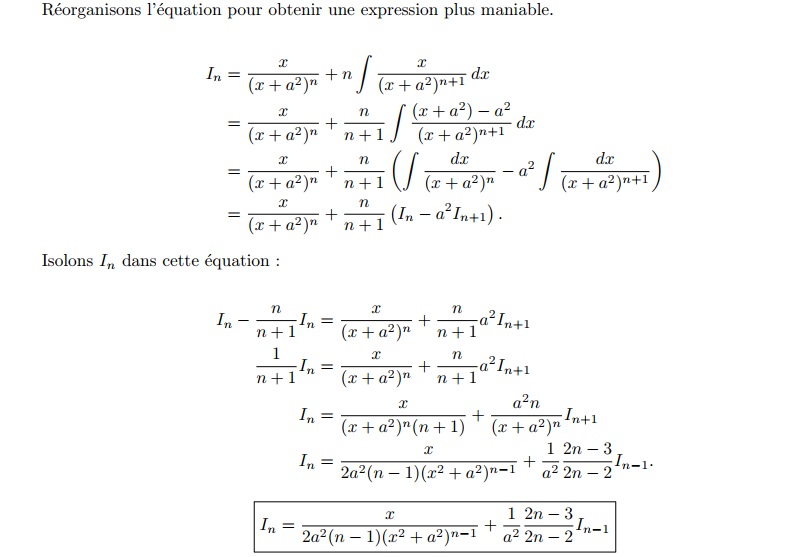
\includegraphics[width=0.6\textwidth]{images/calcul_integral/calcint-039-000.png}
\captionof{figure}{\small Régime transitoire RC : évolution de la tension $u_C(t)$ et du courant $i(t)$ lors de la charge et de la décharge.}
\end{center}
\begin{center}

\includegraphics[width=0.6\textwidth]{images/calcul_integral/calcint-039-001.png}
\captionof{figure}{\small Décroissance exponentielle de l'énergie $E(t)$ stockée dans le condensateur au cours de la décharge.}
\end{center}

\ifdefined\inMainDoc\else\end{document}\fi


% ================================================================
%  UE 6 : ÉLECTROCINÉTIQUE
% ================================================================
\newpage
\thispagestyle{empty}
\begin{tikzpicture}[remember picture, overlay]
  \fill[gray!12] ([xshift=1.5cm, yshift=3cm]current page.south west)
    rectangle ([xshift=-1.5cm, yshift=-3cm]current page.north east);
  \draw[line width=3pt] ([xshift=1.5cm,yshift=-3cm]current page.north west)
    -- ([xshift=-1.5cm,yshift=-3cm]current page.north east);
  \draw[line width=3pt] ([xshift=1.5cm,yshift=3cm]current page.south west)
    -- ([xshift=-1.5cm,yshift=3cm]current page.south east);
  \node[align=center] at (current page.center) {%
    {\fontsize{32}{40}\bfseries\selectfont ÉLECTROCINÉTIQUE}\\[0.4cm]
    {\fontsize{22}{28}\bfseries\selectfont ET RÉGIME VARIABLE}\\[1.2cm]
    {\large\itshape Circuits résistifs - Théorèmes de Thévenin et Norton}\\[0.4cm]
    {\large\itshape Régime sinusoïdal}\\[1.8cm]
    {\normalsize Licence 1 - UE 6}
  };
  \node[anchor=south west] at ([xshift=2cm,yshift=2cm]current page.south west)
    {\large\bfseries UE 6};
\end{tikzpicture}
\newpage

\addcontentsline{toc}{section}{ÉLECTROCINÉTIQUE ET RÉGIME VARIABLE}
\ifdefined\inMainDoc\else
\documentclass[12pt,a4paper]{article}
% ================================================================
%  PRÉAMBULE COMMUN - ANNALES CORRIGÉES
%  Université de Kara - FaST - Licence Fondamentale MPC
%  Design optimisé impression noir et blanc
% ================================================================

% -- ENCODAGE & LANGUE --
\usepackage[utf8]{inputenc}
\usepackage[T1]{fontenc}
\usepackage[french]{babel}
\usepackage{lmodern}
\usepackage{microtype}

% -- MISE EN PAGE --
\usepackage[a4paper, top=2.8cm, bottom=2.5cm, left=2.5cm, right=2.5cm, headheight=14pt]{geometry}
\usepackage{setspace}
\setstretch{1.2}
\usepackage{parskip}
\setlength{\parindent}{1.2em}
\setlength{\parskip}{4pt}

% -- MATHS --
\usepackage{amsmath, amssymb, mathtools, amsthm}
\usepackage{mathrsfs}
\usepackage{dsfont}
\usepackage{bm}
\usepackage{cancel}
\usepackage{textcomp}
% Définition de \oiint (intégrale de surface fermée) sans package supplémentaire
\newcommand{\oiint}{\mathop{\iint\!\!\!\!\!\!\!\bigcirc}\limits}

% -- PHYSIQUE & CHIMIE --
\usepackage{physics}
\usepackage{siunitx}
% Lorsque physics est chargé, siunitx omet \qty. On le restaure ici :
\AtBeginDocument{\RenewCommandCopy\qty\SI}
\sisetup{locale = FR, detect-all, output-decimal-marker={,}}
% Commande de substitution pour les unités posant problème avec pdflatex
% (ohm, degreeCelsius, micro, angstrom, percent utilisent des caractères non-ASCII)
\newcommand{\qtyohm}[1]{\ensuremath{\num{#1}\,\Omega}}
\newcommand{\qtydegc}[1]{\ensuremath{\num{#1}\,{}^\circ\text{C}}}
\newcommand{\qtyangstrom}[1]{\ensuremath{\num{#1}\,\text{\AA}}}
\newcommand{\qtypercent}[1]{\ensuremath{\num{#1}\,\%}}
\newcommand{\qtyum}[1]{\ensuremath{\num{#1}\,\mu\text{m}}}
\usepackage[version=4]{mhchem}

% -- GRAPHISMES --
\usepackage{graphicx}
\usepackage{float}
\usepackage{caption}
\usepackage{subcaption}
\usepackage{wrapfig}
\usepackage{tikz}
\usetikzlibrary{calc, arrows.meta, patterns, shapes.geometric}
\usepackage{pgfplots}
\pgfplotsset{compat=1.18}

% -- TABLEAUX --
\usepackage{booktabs}
\usepackage{array}
\usepackage{tabularx}
\usepackage{multirow}

% -- LISTES --
\usepackage{enumitem}
\setlist[enumerate]{topsep=3pt, itemsep=2pt, parsep=0pt}
\setlist[itemize]{topsep=3pt, itemsep=2pt, parsep=0pt, label={.}}

% -- BOÎTES (noir et blanc) --
\usepackage{mdframed}
\usepackage{tcolorbox}
\tcbuselibrary{skins, breakable, theorems}

% Boîte EXERCICE : encadré avec filet épais, fond blanc
\newmdenv[
  linewidth=1.2pt,
  linecolor=black,
  roundcorner=3pt,
  skipabove=10pt,
  skipbelow=6pt,
  innertopmargin=8pt,
  innerbottommargin=8pt,
  innerleftmargin=10pt,
  innerrightmargin=10pt,
  backgroundcolor=white,
  frametitle={\bfseries\small Exercice},
  frametitlealignment=\raggedright,
  frametitleaboveskip=4pt,
  frametitlebelowskip=4pt,
]{boiteexercice}

% Boîte CORRIGÉ : fond gris très clair + filet fin
\newmdenv[
  linewidth=0.6pt,
  linecolor=black,
  leftline=true,
  rightline=false,
  topline=false,
  bottomline=false,
  linecolor=black,
  innerleftmargin=12pt,
  innerrightmargin=8pt,
  innertopmargin=6pt,
  innerbottommargin=6pt,
  backgroundcolor=gray!8,
  skipabove=4pt,
  skipbelow=8pt,
]{boitecorrige}

% Boîte RÉSUMÉ DE COURS : double encadré
\newmdenv[
  linewidth=0.8pt,
  linecolor=black,
  roundcorner=2pt,
  backgroundcolor=gray!12,
  innertopmargin=10pt,
  innerbottommargin=10pt,
  innerleftmargin=12pt,
  innerrightmargin=12pt,
  skipabove=12pt,
  skipbelow=8pt,
]{boiteresume}

% Boîte ATTENTION/REMARQUE : barre gauche épaisse
\newmdenv[
  leftline=true,
  rightline=false,
  topline=false,
  bottomline=false,
  linewidth=3pt,
  linecolor=black,
  backgroundcolor=gray!5,
  innerleftmargin=12pt,
  innerrightmargin=8pt,
  innertopmargin=5pt,
  innerbottommargin=5pt,
  skipabove=6pt,
  skipbelow=6pt,
]{boiteremarque}

% -- DIFFICULTÉ DES EXERCICES --
\newcommand{\facile}{$\star$}
\newcommand{\moyen}{$\star\!\star$}
\newcommand{\difficile}{$\star\!\star\!\star$}
\newcommand{\niveau}[1]{\hfill\textbf{#1}\hspace{2pt}}

% -- EN-TÊTES ET PIEDS DE PAGE --
\usepackage{fancyhdr}
\pagestyle{fancy}
\fancyhf{}
\renewcommand{\headrulewidth}{0.5pt}
\renewcommand{\footrulewidth}{0.3pt}

% -- HYPERLIENS --
\usepackage[hidelinks]{hyperref}
\hypersetup{
    colorlinks=false,
    pdftitle={Annale Corrigée - Licence MPC - Université de Kara}
}

% -- TITRES --
\usepackage{titlesec}
\titleformat{\section}{\Large\bfseries}{\thesection.}{0.8em}{}[\vspace{2pt}\hrule\vspace{4pt}]
\titleformat{\subsection}{\large\bfseries}{\thesubsection.}{0.7em}{}
\titleformat{\subsubsection}{\normalsize\bfseries}{\thesubsubsection.}{0.6em}{}

% -- THÉORÈMES --
\theoremstyle{definition}
\newtheorem{defn}{Définition}[section]
\newtheorem{prop}{Propriété}[section]
\newtheorem{thm}{Théorème}[section]
\newtheorem{corol}{Corollaire}[section]
\newtheorem{exemple}{Exemple}[section]

% -- COMMANDES MATHÉMATIQUES UTILES --
\newcommand{\vect}[1]{\overrightarrow{#1}}
\newcommand{\R}{\mathbb{R}}
\newcommand{\N}{\mathbb{N}}
\newcommand{\Z}{\mathbb{Z}}
\newcommand{\C}{\mathbb{C}}
\renewcommand{\d}{\mathrm{d}}
\newcommand{\deriv}[2]{\dfrac{\d #1}{\d #2}}
\newcommand{\dpart}[2]{\dfrac{\partial #1}{\partial #2}}
\newcommand{\rot}{\overrightarrow{\mathrm{rot}}\,}
\renewcommand{\div}{\mathrm{div}\,}
\renewcommand{\grad}{\overrightarrow{\mathrm{grad}}\,}
\newcommand{\e}{\mathrm{e}}
\newcommand{\ii}{\mathrm{i}}
\renewcommand{\Tr}{\mathrm{Tr}}

% Numérotation des équations par section
\numberwithin{equation}{section}

% -- RÉSULTATS ENCADRÉS --
\newcommand{\res}[1]{\[\boxed{#1}\]}

% -- REMARQUE INLINE --
\newcommand{\rmq}[1]{\begin{boiteremarque}\textbf{Remarque.} #1\end{boiteremarque}}

% -- MISE EN VALEUR DU RÉSULTAT FINAL --
\newcommand{\reponse}[1]{%
  \begin{center}
    \fbox{\begin{minipage}{0.92\textwidth}\centering #1\end{minipage}}
  \end{center}%
}


\lhead{\small\textit{Électrocinétique - Licence 1}}
\rhead{\small\textit{FaST, Université de Kara}}
\cfoot{\thepage}

\begin{document}
\fi

\begin{center}
  {\LARGE\bfseries ÉLECTROCINÉTIQUE ET RÉGIME VARIABLE}\\[0.3cm]
  {\normalsize Licence 1 - Mathématiques, Physique et Chimie}\\[0.1cm]
  \rule{0.7\textwidth}{0.8pt}
\end{center}

\vspace{0.3cm}

% ================================================================
\section*{Résumé du cours}
% ================================================================

\begin{boiteresume}

\textbf{1. Lois fondamentales.}
\begin{itemize}[nosep]
  \item \textbf{Loi des n\oe{}uds (Kirchhoff courant)} : la somme algébrique des courants entrant en un n\oe{}ud est nulle : $\sum I_k = 0$.
  \item \textbf{Loi des mailles (Kirchhoff tension)} : la somme algébrique des tensions le long d'une maille fermée est nulle : $\sum U_k = 0$.
  \item \textbf{Loi d'Ohm} (convention récepteur) : $U = RI$.
\end{itemize}

\textbf{2. Associations de résistances.}
\begin{itemize}[nosep]
  \item En série : $R_{eq} = R_1 + R_2 + \cdots$
  \item En parallèle : $\dfrac{1}{R_{eq}} = \dfrac{1}{R_1} + \dfrac{1}{R_2} + \cdots$
\end{itemize}

\textbf{3. Diviseur de tension et diviseur de courant.}
\[
U_{R_2} = \frac{R_2}{R_1 + R_2}\,E \qquad I_{R_2} = \frac{G_2}{G_1 + G_2}\,I = \frac{R_1}{R_1 + R_2}\,I
\]
(avec $G_k = 1/R_k$ la conductance).

\textbf{4. Théorèmes de Thévenin et Norton.}
\begin{itemize}[nosep]
  \item \textbf{Thévenin} : tout circuit linéaire vu de deux bornes A, B est équivalent à une source de tension $E_{th}$ (tension à vide entre A et B) en série avec $R_{th}$ (résistance vue des bornes avec les sources éteintes).
  \item \textbf{Norton} : équivalent de Thévenin $\to$ Norton via $I_N = E_{th}/R_{th}$, résistance identique $R_{th}$.
\end{itemize}

\textbf{5. Théorème de Millman.}
Pour $n$ branches en parallèle entre les n\oe{}uds A et B :
\[
U_{AB} = \frac{\displaystyle\sum_{k=1}^{n} \frac{\varepsilon_k}{R_k}}{\displaystyle\sum_{k=1}^{n} \frac{1}{R_k}}
\]
où $\varepsilon_k$ est la f.é.m. de la $k$-ième branche (comptée positivement si elle pousse de B vers A).

\textbf{6. Puissance transmise à une charge.} La puissance maximale est transmise à une charge $R_L$ lorsque $R_L = R_{th}$ (condition d'adaptation d'impédance) :
\[
P_{\max} = \frac{E_{th}^2}{4R_{th}}
\]

\end{boiteresume}

\newpage

% ================================================================
\section{Circuits résistifs et théorèmes}
% ================================================================

\subsection*{Exercice 1 - Réseau à deux mailles \niveau{\moyen}}

\begin{boiteexercice}
\begin{minipage}{0.6\textwidth}
Déterminer, pour le circuit ci-contre, l'intensité $i$ traversant $R_2$ et la tension $u$ aux bornes de $R_3$ :
\begin{enumerate}
  \item en faisant des associations de résistances et en appliquant le diviseur de tension ;
  \item en faisant une transformation Thévenin $\to$ Norton et en appliquant le diviseur de courant.
  \item Application numérique : $E = \qty{6}{V}$, $R_1 = \qtyohm{100}$, $R_2 = R_3 = R_4 = \qtyohm{50}$.
\end{enumerate}
\end{minipage}
\hfill
\begin{minipage}{0.35\textwidth}
\centering
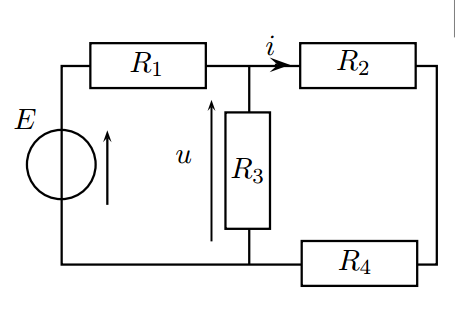
\includegraphics[width=\textwidth]{images/el2.png}
\end{minipage}
\end{boiteexercice}

\begin{boitecorrige}
\textbf{1. Méthode par associations.}

$R_2$ et $R_4$ sont en série : $R_5 = R_2 + R_4$.

$R_3$ et $R_5$ sont en parallèle :
\[
R_6 = \frac{R_3 R_5}{R_3 + R_5}
\]
$R_1$ et $R_6$ sont en série, soumis à $E$. La tension $u = U_{AB}$ est donnée par le diviseur de tension :
\[
\boxed{u = U_{AB} = \frac{R_3(R_2+R_4)}{R_1 R_3 + (R_1+R_3)(R_2+R_4)}\,E}
\]
Le courant dans $R_5$ (donc dans $R_2$) :
\[
\boxed{i = \frac{u}{R_5} = \frac{R_3\,E}{R_1 R_3 + (R_1+R_3)(R_2+R_4)}}
\]

\begin{boiteremarque}
$i$ n'apparaît plus dans le schéma simplifié final. Il faut revenir au schéma intermédiaire (avant la mise en parallèle de $R_3$ et $R_5$) pour l'exprimer.
\end{boiteremarque}

\textbf{2. Transformation Thévenin $\to$ Norton.}

Entre les n\oe{}uds A et B, on a un générateur de Thévenin ($E$, $R_1$). Transformation en Norton : $\eta = E/R_1$, résistance équivalente $R_0 = R_1 R_3/(R_1 + R_3)$ (après mise en parallèle de $R_1$ et $R_3$). Le diviseur de courant donne le même résultat qu'à la question 1.

\textbf{3. Application numérique :} $R_5 = 100\,\Omega$, $R_6 = R_3 R_5/(R_3+R_5) = 50\times100/150 \approx 33{,}3\,\Omega$.
\[
u = \frac{33{,}3}{100+33{,}3}\times 6 \approx \qty{1.5}{V} \qquad i = \frac{1{,}5}{100} = \qty{15}{mA}
\]
\end{boitecorrige}

\begin{center}
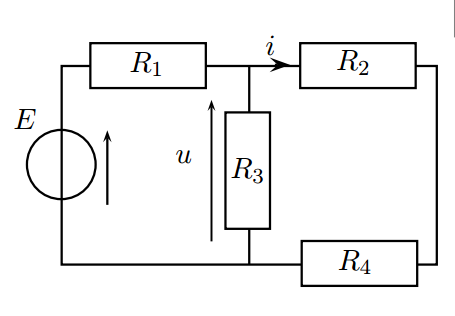
\includegraphics[width=0.6\textwidth]{images/electrocinetique/elec-001-000.png}
\captionof{figure}{\small Schéma du réseau à deux mailles avec courants et tensions.}
\end{center}
\begin{center}

\includegraphics[width=0.6\textwidth]{images/electrocinetique/elec-001-001.png}
\captionof{figure}{\small Application des lois de Kirchhoff au réseau.}
\end{center}

\subsection*{Exercice 2 - Circuit linéaire \niveau{\moyen}}

\begin{boiteexercice}
\begin{minipage}{0.6\textwidth}
Dans le circuit ci-contre, avec $R = \qtyohm{1}$, $E = \qty{5}{V}$, $E' = \qty{3}{V}$ :
\begin{enumerate}
  \item Calculer $U_{EF}$.
  \item Calculer $I_0$ dans la branche principale.
  \item Calculer $I'$ dans la branche contenant $E'$.
  \item Calculer $i_1$, $i_2$ et $i_3$.
\end{enumerate}
\end{minipage}
\hfill
\begin{minipage}{0.35\textwidth}
\centering
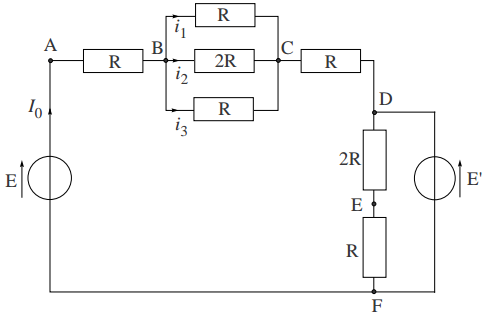
\includegraphics[width=\textwidth]{images/el7.png}
\end{minipage}
\end{boiteexercice}

\begin{boitecorrige}
\textbf{1.} La branche $\{D,\,2R,\,R,\,F\}$ constitue un diviseur de tension soumis à $E'$ :
\[
\boxed{U_{EF} = \frac{R}{R + 2R}\,E' = \frac{1}{3}\times3 = \qty{1}{V}}
\]

\textbf{2.} La résistance équivalente entre B et C est :
\[
R_{eq} = (R \parallel R) \parallel 2R = \frac{R}{2} \parallel 2R = \frac{\frac{R}{2}\times 2R}{\frac{R}{2}+2R} = \frac{R^2}{\frac{5R}{2}} = \frac{2R}{5}
\]
La branche $\{D, 2R, R, F\}$ est en parallèle avec $E'$ qui impose la tension à ses bornes. Du point de vue de la branche principale, les deux f.é.m. $E$ et $E'$ s'opposent (en série, sens contraires) ; la f.é.m. résultante est $E_0 = E - E' = \qty{2}{V}$.

La résistance totale de la maille principale est $R_0 = R + R_{eq} + R = R + \frac{2R}{5} + R = \frac{12R}{5} = \frac{12}{5}\,\Omega$.
\[
\boxed{I_0 = \frac{E_0}{R_0} = \frac{E-E'}{R_0} = \frac{2}{\frac{12}{5}} = \frac{5}{6}\,\text{A} \approx \qty{0.83}{A}}
\]

\textbf{3.} Le courant $I''$ circulant de D vers F dans la branche contenant $3R$ (soumise à $E'$) est, en convention récepteur :
\[
I'' = \frac{E'}{3R} = \frac{3}{3\times1} = \qty{1}{A}
\]
En définissant $I'$ en convention générateur par rapport à $E'$ (sens F $\to$ D dans $E'$), la loi des n\oe{}uds en D donne :
\[
\boxed{I' = I'' - I_0 = 1 - \frac{5}{6} = \frac{1}{6}\,\text{A} \approx \qty{0.17}{A} \quad (\text{de F vers D})}
\]

\textbf{4.} Par symétrie du réseau entre B et C : $i_1 = i_3$. Diviseur de courant en B :
\[
\boxed{i_1 = i_3 = \frac{R_{eq}}{R}\,I_0 = \frac{2R/5}{R}\,I_0 = \frac{2}{5}\times\frac{5}{6} = \frac{1}{3}\,\text{A} \approx \qty{0.33}{A}}
\]
\[
\boxed{i_2 = \frac{R_{eq}}{2R}\,I_0 = \frac{2R/5}{2R}\,I_0 = \frac{1}{5}\times\frac{5}{6} = \frac{1}{6}\,\text{A} \approx \qty{0.17}{A}}
\]
Vérification : $I_0 = i_1 + i_2 + i_3 = \frac{1}{3}+\frac{1}{6}+\frac{1}{3} = \frac{5}{6}$. Correct.
\end{boitecorrige}

\begin{center}
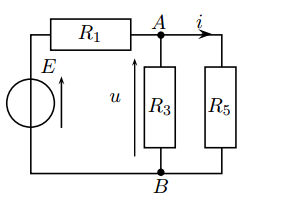
\includegraphics[width=0.5\textwidth]{images/electrocinetique/elec-002-006.png}
\captionof{figure}{\small Circuit linéaire : schéma avec sources et résistances.}
\end{center}
\begin{center}

\includegraphics[width=0.5\textwidth]{images/electrocinetique/elec-002-007.png}
\captionof{figure}{\small Analyse du circuit par les lois de Kirchhoff.}
\end{center}

\subsection*{Exercice 3 - Théorème de Thévenin \niveau{\moyen}}

\begin{boiteexercice}
\begin{center}
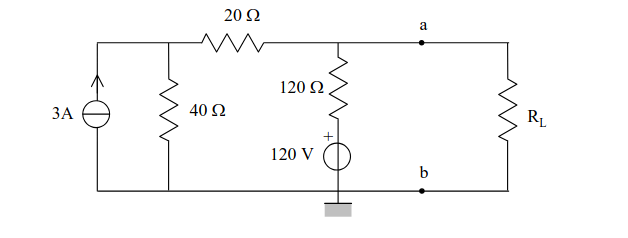
\includegraphics[width=0.7\textwidth]{images/el20.png}
\end{center}
$R_L$ est la résistance de charge.
\begin{enumerate}
  \item Déterminer le circuit équivalent de Thévenin vu entre les points a et b.
  \item Quelle valeur de $R_L$ permet de transmettre la puissance maximale à la charge ? Calculer cette puissance.
  \item Calculer la puissance transmise si $R_L = 2R_{th}$.
\end{enumerate}
\end{boiteexercice}

\begin{boitecorrige}
\textbf{1.} Par le calcul (tensions à vide et court-circuit) :
\[
E_{th} = \qty{120}{V} \qquad R_{th} = \qtyohm{40}
\]

\textbf{2.} La condition d'adaptation d'impédance donne la puissance maximale pour $R_L = R_{th}$ :
\[
\boxed{R_L = R_{th} = \qtyohm{40}}
\]
\[
P_{\max} = R_L\left(\frac{E_{th}}{R_L + R_{th}}\right)^2 = 40\times\left(\frac{120}{80}\right)^2 = 40\times2{,}25 = \qty{90}{W}
\]

\textbf{3.} Pour $R_L = 2R_{th} = \qtyohm{80}$ :
\[
P = 80\times\left(\frac{120}{80+40}\right)^2 = 80\times\left(\frac{120}{120}\right)^2 = 80\times1 = \qty{80}{W}
\]
\end{boitecorrige}

\subsection*{Exercice 4 - Théorème de Millman \niveau{\moyen}}

\begin{boiteexercice}
\begin{center}
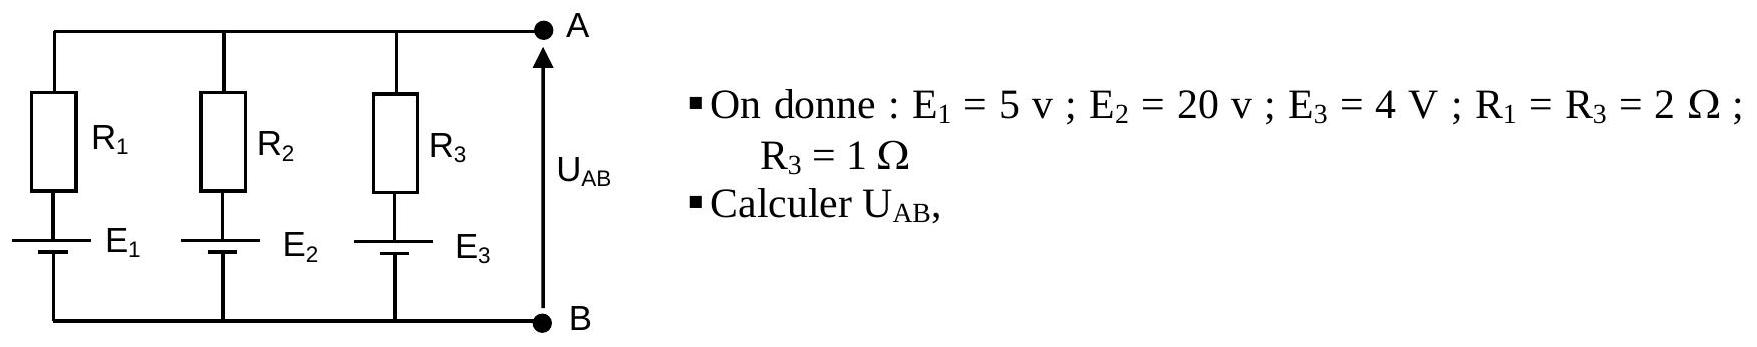
\includegraphics[width=0.85\textwidth]{images/el23.png}
\end{center}
\begin{enumerate}
  \item Calculer $U_{AB}$ en utilisant le théorème de Millman.
  \item Déterminer le courant $I$ traversant $R_4$.
\end{enumerate}
\end{boiteexercice}

\begin{boitecorrige}
\textbf{1.} On applique le théorème de Millman entre les n\oe{}uds A et B. Les trois branches en parallèle contiennent respectivement les f.é.m. $E_1 = \qty{4}{V}$ (sens B$\to$A), $E_2 = \qty{5}{V}$ (sens A$\to$B), $E_3 = \qty{8}{V}$ (sens B$\to$A), avec $R_1 = \qtyohm{2}$, $R_2 = \qtyohm{1}$, $R_3 = \qtyohm{2}$ :
\[
U_{AB} = \frac{-\dfrac{E_1}{R_1}+\dfrac{E_2}{R_2}-\dfrac{E_3}{R_3}}{\dfrac{1}{R_1}+\dfrac{1}{R_2}+\dfrac{1}{R_3}} = \frac{-\dfrac{4}{2}+\dfrac{5}{1}-\dfrac{8}{2}}{\dfrac{1}{2}+\dfrac{1}{1}+\dfrac{1}{2}} = \frac{-2+5-4}{0{,}5+1+0{,}5} = \frac{-1}{2} = \qty{-0.5}{V}
\]

\begin{boiteremarque}
Le signe de chaque f.é.m. dans Millman dépend de son sens par rapport au sens de référence A$\to$B. Une f.é.m. qui pousse dans le sens A$\to$B est positive, dans le sens B$\to$A est négative.
\end{boiteremarque}

\textbf{2.} Par l'équivalent de Thévenin avec $E_{th} = U_{AB}$ et $R_{th} = R_1\parallel R_2\parallel R_3 = \qtyohm{0.5}$ :
\[
I = \frac{E_{th}}{R_{th}+R_4} = \frac{0{,}5}{0{,}5 + R_4}
\]
(voir figure el24.png pour la valeur numérique de $R_4$).
\end{boitecorrige}

\begin{center}
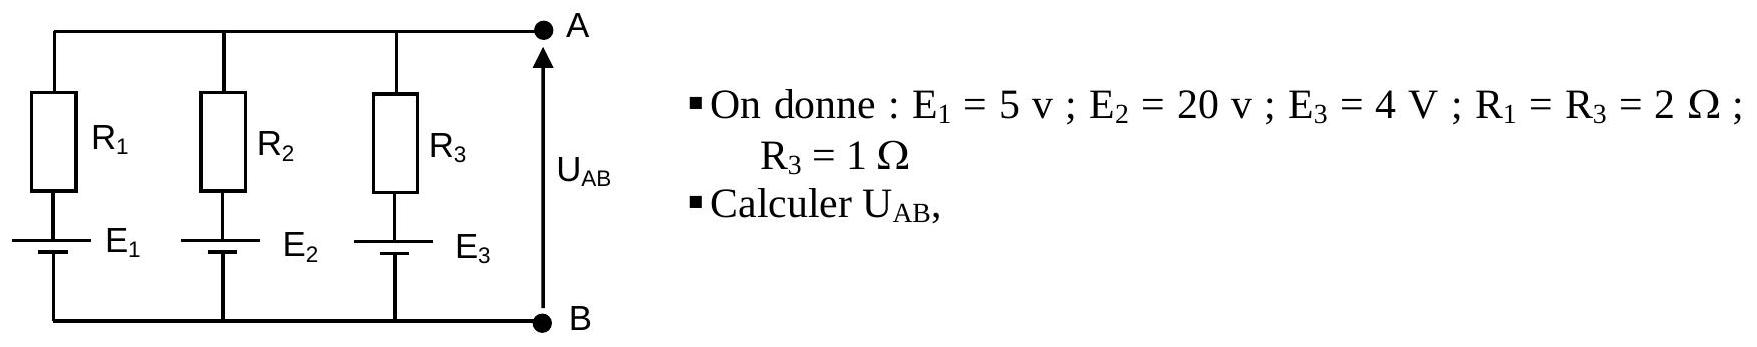
\includegraphics[width=0.7\textwidth]{images/electrocinetique/elec-004-014.png}
\captionof{figure}{\small Théorème de Millman : application à un n\oe{}ud à plusieurs branches.}
\end{center}

\subsection*{Exercice 5 - Théorème de Norton \niveau{\facile}}

\begin{boiteexercice}
Déterminer les modèles équivalents de Norton des circuits placés à gauche de AB dans chacun des schémas suivants.

\begin{minipage}{0.48\textwidth}
\centering
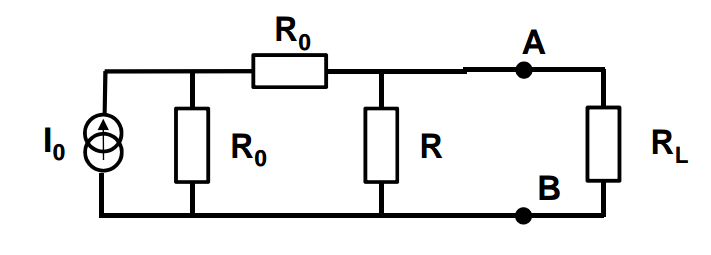
\includegraphics[width=\textwidth]{images/el31.png}
\end{minipage}
\hfill
\begin{minipage}{0.48\textwidth}
\centering
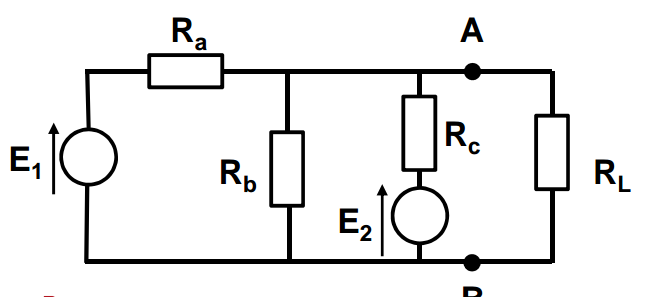
\includegraphics[width=\textwidth]{images/el32.png}
\end{minipage}
\end{boiteexercice}

\begin{boitecorrige}
\textbf{Schéma 1 :} Le courant de court-circuit $I_{AB}$ (obtenu en court-circuitant A et B) est la moitié du courant source : $I_{AB} = I_0/2$. La résistance équivalente (source de courant éteinte, c.-à-d. ouverte) est $R_{AB} = R \parallel 2R_0$.

\textbf{Schéma 2 :} Le courant de court-circuit (source de tension $E_1$ en série avec $R_a$, bornes AB court-circuitées) donne $I_{AB} = E_1/R_a$. La résistance équivalente (source $E_1$ éteinte) : $R_{AB} = R_a \parallel R_b \parallel R_c$.
\end{boitecorrige}

\begin{center}
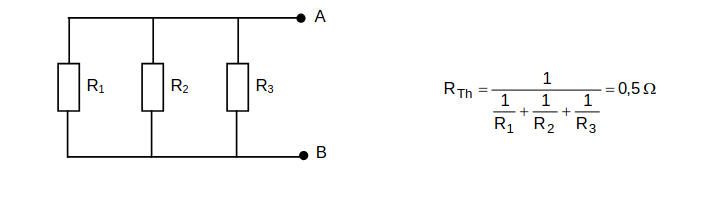
\includegraphics[width=0.6\textwidth]{images/electrocinetique/elec-005-015.png}
\captionof{figure}{\small Modèle équivalent de Norton : source de courant en parallèle avec une résistance.}
\end{center}
\begin{center}

\includegraphics[width=0.6\textwidth]{images/electrocinetique/elec-005-016.png}
\captionof{figure}{\small Transformation Norton $\leftrightarrow$ Thévenin : équivalence des modèles.}
\end{center}
\begin{center}
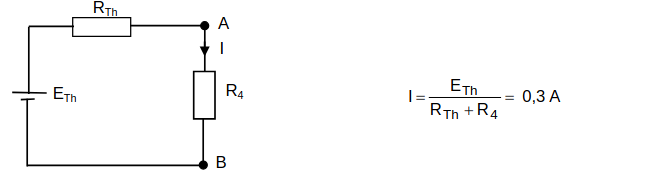
\includegraphics[width=0.6\textwidth]{images/electrocinetique/elec-005-017.png}
\captionof{figure}{\small Calcul du courant de court-circuit $I_{AB}$ pour le schéma 1.}
\end{center}
\begin{center}

\includegraphics[width=0.6\textwidth]{images/electrocinetique/elec-005-018.png}
\captionof{figure}{\small Calcul de la résistance équivalente $R_{AB}$ pour le schéma 2.}
\end{center}

\subsection*{Exercice 6 - Circuits en régime sinusoïdal \niveau{\difficile}}

\begin{boiteexercice}
\begin{center}
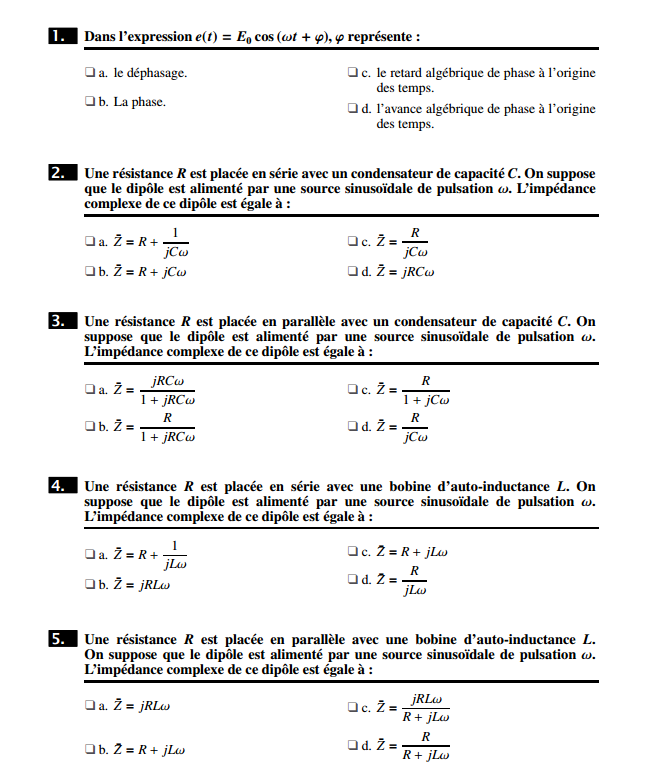
\includegraphics[width=0.65\textwidth]{images/el27.png}
\end{center}
\begin{center}
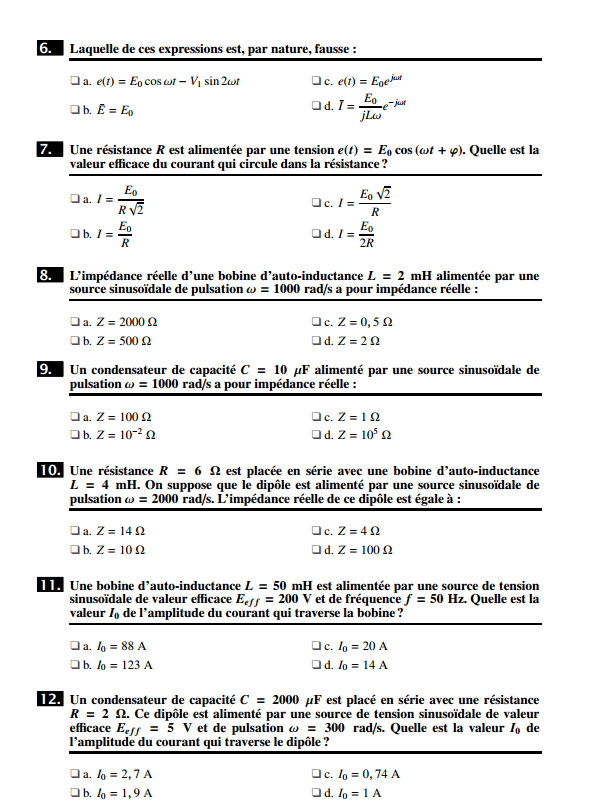
\includegraphics[width=0.65\textwidth]{images/el28.png}
\end{center}
Répondre aux questions posées sur les figures.
\end{boiteexercice}

\clearpage
\begin{boitecorrige}
\begin{center}
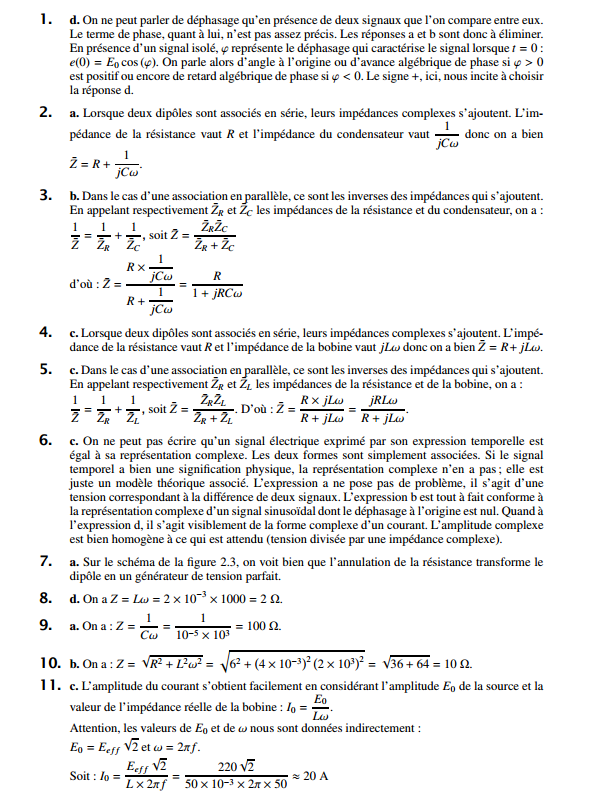
\includegraphics[width=0.7\textwidth]{images/el29.png}
\end{center}
\begin{center}
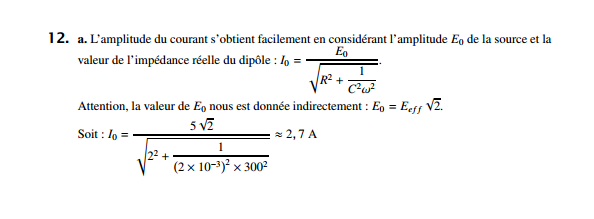
\includegraphics[width=0.7\textwidth]{images/el30.png}
\end{center}
\end{boitecorrige}

\begin{center}
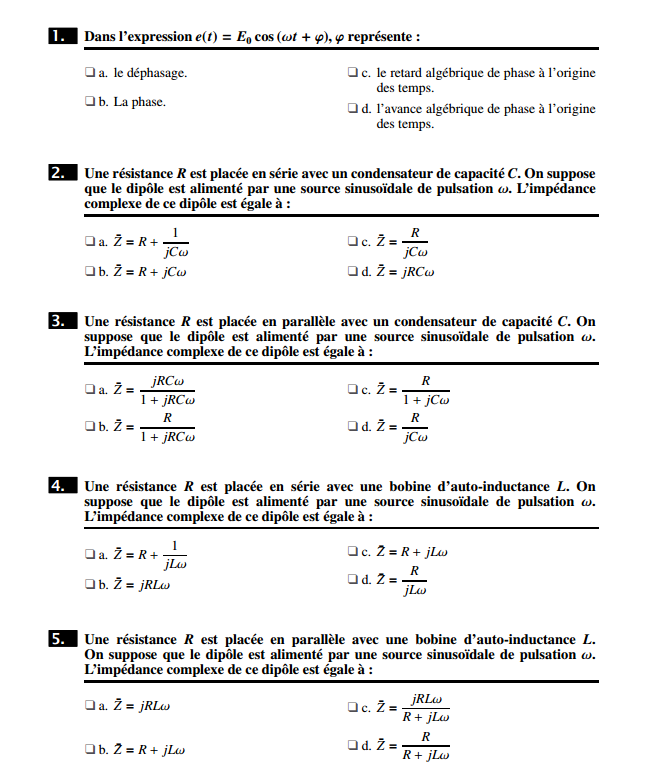
\includegraphics[height=0.5\textheight]{images/electrocinetique/elec-006-023.png}
\captionof{figure}{\small Circuit en régime sinusoïdal : représentation complexe des impédances.}
\end{center}
\begin{center}

\includegraphics[height=0.5\textheight]{images/electrocinetique/elec-006-024.png}
\captionof{figure}{\small Diagramme de Fresnel des tensions et courants en régime sinusoïdal.}
\end{center}

\section{Régimes transitoires}

\subsection*{Exercice 7 - Circuit RC : charge et décharge \niveau{\moyen}}

\begin{boiteexercice}
\begin{center}
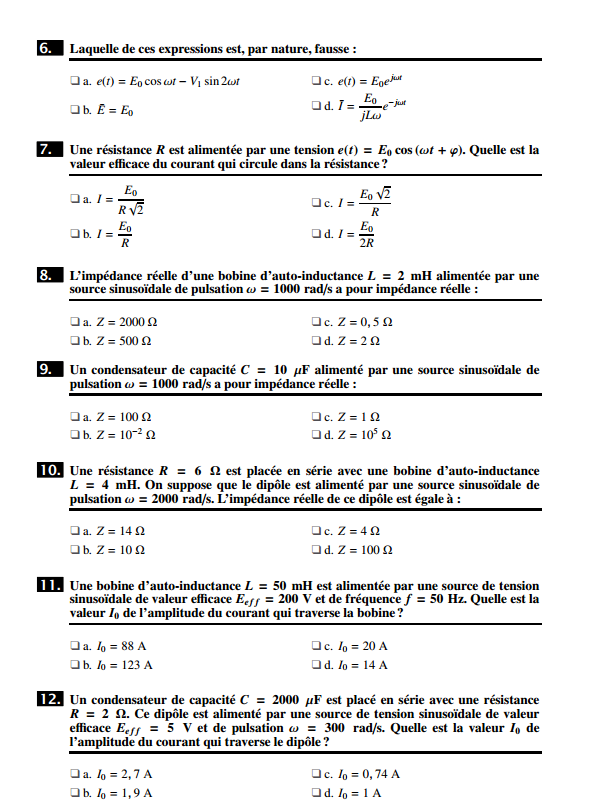
\includegraphics[height=0.45\textheight]{images/electrocinetique/elec-007-025.png}
\captionof{figure}{\small Circuit RC : charge et décharge d'un condensateur à travers une résistance.}
\end{center}
Un condensateur $C = \qty{10}{\mu F}$ est initialement déchargé. On le charge à travers $R = \qty{100}{k\Omega}$ par un générateur de f.é.m. $E = \qty{12}{V}$.
\begin{enumerate}
  \item Écrire l'équation différentielle régissant la tension $u_C(t)$ aux bornes du condensateur.
  \item Résoudre et tracer qualitativement $u_C(t)$.
  \item Calculer la constante de temps $\tau$ et le temps pour atteindre $95\,\%$ de la charge finale.
  \item On ouvre le circuit quand $u_C = \qty{8}{V}$. La résistance de décharge est $R' = \qty{50}{k\Omega}$. Écrire et résoudre l'équation de décharge.
\end{enumerate}
\end{boiteexercice}

\begin{boitecorrige}
\textbf{1.} La loi des mailles donne : $E = Ri + u_C$ avec $i = C\,\d u_C/\d t$ :
\[
RC\,\frac{\d u_C}{\d t} + u_C = E
\]

\textbf{2.} L'équation homogène $RC\,\d u_C/\d t + u_C = 0$ a pour solution $u_C^{hom} = Ke^{-t/\tau}$ avec $\tau = RC$. Solution particulière $u_C^{part} = E$.
\[
u_C(t) = E(1-e^{-t/\tau}) \quad \text{avec } u_C(0)=0
\]

\textbf{3.} $\tau = RC = 10^5\times10^{-5} = \qty{1}{s}$.

$u_C(t_{95}) = 0{,}95E$ donne $1-e^{-t_{95}/\tau}=0{,}95$, soit $e^{-t_{95}}=0{,}05$, $t_{95} = -\ln(0{,}05) \approx 3\tau = \qty{3}{s}$.

\textbf{4.} La décharge part de $u_0=\qty{8}{V}$ avec constante $\tau' = R'C = 5\times10^4\times10^{-5} = \qty{0.5}{s}$ :
\[
u_C(t) = u_0\,e^{-t/\tau'} = 8e^{-2t} \quad [\text{V}], \quad t\geq0
\]
(l'origine du temps est remise à zéro au moment de l'ouverture).
\end{boitecorrige}

\subsection*{Exercice 8 - Circuit RL en régime transitoire \niveau{\moyen}}

\begin{boiteexercice}
\begin{center}
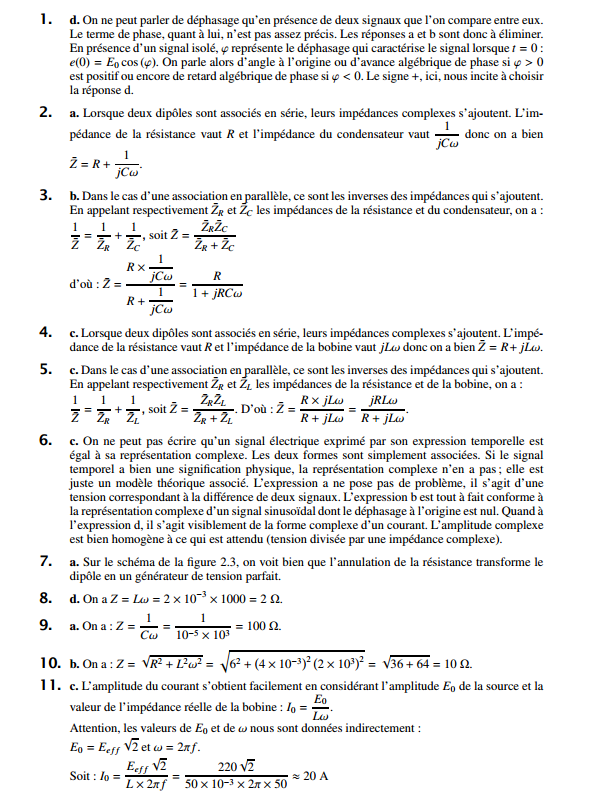
\includegraphics[height=0.45\textheight]{images/electrocinetique/elec-008-027.png}
\captionof{figure}{\small Circuit RL : établissement et rupture du courant dans une bobine.}
\end{center}
Un circuit RL série comporte $R = \qty{50}{\Omega}$ et $L = \qty{100}{mH}$. À $t=0$, on connecte une source de tension $E = \qty{10}{V}$.
\begin{enumerate}
  \item Écrire l'équation différentielle du courant $i(t)$.
  \item Trouver $i(t)$ sachant que $i(0) = 0$.
  \item Calculer $\tau$, $i_{max}$ et le courant à $t=\tau$.
  \item Calculer l'énergie stockée dans l'inductance en régime permanent.
\end{enumerate}
\end{boiteexercice}

\begin{boitecorrige}
\textbf{1.} Loi des mailles :
\[
L\frac{\d i}{\d t}+Ri = E
\]

\textbf{2.} Séparation homogène + particulière :
\[
i(t) = \frac{E}{R}\left(1-e^{-t/\tau}\right) \quad \text{avec}\quad \tau=\frac{L}{R}
\]

\textbf{3.} $\tau = L/R = 0{,}1/50 = \qty{2}{ms}$. $i_{max} = E/R = 10/50 = \qty{200}{mA}$.
$i(\tau) = i_{max}(1-e^{-1}) = 0{,}2\times(1-0{,}368) \approx \qty{126}{mA} \approx 63{,}2\,\%$ de $i_{max}$.

\textbf{4.} En régime permanent, $i = i_{max} = \qty{200}{mA}$ :
\[
W_L = \frac{1}{2}Li_{max}^2 = \frac{1}{2}\times0{,}1\times(0{,}2)^2 = \qty{2}{mJ}
\]
\end{boitecorrige}

\section{Régime sinusoïdal forcé}

\subsection*{Exercice 9 - Impédance complexe \niveau{\moyen}}

\begin{boiteexercice}
Un circuit RLC série est alimenté par $e(t) = E_0\cos(\omega t)$ avec $E_0 = \qty{10}{V}$, $R = \qty{10}{\Omega}$, $L = \qty{100}{mH}$, $C = \qty{100}{\mu F}$, $\omega = \qty{200}{rad.s^{-1}}$.
\begin{enumerate}
  \item Calculer les impédances $Z_R$, $Z_L$, $Z_C$ et l'impédance totale $Z$.
  \item Calculer l'intensité maximale $I_0$ et le déphasage $\varphi$ entre la tension et le courant.
  \item Calculer les tensions efficaces aux bornes de chaque élément.
  \item Exprimer $i(t)$ et $u_R(t)$.
\end{enumerate}
\end{boiteexercice}

\begin{boitecorrige}
\textbf{1.} $Z_R = R = \qty{10}{\Omega}$, $Z_L = j\omega L = j\times200\times0{,}1 = j\qty{20}{\Omega}$, $Z_C = \frac{1}{j\omega C} = \frac{1}{j\times200\times10^{-4}} = \frac{-j}{0{,}02} = -j\qty{50}{\Omega}$.
\[
Z = R+j\omega L+\frac{1}{j\omega C} = 10+j20-j50 = 10-j30 = \sqrt{10^2+30^2}\,\angle\arctan(-30/10)
\]
\[
|Z| = \sqrt{100+900} = \sqrt{1000} \approx \qty{31.6}{\Omega}, \quad \varphi = \arctan(-3) \approx -71{,}6^\circ 
\]

\textbf{2.} $I_0 = E_0/|Z| = 10/31{,}6 \approx \qty{316}{mA}$. Le déphasage $\varphi\approx-71{,}6^\circ $ : le courant est en avance sur la tension (circuit capacitif).

\textbf{3.} Valeurs efficaces : $U_R = RI_{eff} = 10\times0{,}316/\sqrt{2} \approx \qty{2.24}{V}$, $U_L = \omega L\cdot I_{eff} = 20\times\qty{0.224}{A} \approx \qty{4.47}{V}$, $U_C = I_{eff}/(\omega C) = 50\times\qty{0.224}{A} \approx \qty{11.2}{V}$.

\textbf{4.}
\[
i(t) = I_0\cos(\omega t-\varphi) = 0{,}316\cos(200t+71{,}6^\circ ) \quad [\text{A}]
\]
\[
u_R(t) = Ri(t) = 3{,}16\cos(200t+71{,}6^\circ ) \quad [\text{V}]
\]
\end{boitecorrige}

\subsection*{Exercice 10 - Résonance en série \niveau{\difficile}}

\begin{boiteexercice}
Reprendre le circuit RLC série de l'exercice précédent.
\begin{enumerate}
  \item À quelle pulsation $\omega_0$ se produit la résonance ? Calculer $\omega_0$.
  \item Quelle est la valeur maximale du courant à la résonance ?
  \item Définir et calculer le facteur de qualité $Q$.
  \item La bande passante $\Delta\omega$ est définie par les pulsations $\omega_\pm$ pour lesquelles $I = I_{max}/\sqrt{2}$. Calculer $\Delta\omega$.
\end{enumerate}
\end{boiteexercice}

\begin{boitecorrige}
\textbf{1.} La résonance se produit quand $\text{Im}(Z) = 0$, soit $\omega L = 1/(\omega C)$ :
\[
\omega_0 = \frac{1}{\sqrt{LC}} = \frac{1}{\sqrt{0{,}1\times10^{-4}}} = \frac{1}{\sqrt{10^{-5}}} = \frac{1}{10^{-5/2}} = 10^{5/2} \approx \qty{316}{rad.s^{-1}}
\]

\textbf{2.} À la résonance, $Z = R$ (l'inductance et le condensateur se compensent) :
\[
I_{max} = \frac{E_0}{R} = \frac{10}{10} = \qty{1}{A}
\]

\textbf{3.} Le facteur de qualité :
\[
Q = \frac{\omega_0 L}{R} = \frac{316\times0{,}1}{10} = \qty{3.16}{}
\]
Ou encore $Q = 1/(\omega_0 CR) = 1/(316\times10^{-4}\times10) \approx 3{,}16$.

\textbf{4.} La bande passante est $\Delta\omega = \omega_0/Q = 316/3{,}16 = \qty{100}{rad.s^{-1}}$.

Les pulsations de coupure à $-3\,\text{dB}$ : $\omega_\pm = \omega_0\pm\Delta\omega/2 = 316\pm50$, soit $\omega_+ = \qty{366}{rad.s^{-1}}$ et $\omega_- = \qty{266}{rad.s^{-1}}$.
\end{boitecorrige}

\subsection*{Exercice 11 - Filtres du premier ordre \niveau{\moyen}}

\begin{boiteexercice}
\begin{enumerate}
  \item On considère un filtre RC (résistance en série, condensateur en sortie). Montrer que la fonction de transfert est $H(j\omega) = \frac{1}{1+j\omega RC}$ et que c'est un filtre passe-bas.
  \item Calculer la fréquence de coupure $f_c$ pour $R = \qty{1}{k\Omega}$ et $C = \qty{1}{\mu F}$.
  \item Calculer le gain en dB et le déphasage à $f = f_c$, $f = f_c/10$ et $f = 10f_c$.
  \item Si on inverse $R$ et $C$ (condensateur en série, résistance en sortie), montrer que c'est un filtre passe-haut.
\end{enumerate}
\end{boiteexercice}

\begin{boitecorrige}
\textbf{1.} Par le diviseur de tension : $U_s = \frac{Z_C}{Z_R+Z_C}U_e = \frac{1/(j\omega C)}{R+1/(j\omega C)}U_e$.
\[
H(j\omega) = \frac{U_s}{U_e} = \frac{1}{1+j\omega RC}
\]
$|H| = 1/\sqrt{1+(\omega RC)^2}$ est une fonction décroissante de $\omega$ : c'est bien un \textbf{filtre passe-bas}.

\textbf{2.} La fréquence de coupure est définie par $|H(j\omega_c)| = 1/\sqrt{2}$ :
\[
\omega_c = \frac{1}{RC} = \frac{1}{10^3\times10^{-6}} = \qty{1000}{rad.s^{-1}}, \quad f_c = \frac{\omega_c}{2\pi} \approx \qty{159}{Hz}
\]

\textbf{3.}
\begin{center}
\begin{tabular}{lccc}
\toprule
$f$ & $|H|$ & Gain (dB) & $\varphi = -\arctan(\omega RC)$\\
\midrule
$f_c/10$ & $\approx1$ & $\approx0\,\text{dB}$ & $\approx -5{,}7^\circ $\\
$f_c$ & $1/\sqrt{2}$ & $-3\,\text{dB}$ & $-45^\circ $\\
$10f_c$ & $\approx0{,}1$ & $\approx-20\,\text{dB}$ & $\approx -84^\circ $\\
\bottomrule
\end{tabular}
\end{center}
Au-delà de $f_c$, le gain diminue de $-20\,\text{dB/décade}$ (pente du diagramme de Bode asymptotique).

\textbf{4.} En intervertissant : $U_s = \frac{R}{R+1/(j\omega C)}U_e = \frac{j\omega RC}{1+j\omega RC}U_e$.
$|H| = \omega RC/\sqrt{1+(\omega RC)^2}$ est croissante avec $\omega$ : \textbf{filtre passe-haut}.
\end{boitecorrige}

\subsection*{Exercice 12 - Puissance en régime sinusoïdal \niveau{\moyen}}

\begin{boiteexercice}
Un circuit RL est alimenté par une tension sinusoïdale $u(t) = 230\sqrt{2}\cos(100\pi t)$ V, avec $R=\qty{30}{\Omega}$ et $L = \qty{0.1}{H}$.
\begin{enumerate}
  \item Calculer l'impédance, le courant efficace et le déphasage.
  \item Calculer la puissance active $P$, la puissance réactive $Q$ et la puissance apparente $S$.
  \item Calculer le facteur de puissance $\cos\varphi$.
  \item Pour relever le facteur de puissance à $0{,}99$, quelle capacité $C$ faut-il mettre en parallèle ?
\end{enumerate}
\end{boiteexercice}

\begin{boitecorrige}
\textbf{1.} $\omega = 100\pi \approx \qty{314}{rad.s^{-1}}$.
$|Z| = \sqrt{R^2+(\omega L)^2} = \sqrt{900+(31{,}4)^2} = \sqrt{900+986} = \sqrt{1886} \approx \qty{43.4}{\Omega}$.
$I_{eff} = U_{eff}/|Z| = 230/43{,}4 \approx \qty{5.30}{A}$.
$\varphi = \arctan(\omega L/R) = \arctan(31{,}4/30) \approx \arctan(1{,}047) \approx 46{,}3^\circ $.

\textbf{2.} $P = U_{eff}I_{eff}\cos\varphi = 230\times5{,}30\times\cos(46{,}3^\circ ) \approx 230\times5{,}30\times0{,}692 \approx \qty{843}{W}$.
$Q = U_{eff}I_{eff}\sin\varphi \approx 230\times5{,}30\times0{,}721 \approx \qty{879}{VAR}$.
$S = U_{eff}I_{eff} = 230\times5{,}30 \approx \qty{1219}{VA}$.

\textbf{3.} $\cos\varphi = P/S = 843/1219 \approx 0{,}692$.

\textbf{4.} Pour $\cos\varphi'=0{,}99$, $\sin\varphi'=\sqrt{1-0{,}99^2}\approx0{,}141$. La puissance réactive à compenser :
$Q' = P\tan\varphi'= 843\times(0{,}141/0{,}99)\approx \qty{120}{VAR}$.
La capacité en parallèle doit fournir $Q_C = Q-Q' = 879-120 = \qty{759}{VAR} = U_{eff}^2\omega C$.
\[
C = \frac{Q_C}{U_{eff}^2\omega} = \frac{759}{230^2\times314} \approx \qty{45.6}{\mu F}
\]
\end{boitecorrige}


\subsection*{Exercice 13 - Régime transitoire RC : charge et décharge \niveau{\moyen}}

\begin{boiteexercice}
Un circuit RC série est composé d'une résistance $R=\qty{10}{k\Omega}$ et d'un condensateur $C=\qty{100}{\mu F}$. À $t=0$, on applique une tension continue $E=\qty{12}{V}$ (condensateur initialement déchargé).
\begin{enumerate}
  \item Écrire l'équation différentielle régissant $V_C(t)$.
  \item Donner la solution $V_C(t)$ en phase de charge. Calculer la constante de temps $\tau$ et le temps à mi-charge $t_{1/2}$.
  \item Calculer $V_C$ et $i$ à $t=\tau$, $t=2\tau$, $t=5\tau$.
  \item Le condensateur, chargé à $E=12\;\text{V}$, se décharge dans la même résistance $R$. Donner $V_C(t)$ et $i(t)$ en décharge.
  \item Calculer l'énergie stockée dans le condensateur et l'énergie dissipée dans $R$ pendant la charge complète.
\end{enumerate}
\end{boiteexercice}

\begin{boitecorrige}
\textbf{1.} La loi des mailles donne $E = Ri(t) + V_C(t)$ avec $i=C\,\dot V_C$ :
\[
RC\,\dot V_C + V_C = E \implies \tau\dot V_C + V_C = E, \quad \tau = RC
\]

\textbf{2.} Solution avec C.I. $V_C(0)=0$ :
\[
\boxed{V_C(t) = E\!\left(1-\e^{-t/\tau}\right)}
\]
\[
\tau = RC = 10\times10^3\times100\times10^{-6} = \qty{1}{s}
\]
Temps à mi-charge ($V_C = E/2$) :
\[
\frac{1}{2} = 1-\e^{-t_{1/2}/\tau} \implies \e^{-t_{1/2}} = \frac{1}{2} \implies t_{1/2} = \tau\ln 2 \approx \qty{0.693}{s}
\]

\textbf{3.} Courant $i(t) = (E/R)\e^{-t/\tau}$, $I_0 = E/R = 12/10000 = \qty{1.2}{mA}$.
\begin{center}
\begin{tabular}{c|c|c}
$t$ & $V_C$ (V) & $i$ (mA)\\
\hline
$\tau=1\;\text{s}$ & $12(1-1/e)=7{,}58$ & $1{,}2/e=0{,}441$\\
$2\tau$ & $12(1-e^{-2})=10{,}38$ & $1{,}2e^{-2}=0{,}162$\\
$5\tau$ & $12(1-e^{-5})=11{,}92$ & $1{,}2e^{-5}=0{,}008$\\
\end{tabular}
\end{center}
À $t=5\tau$, le condensateur est chargé à $\approx99{,}3\;\%$ de sa valeur finale.

\textbf{4.} Lors de la décharge ($V_C(0)=E$, source déconnectée) :
\[
V_C(t) = E\,\e^{-t/\tau} = 12\e^{-t}\;\text{V}, \qquad i(t) = -\frac{E}{R}\e^{-t/\tau} = -1{,}2\e^{-t}\;\text{mA}
\]
(le signe négatif indique que le courant circule en sens opposé à la charge).

\textbf{5.} Énergie stockée : $E_C = \frac{1}{2}CE^2 = \frac{1}{2}\times100\times10^{-6}\times144 = \qty{7.2}{mJ}$.

L'énergie fournie par la source pendant la charge :
\[
E_\text{source} = \int_0^\infty E\,i(t)\,\mathrm{d}t = \frac{E^2}{R}\int_0^\infty\e^{-t/\tau}\mathrm{d}t = \frac{E^2\tau}{R} = CE^2 = \qty{14.4}{mJ}.
\]

L'énergie dissipée dans $R$ : $E_R = E_\text{source} - E_C = 14{,}4 - 7{,}2 = \qty{7.2}{mJ}$. On note que $E_R = E_C$ : quel que soit $R$, exactement la moitié de l'énergie fournie est dissipée dans la résistance.
\end{boitecorrige}

\subsection*{Exercice 14 - Filtre RC passe-bas \niveau{\moyen}}

\begin{boiteexercice}
Un filtre passe-bas RC est formé d'une résistance $R=\qty{1}{k\Omega}$ en série avec un condensateur $C=\qty{0.1}{\mu F}$. La tension d'entrée est $u_e(t) = U_0\cos(\omega t)$ et la tension de sortie est prise aux bornes de $C$.
\begin{enumerate}
  \item Exprimer la fonction de transfert $\underline{H}(j\omega) = \underline{U}_s/\underline{U}_e$ en notation complexe.
  \item Calculer le module $|\underline{H}|$ et la phase $\varphi = \arg(\underline{H})$.
  \item Calculer la fréquence de coupure $f_c$ et vérifier que $|\underline{H}(j\omega_c)| = 1/\sqrt{2}$.
  \item Tracer qualitativement le diagramme de Bode (gain en dB et phase) en identifiant les asymptotes.
  \item Pour $f=f_c/10$, $f=f_c$ et $f=10f_c$, calculer $|\underline{H}|$ et $\varphi$.
\end{enumerate}
\end{boiteexercice}

\begin{boitecorrige}
\textbf{1.} Le diviseur de tension complexe donne :
\[
\underline{H}(j\omega) = \frac{Z_C}{Z_R+Z_C} = \frac{1/(j\omega C)}{R+1/(j\omega C)} = \frac{1}{1+j\omega RC} = \frac{1}{1+j\omega\tau}
\]
avec $\tau = RC$.

\textbf{2.} Module et phase :
\[
|\underline{H}| = \frac{1}{\sqrt{1+(\omega\tau)^2}}, \qquad \varphi = -\arctan(\omega\tau)
\]

\textbf{3.} $\tau = RC = 10^3\times10^{-7} = 10^{-4}\;\text{s}$.
\[
f_c = \frac{1}{2\pi\tau} = \frac{1}{2\pi\times10^{-4}} \approx \qty{1592}{Hz} \approx \qty{1.59}{kHz}
\]
Vérification : à $\omega=\omega_c=1/\tau$, $|\underline{H}| = 1/\sqrt{1+1} = 1/\sqrt{2}$.

\textbf{4.} Diagramme de Bode :
\begin{itemize}[nosep]
  \item Gain $G_{dB} = 20\log|\underline{H}|$. Pour $\omega\ll\omega_c$ : $G_{dB}\to 0\;\text{dB}$ (asymptote horizontale). Pour $\omega\gg\omega_c$ : $G_{dB}\approx -20\log(\omega\tau)$ (pente $-20\;\text{dB/décade}$). Au coude : $G_{dB}(f_c) = -3\;\text{dB}$.
  \item Phase : de $0^\circ $ à $-90^\circ $, avec $\varphi(f_c) = -45^\circ $.
\end{itemize}

\textbf{5.} Valeurs numériques :
\begin{center}
\renewcommand{\arraystretch}{1.2}
\begin{tabular}{|c|c|c|c|}
\hline
$f$ & $\omega\tau$ & $|\underline{H}|$ & $\varphi$\\
\hline
$f_c/10$ & $0{,}1$ & $1/\sqrt{1{,}01}\approx 0{,}995$ & $-5{,}7^\circ$\\
$f_c$ & $1$ & $1/\sqrt{2}\approx 0{,}707$ & $-45^\circ$\\
$10f_c$ & $10$ & $1/\sqrt{101}\approx 0{,}0995$ & $-84{,}3^\circ$\\
\hline
\end{tabular}
\end{center}
\end{boitecorrige}

\subsection*{Exercice 15 - Circuit RLC série résonant \niveau{\difficile}}

\begin{boiteexercice}
Un circuit RLC série comporte $R=\qty{50}{\Omega}$, $L=\qty{0.2}{H}$, $C=\qty{2}{\mu F}$, alimenté par $e(t) = E_0\cos(\omega t)$ avec $E_0=\qty{10}{V}$.
\begin{enumerate}
  \item Calculer la pulsation de résonance $\omega_0$ et la fréquence $f_0$.
  \item Calculer le facteur de qualité $Q$ et la bande passante $\Delta\omega$.
  \item Exprimer l'impédance $\underline{Z}(\omega)$ et montrer qu'à la résonance $|\underline{Z}|=R$.
  \item Calculer le courant efficace $I_0$ et les tensions efficaces $U_R$, $U_L$, $U_C$ à la résonance.
  \item À la résonance, comparer $U_L$ et $U_C$ à la tension source. Commenter (surtension).
\end{enumerate}
\end{boiteexercice}

\begin{boitecorrige}
\textbf{1.} Pulsation de résonance :
\[
\omega_0 = \frac{1}{\sqrt{LC}} = \frac{1}{\sqrt{0{,}2\times2\times10^{-6}}} = \frac{1}{\sqrt{4\times10^{-7}}} = \frac{1}{6{,}32\times10^{-4}} \approx \qty{1582}{rad/s}
\]
\[
f_0 = \frac{\omega_0}{2\pi} \approx \qty{252}{Hz}
\]

\textbf{2.} Facteur de qualité et bande passante :
\[
Q = \frac{\omega_0 L}{R} = \frac{1582\times0{,}2}{50} = \frac{316}{50} \approx 6{,}32
\]
\[
\Delta\omega = \frac{\omega_0}{Q} = \frac{1582}{6{,}32} \approx \qty{250}{rad/s}, \quad \Delta f = \frac{\Delta\omega}{2\pi} \approx \qty{39.8}{Hz}
\]

\textbf{3.} Impédance complexe :
\[
\underline{Z}(\omega) = R + j\omega L + \frac{1}{j\omega C} = R + j\!\left(\omega L - \frac{1}{\omega C}\right)
\]
À $\omega=\omega_0$ : $\omega_0 L = 1/(\omega_0 C)$ (car $\omega_0^2=1/LC$), donc la partie imaginaire s'annule et $|\underline{Z}(\omega_0)| = R$.

\textbf{4.} À la résonance, $I_0 = E_0/(\sqrt{2}R)$ (valeur efficace) :
\[
I_{\text{eff}} = \frac{E_0/\sqrt{2}}{R} = \frac{10/\sqrt{2}}{50} = \frac{10}{50\sqrt{2}} \approx \qty{141}{mA}
\]
\[
U_R = RI_\text{eff} = 50\times0{,}141 = \qty{7.07}{V}
\]
\[
U_L = \omega_0 L\,I_\text{eff} = 1582\times0{,}2\times0{,}141 = \qty{44.6}{V}
\]
\[
U_C = \frac{I_\text{eff}}{\omega_0 C} = \frac{0{,}141}{1582\times2\times10^{-6}} = \qty{44.6}{V}
\]

\textbf{5.} On constate que $U_L = U_C = Q\times U_\text{source,eff} = 6{,}32\times7{,}07 \approx \qty{44.6}{V} \gg U_\text{source,eff} = \qty{7.07}{V}$.
C'est le phénomène de \textbf{surtension de résonance} : les tensions aux bornes de $L$ et $C$ peuvent dépasser largement la tension d'alimentation d'un facteur $Q$. Ce phénomène est recherché dans les circuits accordés (radio) mais peut être dangereux dans d'autres applications.
\end{boitecorrige}

\subsection*{Exercice 16 - Loi de Faraday et transformateur idéal \niveau{\moyen}}

\begin{boiteexercice}
\textbf{Partie A -- Loi de Faraday.} Une spire circulaire de rayon $r=\qty{5}{cm}$ est plongée dans un champ magnétique $B(t)=B_0\cos(\omega t)$ avec $B_0=\qty{0.1}{T}$ et $f=\qty{50}{Hz}$, perpendiculaire au plan de la spire.
\begin{enumerate}
  \item Calculer le flux $\Phi(t)$ à travers la spire.
  \item Appliquer la loi de Faraday pour calculer la force électromotrice induite $e(t)$.
  \item Calculer la valeur maximale de $e$ et sa valeur efficace.
\end{enumerate}
\textbf{Partie B -- Transformateur idéal.} Un transformateur abaisseur a $N_1=2000$ spires au primaire et $N_2=200$ spires au secondaire. Le primaire est alimenté par $U_1=\qty{230}{V}$ efficaces.
\begin{enumerate}[resume]
  \item Calculer la tension secondaire $U_2$.
  \item Pour une charge $R_L=\qty{10}{\Omega}$ au secondaire, calculer $I_2$, $I_1$ et la puissance transmise.
  \item Vérifier que la conservation de l'énergie est assurée ($P_1=P_2$).
\end{enumerate}
\end{boiteexercice}

\begin{boitecorrige}
\textbf{Partie A.}

\textbf{1.} Flux à travers la spire :
\[
\Phi(t) = B(t)\cdot S = B_0\cos(\omega t)\cdot\pi r^2 = 0{,}1\times\pi\times(0{,}05)^2\cos(\omega t) = 7{,}85\times10^{-4}\cos(\omega t)\;\text{Wb}
\]

\textbf{2.} Loi de Faraday ($e = -\mathrm{d}\Phi/\mathrm{d}t$) :
\[
e(t) = -\frac{\mathrm{d}\Phi}{\mathrm{d}t} = B_0\pi r^2\omega\sin(\omega t) = \Phi_\text{max}\,\omega\sin(\omega t)
\]

\textbf{3.} Valeur maximale :
\[
e_\text{max} = B_0\pi r^2\omega = 7{,}85\times10^{-4}\times2\pi\times50 \approx \qty{0.247}{V}
\]
Valeur efficace : $E_\text{eff} = e_\text{max}/\sqrt{2} \approx \qty{0.175}{V}$.

\textbf{Partie B.}

\textbf{4.} Pour un transformateur idéal (pas de pertes) :
\[
\frac{U_2}{U_1} = \frac{N_2}{N_1} \implies U_2 = 230\times\frac{200}{2000} = \qty{23}{V}
\]

\textbf{5.} Courant secondaire :
\[
I_2 = \frac{U_2}{R_L} = \frac{23}{10} = \qty{2.3}{A}
\]
Courant primaire (conservation de la puissance instantanée, $I_1N_1=I_2N_2$) :
\[
I_1 = I_2\frac{N_2}{N_1} = 2{,}3\times\frac{200}{2000} = \qty{0.23}{A}
\]
Puissance transmise : $P = U_2 I_2 = 23\times2{,}3 = \qty{52.9}{W}$.

\textbf{6.} Puissance primaire : $P_1 = U_1 I_1 = 230\times0{,}23 = \qty{52.9}{W} = P_2$. L'énergie est bien conservée : le transformateur idéal ne dissipe aucune puissance.
\end{boitecorrige}

\ifdefined\inMainDoc\else\end{document}\fi


% ================================================================
%  UE 7 : ÉLECTROSTATIQUE
% ================================================================
\newpage
\thispagestyle{empty}
\begin{tikzpicture}[remember picture, overlay]
  \fill[gray!12] ([xshift=1.5cm, yshift=3cm]current page.south west)
    rectangle ([xshift=-1.5cm, yshift=-3cm]current page.north east);
  \draw[line width=3pt] ([xshift=1.5cm,yshift=-3cm]current page.north west)
    -- ([xshift=-1.5cm,yshift=-3cm]current page.north east);
  \draw[line width=3pt] ([xshift=1.5cm,yshift=3cm]current page.south west)
    -- ([xshift=-1.5cm,yshift=3cm]current page.south east);
  \node[align=center] at (current page.center) {%
    {\fontsize{32}{40}\bfseries\selectfont ÉLECTROSTATIQUE}\\[0.4cm]
    {\fontsize{22}{28}\bfseries\selectfont ET MAGNÉTOSTATIQUE}\\[1.2cm]
    {\large\itshape Loi de Coulomb - Théorème de Gauss}\\[0.4cm]
    {\large\itshape Condensateurs - Champ magnétostatique}\\[1.8cm]
    {\normalsize Licence 1 - UE 7}
  };
  \node[anchor=south west] at ([xshift=2cm,yshift=2cm]current page.south west)
    {\large\bfseries UE 7};
\end{tikzpicture}
\newpage

\addcontentsline{toc}{section}{ÉLECTROSTATIQUE ET MAGNÉTOSTATIQUE}
\ifdefined\inMainDoc\else
\documentclass[12pt,a4paper]{article}
% ================================================================
%  PRÉAMBULE COMMUN - ANNALES CORRIGÉES
%  Université de Kara - FaST - Licence Fondamentale MPC
%  Design optimisé impression noir et blanc
% ================================================================

% -- ENCODAGE & LANGUE --
\usepackage[utf8]{inputenc}
\usepackage[T1]{fontenc}
\usepackage[french]{babel}
\usepackage{lmodern}
\usepackage{microtype}

% -- MISE EN PAGE --
\usepackage[a4paper, top=2.8cm, bottom=2.5cm, left=2.5cm, right=2.5cm, headheight=14pt]{geometry}
\usepackage{setspace}
\setstretch{1.2}
\usepackage{parskip}
\setlength{\parindent}{1.2em}
\setlength{\parskip}{4pt}

% -- MATHS --
\usepackage{amsmath, amssymb, mathtools, amsthm}
\usepackage{mathrsfs}
\usepackage{dsfont}
\usepackage{bm}
\usepackage{cancel}
\usepackage{textcomp}
% Définition de \oiint (intégrale de surface fermée) sans package supplémentaire
\newcommand{\oiint}{\mathop{\iint\!\!\!\!\!\!\!\bigcirc}\limits}

% -- PHYSIQUE & CHIMIE --
\usepackage{physics}
\usepackage{siunitx}
% Lorsque physics est chargé, siunitx omet \qty. On le restaure ici :
\AtBeginDocument{\RenewCommandCopy\qty\SI}
\sisetup{locale = FR, detect-all, output-decimal-marker={,}}
% Commande de substitution pour les unités posant problème avec pdflatex
% (ohm, degreeCelsius, micro, angstrom, percent utilisent des caractères non-ASCII)
\newcommand{\qtyohm}[1]{\ensuremath{\num{#1}\,\Omega}}
\newcommand{\qtydegc}[1]{\ensuremath{\num{#1}\,{}^\circ\text{C}}}
\newcommand{\qtyangstrom}[1]{\ensuremath{\num{#1}\,\text{\AA}}}
\newcommand{\qtypercent}[1]{\ensuremath{\num{#1}\,\%}}
\newcommand{\qtyum}[1]{\ensuremath{\num{#1}\,\mu\text{m}}}
\usepackage[version=4]{mhchem}

% -- GRAPHISMES --
\usepackage{graphicx}
\usepackage{float}
\usepackage{caption}
\usepackage{subcaption}
\usepackage{wrapfig}
\usepackage{tikz}
\usetikzlibrary{calc, arrows.meta, patterns, shapes.geometric}
\usepackage{pgfplots}
\pgfplotsset{compat=1.18}

% -- TABLEAUX --
\usepackage{booktabs}
\usepackage{array}
\usepackage{tabularx}
\usepackage{multirow}

% -- LISTES --
\usepackage{enumitem}
\setlist[enumerate]{topsep=3pt, itemsep=2pt, parsep=0pt}
\setlist[itemize]{topsep=3pt, itemsep=2pt, parsep=0pt, label={.}}

% -- BOÎTES (noir et blanc) --
\usepackage{mdframed}
\usepackage{tcolorbox}
\tcbuselibrary{skins, breakable, theorems}

% Boîte EXERCICE : encadré avec filet épais, fond blanc
\newmdenv[
  linewidth=1.2pt,
  linecolor=black,
  roundcorner=3pt,
  skipabove=10pt,
  skipbelow=6pt,
  innertopmargin=8pt,
  innerbottommargin=8pt,
  innerleftmargin=10pt,
  innerrightmargin=10pt,
  backgroundcolor=white,
  frametitle={\bfseries\small Exercice},
  frametitlealignment=\raggedright,
  frametitleaboveskip=4pt,
  frametitlebelowskip=4pt,
]{boiteexercice}

% Boîte CORRIGÉ : fond gris très clair + filet fin
\newmdenv[
  linewidth=0.6pt,
  linecolor=black,
  leftline=true,
  rightline=false,
  topline=false,
  bottomline=false,
  linecolor=black,
  innerleftmargin=12pt,
  innerrightmargin=8pt,
  innertopmargin=6pt,
  innerbottommargin=6pt,
  backgroundcolor=gray!8,
  skipabove=4pt,
  skipbelow=8pt,
]{boitecorrige}

% Boîte RÉSUMÉ DE COURS : double encadré
\newmdenv[
  linewidth=0.8pt,
  linecolor=black,
  roundcorner=2pt,
  backgroundcolor=gray!12,
  innertopmargin=10pt,
  innerbottommargin=10pt,
  innerleftmargin=12pt,
  innerrightmargin=12pt,
  skipabove=12pt,
  skipbelow=8pt,
]{boiteresume}

% Boîte ATTENTION/REMARQUE : barre gauche épaisse
\newmdenv[
  leftline=true,
  rightline=false,
  topline=false,
  bottomline=false,
  linewidth=3pt,
  linecolor=black,
  backgroundcolor=gray!5,
  innerleftmargin=12pt,
  innerrightmargin=8pt,
  innertopmargin=5pt,
  innerbottommargin=5pt,
  skipabove=6pt,
  skipbelow=6pt,
]{boiteremarque}

% -- DIFFICULTÉ DES EXERCICES --
\newcommand{\facile}{$\star$}
\newcommand{\moyen}{$\star\!\star$}
\newcommand{\difficile}{$\star\!\star\!\star$}
\newcommand{\niveau}[1]{\hfill\textbf{#1}\hspace{2pt}}

% -- EN-TÊTES ET PIEDS DE PAGE --
\usepackage{fancyhdr}
\pagestyle{fancy}
\fancyhf{}
\renewcommand{\headrulewidth}{0.5pt}
\renewcommand{\footrulewidth}{0.3pt}

% -- HYPERLIENS --
\usepackage[hidelinks]{hyperref}
\hypersetup{
    colorlinks=false,
    pdftitle={Annale Corrigée - Licence MPC - Université de Kara}
}

% -- TITRES --
\usepackage{titlesec}
\titleformat{\section}{\Large\bfseries}{\thesection.}{0.8em}{}[\vspace{2pt}\hrule\vspace{4pt}]
\titleformat{\subsection}{\large\bfseries}{\thesubsection.}{0.7em}{}
\titleformat{\subsubsection}{\normalsize\bfseries}{\thesubsubsection.}{0.6em}{}

% -- THÉORÈMES --
\theoremstyle{definition}
\newtheorem{defn}{Définition}[section]
\newtheorem{prop}{Propriété}[section]
\newtheorem{thm}{Théorème}[section]
\newtheorem{corol}{Corollaire}[section]
\newtheorem{exemple}{Exemple}[section]

% -- COMMANDES MATHÉMATIQUES UTILES --
\newcommand{\vect}[1]{\overrightarrow{#1}}
\newcommand{\R}{\mathbb{R}}
\newcommand{\N}{\mathbb{N}}
\newcommand{\Z}{\mathbb{Z}}
\newcommand{\C}{\mathbb{C}}
\renewcommand{\d}{\mathrm{d}}
\newcommand{\deriv}[2]{\dfrac{\d #1}{\d #2}}
\newcommand{\dpart}[2]{\dfrac{\partial #1}{\partial #2}}
\newcommand{\rot}{\overrightarrow{\mathrm{rot}}\,}
\renewcommand{\div}{\mathrm{div}\,}
\renewcommand{\grad}{\overrightarrow{\mathrm{grad}}\,}
\newcommand{\e}{\mathrm{e}}
\newcommand{\ii}{\mathrm{i}}
\renewcommand{\Tr}{\mathrm{Tr}}

% Numérotation des équations par section
\numberwithin{equation}{section}

% -- RÉSULTATS ENCADRÉS --
\newcommand{\res}[1]{\[\boxed{#1}\]}

% -- REMARQUE INLINE --
\newcommand{\rmq}[1]{\begin{boiteremarque}\textbf{Remarque.} #1\end{boiteremarque}}

% -- MISE EN VALEUR DU RÉSULTAT FINAL --
\newcommand{\reponse}[1]{%
  \begin{center}
    \fbox{\begin{minipage}{0.92\textwidth}\centering #1\end{minipage}}
  \end{center}%
}


\lhead{\small\textit{Électrostatique - Licence 1}}
\rhead{\small\textit{FaST, Université de Kara}}
\cfoot{\thepage}

\begin{document}
\fi

\begin{center}
  {\LARGE\bfseries ÉLECTROSTATIQUE ET MAGNÉTOSTATIQUE}\\[0.3cm]
  {\normalsize Licence 1 - Mathématiques, Physique et Chimie}\\[0.1cm]
  \rule{0.7\textwidth}{0.8pt}
\end{center}

\section*{Résumé du cours}

\begin{boiteresume}

\textbf{1. Loi de Coulomb.} La force exercée par une charge $q_1$ sur une charge $q_2$ placée à la distance $r$ est :
\[
\vec{F}_{1\to2} = \frac{q_1 q_2}{4\pi\varepsilon_0 r^2}\,\hat{u}_{12}
\]
avec $\varepsilon_0 \approx \qty{8.85e-12}{F.m^{-1}}$ la permittivité du vide.

\textbf{2. Champ électrique et potentiel.} Le champ créé par une charge ponctuelle $q$ en un point $M$ à distance $r$ est $\vec{E} = \frac{q}{4\pi\varepsilon_0 r^2}\hat{u}$. Le potentiel électrique : $V = \frac{q}{4\pi\varepsilon_0 r}$. Relation : $\vec{E} = -\overrightarrow{\text{grad}}\,V$.

\textbf{3. Théorème de Gauss.} Le flux du champ électrique à travers une surface fermée $S$ est proportionnel à la charge intérieure $Q_{int}$ :
\[
\oiint_S \vec{E}\cdot\d\vec{S} = \frac{Q_{int}}{\varepsilon_0}
\]

\textbf{4. Énergie électrostatique.} L'énergie potentielle d'une charge $q$ dans un potentiel $V$ est $E_p = qV$. L'énergie d'un condensateur plan : $E = \frac{Q^2}{2C} = \frac{1}{2}CV^2 = \frac{QU}{2}$.

\textbf{5. Condensateur plan.} Capacité : $C = \varepsilon_0 S/d$ (sous vide), $C = \varepsilon_r\varepsilon_0 S/d$ (avec diélectrique). Champ uniforme entre les armatures : $E = U/d$.

\textbf{6. Champ magnétostatique.} Pour une distribution de courant, le théorème d'Ampère donne :
$\oint_C \vec{B}\cdot\d\vec{l} = \mu_0 I_{\text{enlacé}}$. Pour un solénoïde infini de $n$ spires par mètre : $B = \mu_0 n I$.

\end{boiteresume}

\newpage
\section{Électrostatique}

\subsection*{Exercice 1 - Champ et potentiel d'une charge ponctuelle \niveau{\facile}}

\begin{boiteexercice}
Une charge $q = \qty{5e-9}{C}$ est placée à l'origine.
\begin{enumerate}
  \item Calculer le champ électrique $\vec{E}$ et le potentiel $V$ au point $M$ situé à $r = \qty{10}{cm}$ de $q$.
  \item Calculer la force exercée sur une charge de test $q' = \qty{-2e-9}{C}$ placée en $M$.
  \item Calculer le travail effectué par la force électrostatique pour amener $q'$ de l'infini jusqu'en $M$.
\end{enumerate}
\textbf{Donnée :} $k = 1/(4\pi\varepsilon_0) = \qty{9e9}{N.m^2.C^{-2}}$.
\end{boiteexercice}

\begin{boitecorrige}
\textbf{1.} À $r = \qty{0.1}{m}$ :
\[
E = \frac{kq}{r^2} = \frac{9\times10^9\times5\times10^{-9}}{(0{,}1)^2} = \frac{45}{0{,}01} = \qty{4500}{V.m^{-1}}
\]
\[
V = \frac{kq}{r} = \frac{9\times10^9\times5\times10^{-9}}{0{,}1} = \qty{450}{V}
\]

\textbf{2.} La force est attractive ($q$ et $q'$ de signes opposés) :
\[
F = \frac{k|q||q'|}{r^2} = \frac{9\times10^9\times5\times10^{-9}\times2\times10^{-9}}{(0{,}1)^2} = \qty{9e-6}{N}
\]
Elle est dirigée vers $q$ (vers l'origine).

\textbf{3.} Le travail pour amener $q'$ de l'infini jusqu'en $M$ est égal à l'énergie potentielle en $M$ (l'énergie à l'infini est nulle) :
\[
W = q'V(M) = (-2\times10^{-9})\times450 = \qty{-9e-7}{J}
\]

\begin{center}

\includegraphics[width=0.7\textwidth]{images/electrostatique/elecst-007-000.png}
\captionof{figure}{\small Lignes de champ électrique $\vec{E}$ créées par une charge ponctuelle : radiales et divergentes.}
\end{center}
\end{boitecorrige}

\subsection*{Exercice 2 - Théorème de Gauss : sphère chargée uniformément \niveau{\moyen}}

\begin{boiteexercice}
Une sphère de rayon $R$ porte une charge totale $Q$ répartie uniformément en volume.
\begin{enumerate}
  \item Calculer le champ $\vec{E}$ en tout point de l'espace ($r<R$ et $r>R$).
  \item En déduire le potentiel $V(r)$ en tout point, avec $V(\infty) = 0$.
  \item Tracer qualitativement $E(r)$ et $V(r)$.
\end{enumerate}
\end{boiteexercice}

\begin{boitecorrige}
Par symétrie sphérique, $\vec{E} = E(r)\hat{r}$. On applique le théorème de Gauss sur une sphère de rayon $r$ centrée à l'origine.

\textbf{Pour $r > R$ :} $Q_{int} = Q$, donc $4\pi r^2 E = Q/\varepsilon_0$, soit :
\[
\boxed{E(r>R) = \frac{Q}{4\pi\varepsilon_0 r^2}}
\]
La sphère se comporte comme une charge ponctuelle vue de l'extérieur.

\textbf{Pour $r < R$ :} La charge intérieure est $Q_{int} = Q(r/R)^3$ (proportionnelle au volume). Donc $4\pi r^2 E = Q r^3/(R^3\varepsilon_0)$, soit :
\[
\boxed{E(r<R) = \frac{Qr}{4\pi\varepsilon_0 R^3}}
\]
Le champ est proportionnel à $r$ à l'intérieur.

\textbf{Potentiel :} En intégrant $\vec{E} = -\grad V$ avec $V(\infty)=0$ :
\begin{itemize}
  \item Pour $r>R$ : $V(r) = \dfrac{Q}{4\pi\varepsilon_0 r}$.
  \item Pour $r<R$ : $V(r) = \dfrac{Q}{4\pi\varepsilon_0}\left(\dfrac{3}{2R}-\dfrac{r^2}{2R^3}\right)$.
\end{itemize}
Le potentiel est maximum au centre : $V(0) = \dfrac{3Q}{8\pi\varepsilon_0 R} = \dfrac{3}{2}V(R)$.

\begin{center}
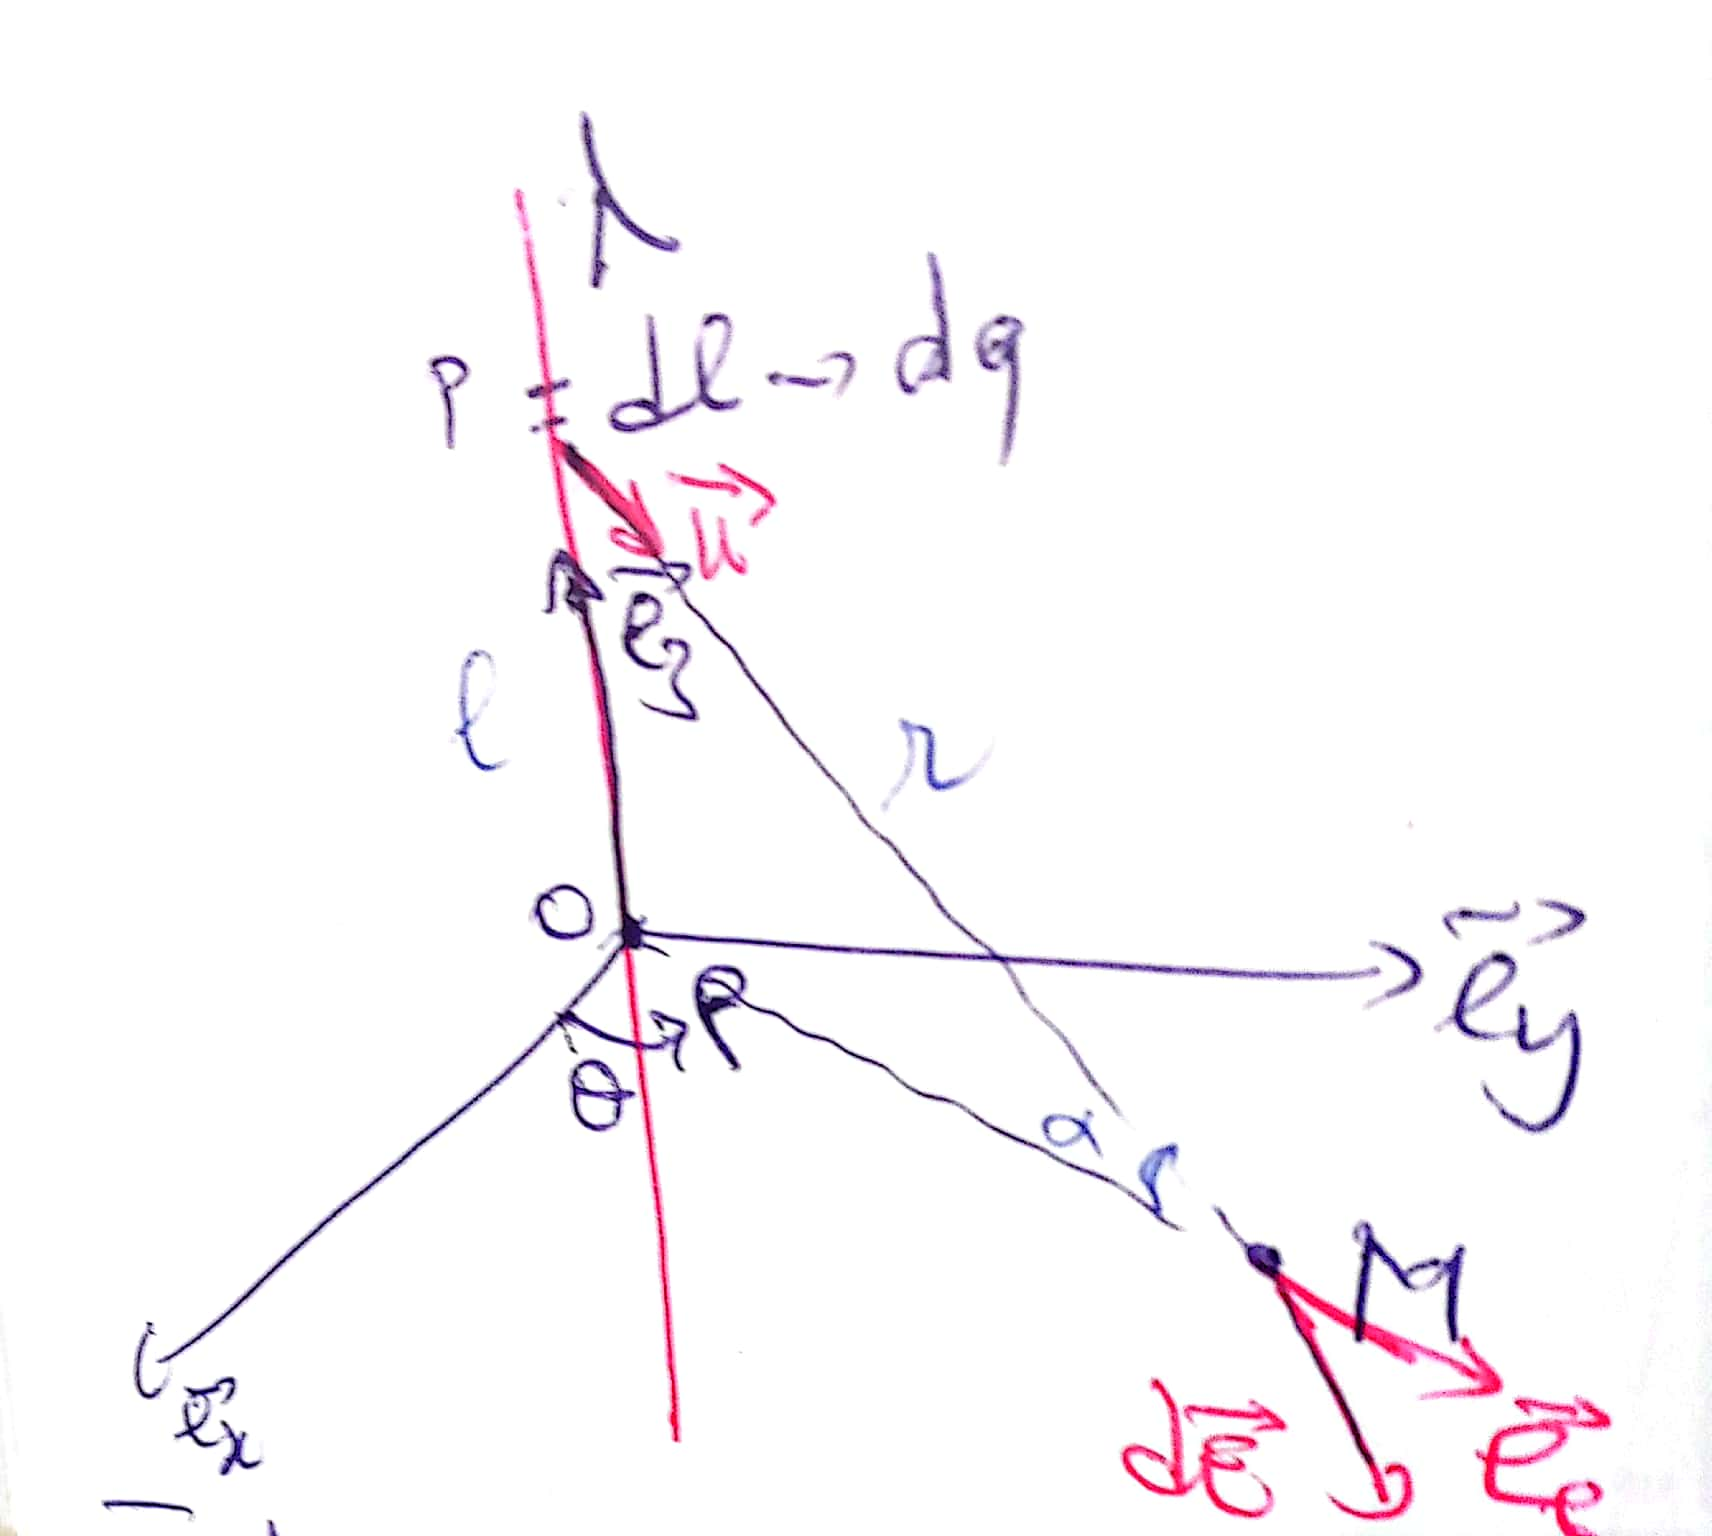
\includegraphics[width=0.7\textwidth]{images/electrostatique/elecst-007-001.png}
\captionof{figure}{\small Sphère chargée uniformément en volume : surface de Gauss sphérique et lignes de champ radial.}
\end{center}
\end{boitecorrige}

\subsection*{Exercice 3 - Condensateur plan \niveau{\facile}}

\begin{boiteexercice}
Un condensateur plan est constitué de deux armatures parallèles de surface $S = \qty{100}{cm^2}$, séparées d'une distance $d = \qty{2}{mm}$ dans le vide.
\begin{enumerate}
  \item Calculer sa capacité $C$.
  \item Il est chargé sous une tension $U = \qty{100}{V}$. Calculer la charge $Q$, le champ $E$ entre les armatures, et l'énergie stockée $W$.
  \item On insère un diélectrique de permittivité relative $\varepsilon_r = 4$ entre les armatures (à tension constante). Donner les nouvelles valeurs de $C$, $Q$ et $W$.
\end{enumerate}
\end{boiteexercice}

\begin{boitecorrige}
\textbf{1.} $C = \varepsilon_0 S/d = 8{,}85\times10^{-12}\times10^{-2}/(2\times10^{-3}) = \qty{44.25}{pF}$.

\textbf{2.} $Q = CU = 44{,}25\times10^{-12}\times100 = \qty{4.425}{nC}$.
$E = U/d = 100/(2\times10^{-3}) = \qty{50000}{V.m^{-1}}$.
$W = \frac{1}{2}CU^2 = \frac{1}{2}\times44{,}25\times10^{-12}\times10^4 = \qty{221}{pJ}$.

\textbf{3.} Avec le diélectrique (tension constante $U = \qty{100}{V}$) :
$C' = \varepsilon_r C = 4\times44{,}25 = \qty{177}{pF}$.
$Q' = C'U = \qty{17.7}{nC}$.
$W' = \frac{1}{2}C'U^2 = 4W = \qty{884}{pJ}$.

L'énergie augmente car le générateur a fourni de l'énergie supplémentaire pour maintenir la tension constante pendant l'insertion.

\begin{center}

\includegraphics[width=0.7\textwidth]{images/electrostatique/elecst-009-002.png}
\captionof{figure}{\small Condensateur plan : armatures métalliques parallèles et champ $\vec{E}$ uniforme entre les plaques.}
\end{center}
\end{boitecorrige}

\subsection*{Exercice 4 - Théorème d'Ampère : solénoïde et fil infini \niveau{\moyen}}

\begin{boiteexercice}
\begin{enumerate}
  \item Un fil rectiligne infini parcouru par un courant $I = \qty{10}{A}$. Calculer le champ magnétique $B$ à la distance $r = \qty{5}{cm}$ du fil.
  \item Un solénoïde de longueur $L = \qty{20}{cm}$, comportant $N = 500$ spires, parcouru par $I = \qty{2}{A}$. Calculer le champ $B$ à l'intérieur.
  \item Calculer le flux magnétique à travers une spire de rayon $a = \qty{1}{cm}$ du solénoïde.
\end{enumerate}
\textbf{Donnée :} $\mu_0 = 4\pi\times10^{-7}\,\text{H.m}^{-1}$.
\end{boiteexercice}

\begin{boitecorrige}
\textbf{1.} Pour un fil infini, par symétrie cylindrique, le théorème d'Ampère sur un cercle de rayon $r$ donne $B\times 2\pi r = \mu_0 I$, d'où :
\[
B = \frac{\mu_0 I}{2\pi r} = \frac{4\pi\times10^{-7}\times10}{2\pi\times0{,}05} = \qty{40}{\mu T}
\]

\begin{center}
\begin{tikzpicture}[scale=1.0]
  % Fil rectiligne infini (axe z)
  \draw[very thick, gray!70] (0,-2.5) -- (0,2.5);
  \draw[->, very thick, gray!80] (0,0) -- (0,1.8) node[right, font=\small] {$I\,\hat{z}$};
  % Contour d'Ampère circulaire
  \draw[blue!70, thick, dashed] (0,0) ellipse (1.5 and 0.45);
  \draw[->, blue!70, thick] (1.5,0) arc (0:30:1.5 and 0.45);
  \node[blue!80, font=\small] at (2.2, 0) {contour d'Ampère};
  % Rayon r
  \draw[<->, red!70] (0,0) -- (1.5,0) node[midway, above, font=\small] {$r$};
  % Vecteur B tangentiel
  \draw[->, red!80, thick] (1.5, 0.3) arc (90:150:0.5);
  \node[red!80, font=\small] at (2.0, 0.55) {$\vec{B}$};
\end{tikzpicture}
\captionof{figure}{\small Symétrie cylindrique : le fil infini (gris) est le centre du contour d'Ampère circulaire (bleu) de rayon $r$. Le champ $\vec{B}$ est orthoradial.}
\end{center}

\textbf{2.} À l'intérieur d'un solénoïde de densité linéique de spires $n = N/L = 500/0{,}2 = 2500\,\text{spires.m}^{-1}$ :
\[
B = \mu_0 n I = 4\pi\times10^{-7}\times2500\times2 \approx \qty{6.28}{mT}
\]

\textbf{3.} Le flux à travers une spire de section $\pi a^2$ :
\[
\Phi = B\times\pi a^2 = 6{,}28\times10^{-3}\times\pi\times(10^{-2})^2 \approx \qty{1.97e-6}{Wb}
\]
\end{boitecorrige}


\subsection*{Exercice 5 - Distribution linéique : anneau chargé \niveau{\moyen}}

\begin{boiteexercice}
Un anneau de rayon $R = \qty{5}{cm}$ porte une charge totale $Q = \qty{2e-9}{C}$ uniformément répartie.
\begin{enumerate}
  \item Calculer le champ électrique $E$ au centre de l'anneau.
  \item Exprimer le champ électrique $E(z)$ sur l'axe de l'anneau à une distance $z$ du centre.
  \item Calculer $E(z)$ pour $z = \qty{3}{cm}$.
  \item Pour quelle valeur de $z$ le champ est-il maximal sur l'axe ?
\end{enumerate}
\textbf{Donnée :} $k = 1/(4\pi\varepsilon_0) = \qty{9e9}{N.m^2.C^{-2}}$.
\end{boiteexercice}

\begin{boitecorrige}
\textbf{1.} Par symétrie, les composantes radiales du champ se compensent en tout point de l'anneau. Au centre ($z=0$), toutes les contributions se compensent par symétrie azimutale : $\boxed{E_{centre} = 0}$.

\textbf{2.} Champ sur l'axe : chaque élément de charge $\d q$ crée un champ élémentaire. Par symétrie de révolution, seule la composante axiale $\d E_z$ survit. Pour un élément $\d q$ à distance $r = \sqrt{R^2+z^2}$ du point $P$ sur l'axe :
\[
\d E_z = \frac{k\,\d q}{R^2+z^2}\cdot\frac{z}{\sqrt{R^2+z^2}} = \frac{k\,\d q\,z}{(R^2+z^2)^{3/2}}
\]
En intégrant sur tout l'anneau :
\[
\boxed{E(z) = \frac{kQz}{(R^2+z^2)^{3/2}}}
\]

\textbf{3.} Pour $z = \qty{0.03}{m}$, $R = \qty{0.05}{m}$ :
\begin{align}
E &= \frac{9\times10^9 \times 2\times10^{-9} \times 0{,}03}{((0{,}05)^2+(0{,}03)^2)^{3/2}} \notag \\
&= \frac{0{,}54}{(0{,}0025+0{,}0009)^{3/2}} = \frac{0{,}54}{(0{,}0034)^{3/2}}
\end{align}
$(0{,}0034)^{3/2} = (0{,}0034)^1 \times (0{,}0034)^{1/2} = 0{,}0034 \times 0{,}05831 \approx 1{,}982\times10^{-4}$
\[
E \approx \frac{0{,}54}{1{,}982\times10^{-4}} \approx \qty{2724}{V.m^{-1}}
\]

\textbf{4.} On maximise $E(z)$ en dérivant et en annulant :
\[
\frac{\d E}{\d z} = kQ\frac{(R^2+z^2)^{3/2} - z\cdot\frac{3}{2}(R^2+z^2)^{1/2}\cdot2z}{(R^2+z^2)^3} = 0
\]
Le numérateur s'annule quand $(R^2+z^2) - 3z^2 = 0$, soit $R^2 = 2z^2$, donc :
\[
z_{max} = \frac{R}{\sqrt{2}} = \frac{0{,}05}{\sqrt{2}} \approx \qty{3.54}{cm}
\]

\begin{center}
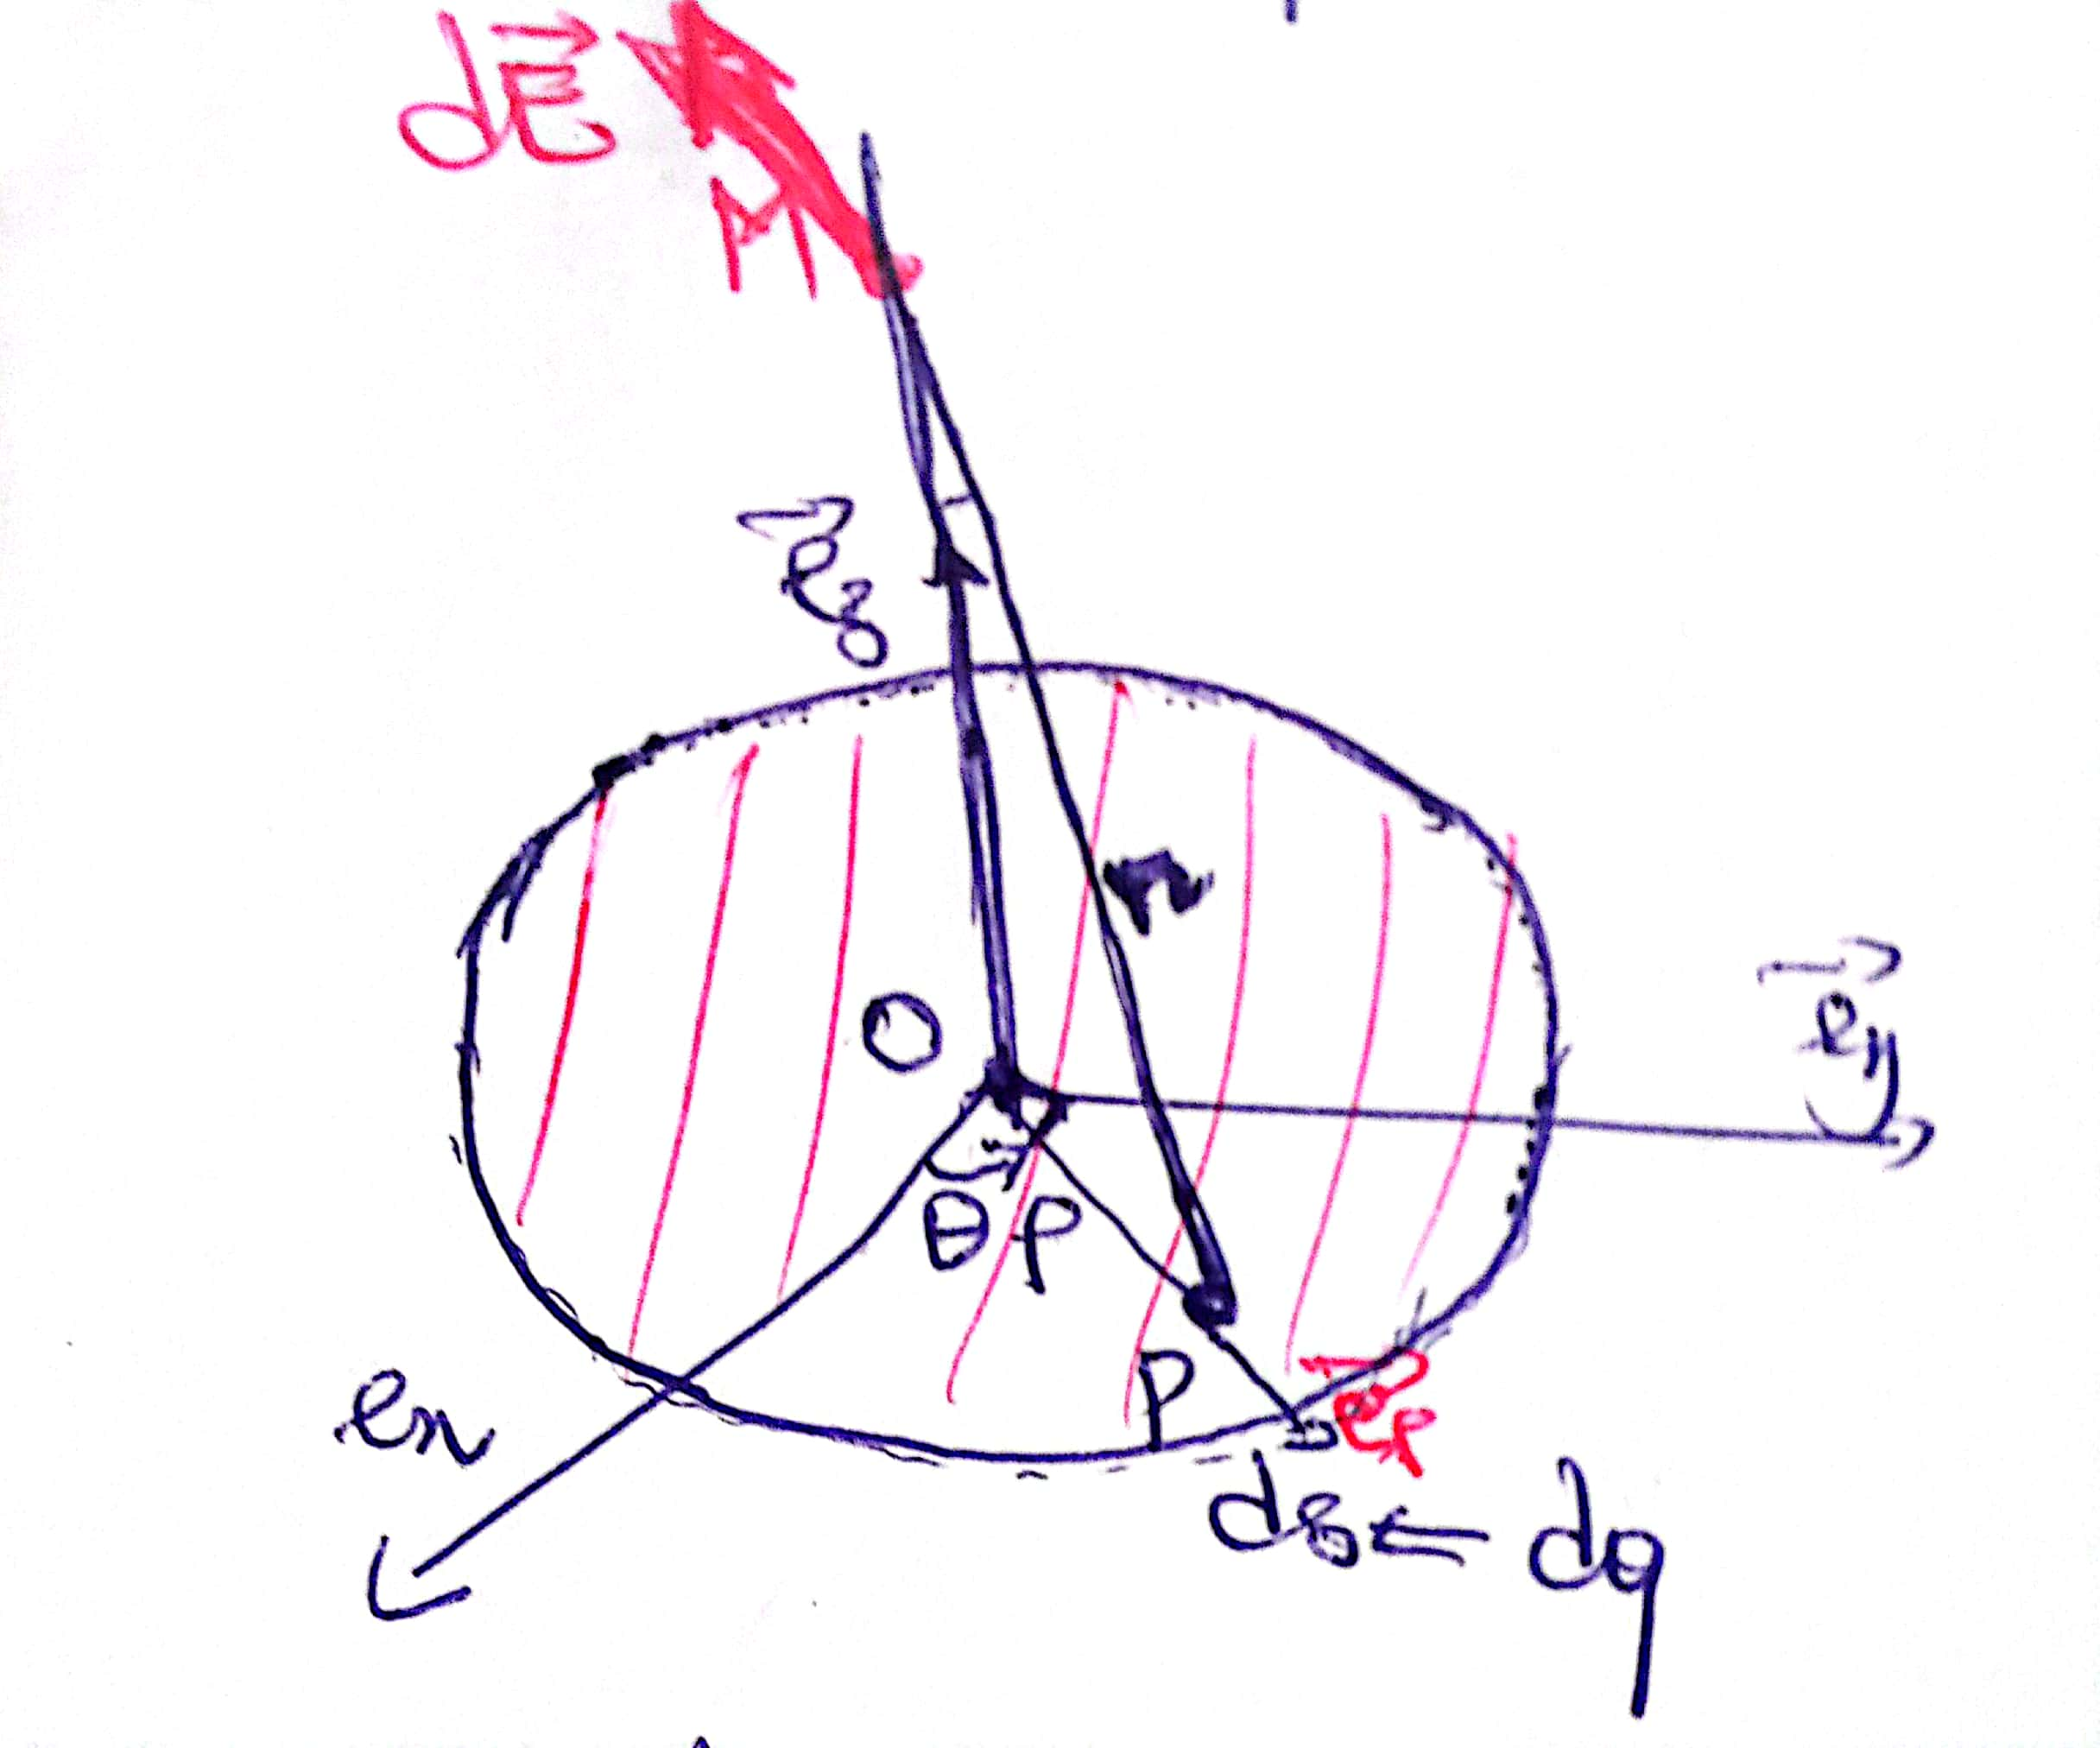
\includegraphics[width=0.7\textwidth]{images/electrostatique/elecst-009-003.png}
\captionof{figure}{\small Anneau chargé : élément $\d q$ et champ élémentaire $\d\vec{E}$ sur l'axe de révolution.}
\end{center}
\end{boitecorrige}

\subsection*{Exercice 6 - Condensateur plan chargé \niveau{\facile}}

\newpage
\begin{boiteexercice}
Un condensateur plan est formé de deux plaques parallèles de surface $S = \qty{200}{cm^2}$, distantes de $d = \qty{2}{mm}$, soumises à une tension $V = \qty{500}{V}$.
\begin{enumerate}
  \item Calculer le champ électrique $E$ entre les armatures.
  \item Calculer la capacité $C = \varepsilon_0 S/d$.
  \item Calculer la charge $Q$ sur les armatures.
  \item Calculer l'énergie stockée $U = \frac{1}{2}CV^2$.
\end{enumerate}
\textbf{Donnée :} $\varepsilon_0 = \qty{8.85e-12}{F.m^{-1}}$.
\end{boiteexercice}

\begin{boitecorrige}
\textbf{1.} Champ uniforme entre les plaques :
\[
E = \frac{V}{d} = \frac{500}{2\times10^{-3}} = \qty{2.5e5}{V.m^{-1}}
\]

\textbf{2.} Capacité :
\[
C = \frac{\varepsilon_0 S}{d} = \frac{8{,}85\times10^{-12}\times200\times10^{-4}}{2\times10^{-3}}
= 88{,}5\times10^{-12}\,\text{F} \approx \qty{88.5}{pF}
\]

\textbf{3.} Charge sur les armatures :
\[
Q = CV = 88{,}5\times10^{-12}\times500 = \qty{44.25}{nC}
\]

\textbf{4.} Énergie stockée :
\[
U = \frac{1}{2}CV^2 = \frac{1}{2}\times88{,}5\times10^{-12}\times(500)^2 = \frac{1}{2}\times88{,}5\times10^{-12}\times2{,}5\times10^5 \approx \qty{11.1}{\mu J}
\]
\end{boitecorrige}

\subsection*{Exercice 7 - Théorème de Gauss : sphère uniformément chargée \niveau{\moyen}}

\begin{boiteexercice}
Une sphère isolante de rayon $R = \qty{10}{cm}$ porte une charge totale $Q = \qty{1e-8}{C}$ répartie uniformément en volume (densité volumique $\rho = Q/(\frac{4}{3}\pi R^3)$).
\begin{enumerate}
  \item Appliquer le théorème de Gauss pour calculer $\vec{E}$ à l'intérieur ($r < R$).
  \item Calculer $\vec{E}$ à l'extérieur ($r > R$).
  \item Calculer $E$ à $r = \qty{5}{cm}$ et à $r = \qty{20}{cm}$.
\end{enumerate}
\end{boiteexercice}

\begin{boitecorrige}
Par symétrie sphérique, $\vec{E} = E(r)\,\hat{r}$.

\textbf{1. À l'intérieur ($r < R$) :} La charge enfermée dans une sphère de rayon $r$ est :
\[
Q_{int} = \rho \cdot \frac{4}{3}\pi r^3 = Q\cdot\frac{r^3}{R^3}
\]
Le théorème de Gauss donne $E(r)\cdot 4\pi r^2 = Q_{int}/\varepsilon_0$ :
\[
\boxed{E(r<R) = \frac{Qr}{4\pi\varepsilon_0 R^3}}
\]
Le champ croît linéairement avec $r$ à l'intérieur.

\textbf{2. À l'extérieur ($r > R$) :} Toute la charge $Q$ est enfermée :
\[
E(r>R)\cdot 4\pi r^2 = \frac{Q}{\varepsilon_0} \quad \Rightarrow \quad \boxed{E(r>R) = \frac{Q}{4\pi\varepsilon_0 r^2}}
\]
La sphère se comporte comme une charge ponctuelle.

\textbf{3.} Pour $r = \qty{0.05}{m}$ (intérieur) :
\[
E = \frac{9\times10^9\times10^{-8}\times0{,}05}{(0{,}10)^3} = \frac{4{,}5\times10^0}{10^{-3}} = \qty{4500}{V.m^{-1}}
\]
Pour $r = \qty{0.20}{m}$ (extérieur) :
\[
E = \frac{9\times10^9\times10^{-8}}{(0{,}20)^2} = \frac{90}{0{,}04} = \qty{2250}{V.m^{-1}}
\]
\end{boitecorrige}

\subsection*{Exercice 8 - Plan infini chargé \niveau{\moyen}}

\begin{boiteexercice}
Un plan infini porte une densité surfacique de charges $\sigma = \qty{2e-6}{C.m^{-2}}$.
\begin{enumerate}
  \item Calculer le champ électrique $E$ de part et d'autre du plan en utilisant le théorème de Gauss.
  \item Que vaut la discontinuité du champ électrique normal à la traversée du plan ?
  \item Calculer numériquement $E$.
\end{enumerate}
\end{boiteexercice}

\begin{boitecorrige}
\textbf{1.} On choisit comme surface de Gauss un cylindre de section $S$ traversant le plan, dont les deux bases sont parallèles au plan chargé. Par symétrie, le champ est perpendiculaire au plan et de même module des deux côtés.

\begin{center}
\begin{tikzpicture}[scale=0.9]
  % Plan infini chargé (en gris)
  \fill[gray!20] (-3.5,-0.12) rectangle (3.5,0.12);
  \draw[gray!60, thick] (-3.5, 0) -- (3.5, 0);
  \node[gray!80, font=\small] at (3.8, 0) {$\sigma$};
  % Cylindre de Gauss
  \draw[blue!60, thick] (-1.0,-0.12) rectangle (1.0, 0.12); % section visible
  \draw[blue!60, thick] (-1.0, 1.2) -- (-1.0,-1.2);
  \draw[blue!60, thick] (1.0, 1.2) -- (1.0,-1.2);
  \draw[blue!60, thick, dashed] (0, 1.2) ellipse (1.0 and 0.25);
  \draw[blue!60, thick] (0, -1.2) ellipse (1.0 and 0.25);
  \node[blue!70, font=\scriptsize] at (1.7, 0.8) {Surface de Gauss};
  % Flèches champ E
  \draw[->, red!70, very thick] (0, 0.12) -- (0, 1.0) node[right, font=\small] {$\vec{E}$};
  \draw[->, red!70, very thick] (0, -0.12) -- (0, -1.0) node[right, font=\small] {$\vec{E}$};
  % Section S
  \draw[<->, darkgray] (-1.0, 1.45) -- (1.0, 1.45) node[midway, above, font=\scriptsize] {$\sqrt{S}$};
\end{tikzpicture}
\captionof{figure}{\small Surface de Gauss (cylindre bleu) traversant le plan chargé $\sigma$. Le flux traverse uniquement les deux bases (surfaces parallèles au plan).}
\end{center}

Le flux total est $\Phi = 2ES$ (deux bases) et la charge enfermée est $Q_{int} = \sigma S$.

Le théorème de Gauss donne :
\[
2ES = \frac{\sigma S}{\varepsilon_0} \quad \Rightarrow \quad \boxed{E = \frac{\sigma}{2\varepsilon_0}}
\]
Le champ est dirigé vers l'extérieur du plan des deux côtés.

\textbf{2.} La discontinuité du champ normal à la traversée d'une surface chargée (surface avec $\sigma$) est :
\[
\Delta E_n = E_{au\text{-}dessus} - E_{en\text{-}dessous} = \frac{\sigma}{\varepsilon_0}
\]
Ici, $E_{au\text{-}dessus} = +\sigma/(2\varepsilon_0)$ et $E_{en\text{-}dessous} = -\sigma/(2\varepsilon_0)$, donc la saut vaut bien $\sigma/\varepsilon_0$.

\textbf{3.} Calcul numérique :
\[
E = \frac{\sigma}{2\varepsilon_0} = \frac{2\times10^{-6}}{2\times8{,}85\times10^{-12}} = \frac{2\times10^{-6}}{1{,}77\times10^{-11}} \approx \qty{1.13e5}{V.m^{-1}}
\]
\end{boitecorrige}

\subsection*{Exercice 9 - Conducteur sphérique creux \niveau{\moyen}}

\begin{boiteexercice}
Un conducteur sphérique creux a un rayon interne $R_1 = \qty{5}{cm}$ et un rayon externe $R_2 = \qty{8}{cm}$. Il porte une charge totale $Q = \qty{3e-9}{C}$.
\begin{enumerate}
  \item Décrire la distribution des charges sur le conducteur.
  \item Calculer le champ électrique dans les trois zones : $r < R_1$, $R_1 < r < R_2$ (métal), et $r > R_2$.
  \item Si l'on place une charge $q = \qty{1e-9}{C}$ à l'intérieur de la cavité, décrire à nouveau la distribution des charges.
\end{enumerate}
\end{boiteexercice}

\begin{boitecorrige}
\textbf{1. Distribution des charges (sans charge intérieure) :} Dans un conducteur à l'équilibre, le champ intérieur est nul. Toute la charge $Q$ se place sur la \textbf{surface externe} ($r = R_2$). Il n'y a aucune charge sur la surface interne ($r = R_1$) car la cavité est vide.

\textbf{2. Champ électrique :}
\begin{itemize}
  \item Zone $r < R_1$ (intérieur de la cavité) : $\vec{E} = \vec{0}$ (aucune charge enfermée).
  \item Zone $R_1 < r < R_2$ (métal) : $\vec{E} = \vec{0}$ (propriété du conducteur à l'équilibre).
  \item Zone $r > R_2$ : par Gauss, $E = \dfrac{Q}{4\pi\varepsilon_0 r^2}$.
\end{itemize}

\textbf{3. Avec charge $q$ dans la cavité :} Par le théorème de Gauss (surface dans le métal où $E=0$), la charge enfermée est nulle, donc il apparaît $-q$ sur la surface interne ($r=R_1$). La charge totale sur le conducteur étant $Q$, la surface externe porte $Q+q = \qty{3e-9}{C} + \qty{1e-9}{C} = \qty{4e-9}{C}$.

À l'extérieur ($r > R_2$) : $E = \dfrac{Q+q}{4\pi\varepsilon_0 r^2}$.

\begin{center}

\includegraphics[width=0.7\textwidth]{images/electrostatique/elecst-013-006.png}
\captionof{figure}{\small Conducteur sphérique creux : distribution des charges sur les surfaces internes et externes.}
\end{center}
\end{boitecorrige}

\newpage
\section{Magnétostatique}

\subsection*{Exercice 10 - Champ d'un fil infini \niveau{\facile}}

\begin{boiteexercice}
Un fil rectiligne infini est parcouru par un courant $I = \qty{10}{A}$.
\begin{enumerate}
  \item En appliquant la loi de Biot-Savart (ou le théorème d'Ampère), montrer que le champ magnétique à la distance $r$ du fil est $B = \dfrac{\mu_0 I}{2\pi r}$.
  \item Calculer $B$ à $r = \qty{5}{cm}$ du fil.
  \item Calculer $B$ à $r = \qty{1}{cm}$ et $r = \qty{20}{cm}$.
\end{enumerate}
\textbf{Donnée :} $\mu_0 = 4\pi\times10^{-7}\,\text{H.m}^{-1}$.
\end{boiteexercice}

\begin{boitecorrige}
\textbf{1.} Par symétrie cylindrique, le champ $\vec{B}$ est orthoradial ($\vec{B} = B(r)\,\hat{\phi}$). On applique le théorème d'Ampère sur un cercle de rayon $r$ centré sur le fil :
\[
\oint \vec{B}\cdot\d\vec{l} = B\cdot 2\pi r = \mu_0 I_{\text{enlacé}} = \mu_0 I
\]
\[
\boxed{B = \frac{\mu_0 I}{2\pi r}}
\]

\begin{center}
\begin{tikzpicture}[scale=1.0]
  % Fil (point central avec courant sortant)
  \draw[fill=gray!40] (0,0) circle (0.18);
  \draw[thick] (-0.13,-0.13) -- (0.13,0.13);
  \draw[thick] (-0.13,0.13) -- (0.13,-0.13);
  \node[font=\small] at (0.55, 0) {$I\,(\odot)$};
  % Lignes de champ B circulaires
  \foreach \r in {0.7, 1.3, 2.0} {
    \draw[red!60, thick] (0,0) circle (\r);
    \draw[->, red!70, thick] (\r, 0) arc(0:20:\r);
  }
  % Étiquette B
  \node[red!70, font=\small] at (2.3, 0.6) {$\vec{B}$};
  % Rayon r
  \draw[<->, blue!70] (0,0) -- (1.3,0) node[midway, above, font=\small] {$r$};
  % Graphe B(r) sur le côté
  \begin{scope}[xshift=4.5cm, yshift=-1cm]
    \draw[->] (0,0) -- (3.2,0) node[right, font=\scriptsize] {$r$};
    \draw[->] (0,0) -- (0,2.5) node[above, font=\scriptsize] {$B(r)$};
    \draw[red!70, very thick, domain=0.3:3.0, samples=50]
      plot(\x, {1.2/\x});
    \node[font=\scriptsize, red!70] at (2.0, 0.9) {$B\propto 1/r$};
  \end{scope}
\end{tikzpicture}
\captionof{figure}{\small Gauche : lignes de champ $\vec{B}$ circulaires autour d'un fil infini (vue en coupe). Droite : graphe de $B(r)$ montrant la décroissance en $1/r$.}
\end{center}

\textbf{2.} À $r = \qty{0.05}{m}$ :
\[
B = \frac{4\pi\times10^{-7}\times10}{2\pi\times0{,}05} = \frac{4\times10^{-6}}{0{,}1} = \qty{40}{\mu T}
\]

\textbf{3.}
\[
B(1\,\text{cm}) = \frac{4\pi\times10^{-7}\times10}{2\pi\times0{,}01} = \qty{200}{\mu T}
\]
\[
B(20\,\text{cm}) = \frac{4\pi\times10^{-7}\times10}{2\pi\times0{,}20} = \qty{10}{\mu T}
\]
Le champ décroît en $1/r$ : en doublant la distance, $B$ est divisé par 2.
\end{boitecorrige}

\subsection*{Exercice 11 - Champ d'un solénoïde \niveau{\facile}}

\begin{boiteexercice}
Un solénoïde infini comporte $n = \qty{1000}{spires.m^{-1}}$ et est parcouru par un courant $I = \qty{2}{A}$.
\begin{enumerate}
  \item Calculer le champ magnétique $B$ à l'intérieur du solénoïde.
  \item Quel est le champ à l'extérieur du solénoïde (pour un solénoïde infini idéal) ?
  \item Calculer le flux magnétique à travers une section circulaire de rayon $a = \qty{2}{cm}$.
\end{enumerate}
\textbf{Donnée :} $\mu_0 = 4\pi\times10^{-7}\,\text{H.m}^{-1}$.
\end{boiteexercice}

\begin{boitecorrige}
\textbf{1.} On applique le théorème d'Ampère sur un rectangle de longueur $l$ dont un côté est à l'intérieur (où $B$ est uniforme et axial) et l'autre à l'extérieur (où $B\approx0$). Le courant enlacé est $I_{\text{enlacé}} = n\,l\,I$.
\[
B\cdot l = \mu_0\,n\,l\,I \quad \Rightarrow \quad \boxed{B = \mu_0 n I}
\]
\[
B = 4\pi\times10^{-7}\times1000\times2 = 4\pi\times10^{-4} \approx \qty{2.51}{mT}
\]

\textbf{2.} À l'extérieur d'un solénoïde infini idéal, le champ est nul : $B_{ext} = 0$. (En pratique, pour un solénoïde fini, il subsiste un champ résiduel faible à l'extérieur.)

\textbf{3.} Flux à travers la section $\pi a^2$ :
\[
\Phi = B\cdot\pi a^2 = 2{,}51\times10^{-3}\times\pi\times(0{,}02)^2 = 2{,}51\times10^{-3}\times1{,}257\times10^{-3} \approx \qty{3.15}{\mu Wb}
\]
\end{boitecorrige}

\subsection*{Exercice 12 - Théorème d'Ampère : tore \niveau{\difficile}}

\begin{boiteexercice}
Un tore de rayon moyen $r_0 = \qty{10}{cm}$, de section circulaire de rayon $a = \qty{1}{cm}$, comporte $N = 500$ spires portant un courant $I = \qty{3}{A}$.
\begin{enumerate}
  \item En appliquant le théorème d'Ampère $\oint \vec{B}\cdot\d\vec{l} = \mu_0 I_{\text{enlacé}}$, calculer le champ $B$ à l'intérieur du tore (à $r = r_0$).
  \item Quel est le champ à l'extérieur du tore ?
  \item Calculer l'inductance propre $L = N\Phi/I$ du tore, avec $\Phi = B\cdot\pi a^2$.
\end{enumerate}
\textbf{Donnée :} $\mu_0 = 4\pi\times10^{-7}\,\text{H.m}^{-1}$.
\end{boiteexercice}

\begin{boitecorrige}
\textbf{1.} On choisit un contour d'Ampère circulaire de rayon $r = r_0$ à l'intérieur du tore. Par symétrie de révolution, $\vec{B}$ est tangentiel et uniforme sur ce contour. Le courant enlacé est $I_{\text{enlacé}} = N\cdot I$ (toutes les spires traversent la surface délimitée par le contour) :
\[
B\cdot 2\pi r_0 = \mu_0 N I
\]
\[
B = \frac{\mu_0 N I}{2\pi r_0} = \frac{4\pi\times10^{-7}\times500\times3}{2\pi\times0{,}10} = \frac{6\pi\times10^{-4}}{\pi\times0{,}2} = \frac{6\times10^{-4}}{0{,}2} = \qty{3}{mT}
\]

\textbf{2.} Pour un contour extérieur au tore, le courant enlacé est nul (les courants aller et retour se compensent pour chaque spire) : $B_{ext} = 0$.

\textbf{3.} Inductance propre :
\[
\Phi = B\cdot\pi a^2 = 3\times10^{-3}\times\pi\times(10^{-2})^2 = 3\times10^{-3}\times\pi\times10^{-4} \approx \qty{9.42e-7}{Wb}
\]
\[
L = \frac{N\Phi}{I} = \frac{500\times9{,}42\times10^{-7}}{3} = \frac{4{,}71\times10^{-4}}{3} \approx \qty{157}{\mu H}
\]
\end{boitecorrige}


\subsection*{Exercice 13 - Anneau chargé : champ sur l'axe \niveau{\moyen}}

\begin{boiteexercice}
Un anneau de rayon $R = \qty{10}{cm}$ porte une charge totale $Q = \qty{2e-6}{C}$ répartie uniformément.
\begin{enumerate}
  \item Calculer le champ électrique en $z = 0$ (centre de l'anneau).
  \item Rappeler la formule du champ sur l'axe :
  \[
  E(z) = \frac{Qz}{4\pi\varepsilon_0(R^2+z^2)^{3/2}}
  \]
  \item Calculer numériquement $E$ en $z = R/\sqrt{2}$.
  \item Pour quelle valeur de $z$ le champ est-il maximum sur l'axe ?
\end{enumerate}
\textbf{Donnée :} $k = 1/(4\pi\varepsilon_0) = \qty{9e9}{N.m^2.C^{-2}}$.
\end{boiteexercice}

\begin{boitecorrige}
\textbf{1.} En $z = 0$, par symétrie azimutale, toutes les contributions radiales se compensent et la composante axiale de chaque élément $\d E_z = k\,\d q\cdot 0/(R^2)^{3/2} = 0$. Donc : $\boxed{E(0) = 0}$.

\textbf{2.} Chaque élément de charge $\d q$ crée sur l'axe une contribution dont seule la composante axiale $\d E_z = k\,\d q\,z/(R^2+z^2)^{3/2}$ survit par symétrie. En intégrant :
\[
E(z) = \frac{kQz}{(R^2+z^2)^{3/2}}
\]

\textbf{3.} En $z = R/\sqrt{2}$ avec $R = 0{,}1\,\text{m}$ :
\[
R^2 + z^2 = R^2 + \frac{R^2}{2} = \frac{3R^2}{2} = \frac{3\times0{,}01}{2} = 0{,}015\,\text{m}^2
\]
\[
(R^2+z^2)^{3/2} = (0{,}015)^{3/2} = 0{,}015\times\sqrt{0{,}015} = 0{,}015\times0{,}1225 \approx 1{,}837\times10^{-3}
\]
\[
E = \frac{9\times10^9\times2\times10^{-6}\times0{,}07071}{1{,}837\times10^{-3}} \approx \qty{6.93e6}{V.m^{-1}}
\]

\textbf{4.} Le maximum de $E(z)$ s'obtient en annulant $\d E/\d z = 0$. On trouve $z_{max} = R/\sqrt{2}$, soit :
\[
z_{max} = \frac{0{,}1}{\sqrt{2}} \approx \qty{7.07}{cm}
\]
\end{boitecorrige}

\subsection*{Exercice 14 - Condensateur plan : calcul complet \niveau{\facile}}

\begin{boiteexercice}
Un condensateur plan a des armatures de surface $S = \qty{0.01}{m^2}$, séparées de $d = \qty{2}{mm}$, soumises à une tension $V = \qty{500}{V}$.
\begin{enumerate}
  \item Calculer le champ électrique $E = V/d$ entre les armatures.
  \item Calculer la capacité $C = \varepsilon_0 S/d$ (dans le vide).
  \item Calculer l'énergie stockée $U = \frac{1}{2}CV^2$.
  \item Donner la densité d'énergie électrostatique $u = \frac{1}{2}\varepsilon_0 E^2$.
\end{enumerate}
\textbf{Donnée :} $\varepsilon_0 = \qty{8.85e-12}{F.m^{-1}}$.
\end{boiteexercice}

\begin{boitecorrige}
\textbf{1.} Champ uniforme entre les armatures :
\[
E = \frac{V}{d} = \frac{500}{2\times10^{-3}} = \qty{2.5e5}{V.m^{-1}}
\]

\textbf{2.} Capacité :
\[
C = \frac{\varepsilon_0 S}{d} = \frac{8{,}85\times10^{-12}\times0{,}01}{2\times10^{-3}} = \frac{8{,}85\times10^{-14}}{2\times10^{-3}} = \qty{44.25e-12}{F} \approx \qty{44.3}{pF}
\]

\textbf{3.} Énergie stockée :
\[
U = \frac{1}{2}CV^2 = \frac{1}{2}\times44{,}25\times10^{-12}\times(500)^2
\approx \qty{5.53}{\mu J}
\]

\textbf{4.} La densité volumique d'énergie électrostatique vaut :
\[
u = \frac{1}{2}\varepsilon_0 E^2 = \frac{1}{2}\times8{,}85\times10^{-12}\times(2{,}5\times10^5)^2
\approx \qty{0.276}{J.m^{-3}}
\]
Vérification : $U = u\times(S\cdot d) = 0{,}276\times(0{,}01\times2\times10^{-3}) = 0{,}276\times2\times10^{-5} \approx \qty{5.52}{\mu J}$.
\end{boitecorrige}

\subsection*{Exercice 15 - Théorème de Gauss : boule uniformément chargée \niveau{\moyen}}

\begin{boiteexercice}
Une boule isolante de rayon $R = \qty{5}{cm}$ est chargée avec une densité volumique uniforme $\rho = \qty{1e-6}{C.m^{-3}}$.
\begin{enumerate}
  \item Calculer la charge totale $Q = \rho\times\frac{4}{3}\pi R^3$.
  \item En appliquant le théorème de Gauss, exprimer $E(r)$ pour $r < R$ : $E = \rho r/(3\varepsilon_0)$.
  \item Exprimer $E(r)$ pour $r > R$ : $E = \rho R^3/(3\varepsilon_0 r^2)$.
  \item Calculer $E(R)$ par les deux formules et vérifier la continuité.
\end{enumerate}
\textbf{Donnée :} $\varepsilon_0 = \qty{8.85e-12}{F.m^{-1}}$.
\end{boiteexercice}

\begin{boitecorrige}
\textbf{1.} Charge totale :
\[
Q = \rho\times\frac{4}{3}\pi R^3 = 10^{-6}\times\frac{4\pi}{3}\times(0{,}05)^3 = 10^{-6}\times\frac{4\pi}{3}\times1{,}25\times10^{-4} \approx \qty{5.24e-10}{C}
\]

\textbf{2.} Pour $r < R$, la charge intérieure est $Q_{int} = \rho\times\frac{4}{3}\pi r^3$. Le théorème de Gauss sur une sphère de rayon $r$ :
\[
4\pi r^2 E = \frac{Q_{int}}{\varepsilon_0} = \frac{\rho\frac{4}{3}\pi r^3}{\varepsilon_0} \quad \Rightarrow \quad \boxed{E(r<R) = \frac{\rho r}{3\varepsilon_0}}
\]

\textbf{3.} Pour $r > R$, toute la charge est enfermée, $Q_{int} = Q = \rho\frac{4}{3}\pi R^3$ :
\[
4\pi r^2 E = \frac{\rho\frac{4}{3}\pi R^3}{\varepsilon_0} \quad \Rightarrow \quad \boxed{E(r>R) = \frac{\rho R^3}{3\varepsilon_0 r^2}}
\]

\textbf{4.} Calcul de $E(R)$ par les deux formules :
\[
E_{int}(R) = \frac{\rho R}{3\varepsilon_0} = \frac{10^{-6}\times0{,}05}{3\times8{,}85\times10^{-12}} = \frac{5\times10^{-8}}{2{,}655\times10^{-11}} \approx \qty{1884}{V.m^{-1}}
\]
\[
E_{ext}(R) = \frac{\rho R^3}{3\varepsilon_0 R^2} = \frac{\rho R}{3\varepsilon_0} \approx \qty{1884}{V.m^{-1}}
\]
Les deux expressions coïncident en $r = R$ : le champ est continu (pas de discontinuité car il n'y a pas de charge surfacique).

\begin{center}

\includegraphics[width=0.7\textwidth]{images/electrostatique/elecst-012-004.png}
\captionof{figure}{\small Boule uniformément chargée : surface de Gauss sphérique et profil de champ $E(r)$.}
\end{center}
\end{boitecorrige}

\subsection*{Exercice 16 - Plan infini : champ et discontinuité \niveau{\facile}}

\begin{boiteexercice}
Un plan infini porte une densité surfacique de charges $\sigma = \qty{2e-6}{C.m^{-2}}$.
\begin{enumerate}
  \item En utilisant le théorème de Gauss avec un cylindre « pilulier », calculer $E = \sigma/(2\varepsilon_0)$ de chaque côté du plan.
  \item Calculer numériquement $E$.
  \item Exprimer la discontinuité du champ électrique normal à la traversée du plan chargé : $\Delta E_n = \sigma/\varepsilon_0$.
  \item Comparer avec un conducteur plan (surface d'un conducteur) où $E = \sigma/\varepsilon_0$.
\end{enumerate}
\textbf{Donnée :} $\varepsilon_0 = \qty{8.85e-12}{F.m^{-1}}$.
\end{boiteexercice}

\begin{boitecorrige}
\textbf{1.} Surface de Gauss : cylindre de section $S$ traversant le plan, axe perpendiculaire. Les deux bases contribuent au flux ($2ES$), le flux latéral est nul (champ parallèle aux faces latérales) :
\[
2ES = \frac{\sigma S}{\varepsilon_0} \quad \Rightarrow \quad \boxed{E = \frac{\sigma}{2\varepsilon_0}}
\]
Le champ est uniforme, perpendiculaire au plan, dirigé vers l'extérieur des deux côtés.

\textbf{2.} Application numérique :
\[
E = \frac{2\times10^{-6}}{2\times8{,}85\times10^{-12}} = \frac{2\times10^{-6}}{1{,}77\times10^{-11}} \approx \qty{1.13e5}{V.m^{-1}}
\]

\textbf{3.} Le champ est $+\sigma/(2\varepsilon_0)$ d'un côté et $-\sigma/(2\varepsilon_0)$ de l'autre (en convention vectorielle). La discontinuité de la composante normale est :
\[
\Delta E_n = E_{+} - E_{-} = \frac{\sigma}{2\varepsilon_0} - \left(-\frac{\sigma}{2\varepsilon_0}\right) = \frac{\sigma}{\varepsilon_0}
\]

\textbf{4.} Pour la surface d'un conducteur, le champ intérieur est nul. La discontinuité est $E_{ext} - 0 = \sigma/\varepsilon_0$, donc $E_{ext} = \sigma/\varepsilon_0$. C'est le double du champ d'un plan isolant, car pour le conducteur le plan est unilatéral (champ nul d'un côté).

\begin{center}
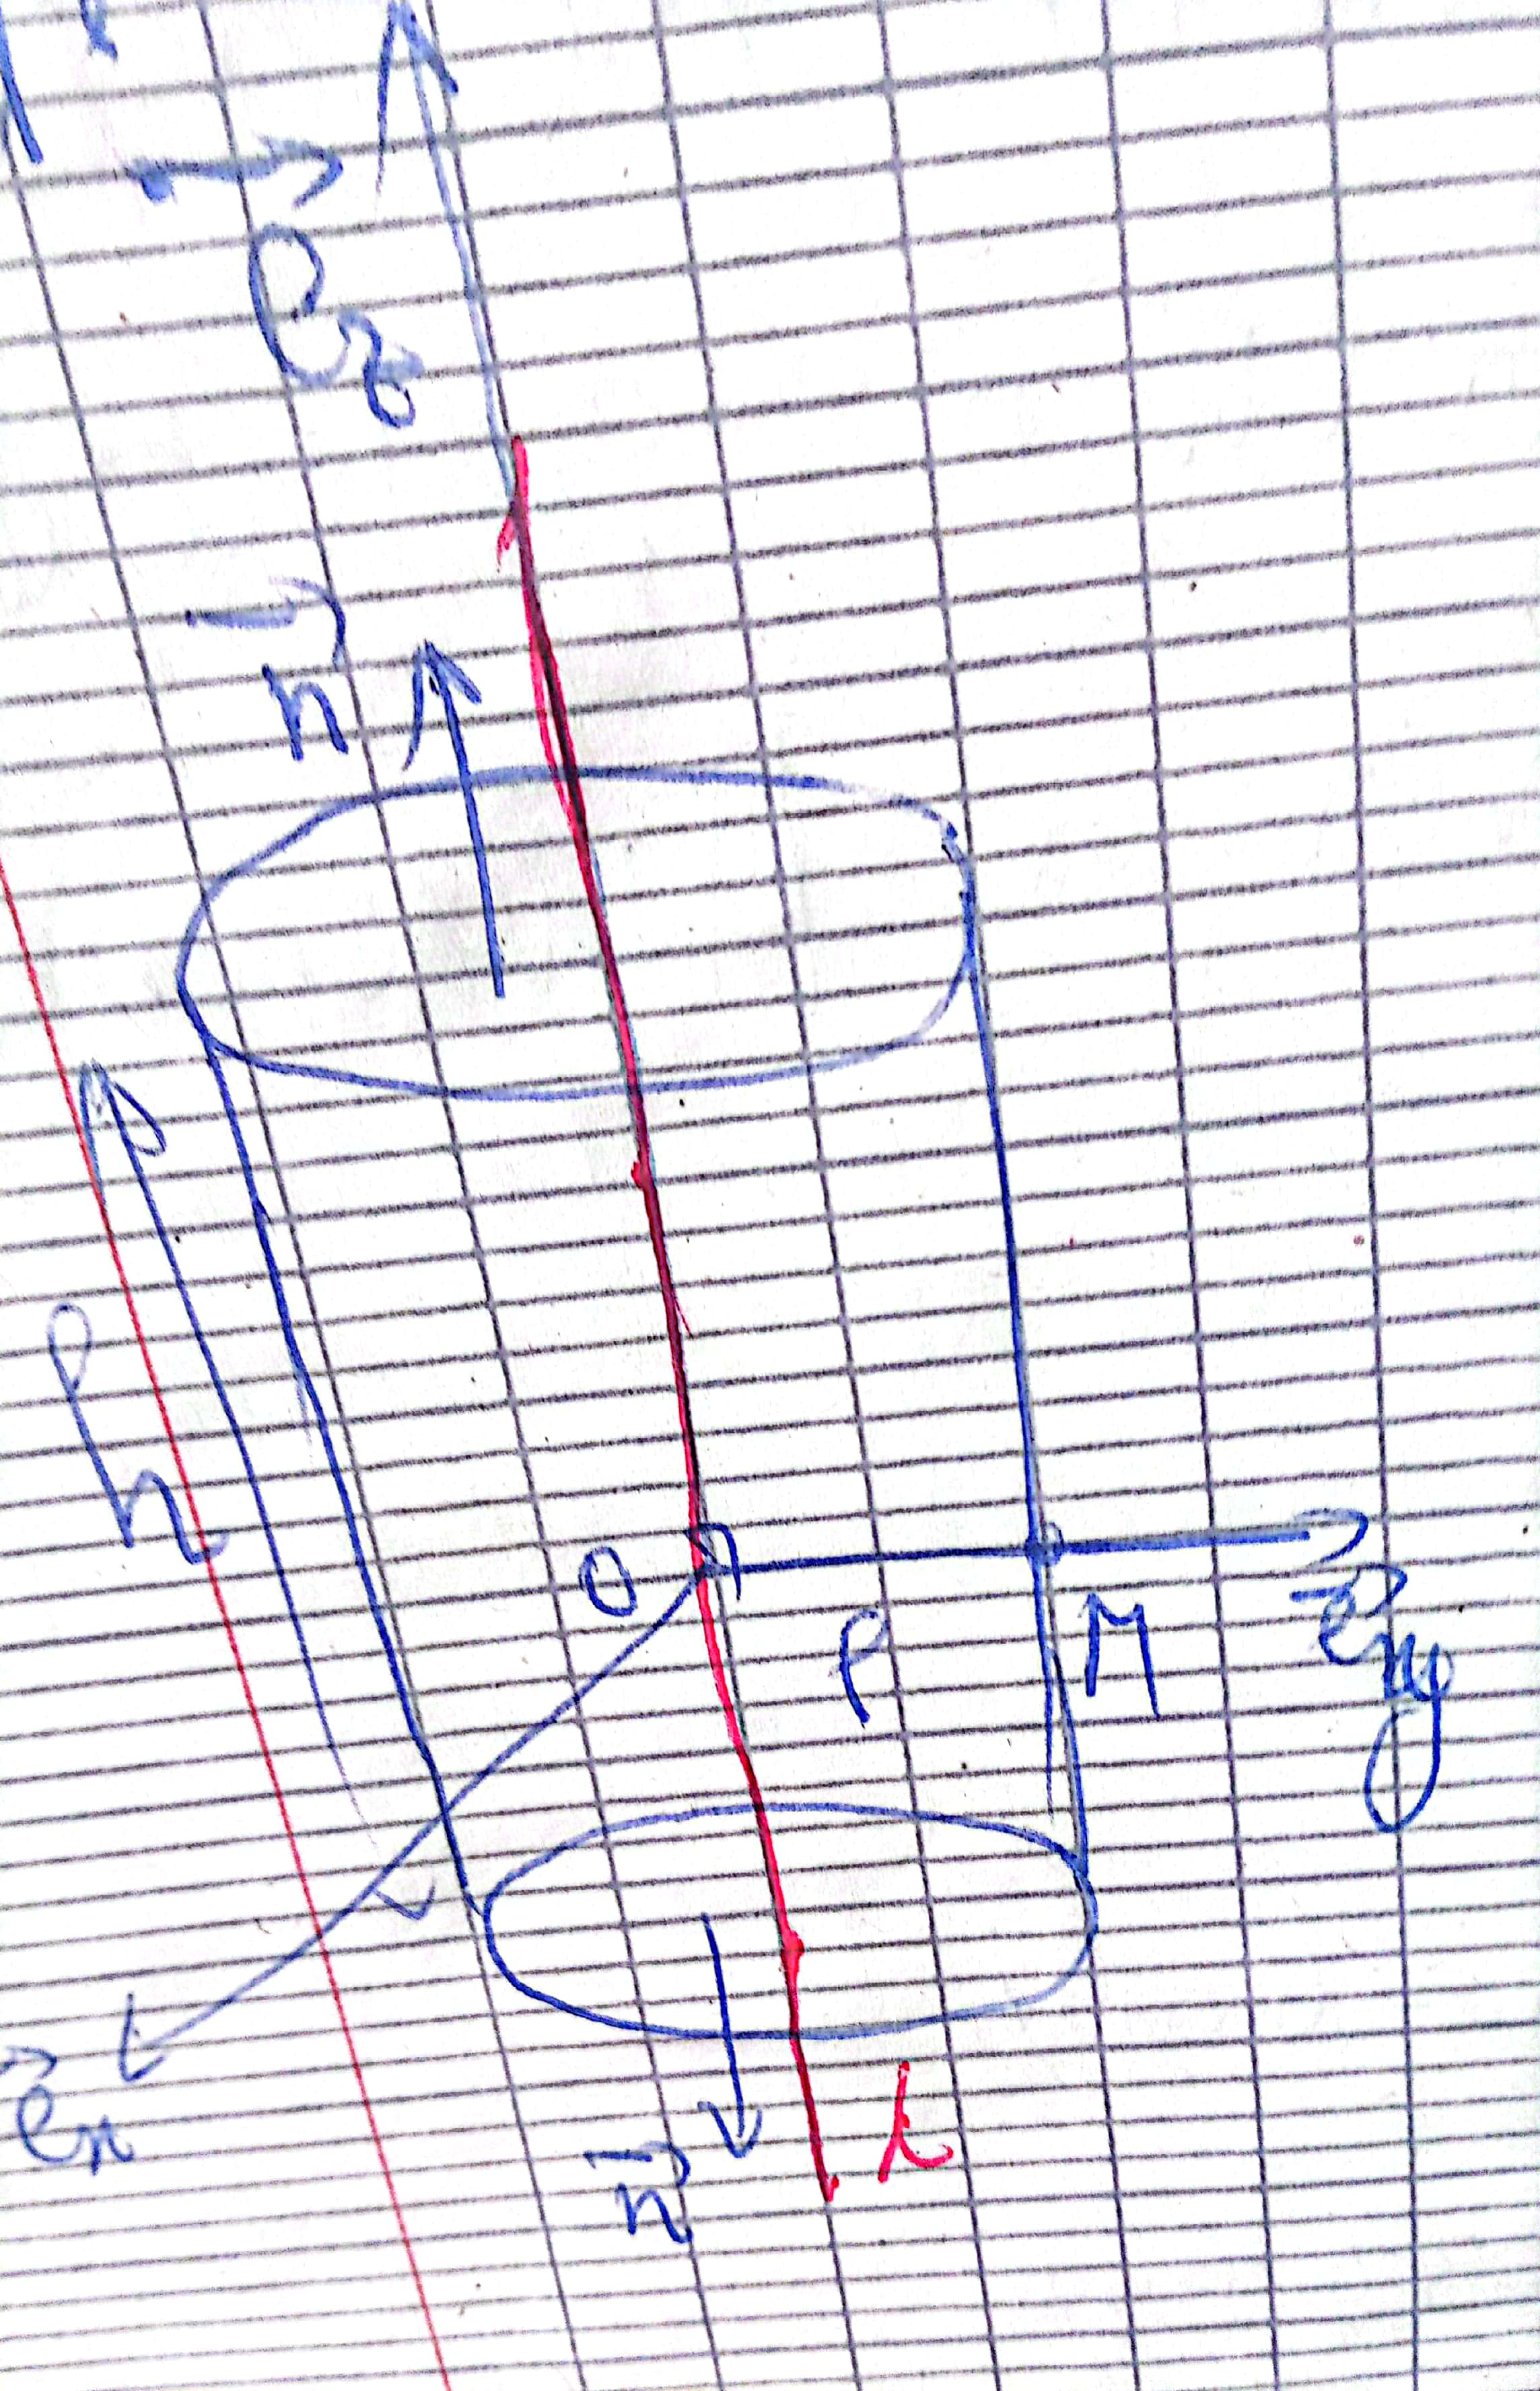
\includegraphics[width=0.7\textwidth]{images/electrostatique/elecst-012-005.png}
\captionof{figure}{\small Plan infini chargé : cylindre de Gauss « pilulier » traversant le plan, champ $\vec{E}$ perpendiculaire au plan.}
\end{center}
\end{boitecorrige}

\subsection*{Exercice 17 - Fil infini et force magnétique \niveau{\moyen}}

\begin{boiteexercice}
Un fil rectiligne infini est parcouru par un courant $I = \qty{10}{A}$.
\begin{enumerate}
  \item Calculer le champ magnétique $B$ à la distance $r = \qty{5}{cm}$ : $B = \mu_0 I/(2\pi r)$.
  \item Un second fil parallèle, de longueur $L = \qty{20}{cm}$, parcouru par $I' = \qty{5}{A}$, est placé à la même distance $r = \qty{5}{cm}$ du premier. Calculer la force exercée sur ce second fil.
  \item Les deux fils sont-ils attirés ou repoussés lorsque les courants sont dans le même sens ? dans le sens opposé ?
\end{enumerate}
\textbf{Donnée :} $\mu_0 = 4\pi\times10^{-7}\,\text{H.m}^{-1}$.
\end{boiteexercice}

\begin{boitecorrige}
\textbf{1.} Par le théorème d'Ampère (contour circulaire de rayon $r$) :
\[
B = \frac{\mu_0 I}{2\pi r} = \frac{4\pi\times10^{-7}\times10}{2\pi\times0{,}05} = \frac{4\times10^{-6}}{0{,}1} = \qty{4e-5}{T} = \qty{40}{\mu T}
\]

\textbf{2.} La force par unité de longueur sur un fil de courant $I'$ dans un champ $B$ est $F/L = I'B$. Pour la longueur $L = \qty{0.2}{m}$ :
\[
F = I' B L = 5\times4\times10^{-5}\times0{,}2 = \qty{4e-5}{N}
\]

\textbf{3.}
\begin{itemize}
  \item Courants de \textbf{même sens} : les deux fils s'attirent (force attractive). C'est la base de la définition historique de l'ampère.
  \item Courants de \textbf{sens opposés} : les deux fils se repoussent.
\end{itemize}
\end{boitecorrige}

\subsection*{Exercice 18 - Solénoïde : champ et flux \niveau{\facile}}

\begin{boiteexercice}
Un solénoïde de densité linéique $n = \qty{2000}{spires.m^{-1}}$, de rayon $R = \qty{2}{cm}$, est parcouru par un courant $I = \qty{3}{A}$.
\begin{enumerate}
  \item Calculer le champ magnétique $B = \mu_0 n I$ à l'intérieur du solénoïde.
  \item Calculer le flux magnétique à travers une section transversale : $\Phi = B\cdot\pi R^2$.
  \item Si la longueur du solénoïde est $\ell = \qty{30}{cm}$, donner le nombre total de spires $N = n\ell$ et l'inductance propre $L = N\Phi/I = \mu_0 n^2 \pi R^2 \ell$.
\end{enumerate}
\textbf{Donnée :} $\mu_0 = 4\pi\times10^{-7}\,\text{H.m}^{-1}$.
\end{boiteexercice}

\begin{boitecorrige}
\textbf{1.} Champ à l'intérieur d'un solénoïde infini :
\[
B = \mu_0 n I = 4\pi\times10^{-7}\times2000\times3 = 4\pi\times10^{-7}\times6000 = 24\pi\times10^{-4} \approx \qty{7.54}{mT}
\]

\textbf{2.} Flux à travers une section de rayon $R = \qty{0.02}{m}$ :
\[
\Phi = B\cdot\pi R^2 = 7{,}54\times10^{-3}\times\pi\times(0{,}02)^2 = 7{,}54\times10^{-3}\times\pi\times4\times10^{-4}
\]
\[
\Phi = 7{,}54\times10^{-3}\times1{,}257\times10^{-3} \approx \qty{9.47e-6}{Wb}
\]

\textbf{3.} Nombre de spires : $N = n\ell = 2000\times0{,}3 = 600\,\text{spires}$.

Inductance propre :
\[
L = \frac{N\Phi}{I} = \frac{600\times9{,}47\times10^{-6}}{3} = \frac{5{,}682\times10^{-3}}{3} \approx \qty{1.89}{mH}
\]
Vérification par la formule directe : $L = \mu_0 n^2\pi R^2\ell = 4\pi\times10^{-7}\times(2000)^2\times\pi\times(0{,}02)^2\times0{,}3 \approx \qty{1.89}{mH}$.
\end{boitecorrige}


\subsection*{Exercice 19 - Dipôle électrique : champ et potentiel \niveau{\difficile}}

\begin{boiteexercice}
Un dipôle électrique est formé de deux charges $+q$ et $-q$ séparées d'une distance $d$. On définit le moment dipolaire $\vec{p} = q\vec{d}$, dirigé de $-q$ vers $+q$, de module $p = qd$.

On travaille en coordonnées sphériques $(r, \theta)$ où $\theta$ est l'angle entre $\vec{r}$ et l'axe du dipôle, et on suppose $r \gg d$ (approximation dipolaire).

\begin{enumerate}
  \item Le potentiel électrostatique créé par le dipôle à grande distance est :
  \[
  V(r,\theta) = \frac{p\cos\theta}{4\pi\varepsilon_0\,r^2}
  \]
  Vérifier la cohérence dimensionnelle de cette expression.

  \item Les composantes du champ électrique $\vec{E} = -\overrightarrow{\text{grad}}\,V$ en coordonnées sphériques sont :
  \[
  E_r = -\frac{\partial V}{\partial r} = \frac{2p\cos\theta}{4\pi\varepsilon_0\,r^3}, \qquad
  E_\theta = -\frac{1}{r}\frac{\partial V}{\partial\theta} = \frac{p\sin\theta}{4\pi\varepsilon_0\,r^3}
  \]
  Calculer $E_r$ et $E_\theta$ à partir de $V$.

  \item Application numérique : pour une molécule d'eau ($p = \qty{6.2e-30}{C.m}$), calculer $V$ et $|\vec{E}|$ à $r = \qty{1}{nm}$ selon $\theta = 0^\circ $ et $\theta = 90^\circ $.

  \item Un dipôle $\vec{p}$ est placé dans un champ électrique extérieur uniforme $\vec{E}_0$. L'énergie potentielle d'interaction est $U = -\vec{p}\cdot\vec{E}_0$. Calculer $U$ pour $p = \qty{6.2e-30}{C.m}$ et $E_0 = \qty{1e6}{V.m^{-1}}$ pour $\theta = 0^\circ $ (dipôle aligné avec le champ) et $\theta = 90^\circ $ (dipôle perpendiculaire).

  \item Quelle est la position d'équilibre stable du dipôle dans le champ ? Justifier.
\end{enumerate}

\textbf{Données :} $\varepsilon_0 = \qty{8.85e-12}{F.m^{-1}}$, $k = 1/(4\pi\varepsilon_0) = \qty{9e9}{N.m^2.C^{-2}}$.
\end{boiteexercice}

\begin{boitecorrige}
\textbf{1. Vérification dimensionnelle.}

$[p] = \text{C}\cdot\text{m}$, $[4\pi\varepsilon_0] = \text{F.m}^{-1}\cdot\text{m} = \text{C}^2/(\text{J}\cdot\text{m}) \cdot\text{m} = \text{C}^2/\text{J}$.

\[
[V] = \frac{[\text{C}\cdot\text{m}]}{[\text{C}^2/\text{J}]\cdot[\text{m}^2]} = \frac{\text{C}\cdot\text{m}\cdot\text{J}}{\text{C}^2\cdot\text{m}^2} = \frac{\text{J}}{\text{C}\cdot\text{m}} = \frac{\text{V}}{\text{m}} \times\text{m} = \ldots
\]

On vérifie plus directement : $[p\cos\theta/(4\pi\varepsilon_0 r^2)] = \frac{\text{C}\cdot\text{m}}{\text{F.m}^{-1}\cdot\text{m}^2\cdot\text{m}} = \frac{\text{C}}{\text{F}} = \frac{\text{C}}{\text{C/V}} = \text{V}$.

\textbf{2. Calcul du champ.}

\textit{Composante radiale :}
\[
E_r = -\frac{\partial V}{\partial r} = -\frac{\partial}{\partial r}\left(\frac{p\cos\theta}{4\pi\varepsilon_0\,r^2}\right) = -p\cos\theta\cdot\frac{-2}{4\pi\varepsilon_0\,r^3} = \frac{2p\cos\theta}{4\pi\varepsilon_0\,r^3}
\]

\textit{Composante angulaire :}
\[
E_\theta = -\frac{1}{r}\frac{\partial V}{\partial\theta} = -\frac{1}{r}\cdot\frac{p}{4\pi\varepsilon_0\,r^2}\cdot(-\sin\theta) = \frac{p\sin\theta}{4\pi\varepsilon_0\,r^3}
\]

Le module du champ est :
\[
|\vec{E}| = \sqrt{E_r^2 + E_\theta^2} = \frac{p}{4\pi\varepsilon_0\,r^3}\sqrt{4\cos^2\theta + \sin^2\theta} = \frac{p}{4\pi\varepsilon_0\,r^3}\sqrt{1 + 3\cos^2\theta}
\]

\textbf{3. Application numérique} ($p = \qty{6.2e-30}{C.m}$, $r = \qty{1}{nm} = \qty{1e-9}{m}$, $k = \qty{9e9}{N.m^2.C^{-2}}$).

\textit{Selon $\theta = 0^\circ $ (axe du dipôle) :}
\[
V = \frac{kp\cos 0^\circ }{r^2} = \frac{9\times10^9\times6{,}2\times10^{-30}}{(10^{-9})^2} = \frac{5{,}58\times10^{-20}}{10^{-18}} \approx \qty{0.0558}{V}
\]
\[
|\vec{E}| = \frac{kp\sqrt{1+3}}{r^3} = \frac{9\times10^9\times6{,}2\times10^{-30}\times2}{10^{-27}} = \frac{1{,}116\times10^{-19}}{10^{-27}} \approx \qty{1.116e8}{V.m^{-1}}
\]

\textit{Selon $\theta = 90^\circ $ (plan équatorial) :}
\[
V = \frac{kp\cos 90^\circ }{r^2} = 0
\]
\[
|\vec{E}| = \frac{kp\sqrt{0+1}}{r^3} = \frac{9\times10^9\times6{,}2\times10^{-30}}{10^{-27}} = \qty{5.58e7}{V.m^{-1}}
\]
Le champ dans le plan équatorial est deux fois plus faible que sur l'axe.

\textbf{4. Énergie d'interaction.}

$U = -\vec{p}\cdot\vec{E}_0 = -pE_0\cos\theta$.

\begin{itemize}[nosep]
  \item $\theta = 0^\circ $ : $U = -pE_0 = -6{,}2\times10^{-30}\times10^6 = \qty{-6.2e-24}{J}$ (état de basse énergie).
  \item $\theta = 90^\circ $ : $U = 0$ (dipôle perpendiculaire, état d'énergie nulle).
\end{itemize}

\textbf{5. Position d'équilibre stable.}

L'équilibre stable correspond au minimum d'énergie potentielle $U = -pE_0\cos\theta$, soit $\cos\theta = +1$, c'est-à-dire $\theta = 0^\circ $ : le dipôle est aligné avec le champ ($\vec{p}$ parallèle à $\vec{E}_0$). C'est intuitivement cohérent : le champ tend à aligner les dipôles dans sa direction (c'est le phénomène de polarisation des diélectriques). À $\theta = 180^\circ $ ($\vec{p}$ antiparallèle à $\vec{E}_0$), l'énergie est maximale : c'est un équilibre instable.

\begin{center}
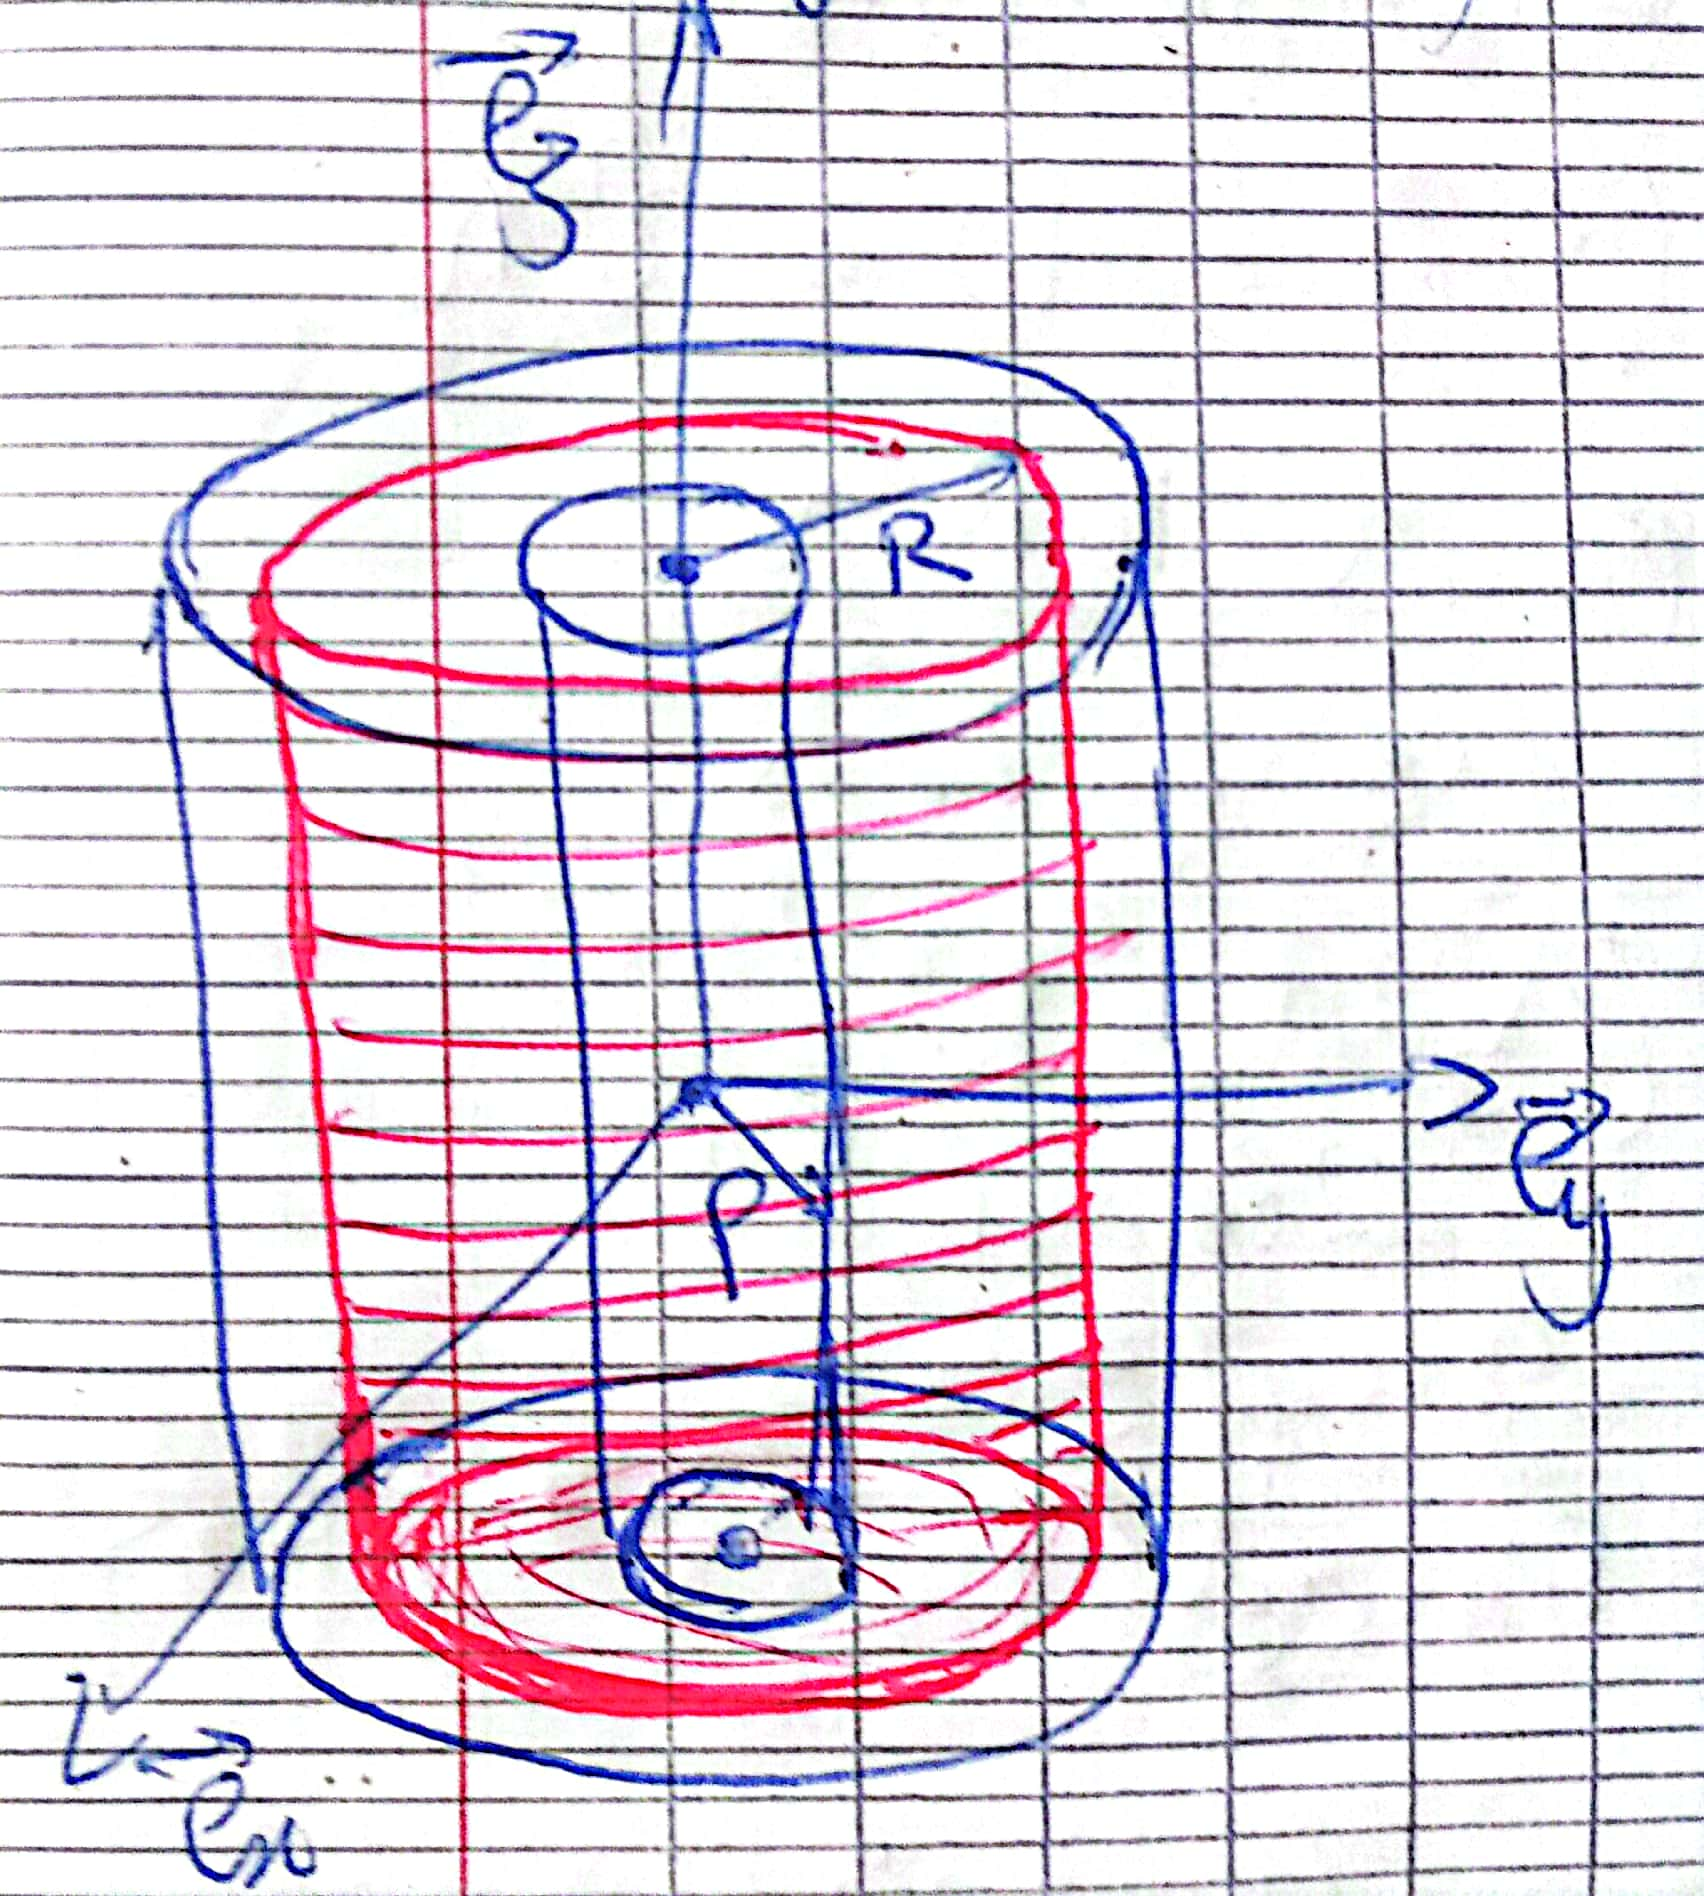
\includegraphics[width=0.7\textwidth]{images/electrostatique/elecst-013-007.png}
\captionof{figure}{\small Dipôle électrique : lignes de champ émanant de $+q$ et convergeant vers $-q$, moment dipolaire $\vec{p}$.}
\end{center}
\end{boitecorrige}

\subsection*{Exercice 20 - Énergie électrostatique d'une sphère chargée \niveau{\difficile}}

\begin{boiteexercice}
On considère une sphère conductrice de rayon $R$ portant une charge totale $Q$ répartie uniformément en surface.

\begin{enumerate}
  \item Rappeler le champ électrique $\vec{E}$ à l'intérieur ($r < R$) et à l'extérieur ($r > R$) de la sphère.
  \item L'énergie électrostatique stockée dans le champ peut se calculer par :
  \[
  U_E = \frac{\varepsilon_0}{2}\int_{\text{tout l'espace}} E^2\,\d^3r
  \]
  En intégrant sur tout l'espace, montrer que :
  \[
  U_E = \frac{Q^2}{8\pi\varepsilon_0 R}
  \]
  \item Application numérique pour une sphère de $R = \qty{10}{cm}$ portant $Q = \qty{1}{\mu C}$.
  \item À quelle tension équivalente de condensateur sphérique $C = 4\pi\varepsilon_0 R$ correspond cette énergie ($U_E = Q^2/(2C)$) ?
\end{enumerate}
\end{boiteexercice}

\begin{boitecorrige}
\textbf{1. Champ électrique.}

Pour une sphère conductrice, les charges se répartissent en surface. Par le théorème de Gauss :
\[
E(r < R) = 0 \quad \text{(intérieur d'un conducteur)}
\]
\[
E(r > R) = \frac{Q}{4\pi\varepsilon_0\,r^2} \quad \text{(identique à une charge ponctuelle)}
\]

\textbf{2. Calcul de l'énergie.}

Comme $E = 0$ à l'intérieur, seule la région extérieure ($r > R$) contribue. En coordonnées sphériques, $\d^3r = 4\pi r^2\,\d r$ :
\[
U_E = \frac{\varepsilon_0}{2}\int_R^{+\infty} E^2(r)\cdot 4\pi r^2\,\d r = \frac{\varepsilon_0}{2}\int_R^{+\infty} \left(\frac{Q}{4\pi\varepsilon_0\,r^2}\right)^2 4\pi r^2\,\d r
\]
\[
= \frac{\varepsilon_0}{2}\cdot\frac{Q^2}{16\pi^2\varepsilon_0^2}\cdot 4\pi\int_R^{+\infty} \frac{1}{r^4}\cdot r^2\,\d r = \frac{Q^2}{8\pi\varepsilon_0}\int_R^{+\infty} r^{-2}\,\d r
\]
\[
= \frac{Q^2}{8\pi\varepsilon_0}\left[\frac{-1}{r}\right]_R^{+\infty} = \frac{Q^2}{8\pi\varepsilon_0}\cdot\frac{1}{R}
\]
\[
\boxed{U_E = \frac{Q^2}{8\pi\varepsilon_0 R}}
\]

\textbf{3. Application numérique.}

\[
U_E = \frac{Q^2}{8\pi\varepsilon_0 R} = k\frac{Q^2}{2R} = \frac{9\times10^9\times(10^{-6})^2}{2\times0{,}1} = \frac{9\times10^9\times10^{-12}}{0{,}2} = \qty{45}{mJ}
\]

\textbf{4. Capacité et tension.}

La capacité d'une sphère isolée : $C = 4\pi\varepsilon_0 R = \dfrac{R}{k} = \dfrac{0{,}1}{9\times10^9} \approx \qty{11.1}{pF}$.

La relation $U_E = Q^2/(2C)$ donne :
\[
U_E = \frac{(10^{-6})^2}{2\times11{,}1\times10^{-12}} = \frac{10^{-12}}{22{,}2\times10^{-12}} \approx \qty{45}{mJ}
\]

La tension correspondante est :
\[
V = \frac{Q}{C} = \frac{kQ}{R} = \frac{9\times10^9\times10^{-6}}{0{,}1} = \qty{90000}{V} = \qty{90}{kV}
\]
Une sphère de $10\,\text{cm}$ de rayon portant $1\,\mu\text{C}$ est portée à $90\,\text{kV}$ --- cela illustre pourquoi des charges macroscopiques sur de petits objets produisent des tensions très élevées.
\end{boitecorrige}

\ifdefined\inMainDoc\else\end{document}\fi


% ================================================================
%  UE 8 : LOGIQUE ET ALGÈBRE DE BASE
% ================================================================
\newpage
\thispagestyle{empty}
\begin{tikzpicture}[remember picture, overlay]
  \fill[gray!12] ([xshift=1.5cm, yshift=3cm]current page.south west)
    rectangle ([xshift=-1.5cm, yshift=-3cm]current page.north east);
  \draw[line width=3pt] ([xshift=1.5cm,yshift=-3cm]current page.north west)
    -- ([xshift=-1.5cm,yshift=-3cm]current page.north east);
  \draw[line width=3pt] ([xshift=1.5cm,yshift=3cm]current page.south west)
    -- ([xshift=-1.5cm,yshift=3cm]current page.south east);
  \node[align=center] at (current page.center) {%
    {\fontsize{28}{36}\bfseries\selectfont LOGIQUE ET ALGÈBRE DE BASE}\\[1.2cm]
    {\large\itshape Logique propositionnelle - Théorie des ensembles}\\[0.4cm]
    {\large\itshape Relations - Applications - Algèbre de Boole}\\[1.8cm]
    {\normalsize Licence 1 - UE 8}
  };
  \node[anchor=south west] at ([xshift=2cm,yshift=2cm]current page.south west)
    {\large\bfseries UE 8};
\end{tikzpicture}
\newpage

\addcontentsline{toc}{section}{LOGIQUE ET ALGÈBRE DE BASE}
\ifdefined\inMainDoc\else
\documentclass[12pt,a4paper]{article}
% ================================================================
%  PRÉAMBULE COMMUN - ANNALES CORRIGÉES
%  Université de Kara - FaST - Licence Fondamentale MPC
%  Design optimisé impression noir et blanc
% ================================================================

% -- ENCODAGE & LANGUE --
\usepackage[utf8]{inputenc}
\usepackage[T1]{fontenc}
\usepackage[french]{babel}
\usepackage{lmodern}
\usepackage{microtype}

% -- MISE EN PAGE --
\usepackage[a4paper, top=2.8cm, bottom=2.5cm, left=2.5cm, right=2.5cm, headheight=14pt]{geometry}
\usepackage{setspace}
\setstretch{1.2}
\usepackage{parskip}
\setlength{\parindent}{1.2em}
\setlength{\parskip}{4pt}

% -- MATHS --
\usepackage{amsmath, amssymb, mathtools, amsthm}
\usepackage{mathrsfs}
\usepackage{dsfont}
\usepackage{bm}
\usepackage{cancel}
\usepackage{textcomp}
% Définition de \oiint (intégrale de surface fermée) sans package supplémentaire
\newcommand{\oiint}{\mathop{\iint\!\!\!\!\!\!\!\bigcirc}\limits}

% -- PHYSIQUE & CHIMIE --
\usepackage{physics}
\usepackage{siunitx}
% Lorsque physics est chargé, siunitx omet \qty. On le restaure ici :
\AtBeginDocument{\RenewCommandCopy\qty\SI}
\sisetup{locale = FR, detect-all, output-decimal-marker={,}}
% Commande de substitution pour les unités posant problème avec pdflatex
% (ohm, degreeCelsius, micro, angstrom, percent utilisent des caractères non-ASCII)
\newcommand{\qtyohm}[1]{\ensuremath{\num{#1}\,\Omega}}
\newcommand{\qtydegc}[1]{\ensuremath{\num{#1}\,{}^\circ\text{C}}}
\newcommand{\qtyangstrom}[1]{\ensuremath{\num{#1}\,\text{\AA}}}
\newcommand{\qtypercent}[1]{\ensuremath{\num{#1}\,\%}}
\newcommand{\qtyum}[1]{\ensuremath{\num{#1}\,\mu\text{m}}}
\usepackage[version=4]{mhchem}

% -- GRAPHISMES --
\usepackage{graphicx}
\usepackage{float}
\usepackage{caption}
\usepackage{subcaption}
\usepackage{wrapfig}
\usepackage{tikz}
\usetikzlibrary{calc, arrows.meta, patterns, shapes.geometric}
\usepackage{pgfplots}
\pgfplotsset{compat=1.18}

% -- TABLEAUX --
\usepackage{booktabs}
\usepackage{array}
\usepackage{tabularx}
\usepackage{multirow}

% -- LISTES --
\usepackage{enumitem}
\setlist[enumerate]{topsep=3pt, itemsep=2pt, parsep=0pt}
\setlist[itemize]{topsep=3pt, itemsep=2pt, parsep=0pt, label={.}}

% -- BOÎTES (noir et blanc) --
\usepackage{mdframed}
\usepackage{tcolorbox}
\tcbuselibrary{skins, breakable, theorems}

% Boîte EXERCICE : encadré avec filet épais, fond blanc
\newmdenv[
  linewidth=1.2pt,
  linecolor=black,
  roundcorner=3pt,
  skipabove=10pt,
  skipbelow=6pt,
  innertopmargin=8pt,
  innerbottommargin=8pt,
  innerleftmargin=10pt,
  innerrightmargin=10pt,
  backgroundcolor=white,
  frametitle={\bfseries\small Exercice},
  frametitlealignment=\raggedright,
  frametitleaboveskip=4pt,
  frametitlebelowskip=4pt,
]{boiteexercice}

% Boîte CORRIGÉ : fond gris très clair + filet fin
\newmdenv[
  linewidth=0.6pt,
  linecolor=black,
  leftline=true,
  rightline=false,
  topline=false,
  bottomline=false,
  linecolor=black,
  innerleftmargin=12pt,
  innerrightmargin=8pt,
  innertopmargin=6pt,
  innerbottommargin=6pt,
  backgroundcolor=gray!8,
  skipabove=4pt,
  skipbelow=8pt,
]{boitecorrige}

% Boîte RÉSUMÉ DE COURS : double encadré
\newmdenv[
  linewidth=0.8pt,
  linecolor=black,
  roundcorner=2pt,
  backgroundcolor=gray!12,
  innertopmargin=10pt,
  innerbottommargin=10pt,
  innerleftmargin=12pt,
  innerrightmargin=12pt,
  skipabove=12pt,
  skipbelow=8pt,
]{boiteresume}

% Boîte ATTENTION/REMARQUE : barre gauche épaisse
\newmdenv[
  leftline=true,
  rightline=false,
  topline=false,
  bottomline=false,
  linewidth=3pt,
  linecolor=black,
  backgroundcolor=gray!5,
  innerleftmargin=12pt,
  innerrightmargin=8pt,
  innertopmargin=5pt,
  innerbottommargin=5pt,
  skipabove=6pt,
  skipbelow=6pt,
]{boiteremarque}

% -- DIFFICULTÉ DES EXERCICES --
\newcommand{\facile}{$\star$}
\newcommand{\moyen}{$\star\!\star$}
\newcommand{\difficile}{$\star\!\star\!\star$}
\newcommand{\niveau}[1]{\hfill\textbf{#1}\hspace{2pt}}

% -- EN-TÊTES ET PIEDS DE PAGE --
\usepackage{fancyhdr}
\pagestyle{fancy}
\fancyhf{}
\renewcommand{\headrulewidth}{0.5pt}
\renewcommand{\footrulewidth}{0.3pt}

% -- HYPERLIENS --
\usepackage[hidelinks]{hyperref}
\hypersetup{
    colorlinks=false,
    pdftitle={Annale Corrigée - Licence MPC - Université de Kara}
}

% -- TITRES --
\usepackage{titlesec}
\titleformat{\section}{\Large\bfseries}{\thesection.}{0.8em}{}[\vspace{2pt}\hrule\vspace{4pt}]
\titleformat{\subsection}{\large\bfseries}{\thesubsection.}{0.7em}{}
\titleformat{\subsubsection}{\normalsize\bfseries}{\thesubsubsection.}{0.6em}{}

% -- THÉORÈMES --
\theoremstyle{definition}
\newtheorem{defn}{Définition}[section]
\newtheorem{prop}{Propriété}[section]
\newtheorem{thm}{Théorème}[section]
\newtheorem{corol}{Corollaire}[section]
\newtheorem{exemple}{Exemple}[section]

% -- COMMANDES MATHÉMATIQUES UTILES --
\newcommand{\vect}[1]{\overrightarrow{#1}}
\newcommand{\R}{\mathbb{R}}
\newcommand{\N}{\mathbb{N}}
\newcommand{\Z}{\mathbb{Z}}
\newcommand{\C}{\mathbb{C}}
\renewcommand{\d}{\mathrm{d}}
\newcommand{\deriv}[2]{\dfrac{\d #1}{\d #2}}
\newcommand{\dpart}[2]{\dfrac{\partial #1}{\partial #2}}
\newcommand{\rot}{\overrightarrow{\mathrm{rot}}\,}
\renewcommand{\div}{\mathrm{div}\,}
\renewcommand{\grad}{\overrightarrow{\mathrm{grad}}\,}
\newcommand{\e}{\mathrm{e}}
\newcommand{\ii}{\mathrm{i}}
\renewcommand{\Tr}{\mathrm{Tr}}

% Numérotation des équations par section
\numberwithin{equation}{section}

% -- RÉSULTATS ENCADRÉS --
\newcommand{\res}[1]{\[\boxed{#1}\]}

% -- REMARQUE INLINE --
\newcommand{\rmq}[1]{\begin{boiteremarque}\textbf{Remarque.} #1\end{boiteremarque}}

% -- MISE EN VALEUR DU RÉSULTAT FINAL --
\newcommand{\reponse}[1]{%
  \begin{center}
    \fbox{\begin{minipage}{0.92\textwidth}\centering #1\end{minipage}}
  \end{center}%
}


\lhead{\small\textit{Logique et Algèbre de Base - Licence 1}}
\rhead{\small\textit{FaST, Université de Kara}}
\cfoot{\thepage}

\begin{document}
\fi

\begin{center}
  {\LARGE\bfseries LOGIQUE ET ALGÈBRE DE BASE}\\[0.3cm]
  {\normalsize Licence 1 - Mathématiques, Physique et Chimie}\\[0.1cm]
  \rule{0.7\textwidth}{0.8pt}
\end{center}

\section*{Résumé du cours}

\begin{boiteresume}

\textbf{1. Propositions et connecteurs logiques.} Une \textit{proposition} est un énoncé vrai (V) ou faux (F). Les connecteurs : négation $\neg p$, conjonction $p\wedge q$ (ET), disjonction $p\vee q$ (OU), implication $p\Rightarrow q$ (équivalente à $\neg p\vee q$), équivalence $p\Leftrightarrow q$.

Lois de De Morgan : $\neg(p\wedge q)\equiv\neg p\vee\neg q$ et $\neg(p\vee q)\equiv\neg p\wedge\neg q$.

\textbf{2. Tables de vérité.}
\begin{center}
\begin{tabular}{cc|cccc}
$p$ & $q$ & $p\wedge q$ & $p\vee q$ & $p\Rightarrow q$ & $p\Leftrightarrow q$\\
\hline
V & V & V & V & V & V\\
V & F & F & V & F & F\\
F & V & F & V & V & F\\
F & F & F & F & V & V\\
\end{tabular}
\end{center}

\textbf{3. Ensembles.} Opérations : union $A\cup B$, intersection $A\cap B$, différence $A\setminus B$, complémentaire $\bar{A}$. Lois de De Morgan pour les ensembles : $\overline{A\cup B}=\bar{A}\cap\bar{B}$, $\overline{A\cap B}=\bar{A}\cup\bar{B}$.

\textbf{4. Relations.} Une relation $\mathcal{R}$ sur $E$ est réflexive ($a\mathcal{R}a$), symétrique ($a\mathcal{R}b\Rightarrow b\mathcal{R}a$), transitive ($a\mathcal{R}b$ et $b\mathcal{R}c\Rightarrow a\mathcal{R}c$), antisymétrique ($a\mathcal{R}b$ et $b\mathcal{R}a\Rightarrow a=b$). Une \textit{relation d'équivalence} est réflexive, symétrique et transitive.

\textbf{5. Applications.} Une application $f:A\to B$ est injective si $f(x)=f(y)\Rightarrow x=y$, surjective si $\forall y\in B,\;\exists x\in A:f(x)=y$, bijective si elle est injective et surjective.

\textbf{6. Algèbre de Boole.} Un treillis booléen $(B,+,\cdot,\bar{\phantom{x}},0,1)$ avec les lois : commutativité, associativité, distributivité, identité ($a+0=a$, $a\cdot1=a$), complémentation ($a+\bar{a}=1$, $a\cdot\bar{a}=0$).

\end{boiteresume}

\newpage
\section{Logique propositionnelle}

\subsection*{Exercice 1 - Tables de vérité \niveau{\facile}}

\begin{boiteexercice}
\begin{enumerate}
  \item Construire la table de vérité de $p\Rightarrow(q\wedge r)$.
  \item Construire la table de vérité de $(p\Rightarrow q)\wedge(q\Rightarrow r)$ et de $p\Rightarrow r$. Ces deux formules sont-elles équivalentes ?
  \item Montrer que $\neg(p\Rightarrow q)\equiv p\wedge\neg q$.
\end{enumerate}
\end{boiteexercice}

\begin{boitecorrige}
\textbf{1.}
\begin{center}
\begin{tabular}{ccc|cc|c}
$p$ & $q$ & $r$ & $q\wedge r$ & $p\Rightarrow(q\wedge r)$\\
\hline
V & V & V & V & V\\
V & V & F & F & F\\
V & F & V & F & F\\
V & F & F & F & F\\
F & V & V & V & V\\
F & V & F & F & V\\
F & F & V & F & V\\
F & F & F & F & V\\
\end{tabular}
\end{center}

\textbf{2.}
\begin{center}
\begin{tabular}{ccc|cc|cc|c}
$p$ & $q$ & $r$ & $p\Rightarrow q$ & $q\Rightarrow r$ & $(p\Rightarrow q)\wedge(q\Rightarrow r)$ & $p\Rightarrow r$\\
\hline
V & V & V & V & V & V & V\\
V & V & F & V & F & F & F\\
V & F & V & F & V & F & V\\
V & F & F & F & V & F & F\\
F & V & V & V & V & V & V\\
F & V & F & V & F & F & V\\
F & F & V & V & V & V & V\\
F & F & F & V & V & V & V\\
\end{tabular}
\end{center}
Les colonnes diffèrent (ligne 3) : les formules ne sont \textbf{pas} équivalentes. Mais $(p\Rightarrow q)\wedge(q\Rightarrow r)\Rightarrow(p\Rightarrow r)$ est une tautologie (principe de transitivité).

\textbf{3.} $\neg(p\Rightarrow q) = \neg(\neg p\vee q) = p\wedge\neg q$ (De Morgan). Table de vérité :
\begin{center}
\begin{tabular}{cc|c|c|c}
$p$ & $q$ & $p\Rightarrow q$ & $\neg(p\Rightarrow q)$ & $p\wedge\neg q$\\
\hline
V & V & V & F & F\\
V & F & F & V & V\\
F & V & V & F & F\\
F & F & V & F & F\\
\end{tabular}
\end{center}
Les colonnes 4 et 5 sont identiques : $\neg(p\Rightarrow q)\equiv p\wedge\neg q$. En clair, une implication est fausse si et seulement si la prémisse est vraie et la conclusion est fausse.
\end{boitecorrige}

\section{Théorie des ensembles}

\subsection*{Exercice 2 - Opérations sur les ensembles \niveau{\facile}}

\begin{boiteexercice}
Soient $E=\{1,2,3,4,5,6,7,8\}$, $A=\{1,2,3,4\}$, $B=\{3,4,5,6\}$, $C=\{5,6,7,8\}$.
\begin{enumerate}
  \item Calculer $A\cup B$, $A\cap B$, $A\setminus B$, $B\setminus A$, $\bar{A}$.
  \item Vérifier les lois de De Morgan : $\overline{A\cup B}=\bar{A}\cap\bar{B}$.
  \item Calculer $(A\cup B)\cap C$ et $A\cup(B\cap C)$.
\end{enumerate}
\end{boiteexercice}

\begin{boitecorrige}
\textbf{1.}
$A\cup B = \{1,2,3,4,5,6\}$, $A\cap B = \{3,4\}$, $A\setminus B=\{1,2\}$, $B\setminus A=\{5,6\}$, $\bar{A}=\{5,6,7,8\}$.

\textbf{2.} $\overline{A\cup B}=\overline{\{1,2,3,4,5,6\}}=\{7,8\}$.

$\bar{A}\cap\bar{B} = \{5,6,7,8\}\cap\{1,2,7,8\} = \{7,8\}$.

\textbf{3.} $(A\cup B)\cap C = \{1,2,3,4,5,6\}\cap\{5,6,7,8\} = \{5,6\}$.

$A\cup(B\cap C) = \{1,2,3,4\}\cup(\{3,4,5,6\}\cap\{5,6,7,8\}) = \{1,2,3,4\}\cup\{5,6\} = \{1,2,3,4,5,6\}$.

Ces deux résultats sont différents, ce qui illustre que l'union et l'intersection ne sont pas interchangeables dans la distributivité.
\end{boitecorrige}

\subsection*{Exercice 3 - Relations d'équivalence \niveau{\moyen}}

\begin{boiteexercice}
\begin{enumerate}
  \item Sur $\mathbb{Z}$, on définit $a\mathcal{R}b$ si et seulement si $3\mid(a-b)$. Vérifier que $\mathcal{R}$ est une relation d'équivalence et décrire les classes d'équivalence.
  \item Sur $\mathbb{R}$, on définit $x\mathcal{S}y$ si et seulement si $x-y\in\mathbb{Q}$. Montrer que $\mathcal{S}$ est une relation d'équivalence.
  \item Sur $\mathbb{N}^*\times\mathbb{N}^*$, on définit $(a,b)\mathcal{T}(c,d)$ si $ad=bc$. Vérifier que $\mathcal{T}$ est une relation d'équivalence. Que représentent les classes d'équivalence ?
\end{enumerate}
\end{boiteexercice}

\begin{boitecorrige}
\textbf{1.}
\textit{Réflexivité} : $a-a=0=3\times0$, donc $a\mathcal{R}a$.
\textit{Symétrie} : si $3\mid(a-b)$, alors $3\mid(-(a-b))=b-a$, donc $b\mathcal{R}a$.
\textit{Transitivité} : si $a-b=3k$ et $b-c=3l$, alors $a-c=(a-b)+(b-c)=3(k+l)$, donc $a\mathcal{R}c$.

Classes d'équivalence :
\begin{align*}
[0] &= \{\ldots,-6,-3,0,3,6,\ldots\},\\
[1] &= \{\ldots,-5,-2,1,4,7,\ldots\},\\
[2] &= \{\ldots,-4,-1,2,5,8,\ldots\}.
\end{align*}
C'est la congruence modulo 3.

\textbf{2.}
\textit{Réflexivité} : $x-x=0\in\mathbb{Q}$.
\textit{Symétrie} : si $x-y\in\mathbb{Q}$, alors $y-x=-(x-y)\in\mathbb{Q}$.
\textit{Transitivité} : si $x-y\in\mathbb{Q}$ et $y-z\in\mathbb{Q}$, alors $(x-z)=(x-y)+(y-z)\in\mathbb{Q}$.

\textbf{3.}
$(a,b)\mathcal{T}(a,b)$ car $ab=ba$ (réflexivité).
$(a,b)\mathcal{T}(c,d)\Rightarrow ad=bc\Rightarrow cb=da\Rightarrow(c,d)\mathcal{T}(a,b)$.
$(a,b)\mathcal{T}(c,d)$ et $(c,d)\mathcal{T}(e,f)$ : $ad=bc$ et $cf=de$. En multipliant : $adcf=bcde$, donc $af=be$, soit $(a,b)\mathcal{T}(e,f)$.

La classe de $(a,b)$ rassemble tous les couples $(c,d)$ tels que $a/b=c/d$ (même valeur de la fraction). Les classes d'équivalence représentent les \textit{nombres rationnels}.
\end{boitecorrige}

\section{Applications et algèbre de Boole}

\subsection*{Exercice 4 - Injectivité et surjectivité \niveau{\moyen}}

\begin{boiteexercice}
Étudier l'injectivité, la surjectivité et la bijectivité des applications suivantes :
\begin{enumerate}[label=(\alph*)]
  \item $f:\mathbb{R}\to\mathbb{R}$, $f(x)=2x-3$
  \item $g:\mathbb{R}\to\mathbb{R}$, $g(x)=x^2$
  \item $h:\mathbb{R}\to\mathbb{R}^+$, $h(x)=x^2$
  \item $k:\mathbb{R}^+\to\mathbb{R}^+$, $k(x)=x^2$
\end{enumerate}
\end{boiteexercice}

\begin{boitecorrige}
\textbf{(a)} $f(x)=f(y)\Rightarrow 2x-3=2y-3\Rightarrow x=y$ : \textbf{injective}. $\forall y\in\mathbb{R}$, $x=(y+3)/2\in\mathbb{R}$ : \textbf{surjective}. Donc \textbf{bijective}.

\textbf{(b)} $g(1)=g(-1)=1$ : \textbf{non injective}. $g(x)=x^2\geq0$, donc $-1\in\mathbb{R}$ n'a pas d'antécédent : \textbf{non surjective}.

\textbf{(c)} Même non-injectivité que (b) : \textbf{non injective}. Mais maintenant le codomaine est $\mathbb{R}^+$ : $\forall y\geq0$, $h(\sqrt{y})=y$ : \textbf{surjective}.

\textbf{(d)} $k(x)=k(y)$ avec $x,y\geq0$ : $x^2=y^2\Rightarrow(x-y)(x+y)=0$, et comme $x,y\geq0$, $x+y\geq0$, donc $x=y$ : \textbf{injective}. $\forall y\geq0$, $k(\sqrt{y})=y$ : \textbf{surjective}. Donc \textbf{bijective}. La bijection réciproque est $k^{-1}(y)=\sqrt{y}$.
\end{boitecorrige}

\subsection*{Exercice 5 - Algèbre de Boole et simplification \niveau{\difficile}}

\begin{boiteexercice}
En algèbre de Boole, simplifier les expressions suivantes :
\begin{enumerate}[label=(\alph*)]
  \item $A\cdot\bar{A}+B$
  \item $A+(A\cdot B)$
  \item $(A+B)\cdot(A+\bar{B})$
  \item $A\cdot B + A\cdot\bar{B} + \bar{A}\cdot B$
  \item $(A+B)\cdot(\bar{A}+C)\cdot(B+C)$
\end{enumerate}
\end{boiteexercice}

\begin{boitecorrige}
\textbf{(a)} $A\cdot\bar{A}+B = 0+B = B$ (complémentation : $A\cdot\bar{A}=0$).

\textbf{(b)} $A+(A\cdot B) = A\cdot(1+B) = A\cdot1 = A$ (absorption).

\textbf{(c)} $(A+B)(A+\bar{B}) = A+B\cdot\bar{B} = A+0 = A$ (distributivité puis complémentation).

\textbf{(d)} $AB+A\bar{B}+\bar{A}B = A(B+\bar{B})+\bar{A}B = A+\bar{A}B = (A+\bar{A})(A+B) = 1\cdot(A+B) = A+B$.

\textbf{(e)} Par le théorème du consensus, le terme $B+C$ est redondant quand $A+B$ et $\bar{A}+C$ sont tous deux vrais (car si $A=1$ : $B+C$ découle de $\bar{A}+C\Rightarrow C=1$; si $A=0$ : $B+C$ découle de $A+B\Rightarrow B=1$). On montre directement :
$(A+B)(\bar{A}+C)(B+C)$. Développons $(A+B)(\bar{A}+C) = A\bar{A}+AC+\bar{A}B+BC = AC+\bar{A}B+BC$.
En multipliant par $(B+C)$ : $(AC+\bar{A}B+BC)(B+C)$.
$= ACB+ACC+\bar{A}B^2+\bar{A}BC+B^2C+BC^2$
$= ABC+AC+\bar{A}B+\bar{A}BC+BC$
$= AC+\bar{A}B+BC = AC+\bar{A}B+BC$.
Par absorption ($BC$ est couvert par $AC$ et $\bar{A}B$ ensemble) : résultat final $= AC+\bar{A}B$.
\end{boitecorrige}


\subsection*{Exercice 6 - Tautologie et équivalence logique \niveau{\facile}}

\begin{boiteexercice}
\begin{enumerate}
  \item Construire la table de vérité de $(p\Rightarrow q)\Leftrightarrow(\neg p\vee q)$ et montrer que c'est une tautologie.
  \item Construire la table de vérité de $(p\Rightarrow q)\Rightarrow(\neg q\Rightarrow\neg p)$ (contraposée) et montrer que c'est une tautologie.
  \item Montrer que $(p\Leftrightarrow q)\equiv (p\Rightarrow q)\wedge(q\Rightarrow p)$.
\end{enumerate}
\end{boiteexercice}

\begin{boitecorrige}
\textbf{1.}
\begin{center}
\begin{tabular}{cc|c|c|c}
$p$ & $q$ & $p\Rightarrow q$ & $\neg p\vee q$ & $(p\Rightarrow q)\Leftrightarrow(\neg p\vee q)$\\
\hline
V & V & V & V & V\\
V & F & F & F & V\\
F & V & V & V & V\\
F & F & V & V & V\\
\end{tabular}
\end{center}
La dernière colonne est toujours V : c'est bien une \textbf{tautologie}. Cela prouve que $p\Rightarrow q \equiv \neg p\vee q$.

\textbf{2.}
\begin{center}
\begin{tabular}{cc|c|cc|c}
$p$ & $q$ & $p\Rightarrow q$ & $\neg q$ & $\neg q\Rightarrow\neg p$ & $(p\Rightarrow q)\Rightarrow(\neg q\Rightarrow\neg p)$\\
\hline
V & V & V & F & V & V\\
V & F & F & V & F & V\\
F & V & V & F & V & V\\
F & F & V & V & V & V\\
\end{tabular}
\end{center}
Toujours V : tautologie. Cela confirme que $p\Rightarrow q \equiv \neg q\Rightarrow\neg p$ (contraposée).

\textbf{3.} Par définition, $p\Leftrightarrow q$ est vraie quand $p$ et $q$ ont même valeur de vérité. D'autre part, $(p\Rightarrow q)\wedge(q\Rightarrow p)$ est vraie si et seulement si les deux implications sont vraies simultanément, ce qui est le cas uniquement si $p$ et $q$ ont la même valeur. On vérifie dans la table :
\begin{center}
\begin{tabular}{cc|c|c|c|c}
$p$ & $q$ & $p\Rightarrow q$ & $q\Rightarrow p$ & $(p\Rightarrow q)\wedge(q\Rightarrow p)$ & $p\Leftrightarrow q$\\
\hline
V & V & V & V & V & V\\
V & F & F & V & F & F\\
F & V & V & F & F & F\\
F & F & V & V & V & V\\
\end{tabular}
\end{center}
Les colonnes 5 et 6 sont identiques : $p\Leftrightarrow q \equiv (p\Rightarrow q)\wedge(q\Rightarrow p)$.
\end{boitecorrige}

\subsection*{Exercice 7 - Simplification en algèbre de Boole \niveau{\moyen}}

\begin{boiteexercice}
En algèbre de Boole, simplifier la fonction $f = ABC + AB'C + A'BC$.
\begin{enumerate}
  \item Factoriser les deux premiers termes, puis simplifier.
  \item Montrer que la forme minimale est $f = AC + A'BC$.
  \item Vérifier en construisant la table de vérité pour $A=1, B=0, C=1$.
\end{enumerate}
\end{boiteexercice}

\begin{boitecorrige}
\textbf{1.} On factorise les deux premiers termes (ils diffèrent seulement par $B$ et $B'$) :
\[
ABC + AB'C = AC(B + B') = AC\cdot 1 = AC
\]
Donc :
\[
f = AC + A'BC
\]

\textbf{2.} La forme minimale est $f = AC + A'BC$. On ne peut pas simplifier davantage car $AC$ et $A'BC$ ne partagent aucun facteur commun (l'un contient $A$ et l'autre $A'$). On peut vérifier que $A'BC$ n'est pas couvert par $AC$ (prendre $A=0, B=1, C=1$ : $AC=0$ mais $A'BC=1$).

\textbf{3.} Pour $A=1, B=0, C=1$ :
\begin{itemize}
  \item Forme initiale : $f = 1\cdot1\cdot0\cdot1 + 1\cdot1\cdot0\cdot1 + 0\cdot1\cdot0\cdot1$... Attention, $B'=\bar{B}=1$ quand $B=0$.
  \item $ABC = 1\cdot0\cdot1 = 0$, $AB'C = 1\cdot1\cdot1 = 1$, $A'BC = 0\cdot0\cdot1 = 0$.
  \item Donc $f = 0 + 1 + 0 = 1$.
\end{itemize}
Avec la forme simplifiée : $AC + A'BC = 1\cdot1 + 0\cdot0\cdot1 = 1 + 0 = 1$.
\end{boitecorrige}

\subsection*{Exercice 8 - Opérations sur les ensembles \niveau{\facile}}

\begin{boiteexercice}
Dans l'ensemble universel $U = \{1, 2, 3, 4, 5, 6, 7, 8, 9, 10\}$, soient $A = \{1,2,3,4\}$ et $B = \{2,4,6,8\}$.
\begin{enumerate}
  \item Calculer $A\cup B$, $A\cap B$, $A\setminus B$, $B\setminus A$.
  \item Calculer $\bar{A}$ et $\bar{B}$ (complémentaires dans $U$).
  \item Vérifier la loi de De Morgan : $\overline{A\cap B} = \bar{A}\cup\bar{B}$.
  \item Calculer le nombre d'éléments de $A\cup B$ en utilisant la formule $|A\cup B| = |A| + |B| - |A\cap B|$.
\end{enumerate}
\end{boiteexercice}

\begin{boitecorrige}
\textbf{1.}
$A\cup B = \{1,2,3,4,6,8\}$,
$A\cap B = \{2,4\}$,
$A\setminus B = \{1,3\}$,
$B\setminus A = \{6,8\}$.

\textbf{2.}
$\bar{A} = U\setminus A = \{5,6,7,8,9,10\}$,
$\bar{B} = U\setminus B = \{1,3,5,7,9,10\}$.

\textbf{3.} De Morgan $\overline{A\cap B} = \bar{A}\cup\bar{B}$ :
$\overline{A\cap B} = \overline{\{2,4\}} = \{1,3,5,6,7,8,9,10\}$.
$\bar{A}\cup\bar{B} = \{5,6,7,8,9,10\}\cup\{1,3,5,7,9,10\} = \{1,3,5,6,7,8,9,10\}$.

\textbf{4.}
$|A\cup B| = |A| + |B| - |A\cap B| = 4 + 4 - 2 = 6$.
On vérifie : $A\cup B = \{1,2,3,4,6,8\}$ a bien 6 éléments.
\end{boitecorrige}

\subsection*{Exercice 9 - Relation de congruence modulo 3 \niveau{\moyen}}

\begin{boiteexercice}
Sur $\mathbb{Z}$, on définit la relation $\mathcal{R}$ par : $a\,\mathcal{R}\,b$ si et seulement si $3\mid(a-b)$ (3 divise $a-b$).
\begin{enumerate}
  \item Vérifier que $\mathcal{R}$ est réflexive, symétrique et transitive (c'est une relation d'équivalence).
  \item Déterminer les classes d'équivalence de $\mathcal{R}$.
  \item À quelle classe appartient $7$ ? Et $-4$ ? Et $100$ ?
\end{enumerate}
\end{boiteexercice}

\begin{boitecorrige}
\textbf{1.}

\textit{Réflexivité} : $a - a = 0 = 3\times0$, donc $3\mid0$ et $a\,\mathcal{R}\,a$.

\textit{Symétrie} : Si $3\mid(a-b)$, alors $a-b = 3k$ pour un entier $k$, donc $b-a = -3k = 3(-k)$, d'où $3\mid(b-a)$ et $b\,\mathcal{R}\,a$.

\textit{Transitivité} : Si $a-b = 3k$ et $b-c = 3l$, alors $a-c = (a-b)+(b-c) = 3(k+l)$, donc $3\mid(a-c)$ et $a\,\mathcal{R}\,c$.

\textbf{2.} Les classes d'équivalence sont les classes de congruence modulo 3 :
\[
[0] = \{\ldots,-6,-3,0,3,6,9,\ldots\} = \{3k \mid k\in\mathbb{Z}\}
\]
\[
[1] = \{\ldots,-5,-2,1,4,7,10,\ldots\} = \{3k+1 \mid k\in\mathbb{Z}\}
\]
\[
[2] = \{\ldots,-4,-1,2,5,8,11,\ldots\} = \{3k+2 \mid k\in\mathbb{Z}\}
\]
Ces trois classes forment une partition de $\mathbb{Z}$.

\textbf{3.}
$7 = 3\times2 + 1$, donc $7\in[1]$.
$-4 = 3\times(-2) + 2$, donc $-4\in[2]$.
$100 = 3\times33 + 1$, donc $100\in[1]$.
\end{boitecorrige}

\subsection*{Exercice 10 - Application bijective et réciproque \niveau{\moyen}}

\begin{boiteexercice}
Soit $f:\mathbb{R}\to\mathbb{R}$ définie par $f(x) = 2x+1$.
\begin{enumerate}
  \item Montrer que $f$ est injective.
  \item Montrer que $f$ est surjective.
  \item Conclure que $f$ est bijective et trouver son application réciproque $f^{-1}$.
  \item Calculer $f^{-1}(5)$ et $f^{-1}(-3)$.
\end{enumerate}
\end{boiteexercice}

\begin{boitecorrige}
\textbf{1. Injectivité :} Supposons $f(x) = f(y)$, c'est-à-dire $2x+1 = 2y+1$. En soustrayant 1 des deux membres : $2x = 2y$, donc $x = y$. Ainsi $f$ est injective.

\textbf{2. Surjectivité :} Soit $y\in\mathbb{R}$ quelconque. On cherche $x$ tel que $f(x) = y$ :
\[
2x+1 = y \quad \Rightarrow \quad x = \frac{y-1}{2}
\]
Ce $x$ existe bien dans $\mathbb{R}$ pour tout $y\in\mathbb{R}$. Donc $f$ est surjective.

\textbf{3.} $f$ est bijective. Pour trouver $f^{-1}$, on résout $y = 2x+1$ par rapport à $x$ :
\[
x = \frac{y-1}{2} \quad \Rightarrow \quad f^{-1}(x) = \frac{x-1}{2}
\]
Vérification : $f(f^{-1}(x)) = 2\cdot\dfrac{x-1}{2}+1 = x-1+1 = x$.

\textbf{4.}
$f^{-1}(5) = \dfrac{5-1}{2} = 2$.
$f^{-1}(-3) = \dfrac{-3-1}{2} = -2$.
\end{boitecorrige}

\subsection*{Exercice 11 - Dénombrement : arrangements et combinaisons \niveau{\moyen}}

\begin{boiteexercice}
\begin{enumerate}
  \item Calculer $\binom{10}{3}$ (nombre de combinaisons de 10 éléments pris 3 à 3).
  \item Calculer $A_5^2$ (arrangements de 5 éléments pris 2 à 2, sans répétition).
  \item Combien de sous-ensembles possède l'ensemble $E = \{1,2,3,4,5,6,7,8\}$ ?
  \item Dans une classe de 20 élèves, combien peut-on former de groupes de 4 ?
\end{enumerate}
\end{boiteexercice}

\begin{boitecorrige}
\textbf{1.}
\[
\binom{10}{3} = \frac{10!}{3!\,7!} = \frac{10\times9\times8}{3\times2\times1} = \frac{720}{6} = 120
\]

\textbf{2.} Les arrangements $A_n^k$ (ordonnés, sans répétition) :
\[
A_5^2 = \frac{5!}{(5-2)!} = \frac{5!}{3!} = 5\times4 = 20
\]

\textbf{3.} Un ensemble à $n$ éléments possède $2^n$ sous-ensembles (on choisit pour chaque élément s'il est dedans ou dehors). Ici $n = 8$ :
\[
\text{Nombre de sous-ensembles} = 2^8 = 256
\]

\textbf{4.} On choisit 4 élèves parmi 20 sans ordre :
\[
\binom{20}{4} = \frac{20!}{4!\,16!} = \frac{20\times19\times18\times17}{4\times3\times2\times1} = \frac{116280}{24} = 4845
\]
\end{boitecorrige}

\subsection*{Exercice 12 - Raisonnement par récurrence \niveau{\moyen}}

\begin{boiteexercice}
Prouver par récurrence les identités suivantes :
\begin{enumerate}
  \item $\displaystyle\sum_{k=1}^{n} k = \frac{n(n+1)}{2}$ pour tout entier $n\geq1$.
  \item $\displaystyle\sum_{k=1}^{n} k^2 = \frac{n(n+1)(2n+1)}{6}$ pour tout entier $n\geq1$.
\end{enumerate}
\end{boiteexercice}

\begin{boitecorrige}
\textbf{1.} Posons $P(n) : \displaystyle\sum_{k=1}^{n} k = \frac{n(n+1)}{2}$.

\textit{Initialisation ($n=1$) :} $\displaystyle\sum_{k=1}^{1} k = 1$ et $\dfrac{1\times2}{2} = 1$. Vrai.

\textit{Hérédité :} Supposons $P(n)$ vraie pour un certain $n\geq1$. Montrons $P(n+1)$ :
\begin{align}
\sum_{k=1}^{n+1} k &= \sum_{k=1}^{n} k + (n+1) = \frac{n(n+1)}{2} + (n+1) \notag \\
&= (n+1)\left(\frac{n}{2}+1\right) = (n+1)\cdot\frac{n+2}{2} = \frac{(n+1)(n+2)}{2}
\end{align}
C'est bien la formule $P(n+1)$ avec $n$ remplacé par $n+1$.

Par le principe de récurrence, $P(n)$ est vraie pour tout $n\geq1$.

\textbf{2.} Posons $Q(n) : \displaystyle\sum_{k=1}^{n} k^2 = \frac{n(n+1)(2n+1)}{6}$.

\textit{Initialisation ($n=1$) :} $1^2 = 1$ et $\dfrac{1\times2\times3}{6} = 1$. Vrai.

\textit{Hérédité :} Supposons $Q(n)$ vraie. Alors :
\begin{align}
\sum_{k=1}^{n+1} k^2 &= \frac{n(n+1)(2n+1)}{6} + (n+1)^2 \notag \\
&= \frac{(n+1)}{6}\bigl[n(2n+1) + 6(n+1)\bigr] \notag \\
&= \frac{(n+1)}{6}\bigl[2n^2+n+6n+6\bigr] \notag \\
&= \frac{(n+1)(2n^2+7n+6)}{6} = \frac{(n+1)(n+2)(2n+3)}{6}
\end{align}
C'est bien $Q(n+1)$. Par récurrence, $Q(n)$ est vraie pour tout $n\geq1$.
\end{boitecorrige}

\subsection*{Exercice 13 - Combinatoire et dénombrement avancé \niveau{\moyen}}

\begin{boiteexercice}
\begin{enumerate}
  \item Un comité de 5 personnes doit être formé parmi 8 femmes et 6 hommes. Combien de comités contiennent au moins 3 femmes ?
  \item On dispose de 10 questions pour un examen. Un étudiant doit en répondre exactement 6, dont obligatoirement les 2 premières. Combien de choix a-t-il ?
  \item Dans un groupe de 20 personnes, combien de poignées de mains distinctes peuvent-elles être échangées ?
  \item Combien d'anagrammes du mot \og LOGIQUE \fg{} commence par une voyelle ?
\end{enumerate}
\end{boiteexercice}

\begin{boitecorrige}
\textbf{1.} Le comité de 5 personnes parmi 14 doit contenir au moins 3 femmes. On distingue les cas :
\begin{itemize}[nosep]
  \item \textbf{3 femmes + 2 hommes :} $\binom{8}{3}\binom{6}{2} = 56\times15 = 840$
  \item \textbf{4 femmes + 1 homme :} $\binom{8}{4}\binom{6}{1} = 70\times6 = 420$
  \item \textbf{5 femmes + 0 homme :} $\binom{8}{5}\binom{6}{0} = 56\times1 = 56$
\end{itemize}
Total : $840 + 420 + 56 = \mathbf{1316}$ comités.

\textbf{2.} Les 2 premières questions sont obligatoires, il reste à choisir 4 questions parmi les 8 restantes :
\[
\binom{8}{4} = \frac{8!}{4!\,4!} = \frac{8\times7\times6\times5}{4\times3\times2\times1} = 70 \text{ choix}
\]

\textbf{3.} Une poignée de mains correspond à un choix non ordonné de 2 personnes parmi 20 :
\[
\binom{20}{2} = \frac{20\times19}{2} = 190 \text{ poignées de mains}
\]

\textbf{4.} Le mot LOGIQUE contient 7 lettres (toutes distinctes) : L, O, G, I, Q, U, E. Les voyelles sont O, I, U, E (4 voyelles).

Le nombre total d'anagrammes est $7! = 5040$.

Pour les anagrammes commençant par une voyelle : on choisit une voyelle parmi 4 pour la 1re position, puis on arrange les 6 lettres restantes :
\[
4 \times 6! = 4 \times 720 = 2880 \text{ anagrammes}
\]
\end{boitecorrige}

\subsection*{Exercice 14 - Probabilités discrètes \niveau{\moyen}}

\begin{boiteexercice}
Un sac contient 4 boules rouges (R) et 6 boules bleues (B). On tire successivement 3 boules \textbf{sans remise}.
\begin{enumerate}
  \item Calculer la probabilité d'obtenir 3 boules rouges.
  \item Calculer la probabilité d'obtenir exactement 2 boules rouges.
  \item Calculer la probabilité d'obtenir au moins une boule rouge.
  \item Sachant qu'on a obtenu au moins une boule rouge, quelle est la probabilité d'en avoir obtenu exactement 2 ?
\end{enumerate}
\end{boiteexercice}

\begin{boitecorrige}
L'espace de référence est $\binom{10}{3} = 120$ tirages équiprobables de 3 boules parmi 10.

\textbf{1.} Trois boules rouges : $\binom{4}{3} = 4$ façons.
\[
P(\text{3R}) = \frac{4}{120} = \frac{1}{30} \approx 3{,}3\,\%
\]

\textbf{2.} Deux rouges et une bleue : $\binom{4}{2}\binom{6}{1} = 6\times6 = 36$ façons.
\[
P(\text{2R, 1B}) = \frac{36}{120} = \frac{3}{10} = 30\,\%
\]

\textbf{3.} Complémentaire : au moins une rouge = 1 - P(0 rouge).
\[
P(\text{0R}) = \frac{\binom{4}{0}\binom{6}{3}}{\binom{10}{3}} = \frac{1\times20}{120} = \frac{1}{6}
\]
\[
P(\text{au moins 1R}) = 1 - \frac{1}{6} = \frac{5}{6} \approx 83{,}3\,\%
\]

\textbf{4.} Probabilité conditionnelle :
\[
P(\text{2R} \mid \text{au moins 1R}) = \frac{P(\text{2R et au moins 1R})}{P(\text{au moins 1R})}.
\]

L'événement ``2R'' implique ``au moins 1R'', donc
\[
P(\text{2R et au moins 1R}) = P(\text{2R}) = 3/10.
\]
\[
P(\text{2R} \mid \text{au moins 1R}) = \frac{3/10}{5/6} = \frac{3}{10}\times\frac{6}{5} = \frac{18}{50} = \frac{9}{25} = 36\,\%
\]
\end{boitecorrige}

\subsection*{Exercice 15 - Récurrence forte et suites \niveau{\difficile}}

\begin{boiteexercice}
La suite de Fibonacci est définie par $F_0 = 0$, $F_1 = 1$ et $F_{n+2} = F_{n+1} + F_n$ pour tout $n \geq 0$.
\begin{enumerate}
  \item Calculer $F_2, F_3, \ldots, F_8$.
  \item Montrer par récurrence forte que $F_n < 2^n$ pour tout $n \geq 0$.
  \item Montrer que $\sum_{k=0}^{n} F_k = F_{n+2} - 1$ pour tout $n\geq0$.
  \item Calculer $\gcd(F_5, F_3)$ et $\gcd(F_6, F_4)$. Conjecturer un résultat général.
\end{enumerate}
\end{boiteexercice}

\begin{boitecorrige}
\textbf{1.} Calcul des premiers termes :

\begin{center}
\begin{tabular}{c|cccccccccc}
$n$ & 0 & 1 & 2 & 3 & 4 & 5 & 6 & 7 & 8 \\
\hline
$F_n$ & 0 & 1 & 1 & 2 & 3 & 5 & 8 & 13 & 21
\end{tabular}
\end{center}

\textbf{2.} Montrons $P(n) : F_n < 2^n$ par récurrence forte.

\textit{Initialisation :} $F_0 = 0 < 1 = 2^0$ et $F_1 = 1 < 2 = 2^1$.

\textit{Hérédité :} Supposons $P(k)$ vraie pour tout $k \leq n$ (avec $n \geq 1$). Pour $n+1$ :
\[
F_{n+1} = F_n + F_{n-1} < 2^n + 2^{n-1} = 2^{n-1}(2+1) = 3\times2^{n-1} < 4\times2^{n-1} = 2^{n+1}
\]
Donc $P(n+1)$ est vraie. Par récurrence forte, $F_n < 2^n$ pour tout $n\geq0$.

\textbf{3.} Posons $S(n) : \sum_{k=0}^{n} F_k = F_{n+2} - 1$.

\textit{Initialisation :} $F_0 = 0 = F_2 - 1 = 1 - 1 = 0$.

\textit{Hérédité :} $\sum_{k=0}^{n+1} F_k = \sum_{k=0}^{n} F_k + F_{n+1} = (F_{n+2}-1) + F_{n+1} = F_{n+3} - 1$.

\textbf{4.} $\gcd(F_5, F_3) = \gcd(5, 2) = 1 = F_1$.

$\gcd(F_6, F_4) = \gcd(8, 3) = 1 = F_2$.

Conjecture : $\gcd(F_m, F_n) = F_{\gcd(m,n)}$ (propriété classique de Fibonacci).
\end{boitecorrige}

\subsection*{Exercice 16 - Quantificateurs et négation \niveau{\facile}}

\begin{boiteexercice}
Soient les assertions suivantes, où $x$ et $y$ sont des entiers naturels :
\begin{enumerate}
  \item $A_1 : \forall x\in\mathbb{N},\ \exists y\in\mathbb{N},\ y > x$.
  \item $A_2 : \exists x\in\mathbb{N},\ \forall y\in\mathbb{N},\ y \geq x$.
  \item $A_3 : \forall x\in\mathbb{N},\ \forall y\in\mathbb{N},\ \exists z\in\mathbb{N},\ z = x+y$.
\end{enumerate}
Pour chacune : (a) déterminer si elle est vraie ou fausse ; (b) écrire sa négation.
\end{boiteexercice}

\begin{boitecorrige}
\textbf{1.(a)} $A_1$ est vraie : pour tout $x$, on peut choisir $y = x+1 > x$.

\textbf{1.(b)} $\neg A_1 : \exists x\in\mathbb{N},\ \forall y\in\mathbb{N},\ y \leq x$.

\textbf{2.(a)} $A_2$ est vraie : en prenant $x = 0$, tout $y\in\mathbb{N}$ vérifie $y \geq 0$.

\textbf{2.(b)} $\neg A_2 : \forall x\in\mathbb{N},\ \exists y\in\mathbb{N},\ y < x$. Cette assertion est fausse (prendre $x=0$).

\textbf{3.(a)} $A_3$ est vraie : la somme de deux entiers naturels est un entier naturel ($z = x+y$ convient).

\textbf{3.(b)} $\neg A_3 : \exists x\in\mathbb{N},\ \exists y\in\mathbb{N},\ \forall z\in\mathbb{N},\ z \neq x+y$.
\end{boitecorrige}

\subsection*{Exercice 17 - Tables de vérité : implications \niveau{\moyen}}

\begin{boiteexercice}
Soient $P$ et $Q$ deux propositions. On définit :
\[
P \implies Q \equiv \neg P \vee Q, \qquad P \iff Q \equiv (P\implies Q)\wedge(Q\implies P).
\]
\begin{enumerate}
  \item Donner les tables de vérité de $P\implies Q$ et $P\iff Q$.
  \item Montrer que $(P\implies Q) \iff (\neg Q \implies \neg P)$ (contraposée).
  \item Montrer que $P\implies Q$ n'est pas équivalente à $Q\implies P$.
  \item Simplifier $\neg(P\implies Q)$.
\end{enumerate}
\end{boiteexercice}

\begin{boitecorrige}
\textbf{1.} Tables de vérité :
\begin{center}
\renewcommand{\arraystretch}{1.2}
\begin{tabular}{|c|c|c|c|}
\hline
$P$ & $Q$ & $P\implies Q$ & $P\iff Q$\\
\hline
V & V & V & V\\
V & F & F & F\\
F & V & V & F\\
F & F & V & V\\
\hline
\end{tabular}
\end{center}

\textbf{2.} La contraposée $\neg Q \implies \neg P$ vaut $\neg(\neg Q)\vee\neg P = Q \vee \neg P = \neg P \vee Q = P\implies Q$.

\textbf{3.} Contre-exemple : $P$ fausse, $Q$ vraie. Alors $P\implies Q$ est vraie mais $Q\implies P$ est fausse. Donc pas équivalentes.

\textbf{4.} $\neg(P\implies Q) = \neg(\neg P \vee Q) = P \wedge \neg Q$ (lois de De Morgan).
\reponse{$\neg(P\implies Q) \equiv P\wedge\neg Q$}
\end{boitecorrige}

\subsection*{Exercice 18 - Lois de De Morgan \niveau{\facile}}

\begin{boiteexercice}
Soient $A$ et $B$ deux parties d'un ensemble $E$. Démontrer :
\begin{enumerate}
  \item $\overline{A\cup B} = \overline{A}\cap\overline{B}$
  \item $\overline{A\cap B} = \overline{A}\cup\overline{B}$
  \item $A\setminus B = A\cap\overline{B}$
  \item $A\triangle B = (A\setminus B)\cup(B\setminus A)$ où $\triangle$ est la différence symétrique.
\end{enumerate}
\end{boiteexercice}

\begin{boitecorrige}
\textbf{1.} Soit $x\in\overline{A\cup B}$. Alors $x\notin A\cup B$, i.e. $x\notin A$ et $x\notin B$, donc $x\in\overline A\cap\overline B$. Réciproquement identique.

\textbf{2.} S'en déduit en appliquant (1) à $\overline A$ et $\overline B$ : $\overline{\overline A\cap\overline B} = \overline{\overline A}\cup\overline{\overline B} = A\cup B$.

\textbf{3.} $x\in A\setminus B \iff x\in A\wedge x\notin B \iff x\in A\cap\overline B$.

\textbf{4.} Par définition $A\triangle B = (A\cup B)\setminus(A\cap B)$. Or
\[
A\triangle B = \{x : x\in A \text{ ou } x\in B\}\setminus\{x : x\in A\cap B\} = (A\setminus B)\cup(B\setminus A).
\]
\reponse{$A\triangle B = (A\cap\overline B)\cup(B\cap\overline A)$}
\end{boitecorrige}

\subsection*{Exercice 19 - Relation d'ordre \niveau{\moyen}}

\begin{boiteexercice}
Sur $\mathbb{N}\times\mathbb{N}$, on définit la relation $(a,b)\preccurlyeq (c,d)$ si $a < c$, ou ($a = c$ et $b\leq d$) (ordre lexicographique).
\begin{enumerate}
  \item Montrer que $\preccurlyeq$ est une relation d'ordre.
  \item Est-elle totale ? Donner un exemple.
  \item Comparer $(1,5)$, $(2,3)$ et $(1,2)$.
  \item L'ordre usuel $\leq$ sur $\mathbb{N}$ est-il compatible avec $\preccurlyeq$ ?
\end{enumerate}
\end{boiteexercice}

\begin{boitecorrige}
\textbf{1.}
\textit{Réflexivité :} $(a,b)\preccurlyeq(a,b)$ car $a=a$ et $b\leq b$.
\textit{Antisymétrie :} si $(a,b)\preccurlyeq(c,d)$ et $(c,d)\preccurlyeq(a,b)$, nécessairement $a=c$ (sinon l'un des $a<c$ ou $c<a$), puis $b\leq d$ et $d\leq b$ donc $b=d$.
\textit{Transitivité :} si $(a,b)\preccurlyeq(c,d)$ et $(c,d)\preccurlyeq(e,f)$ :
\begin{itemize}[nosep]
  \item si $a<c$ ou $c<e$, alors $a<e$ ou ($a=e$ et $b\leq d\leq f$), d'où $(a,b)\preccurlyeq(e,f)$ ;
  \item si $a=c$ et $c=e$, alors $a=e$, $b\leq d$, $d\leq f$ donc $b\leq f$ et $(a,b)\preccurlyeq(e,f)$.
\end{itemize}

\textbf{2.} Oui, totale : pour $(a,b)$ et $(c,d)$, soit $a<c$ (donc $(a,b)\preccurlyeq(c,d)$), soit $a>c$ (l'inverse), soit $a=c$ et l'ordre $\leq$ sur $\mathbb{N}$ permet de comparer $b$ et $d$.

\textbf{3.} $(1,2) \preccurlyeq (1,5) \preccurlyeq (2,3)$ (même première coordonnée pour les deux premiers, puis $1<2$).

\textbf{4.} Non au sens strict : $(1,5)\preccurlyeq(2,3)$ bien que $5 > 3$. Mais l'ordre est compatible si l'on regarde la première coordonnée.
\reponse{$\preccurlyeq$ est un ordre total sur $\mathbb{N}\times\mathbb{N}$}
\end{boitecorrige}

\subsection*{Exercice 20 - Composition d'applications et bijection \niveau{\moyen}}

\begin{boiteexercice}
Soient $f : \mathbb{R}\to\mathbb{R}$, $x\mapsto 2x+1$, et $g : \mathbb{R}\to\mathbb{R}$, $x\mapsto x^2$.
\begin{enumerate}
  \item Déterminer $f\circ g$ et $g\circ f$. Sont-elles égales ?
  \item $f$ est-elle bijective ? Donner sa réciproque.
  \item $g$ est-elle injective ? surjective ? bijective ?
  \item Déterminer une restriction de $g$ à un intervalle $I\subset\mathbb{R}$ telle que $g|_I : I\to[0,+\infty[$ soit bijective, et donner sa réciproque.
\end{enumerate}
\end{boiteexercice}

\begin{boitecorrige}
\textbf{1.} $(f\circ g)(x) = f(x^2) = 2x^2+1$. $(g\circ f)(x) = g(2x+1) = (2x+1)^2 = 4x^2+4x+1$. Elles ne sont pas égales (la composition n'est pas commutative).

\textbf{2.} $f$ est affine de pente $2\neq0$ donc bijective. Sa réciproque est $f^{-1}(y) = \dfrac{y-1}{2}$.

\textbf{3.} $g$ n'est pas injective ($g(-1)=g(1)=1$), donc pas bijective. Elle est surjective sur $[0,+\infty[$ mais $g:\mathbb{R}\to\mathbb{R}$ n'est pas surjective (les réels négatifs ne sont pas atteints).

\textbf{4.} En restreignant à $I = [0,+\infty[$, $g|_I : [0,+\infty[\to[0,+\infty[$ est strictement croissante, donc bijective. Sa réciproque est $g^{-1}(y) = \sqrt{y}$.
\reponse{$g|_{[0,+\infty[}^{-1}(y) = \sqrt{y}$}
\end{boitecorrige}

\subsection*{Exercice 21 - Cardinal d'ensembles finis \niveau{\moyen}}

\begin{boiteexercice}
Dans un groupe de 30 étudiants, 18 étudient l'anglais, 15 l'allemand et 10 l'espagnol. On sait que 6 étudient à la fois anglais et allemand, 5 l'anglais et l'espagnol, 4 l'allemand et l'espagnol, et 2 étudient les trois langues.
\begin{enumerate}
  \item Combien d'étudiants n'étudient aucune de ces langues ?
  \item Combien étudient exactement une langue ?
  \item Combien étudient exactement deux langues ?
\end{enumerate}
\end{boiteexercice}

\begin{boitecorrige}
Notons $A$, $B$, $C$ les ensembles d'étudiants en anglais, allemand, espagnol.

\textbf{1.} Par inclusion-exclusion :
\[
|A\cup B\cup C| = |A|+|B|+|C| - |A\cap B| - |A\cap C| - |B\cap C| + |A\cap B\cap C|
\]
\[
|A\cup B\cup C| = 18+15+10 - 6 - 5 - 4 + 2 = 30.
\]
Tous les étudiants étudient au moins une langue. Donc $30 - 30 = \mathbf{0}$ étudiant n'étudie aucune langue.

\textbf{2.} Exactement une langue :
\begin{align*}
|A\text{ seul}| &= 18-6-5+2 = 9,\\
|B\text{ seul}| &= 15-6-4+2 = 7,\\
|C\text{ seul}| &= 10-5-4+2 = 3.
\end{align*}
Total : $9+7+3 = \mathbf{19}$.

\textbf{3.} Exactement deux langues :
\[
|A\cap B\text{ seul}| = 6-2 = 4,\quad |A\cap C\text{ seul}| = 5-2 = 3,\quad |B\cap C\text{ seul}| = 4-2 = 2.
\]
Total : $4+3+2 = \mathbf{9}$.

Vérification : $19 + 9 + 2 = 30$. \checkmark
\reponse{0 aucune, 19 une seule, 9 deux langues}
\end{boitecorrige}

\subsection*{Exercice 22 - Forme normale disjonctive \niveau{\difficile}}

\begin{boiteexercice}
Soit la fonction booléenne $f(a,b,c) = (a\wedge b)\vee(\neg a \wedge c) \vee (b\wedge c)$.
\begin{enumerate}
  \item Donner la table de vérité de $f$.
  \item Donner la forme normale disjonctive (DNF) canonique de $f$.
  \item Simplifier $f$ en utilisant les identités booléennes.
  \item Construire le circuit logique correspondant.
\end{enumerate}
\end{boiteexercice}

\begin{boitecorrige}
\textbf{1.} Table de vérité :
\begin{center}
\renewcommand{\arraystretch}{1.15}
\begin{tabular}{|c|c|c|c|}
\hline
$a$ & $b$ & $c$ & $f$\\
\hline
0 & 0 & 0 & 0\\
0 & 0 & 1 & 1\\
0 & 1 & 0 & 0\\
0 & 1 & 1 & 1\\
1 & 0 & 0 & 0\\
1 & 0 & 1 & 0\\
1 & 1 & 0 & 1\\
1 & 1 & 1 & 1\\
\hline
\end{tabular}
\end{center}

\textbf{2.} DNF canonique (somme de mintermes) :
\[
f = \bar a\bar b c \vee \bar a b c \vee a b \bar c \vee a b c.
\]

\textbf{3.} Simplification par Karnaugh ou algébrique :
\begin{align*}
f &= \bar a c(\bar b \vee b) \vee ab(\bar c \vee c) = \bar a c \vee ab.
\end{align*}
Le terme $b\wedge c$ est absorbé par $\bar a c \vee ab$ (consensus).

\textbf{4.} Circuit : deux portes AND (une pour $\bar a\wedge c$ avec inverseur sur $a$, une pour $a\wedge b$), reliées par une porte OR.
\reponse{$f(a,b,c) = \bar a\,c \vee a\,b$}
\end{boitecorrige}

\subsection*{Exercice 23 - Récurrence double \niveau{\moyen}}

\begin{boiteexercice}
Soit $(u_n)$ définie par $u_0 = 1$, $u_1 = 3$ et $u_{n+2} = 2u_{n+1} + 3u_n$ pour tout $n\in\mathbb{N}$.
\begin{enumerate}
  \item Calculer $u_2, u_3, u_4$.
  \item Montrer par récurrence que $u_n = 3^n$ pour tout $n$.
  \item Vérifier que $v_n = (-1)^n$ est également solution de la même récurrence, et en déduire la solution générale.
  \item Déterminer la solution vérifiant $u_0 = 1$ et $u_1 = -1$.
\end{enumerate}
\end{boiteexercice}

\begin{boitecorrige}
\textbf{1.} $u_2 = 2u_1 + 3u_0 = 6 + 3 = 9$. $u_3 = 2u_2 + 3u_1 = 18 + 9 = 27$. $u_4 = 2u_3 + 3u_2 = 54 + 27 = 81$.

\textbf{2.} Posons $P(n) : u_n = 3^n$.
\textit{Initialisation :} $u_0 = 1 = 3^0$, $u_1 = 3 = 3^1$.
\textit{Hérédité :} si $u_n = 3^n$ et $u_{n+1} = 3^{n+1}$, alors $u_{n+2} = 2\cdot 3^{n+1} + 3\cdot 3^n = 3^n(6+3) = 3^n\cdot 9 = 3^{n+2}$.
Donc $P(n)$ vraie pour tout $n$.

\textbf{3.} $v_{n+2} = (-1)^{n+2} = (-1)^n$. $2v_{n+1}+3v_n = 2(-1)^{n+1}+3(-1)^n = (-1)^n(-2+3) = (-1)^n$. Donc $v$ vérifie la récurrence. Solution générale : $u_n = A\cdot 3^n + B\cdot(-1)^n$.

\textbf{4.} $u_0 = A+B = 1$, $u_1 = 3A - B = -1$. On additionne : $4A = 0$ donc $A = 0$, $B = 1$. Solution : $u_n = (-1)^n$.
\reponse{$u_n = (-1)^n$ pour $u_0=1, u_1=-1$}
\end{boitecorrige}

\subsection*{Exercice 24 - Dénombrement : anagrammes \niveau{\moyen}}

\begin{boiteexercice}
\begin{enumerate}
  \item Combien d'anagrammes du mot \textsc{KARA} ? (lettres non nécessairement distinctes)
  \item Combien d'anagrammes du mot \textsc{ANANAS} ?
  \item Combien de mots de 4 lettres peut-on former avec les lettres de \textsc{KARA} ?
  \item Combien de mots de 5 lettres avec au moins une voyelle du mot \textsc{BANANE} ?
\end{enumerate}
\end{boiteexercice}

\begin{boitecorrige}
\textbf{1.} \textsc{KARA} : 4 lettres dont 2 A. Nombre d'anagrammes : $\dfrac{4!}{2!} = \mathbf{12}$.

\textbf{2.} \textsc{ANANAS} : 6 lettres dont 3 A, 2 N, 1 S. Nombre : $\dfrac{6!}{3!\,2!\,1!} = \dfrac{720}{12} = \mathbf{60}$.

\textbf{3.} Pour former un mot de 4 lettres avec K, A, R, A (en utilisant exactement ces lettres) : c'est équivalent au nombre d'anagrammes, soit 12.

Si l'on peut réutiliser les lettres, il y a $4^4 = 256$ mots. (Question ambiguë ; la première interprétation est plus classique.)

\textbf{4.} Lettres de \textsc{BANANE} : B, A, N, A, N, E (3 voyelles : A, A, E). Mots de 5 lettres :
\begin{itemize}[nosep]
  \item Total (sans contrainte) : $6^5 = 7776$ si répétition autorisée.
  \item Mots sans voyelle (uniquement B, N, N) : $3^5 = 243$.
  \item Mots avec au moins une voyelle : $7776 - 243 = \mathbf{7533}$.
\end{itemize}
\reponse{KARA : 12, ANANAS : 60, mots 5 lettres : 7533}
\end{boitecorrige}

\subsection*{Exercice 25 - Tribu et probabilités \niveau{\difficile}}

\begin{boiteexercice}
On lance deux dés équilibrés à 6 faces. Soit $\Omega = \{1,\ldots,6\}^2$ l'univers, $\mathcal{P}(\Omega)$ la tribu des événements.
\begin{enumerate}
  \item Donner $|\Omega|$ et la probabilité d'un événement élémentaire.
  \item Soit $A$ = « la somme est 7 ». Calculer $P(A)$.
  \item Soit $B$ = « au moins un dé donne 6 ». Calculer $P(B)$ et $P(A\cap B)$.
  \item $A$ et $B$ sont-ils indépendants ?
  \item Calculer $P(A\mid B)$ et interpréter.
\end{enumerate}
\end{boiteexercice}

\begin{boitecorrige}
\textbf{1.} $|\Omega| = 6\times 6 = 36$. Chaque événement élémentaire a probabilité $\dfrac{1}{36}$.

\textbf{2.} Combinaisons donnant somme 7 : $(1,6),(2,5),(3,4),(4,3),(5,2),(6,1)$, soit 6 issues. $P(A) = \dfrac{6}{36} = \dfrac{1}{6}$.

\textbf{3.} $B$ = au moins un 6. L'événement contraire $\overline B$ = aucun 6, soit $5\times 5 = 25$ issues. $P(B) = 1 - \dfrac{25}{36} = \dfrac{11}{36}$.

$A\cap B$ = somme 7 et au moins un 6 : issues $(1,6)$ et $(6,1)$, soit 2 issues. $P(A\cap B) = \dfrac{2}{36} = \dfrac{1}{18}$.

\textbf{4.} $P(A)\cdot P(B) = \dfrac{1}{6}\cdot\dfrac{11}{36} = \dfrac{11}{216} \neq \dfrac{1}{18} = \dfrac{12}{216} = P(A\cap B)$. Donc $A$ et $B$ \textbf{ne sont pas indépendants}.

\textbf{5.} $P(A\mid B) = \dfrac{P(A\cap B)}{P(B)} = \dfrac{2/36}{11/36} = \dfrac{2}{11}$.

Sachant qu'au moins un dé vaut 6, la probabilité que la somme soit 7 diminue par rapport à $1/6 \approx 0{,}167$ : $2/11 \approx 0{,}182$. Elle augmente légèrement car le 6 est nécessaire à plusieurs issues de somme 7.
\reponse{$P(A)=1/6,\ P(B)=11/36,\ P(A\mid B)=2/11$}
\end{boitecorrige}

\ifdefined\inMainDoc\else\end{document}\fi


% ================================================================
%  UE 9 : MÉCANIQUE DU POINT MATÉRIEL
% ================================================================
\newpage
\thispagestyle{empty}
\begin{tikzpicture}[remember picture, overlay]
  \fill[gray!12] ([xshift=1.5cm, yshift=3cm]current page.south west)
    rectangle ([xshift=-1.5cm, yshift=-3cm]current page.north east);
  \draw[line width=3pt] ([xshift=1.5cm,yshift=-3cm]current page.north west)
    -- ([xshift=-1.5cm,yshift=-3cm]current page.north east);
  \draw[line width=3pt] ([xshift=1.5cm,yshift=3cm]current page.south west)
    -- ([xshift=-1.5cm,yshift=3cm]current page.south east);
  \node[align=center] at (current page.center) {%
    {\fontsize{28}{36}\bfseries\selectfont MÉCANIQUE DU POINT MATÉRIEL}\\[1.2cm]
    {\large\itshape Cinématique et dynamique newtonienne}\\[0.4cm]
    {\large\itshape Énergie - Moment cinétique - Oscillations}\\[1.8cm]
    {\normalsize Licence 1 - UE 9}
  };
  \node[anchor=south west] at ([xshift=2cm,yshift=2cm]current page.south west)
    {\large\bfseries UE 9};
\end{tikzpicture}
\newpage

\addcontentsline{toc}{section}{MÉCANIQUE DU POINT MATÉRIEL}
\ifdefined\inMainDoc\else
\documentclass[12pt,a4paper]{article}
% ================================================================
%  PRÉAMBULE COMMUN - ANNALES CORRIGÉES
%  Université de Kara - FaST - Licence Fondamentale MPC
%  Design optimisé impression noir et blanc
% ================================================================

% -- ENCODAGE & LANGUE --
\usepackage[utf8]{inputenc}
\usepackage[T1]{fontenc}
\usepackage[french]{babel}
\usepackage{lmodern}
\usepackage{microtype}

% -- MISE EN PAGE --
\usepackage[a4paper, top=2.8cm, bottom=2.5cm, left=2.5cm, right=2.5cm, headheight=14pt]{geometry}
\usepackage{setspace}
\setstretch{1.2}
\usepackage{parskip}
\setlength{\parindent}{1.2em}
\setlength{\parskip}{4pt}

% -- MATHS --
\usepackage{amsmath, amssymb, mathtools, amsthm}
\usepackage{mathrsfs}
\usepackage{dsfont}
\usepackage{bm}
\usepackage{cancel}
\usepackage{textcomp}
% Définition de \oiint (intégrale de surface fermée) sans package supplémentaire
\newcommand{\oiint}{\mathop{\iint\!\!\!\!\!\!\!\bigcirc}\limits}

% -- PHYSIQUE & CHIMIE --
\usepackage{physics}
\usepackage{siunitx}
% Lorsque physics est chargé, siunitx omet \qty. On le restaure ici :
\AtBeginDocument{\RenewCommandCopy\qty\SI}
\sisetup{locale = FR, detect-all, output-decimal-marker={,}}
% Commande de substitution pour les unités posant problème avec pdflatex
% (ohm, degreeCelsius, micro, angstrom, percent utilisent des caractères non-ASCII)
\newcommand{\qtyohm}[1]{\ensuremath{\num{#1}\,\Omega}}
\newcommand{\qtydegc}[1]{\ensuremath{\num{#1}\,{}^\circ\text{C}}}
\newcommand{\qtyangstrom}[1]{\ensuremath{\num{#1}\,\text{\AA}}}
\newcommand{\qtypercent}[1]{\ensuremath{\num{#1}\,\%}}
\newcommand{\qtyum}[1]{\ensuremath{\num{#1}\,\mu\text{m}}}
\usepackage[version=4]{mhchem}

% -- GRAPHISMES --
\usepackage{graphicx}
\usepackage{float}
\usepackage{caption}
\usepackage{subcaption}
\usepackage{wrapfig}
\usepackage{tikz}
\usetikzlibrary{calc, arrows.meta, patterns, shapes.geometric}
\usepackage{pgfplots}
\pgfplotsset{compat=1.18}

% -- TABLEAUX --
\usepackage{booktabs}
\usepackage{array}
\usepackage{tabularx}
\usepackage{multirow}

% -- LISTES --
\usepackage{enumitem}
\setlist[enumerate]{topsep=3pt, itemsep=2pt, parsep=0pt}
\setlist[itemize]{topsep=3pt, itemsep=2pt, parsep=0pt, label={.}}

% -- BOÎTES (noir et blanc) --
\usepackage{mdframed}
\usepackage{tcolorbox}
\tcbuselibrary{skins, breakable, theorems}

% Boîte EXERCICE : encadré avec filet épais, fond blanc
\newmdenv[
  linewidth=1.2pt,
  linecolor=black,
  roundcorner=3pt,
  skipabove=10pt,
  skipbelow=6pt,
  innertopmargin=8pt,
  innerbottommargin=8pt,
  innerleftmargin=10pt,
  innerrightmargin=10pt,
  backgroundcolor=white,
  frametitle={\bfseries\small Exercice},
  frametitlealignment=\raggedright,
  frametitleaboveskip=4pt,
  frametitlebelowskip=4pt,
]{boiteexercice}

% Boîte CORRIGÉ : fond gris très clair + filet fin
\newmdenv[
  linewidth=0.6pt,
  linecolor=black,
  leftline=true,
  rightline=false,
  topline=false,
  bottomline=false,
  linecolor=black,
  innerleftmargin=12pt,
  innerrightmargin=8pt,
  innertopmargin=6pt,
  innerbottommargin=6pt,
  backgroundcolor=gray!8,
  skipabove=4pt,
  skipbelow=8pt,
]{boitecorrige}

% Boîte RÉSUMÉ DE COURS : double encadré
\newmdenv[
  linewidth=0.8pt,
  linecolor=black,
  roundcorner=2pt,
  backgroundcolor=gray!12,
  innertopmargin=10pt,
  innerbottommargin=10pt,
  innerleftmargin=12pt,
  innerrightmargin=12pt,
  skipabove=12pt,
  skipbelow=8pt,
]{boiteresume}

% Boîte ATTENTION/REMARQUE : barre gauche épaisse
\newmdenv[
  leftline=true,
  rightline=false,
  topline=false,
  bottomline=false,
  linewidth=3pt,
  linecolor=black,
  backgroundcolor=gray!5,
  innerleftmargin=12pt,
  innerrightmargin=8pt,
  innertopmargin=5pt,
  innerbottommargin=5pt,
  skipabove=6pt,
  skipbelow=6pt,
]{boiteremarque}

% -- DIFFICULTÉ DES EXERCICES --
\newcommand{\facile}{$\star$}
\newcommand{\moyen}{$\star\!\star$}
\newcommand{\difficile}{$\star\!\star\!\star$}
\newcommand{\niveau}[1]{\hfill\textbf{#1}\hspace{2pt}}

% -- EN-TÊTES ET PIEDS DE PAGE --
\usepackage{fancyhdr}
\pagestyle{fancy}
\fancyhf{}
\renewcommand{\headrulewidth}{0.5pt}
\renewcommand{\footrulewidth}{0.3pt}

% -- HYPERLIENS --
\usepackage[hidelinks]{hyperref}
\hypersetup{
    colorlinks=false,
    pdftitle={Annale Corrigée - Licence MPC - Université de Kara}
}

% -- TITRES --
\usepackage{titlesec}
\titleformat{\section}{\Large\bfseries}{\thesection.}{0.8em}{}[\vspace{2pt}\hrule\vspace{4pt}]
\titleformat{\subsection}{\large\bfseries}{\thesubsection.}{0.7em}{}
\titleformat{\subsubsection}{\normalsize\bfseries}{\thesubsubsection.}{0.6em}{}

% -- THÉORÈMES --
\theoremstyle{definition}
\newtheorem{defn}{Définition}[section]
\newtheorem{prop}{Propriété}[section]
\newtheorem{thm}{Théorème}[section]
\newtheorem{corol}{Corollaire}[section]
\newtheorem{exemple}{Exemple}[section]

% -- COMMANDES MATHÉMATIQUES UTILES --
\newcommand{\vect}[1]{\overrightarrow{#1}}
\newcommand{\R}{\mathbb{R}}
\newcommand{\N}{\mathbb{N}}
\newcommand{\Z}{\mathbb{Z}}
\newcommand{\C}{\mathbb{C}}
\renewcommand{\d}{\mathrm{d}}
\newcommand{\deriv}[2]{\dfrac{\d #1}{\d #2}}
\newcommand{\dpart}[2]{\dfrac{\partial #1}{\partial #2}}
\newcommand{\rot}{\overrightarrow{\mathrm{rot}}\,}
\renewcommand{\div}{\mathrm{div}\,}
\renewcommand{\grad}{\overrightarrow{\mathrm{grad}}\,}
\newcommand{\e}{\mathrm{e}}
\newcommand{\ii}{\mathrm{i}}
\renewcommand{\Tr}{\mathrm{Tr}}

% Numérotation des équations par section
\numberwithin{equation}{section}

% -- RÉSULTATS ENCADRÉS --
\newcommand{\res}[1]{\[\boxed{#1}\]}

% -- REMARQUE INLINE --
\newcommand{\rmq}[1]{\begin{boiteremarque}\textbf{Remarque.} #1\end{boiteremarque}}

% -- MISE EN VALEUR DU RÉSULTAT FINAL --
\newcommand{\reponse}[1]{%
  \begin{center}
    \fbox{\begin{minipage}{0.92\textwidth}\centering #1\end{minipage}}
  \end{center}%
}


\lhead{\small\textit{Mécanique du point matériel - Licence 1}}
\rhead{\small\textit{FaST, Université de Kara}}
\cfoot{\thepage}

\begin{document}
\fi

\begin{center}
  {\LARGE\bfseries MÉCANIQUE DU POINT MATÉRIEL}\\[0.3cm]
  {\normalsize Licence 1 - Mathématiques, Physique et Chimie}\\[0.1cm]
  \rule{0.7\textwidth}{0.8pt}
\end{center}

\section*{Résumé du cours}

\begin{boiteresume}

\textbf{1. Principe fondamental de la dynamique (PFD).} Dans un référentiel galiléen, pour un point matériel de masse $m$ :
\[
\sum\vec{F} = m\vec{a} = m\ddot{\vec{r}}
\]

\textbf{2. Travail et énergie.} Le travail élémentaire d'une force $\vec{F}$ : $\delta W = \vec{F}\cdot\d\vec{r}$. Le théorème de l'énergie cinétique :
\[
\Delta E_c = \frac{1}{2}mv_f^2 - \frac{1}{2}mv_i^2 = W_{total}
\]
Pour une force conservative, il existe une énergie potentielle $E_p$ telle que $\vec{F} = -\overrightarrow{\text{grad}}\,E_p$ et l'énergie mécanique $E_m = E_c + E_p = \text{cste}$.

\textbf{3. Moments cinétique et dynamique.}
$\vec{L}_O = \vec{OM}\wedge m\vec{v}$. Théorème du moment cinétique :
\[
\frac{\d\vec{L}_O}{\d t} = \vec{M}_O(\vec{F}) = \vec{OM}\wedge\vec{F}
\]

\textbf{4. Mouvement circulaire.} Accélération : $\vec{a} = \dot{v}\,\hat{t} + \frac{v^2}{R}\,\hat{n}$, avec $\hat{t}$ tangentiel et $\hat{n}$ normal centripète.

\textbf{5. Mouvement dans un champ central.} Si $\vec{F} = F(r)\hat{r}$, le moment cinétique $L$ est conservé et le mouvement est plan. Pour la force gravitationnelle et électrostatique, les trajectoires sont des coniques.

\textbf{6. Oscillateur harmonique.} Équation du mouvement : $\ddot{x} + \omega_0^2 x = 0$, de solution $x(t) = A\cos(\omega_0 t + \varphi)$ avec $\omega_0 = \sqrt{k/m}$ pour un ressort de raideur $k$.

\end{boiteresume}

\newpage
\section{Dynamique newtonienne}

\subsection*{Exercice 1 - Plan incliné \niveau{\facile}}

\begin{boiteexercice}
Un bloc de masse $m = \qty{2}{kg}$ est posé sur un plan incliné d'angle $\alpha = 30^\circ $ par rapport à l'horizontale. Le coefficient de frottement cinétique est $\mu = 0{,}2$.
\begin{enumerate}
  \item Le bloc est-il en équilibre ?
  \item Si le bloc glisse, calculer son accélération et sa vitesse après $t = \qty{3}{s}$ (départ sans vitesse initiale).
  \item Quelle distance a-t-il parcourue pendant ce temps ?
\end{enumerate}
\textbf{Donnée :} $g = \qty{9.8}{m.s^{-2}}$.
\end{boiteexercice}

\begin{boitecorrige}
Les forces exercées sur le bloc sont : le poids $mg$ vers le bas, la réaction normale $N$ perpendiculaire au plan, et la friction $f = \mu N$ s'opposant au mouvement.

\textbf{1.} La condition d'équilibre requiert $\tan\alpha \leq \mu_s$. Ici $\tan(30^\circ ) \approx 0{,}577 > 0{,}2 = \mu$. Le bloc \textbf{glisse}.

\textbf{2.} En projection sur l'axe du plan (positif vers le bas) et sur la normale :
\[
N = mg\cos\alpha \qquad ma = mg\sin\alpha - \mu N = mg(\sin\alpha - \mu\cos\alpha)
\]
\[
a = g(\sin30^\circ  - 0{,}2\cos30^\circ ) = 9{,}8\times(0{,}5 - 0{,}2\times0{,}866) = 9{,}8\times0{,}3268 \approx \qty{3.20}{m.s^{-2}}
\]
Vitesse après $t = \qty{3}{s}$ : $v = at = 3{,}20\times3 = \qty{9.61}{m.s^{-1}}$.

\textbf{3.} Distance parcourue : $d = \frac{1}{2}at^2 = \frac{1}{2}\times3{,}20\times9 = \qty{14.4}{m}$.
\end{boitecorrige}

\subsection*{Exercice 2 - Oscillateur harmonique \niveau{\moyen}}

\begin{boiteexercice}
Un ressort de raideur $k = \qty{200}{N.m^{-1}}$ est accroché au plafond. On y suspend une masse $m = \qty{500}{g}$. La masse est tirée vers le bas d'une distance $A = \qty{5}{cm}$ depuis la position d'équilibre, puis lâchée sans vitesse initiale à $t=0$.
\begin{enumerate}
  \item Écrire l'équation du mouvement dans le référentiel de la position d'équilibre.
  \item Donner la pulsation $\omega_0$, la fréquence $f$ et la période $T$.
  \item Donner l'expression de $x(t)$, la vitesse $v(t)$ et l'accélération $a(t)$.
  \item Calculer la vitesse maximale et l'accélération maximale.
\end{enumerate}
\end{boiteexercice}

\begin{boitecorrige}
\textbf{1.} En posant $x$ comme l'écart depuis l'équilibre (positif vers le bas), la force de rappel du ressort vaut $-kx$ (en plus du poids qui est déjà compensé à l'équilibre) :
\[
m\ddot{x} = -kx \quad \Rightarrow \quad \ddot{x} + \frac{k}{m}x = 0
\]

\textbf{2.} $\omega_0 = \sqrt{k/m} = \sqrt{200/0{,}5} = 20\,\text{rad.s}^{-1}$.
$f = \omega_0/(2\pi) \approx \qty{3.18}{Hz}$, $T = 1/f \approx \qty{0.314}{s}$.

\textbf{3.} Conditions initiales : $x(0) = A = \qty{0.05}{m}$ et $\dot{x}(0) = 0$.
\[
x(t) = A\cos(\omega_0 t) = 0{,}05\cos(20t) \quad [\text{m}]
\]
\[
v(t) = \dot{x} = -A\omega_0\sin(\omega_0 t) = -\sin(20t) \quad [\text{m.s}^{-1}]
\]
\[
a(t) = \ddot{x} = -A\omega_0^2\cos(\omega_0 t) = -20\cos(20t) \quad [\text{m.s}^{-2}]
\]

\textbf{4.} $v_{max} = A\omega_0 = 0{,}05\times20 = \qty{1}{m.s^{-1}}$ (à $x=0$).
$a_{max} = A\omega_0^2 = 0{,}05\times400 = \qty{20}{m.s^{-2}}$ (à $x=\pm A$).
\end{boitecorrige}

\subsection*{Exercice 3 - Mouvement de projectile \niveau{\moyen}}

\begin{boiteexercice}
Un projectile est lancé depuis le sol avec une vitesse initiale $v_0 = \qty{50}{m.s^{-1}}$ à un angle $\theta = 45^\circ $ par rapport à l'horizontale.
\begin{enumerate}
  \item Établir les équations du mouvement (négliger les frottements).
  \item Calculer la portée maximale $R$, la hauteur maximale $H$ et la durée du vol $t_v$.
  \item Pour quel angle $\theta$ la portée est-elle maximale ?
\end{enumerate}
\end{boiteexercice}

\begin{boitecorrige}
\textbf{1.} En prenant l'origine au point de lancement, axe $x$ horizontal et $y$ vertical :
\[
x(t) = v_0\cos\theta\cdot t \qquad y(t) = v_0\sin\theta\cdot t - \frac{1}{2}gt^2
\]
\[
v_x(t) = v_0\cos\theta = \text{cste} \qquad v_y(t) = v_0\sin\theta - gt
\]

\textbf{2.} Le projectile retombe au sol quand $y(t_v) = 0$ :
\[
t_v = \frac{2v_0\sin\theta}{g} = \frac{2\times50\times\sin45^\circ }{9{,}8} \approx \qty{7.21}{s}
\]
Portée : $R = v_0\cos\theta\cdot t_v = \frac{v_0^2\sin(2\theta)}{g} = \frac{2500\times1}{9{,}8} \approx \qty{255}{m}$.
Hauteur maximale (quand $v_y = 0$, c'est-à-dire $t_{max} = t_v/2$) :
\[
H = \frac{v_0^2\sin^2\theta}{2g} = \frac{2500\times0{,}5}{2\times9{,}8} \approx \qty{63.8}{m}
\]

\textbf{3.} $R = \frac{v_0^2\sin(2\theta)}{g}$ est maximale quand $\sin(2\theta) = 1$, soit $2\theta = 90^\circ $, c'est-à-dire $\theta = 45^\circ $.

\begin{center}
\begin{tikzpicture}[scale=0.85]
  % Axes
  \draw[->] (-0.3, 0) -- (5.5, 0) node[right, font=\small] {$x$};
  \draw[->] (0, -0.3) -- (0, 3.0) node[above, font=\small] {$y$};
  % Trajectoire parabolique (theta=45°)
  \draw[blue!70, very thick, domain=0:5.1, samples=80]
    plot(\x, {\x - \x*\x/5.1});
  % Point de lancement
  \fill[green!60!black] (0,0) circle (0.10);
  % Vecteur vitesse initiale
  \draw[->, red!70, thick] (0,0) -- (0.7*0.707, 0.7*0.707)
    node[above left, font=\small] {$\vec{v}_0$};
  % Angle theta
  \draw[->] (0.5,0) arc(0:45:0.5);
  \node[font=\small] at (0.75, 0.25) {$\theta$};
  % Hauteur maximale H
  \draw[dashed, gray] (2.55, 0) -- (2.55, 1.275);
  \draw[<->, gray] (2.75, 0) -- (2.75, 1.275) node[midway, right, font=\small] {$H$};
  % Portée R
  \draw[<->, darkgray] (0, -0.25) -- (5.1, -0.25) node[midway, below, font=\small] {$R$};
  % Durée totale
  \fill[red!60] (5.1, 0) circle (0.10);
  \node[font=\scriptsize, below] at (5.1, -0.05) {$t_v$};
  % Etiquettes
  \node[font=\scriptsize, blue!70] at (3.5, 0.8) {$y(x) = x\tan\theta\!\left(1-\dfrac{x}{R}\right)$};
\end{tikzpicture}
\captionof{figure}{\small Trajectoire parabolique d'un projectile lancé à $\theta = 45^\circ$. La portée maximale $R = v_0^2\sin(2\theta)/g$, la hauteur maximale $H = v_0^2\sin^2\theta/(2g)$.}
\end{center}
\end{boitecorrige}

\subsection*{Exercice 4 - Moment cinétique : mouvement orbital \niveau{\moyen}}

\begin{boiteexercice}
Un satellite de masse $m$ tourne en orbite circulaire à l'altitude $h = \qty{400}{km}$ au-dessus de la Terre.
\begin{enumerate}
  \item Écrire l'équation du mouvement et déduire la vitesse orbitale $v$.
  \item Calculer la période de révolution $T$.
  \item Vérifier la troisième loi de Kepler ($T^2 \propto r^3$).
\end{enumerate}
\textbf{Données :} $R_T = \qty{6400}{km}$, $M_T = \qty{5.97e24}{kg}$, $G = \qty{6.67e-11}{N.m^2.kg^{-2}}$.
\end{boiteexercice}

\begin{boitecorrige}
\textbf{1.} Le rayon orbital est $r = R_T + h = \qty{6800}{km} = \qty{6.8e6}{m}$. L'attraction gravitationnelle fournit la force centripète :
\[
\frac{GM_Tm}{r^2} = \frac{mv^2}{r} \quad \Rightarrow \quad v = \sqrt{\frac{GM_T}{r}} = \sqrt{\frac{6{,}67\times10^{-11}\times5{,}97\times10^{24}}{6{,}8\times10^6}} \approx \qty{7659}{m.s^{-1}}
\]

\textbf{2.} $T = 2\pi r/v = 2\pi\times6{,}8\times10^6/7659 \approx \qty{5573}{s} \approx \qty{92.9}{min}$.

\textbf{3.} $T^2 = (2\pi r/v)^2 = \frac{4\pi^2 r^2}{GM_T/r} = \frac{4\pi^2}{GM_T}r^3$. Donc $T^2\propto r^3$ : la troisième loi de Kepler est vérifiée, avec la constante $K = 4\pi^2/(GM_T)$.
\end{boitecorrige}


\subsection*{Exercice 5 - Chute libre avec résistance de l'air \niveau{\moyen}}

\begin{boiteexercice}
Une bille de masse $m = \qty{0.1}{kg}$ tombe en chute libre verticale en présence d'une résistance de l'air. L'équation du mouvement est :
\[
m\ddot{x} = mg - kv
\]
où $k = \qty{0.5}{N.s.m^{-1}}$ est le coefficient de frottement fluide et $v = \dot{x}$.
\begin{enumerate}
  \item Résoudre l'équation différentielle et donner $v(t)$ avec la condition $v(0) = 0$.
  \item En déduire la position $x(t)$ (avec $x(0) = 0$, axe positif vers le bas).
  \item Déterminer la vitesse limite $v_{lim}$ atteinte quand $t \to +\infty$.
  \item Calculer numériquement $v_{lim}$ pour les données de l'énoncé ($g = \qty{9.81}{m.s^{-2}}$).
\end{enumerate}
\end{boiteexercice}

\begin{boitecorrige}
\textbf{1.} L'équation $m\dot{v} = mg - kv$ est une équation différentielle linéaire du premier ordre. On réécrit :
\[
\dot{v} + \frac{k}{m}v = g
\]
La solution générale est $v(t) = \dfrac{mg}{k} + C\,e^{-kt/m}$. Avec $v(0) = 0$ : $C = -mg/k$.
\[
\boxed{v(t) = \frac{mg}{k}\left(1 - e^{-kt/m}\right)}
\]

\textbf{2.} On intègre $v(t)$ avec $x(0) = 0$ :
\[
\boxed{x(t) = \frac{mg}{k}\left[t + \frac{m}{k}\left(e^{-kt/m} - 1\right)\right]}
\]

\textbf{3.} Quand $t \to +\infty$, $e^{-kt/m} \to 0$, donc :
\[
\boxed{v_{lim} = \frac{mg}{k}}
\]
À la vitesse limite, les forces se compensent : $mg = kv_{lim}$ (poids = frottement).

\textbf{4.} Application numérique :
\[
v_{lim} = \frac{0{,}1 \times 9{,}81}{0{,}5} = \qty{1.962}{m.s^{-1}}
\]
La constante de temps du régime transitoire est $\tau = m/k = 0{,}1/0{,}5 = \qty{0.2}{s}$.
\end{boitecorrige}

\subsection*{Exercice 6 - Mouvement circulaire uniforme \niveau{\facile}}

\begin{boiteexercice}
Un point matériel se déplace sur un cercle de rayon $R = \qty{2}{m}$ avec une période de révolution $T = \qty{4}{s}$.
\begin{enumerate}
  \item Calculer la vitesse angulaire $\omega = 2\pi/T$ et la vitesse linéaire $v = R\omega$.
  \item Calculer l'accélération centripète $a_c = v^2/R = R\omega^2$.
  \item Exprimer le vecteur accélération $\vec{a}$ en coordonnées polaires et préciser sa direction.
  \item À quelle force correspond cette accélération si la masse est $m = \qty{0.5}{kg}$ ?
\end{enumerate}
\end{boiteexercice}

\begin{boitecorrige}
\textbf{1.} Vitesse angulaire et linéaire :
\[
\omega = \frac{2\pi}{T} = \frac{2\pi}{4} = \frac{\pi}{2} \approx \qty{1.571}{rad.s^{-1}}
\]
\[
v = R\omega = 2 \times \frac{\pi}{2} = \pi \approx \qty{3.14}{m.s^{-1}}
\]

\textbf{2.} Accélération centripète :
\[
a_c = \frac{v^2}{R} = \frac{\pi^2}{2} \approx \qty{4.93}{m.s^{-2}} \qquad \text{ou} \qquad a_c = R\omega^2 = 2\times\frac{\pi^2}{4} = \frac{\pi^2}{2} \approx \qty{4.93}{m.s^{-2}}
\]
Les deux formules donnent bien le même résultat.

\textbf{3.} En mouvement circulaire uniforme, la vitesse est constante donc $\dot{v} = 0$. L'accélération est purement centripète, dirigée vers le centre du cercle ($-\hat{r}$) :
\[
\vec{a} = -a_c\,\hat{r} = -R\omega^2\,\hat{r}
\]

\textbf{4.} La force centripète nécessaire :
\[
F = ma_c = 0{,}5 \times 4{,}93 \approx \qty{2.47}{N}
\]
dirigée vers le centre (c'est la tension du fil, la réaction normale, ou toute force centripète selon le contexte physique).
\end{boitecorrige}

\subsection*{Exercice 7 - Plan incliné avec frottement statique \niveau{\moyen}}

\begin{boiteexercice}
Un bloc de masse $m = \qty{5}{kg}$ est posé sur un plan incliné d'angle $\alpha = 30^\circ $. Les coefficients de frottement sont $\mu_s = 0{,}4$ (statique) et $\mu_k = 0{,}3$ (cinétique).
\begin{enumerate}
  \item Vérifier si le bloc reste immobile (comparer la composante tangentielle du poids à la force de frottement statique maximale).
  \item Si le bloc glisse, calculer son accélération $a = g(\sin\alpha - \mu_k\cos\alpha)$.
  \item Calculer la vitesse du bloc après avoir parcouru $d = \qty{2}{m}$ depuis le repos.
\end{enumerate}
\textbf{Donnée :} $g = \qty{9.81}{m.s^{-2}}$.
\end{boiteexercice}

\begin{boitecorrige}
\textbf{1.} La composante du poids dans le plan est $mg\sin\alpha = 5\times9{,}81\times0{,}5 = \qty{24.5}{N}$.

La réaction normale est $N = mg\cos\alpha = 5\times9{,}81\times\cos30^\circ = 5\times9{,}81\times0{,}866 = \qty{42.4}{N}$.

La friction statique maximale est $f_{s,max} = \mu_s N = 0{,}4\times42{,}4 = \qty{16.96}{N}$.

Comme $mg\sin\alpha = \qty{24.5}{N} > f_{s,max} = \qty{16.96}{N}$, le bloc \textbf{glisse}.

\textbf{2.} Lors du glissement, la friction cinétique est $f_k = \mu_k N = 0{,}3\times42{,}4 = \qty{12.72}{N}$.

Le PFD donne :
\[
ma = mg\sin\alpha - f_k = mg\sin\alpha - \mu_k mg\cos\alpha
\]
\[
a = g(\sin\alpha - \mu_k\cos\alpha) = 9{,}81\times(0{,}5 - 0{,}3\times0{,}866)
= 9{,}81\times 0{,}240 \approx \qty{2.35}{m.s^{-2}}
\]

\textbf{3.} Avec $v_0 = 0$, la relation $v^2 = 2ad$ donne :
\[
v = \sqrt{2ad} = \sqrt{2\times2{,}35\times2} = \sqrt{9{,}40} \approx \qty{3.07}{m.s^{-1}}
\]
\end{boitecorrige}

\subsection*{Exercice 8 - Pendule simple \niveau{\facile}}

\begin{boiteexercice}
Un pendule simple est constitué d'une masse $m$ suspendue à un fil inextensible de longueur $L = \qty{1}{m}$. Il est écarté d'un angle initial $\theta_0 = 10^\circ $ et lâché sans vitesse initiale.
\begin{enumerate}
  \item En supposant les petites oscillations ($\sin\theta \approx \theta$), écrire l'équation différentielle du mouvement et identifier la pulsation propre $\omega_0 = \sqrt{g/L}$.
  \item Calculer la pulsation $\omega_0$, la période $T = 2\pi\sqrt{L/g}$ et la fréquence $f$.
  \item Donner l'expression de $\theta(t) = \theta_0\cos(\omega_0 t)$.
  \item Calculer la vitesse maximale de la masse, atteinte en bas de la trajectoire.
\end{enumerate}
\textbf{Donnée :} $g = \qty{9.81}{m.s^{-2}}$.

\begin{center}
\begin{tikzpicture}[scale=1.3]
  % Point d'attache
  \fill[gray!60] (-0.15,0) rectangle (0.15,0.15);
  \draw[gray!60, thick] (-0.8,0.15) -- (0.8,0.15);
  \fill (0,0) circle (0.06);
  % Vertical (position d'équilibre)
  \draw[gray!40, dashed, thick] (0,0) -- (0,-2.5);
  % Fil du pendule
  \draw[thick] (0,0) -- ({sin(35)*2}, {-cos(35)*2});
  % Masse
  \shade[ball color=blue!60] ({sin(35)*2}, {-cos(35)*2}) circle (0.18);
  \node[right, font=\small] at ({sin(35)*2+0.2}, {-cos(35)*2}) {$m$};
  % Angle theta
  \draw[->, blue!70] (0,-0.8) arc (-90:{-90+35}:0.8);
  \node[blue!70, font=\small] at (0.35, -0.65) {$\theta$};
  % Longueur L
  \draw[<->, darkgray] (-0.2, 0) -- ({sin(35)*2-0.2*cos(35)}, {-cos(35)*2+0.2*sin(35)});
  \node[darkgray, font=\small, left] at (-0.1, -1.0) {$L$};
  % Base polaire : e_r (radial sortant) et e_theta (tangentiel)
  \coordinate (M) at ({sin(35)*2}, {-cos(35)*2});
  % e_r (dans la direction du fil, de O vers M)
  \draw[->, red!80, very thick] (M) -- +({sin(35)*0.7}, {-cos(35)*0.7})
    node[right, font=\small] {$\vec{e}_r$};
  % e_theta (perpendiculaire au fil, dans le sens theta croissant)
  \draw[->, green!60!black, very thick] (M) -- +({cos(35)*0.7}, {sin(35)*0.7})
    node[above, font=\small] {$\vec{e}_\theta$};
  % Vecteur g
  \draw[->, orange!80, very thick] (0.8, -0.5) -- (0.8, -1.3)
    node[right, font=\small] {$\vec{g}$};
  % Poids
  \draw[->, purple!70, thick] (M) -- +(0, -0.8) node[right, font=\scriptsize] {$m\vec{g}$};
  % Tension
  \draw[->, cyan!70!black, thick] (M) -- +({-sin(35)*0.7}, {cos(35)*0.7})
    node[left, font=\scriptsize] {$\vec{T}$};
\end{tikzpicture}
\captionof{figure}{\small Pendule simple avec la base polaire $(\vec{e}_r, \vec{e}_\theta)$ centrée en $O$ (point d'attache). Les forces appliquées sur la masse $m$ sont le poids $m\vec{g}$ et la tension $\vec{T}$ du fil.}
\end{center}
\end{boiteexercice}

\begin{boitecorrige}
\textbf{1.} Le moment des forces par rapport au point d'attache donne :
\[
mL^2\ddot{\theta} = -mgL\sin\theta \approx -mgL\theta \quad \Rightarrow \quad \ddot{\theta} + \frac{g}{L}\theta = 0
\]
C'est un oscillateur harmonique de pulsation $\omega_0 = \sqrt{g/L}$.

\textbf{2.} Application numérique :
\[
\omega_0 = \sqrt{\frac{9{,}81}{1}} = \sqrt{9{,}81} \approx \qty{3.132}{rad.s^{-1}}
\]
\[
T = \frac{2\pi}{\omega_0} = 2\pi\sqrt{\frac{L}{g}} = 2\pi\sqrt{\frac{1}{9{,}81}} \approx \qty{2.006}{s}
\]
\[
f = \frac{1}{T} \approx \qty{0.499}{Hz}
\]

\textbf{3.} Avec $\theta(0) = \theta_0 = 10^\circ  = \pi/18 \approx 0{,}1745\,\text{rad}$ et $\dot\theta(0) = 0$ :
\[
\theta(t) = \theta_0\cos(\omega_0 t) = 0{,}1745\cos(3{,}132\,t) \quad [\text{rad}]
\]

\textbf{4.} La vitesse du bout du fil est $v = L\dot\theta$. La vitesse angulaire maximale est $\omega_0\theta_0$, donc :
\[
v_{max} = L\omega_0\theta_0 = 1 \times 3{,}132 \times 0{,}1745 \approx \qty{0.547}{m.s^{-1}}
\]
\end{boitecorrige}

\subsection*{Exercice 9 - Collision élastique à une dimension \niveau{\moyen}}

\begin{boiteexercice}
Une bille de masse $m_1 = \qty{2}{kg}$ se déplace à $v_1 = \qty{4}{m.s^{-1}}$ et percute frontalement une bille de masse $m_2 = \qty{3}{kg}$ initialement au repos.
\begin{enumerate}
  \item Écrire les lois de conservation de la quantité de mouvement et de l'énergie cinétique pour une collision élastique.
  \item En résoudre le système pour obtenir les vitesses après choc :
  \[
  v_1' = \frac{m_1-m_2}{m_1+m_2}v_1, \qquad v_2' = \frac{2m_1}{m_1+m_2}v_1
  \]
  \item Calculer numériquement $v_1'$ et $v_2'$. Interpréter le signe de $v_1'$.
  \item Vérifier la conservation de l'énergie cinétique.
\end{enumerate}
\end{boiteexercice}

\begin{boitecorrige}
\textbf{1.} Les deux lois de conservation s'écrivent :
\[
m_1v_1 = m_1v_1' + m_2v_2' \qquad \text{(conservation de la QM)}
\]
\[
\frac{1}{2}m_1v_1^2 = \frac{1}{2}m_1v_1'^2 + \frac{1}{2}m_2v_2'^2 \qquad \text{(conservation de l'EC)}
\]

\textbf{2.} En résolvant ce système (en utilisant la propriété que pour une collision élastique $v_1 - v_2 = -(v_1' - v_2')$) :
\[
v_1' = \frac{m_1-m_2}{m_1+m_2}v_1, \qquad v_2' = \frac{2m_1}{m_1+m_2}v_1
\]

\textbf{3.} Application numérique avec $m_1+m_2 = 5\,\text{kg}$ :
\[
v_1' = \frac{2-3}{5}\times4 = \frac{-1}{5}\times4 = \qty{-0.8}{m.s^{-1}}
\]
\[
v_2' = \frac{2\times2}{5}\times4 = \frac{4}{5}\times4 = \qty{3.2}{m.s^{-1}}
\]
Le signe négatif de $v_1'$ signifie que la bille $m_1$ \textbf{repart en arrière} après le choc (rebondit), car $m_2 > m_1$.

\textbf{4.} Vérification de la conservation de l'énergie cinétique :
\[
E_{c,i} = \frac{1}{2}\times2\times4^2 = \qty{16}{J}
\]
\[
E_{c,f} = \frac{1}{2}\times2\times(0{,}8)^2 + \frac{1}{2}\times3\times(3{,}2)^2 = 0{,}64 + 15{,}36 = \qty{16}{J}
\]

\begin{center}

\includegraphics[width=0.7\textwidth]{images/mpm/mpm-012-000.png}
\captionof{figure}{\small Collision élastique unidimensionnelle : conservation de la quantité de mouvement et de l'énergie cinétique.}
\end{center}
\begin{center}
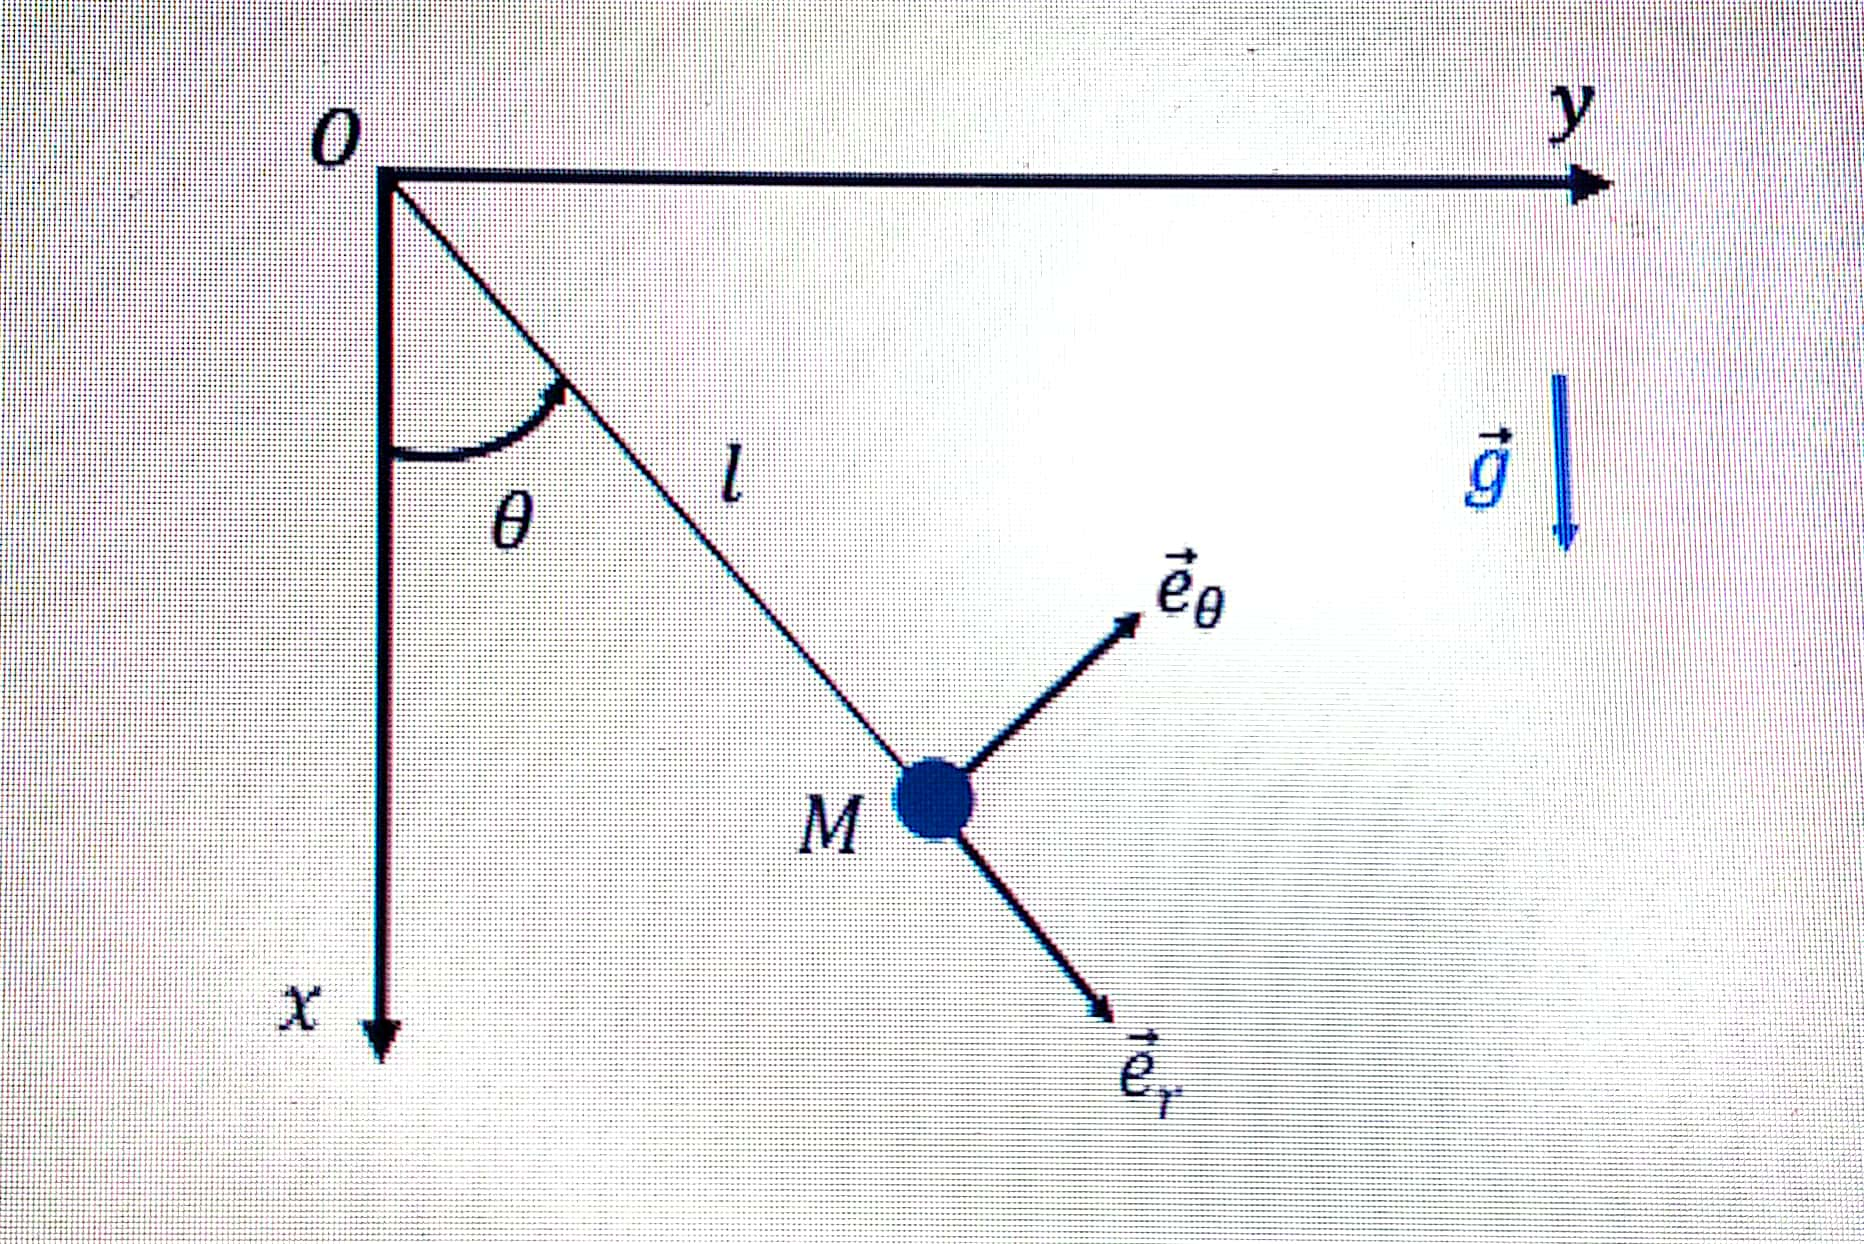
\includegraphics[width=0.55\textwidth]{images/mpm/mpm-012-001.png}
\captionof{figure}{\small Bilan énergétique avant/après choc : l'énergie cinétique est intégralement transférée entre les deux billes.}
\end{center}
\end{boitecorrige}

\subsection*{Exercice 10 - Satellite géostationnaire et troisième loi de Kepler \niveau{\moyen}}

\newpage
\begin{boiteexercice}
Un satellite géostationnaire orbite au-dessus de l'équateur à l'altitude $h = \qty{35800}{km}$.
\begin{enumerate}
  \item Calculer le rayon orbital $r = R_T + h$ avec $R_T = \qty{6371}{km}$.
  \item Calculer la vitesse orbitale $v = \sqrt{GM/r}$ avec $GM = \qty{3.98e14}{m^3.s^{-2}}$.
  \item Calculer la période $T = 2\pi r / v$ et vérifier qu'elle vaut environ $\qty{86400}{s} = \qty{24}{h}$.
  \item Vérifier la troisième loi de Kepler pour ce satellite et le satellite à $h = \qty{400}{km}$ (Exercice 4, $T \approx \qty{5573}{s}$).
\end{enumerate}
\end{boiteexercice}

\begin{boitecorrige}
\textbf{1.} Rayon orbital :
\[
r = R_T + h = (6371 + 35800)\times10^3 = 42171\times10^3 \approx \qty{4.217e7}{m}
\]

\textbf{2.} Vitesse orbitale :
\[
v = \sqrt{\frac{GM}{r}} = \sqrt{\frac{3{,}98\times10^{14}}{4{,}217\times10^7}} = \sqrt{9{,}437\times10^6} \approx \qty{3072}{m.s^{-1}}
\]

\textbf{3.} Période de révolution :
\[
T = \frac{2\pi r}{v} = \frac{2\pi\times4{,}217\times10^7}{3072} \approx \frac{2{,}649\times10^8}{3072} \approx \qty{86232}{s} \approx \qty{23.95}{h}
\]
Ce résultat est très proche de $\qty{86400}{s} = \qty{24}{h}$, ce qui justifie le caractère géostationnaire de cet orbite.
\end{boitecorrige}

\begin{center}

\includegraphics[width=0.85\textwidth]{images/mpm/mpm-014-002.png}
\captionof{figure}{\small Orbite géostationnaire : le satellite survole toujours le même point de l'équateur terrestre.}
\end{center}

\begin{boitecorrige}
\textbf{4.} La troisième loi de Kepler prédit $T^2/r^3 = 4\pi^2/(GM) = \text{cste}$.

Pour l'ISS ($r_1 = 6{,}8\times10^6\,\text{m}$, $T_1 = 5573\,\text{s}$) :
\[
\frac{T_1^2}{r_1^3} = \frac{(5573)^2}{(6{,}8\times10^6)^3} = \frac{3{,}106\times10^7}{3{,}144\times10^{20}} \approx 9{,}88\times10^{-14}
\]
Pour le satellite géostationnaire ($r_2 \approx 4{,}217\times10^7\,\text{m}$, $T_2 \approx 86232\,\text{s}$) :
\[
\frac{T_2^2}{r_2^3} = \frac{(86232)^2}{(4{,}217\times10^7)^3} = \frac{7{,}436\times10^9}{7{,}502\times10^{22}} \approx 9{,}91\times10^{-14}
\]
Les deux valeurs sont bien égales : la troisième loi est vérifiée.
\end{boitecorrige}

\begin{center}
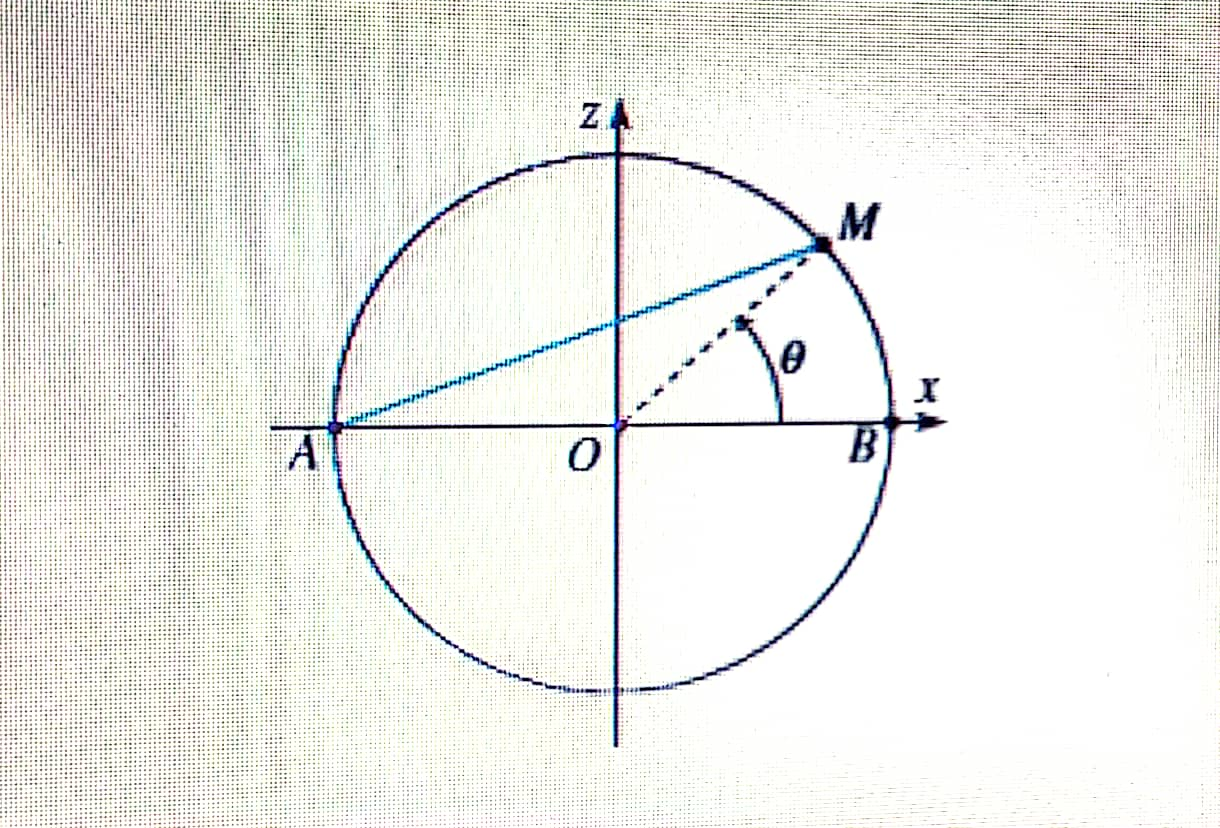
\includegraphics[width=0.55\textwidth]{images/mpm/mpm-014-003.png}
\captionof{figure}{\small Vérification graphique de la troisième loi de Kepler : $T^2$ en fonction de $r^3$ est une droite passant par l'origine.}
\end{center}

\subsection*{Exercice 11 - Théorème travail-énergie \niveau{\moyen}}

\begin{boiteexercice}
Un bloc de masse $m = \qty{10}{kg}$ est initialement au repos sur une surface horizontale. Une force horizontale $F = \qty{80}{N}$ lui est appliquée sur une distance $d = \qty{5}{m}$. Le coefficient de frottement cinétique entre le bloc et la surface est $\mu_k = 0{,}25$.
\begin{enumerate}
  \item Calculer le travail $W_F$ de la force $F$.
  \item Calculer le travail $W_{frot}$ des forces de frottement.
  \item Appliquer le théorème travail-énergie pour calculer la variation d'énergie cinétique $\Delta E_c = W_F + W_{frot}$.
  \item En déduire la vitesse finale $v_f$.
\end{enumerate}
\textbf{Donnée :} $g = \qty{9.81}{m.s^{-2}}$.
\end{boiteexercice}

\begin{boitecorrige}
\textbf{1.} Travail de la force $F$ :
\[
W_F = F\cdot d = 80\times5 = \qty{400}{J}
\]

\textbf{2.} La réaction normale est $N = mg = 10\times9{,}81 = \qty{98.1}{N}$.

La force de frottement cinétique est $f_k = \mu_k N = 0{,}25\times98{,}1 = \qty{24.525}{N}$.

Son travail (force opposée au déplacement) :
\[
W_{frot} = -f_k\cdot d = -24{,}525\times5 = \qty{-122.6}{J}
\]

\textbf{3.} Par le théorème travail-énergie :
\[
\Delta E_c = W_{total} = W_F + W_{frot} = 400 + (-122{,}6) = \qty{277.4}{J}
\]

\textbf{4.} Avec $v_0 = 0$, $E_{c,i} = 0$ :
\[
\frac{1}{2}mv_f^2 = \Delta E_c = \qty{277.4}{J}
\]
\[
v_f = \sqrt{\frac{2\times277{,}4}{10}} = \sqrt{55{,}48} \approx \qty{7.45}{m.s^{-1}}
\]
\end{boitecorrige}

\subsection*{Exercice 12 - Oscillateur harmonique amorti \niveau{\difficile}}

\newpage
\begin{boiteexercice}
Un oscillateur harmonique amorti obéit à l'équation :
\[
m\ddot{x} + b\dot{x} + kx = 0
\]
avec $m = \qty{1}{kg}$, $k = \qty{100}{N.m^{-1}}$, $b = \qty{4}{N.s.m^{-1}}$.
\begin{enumerate}
  \item Calculer la pulsation propre $\omega_0 = \sqrt{k/m}$ et le facteur de qualité $Q = m\omega_0/b$.
  \item Déterminer le régime d'amortissement (sous-amorti, critique ou sur-amorti) en comparant $b$ à $b_c = 2\sqrt{km}$.
  \item Donner la solution générale $x(t) = A\,e^{-bt/(2m)}\cos(\omega t + \varphi)$ et calculer $\omega = \sqrt{\omega_0^2 - (b/2m)^2}$.
  \item Avec les conditions initiales $x(0) = \qty{0.1}{m}$ et $\dot{x}(0) = 0$, déterminer $A$ et $\varphi$.
\end{enumerate}
\end{boiteexercice}

\begin{boitecorrige}
\textbf{1.} Pulsation propre et facteur de qualité :
\[
\omega_0 = \sqrt{\frac{k}{m}} = \sqrt{\frac{100}{1}} = \qty{10}{rad.s^{-1}}
\]
\[
Q = \frac{m\omega_0}{b} = \frac{1\times10}{4} = 2{,}5
\]

\textbf{2.} L'amortissement critique correspond à $b_c = 2\sqrt{km} = 2\sqrt{100\times1} = \qty{20}{N.s.m^{-1}}$.

Ici $b = \qty{4}{N.s.m^{-1}} < b_c = \qty{20}{N.s.m^{-1}}$, donc on est en régime \textbf{sous-amorti} ($Q > 1/2$).

\textbf{3.} En régime sous-amorti, la solution est :
\[
x(t) = A\,e^{-bt/(2m)}\cos(\omega t + \varphi)
\]
avec
\[
\omega = \sqrt{\omega_0^2 - \left(\frac{b}{2m}\right)^2} = \sqrt{100 - \left(\frac{4}{2}\right)^2} = \sqrt{100 - 4} = \sqrt{96} \approx \qty{9.80}{rad.s^{-1}}
\]
Le coefficient d'amortissement est $\gamma = b/(2m) = 4/(2\times1) = \qty{2}{s^{-1}}$.
\end{boitecorrige}

\begin{center}

\includegraphics[width=0.85\textwidth]{images/mpm/mpm-015-004.png}
\captionof{figure}{\small Régime sous-amorti : oscillations de pulsation $\omega$ amorties exponentiellement par $e^{-\gamma t}$.}
\end{center}

\clearpage
\begin{boitecorrige}
\textbf{4.} Conditions initiales $x(0) = 0{,}1\,\text{m}$ et $\dot{x}(0) = 0$ :
\[
x(0) = A\cos\varphi = 0{,}1
\]
\[
\dot{x}(0) = A\left(-\gamma\cos\varphi - \omega\sin\varphi\right) = 0 \quad \Rightarrow \quad \tan\varphi = -\frac{\gamma}{\omega} = -\frac{2}{9{,}80} \approx -0{,}204
\]
\[
\varphi = \arctan(-0{,}204) \approx -0{,}202\,\text{rad}, \qquad A = \frac{0{,}1}{\cos\varphi} \approx \frac{0{,}1}{0{,}979} \approx \qty{0.102}{m}
\]
La solution est donc : $x(t) \approx 0{,}102\,e^{-2t}\cos(9{,}80\,t - 0{,}202)\,[\text{m}]$.
\end{boitecorrige}

\begin{center}
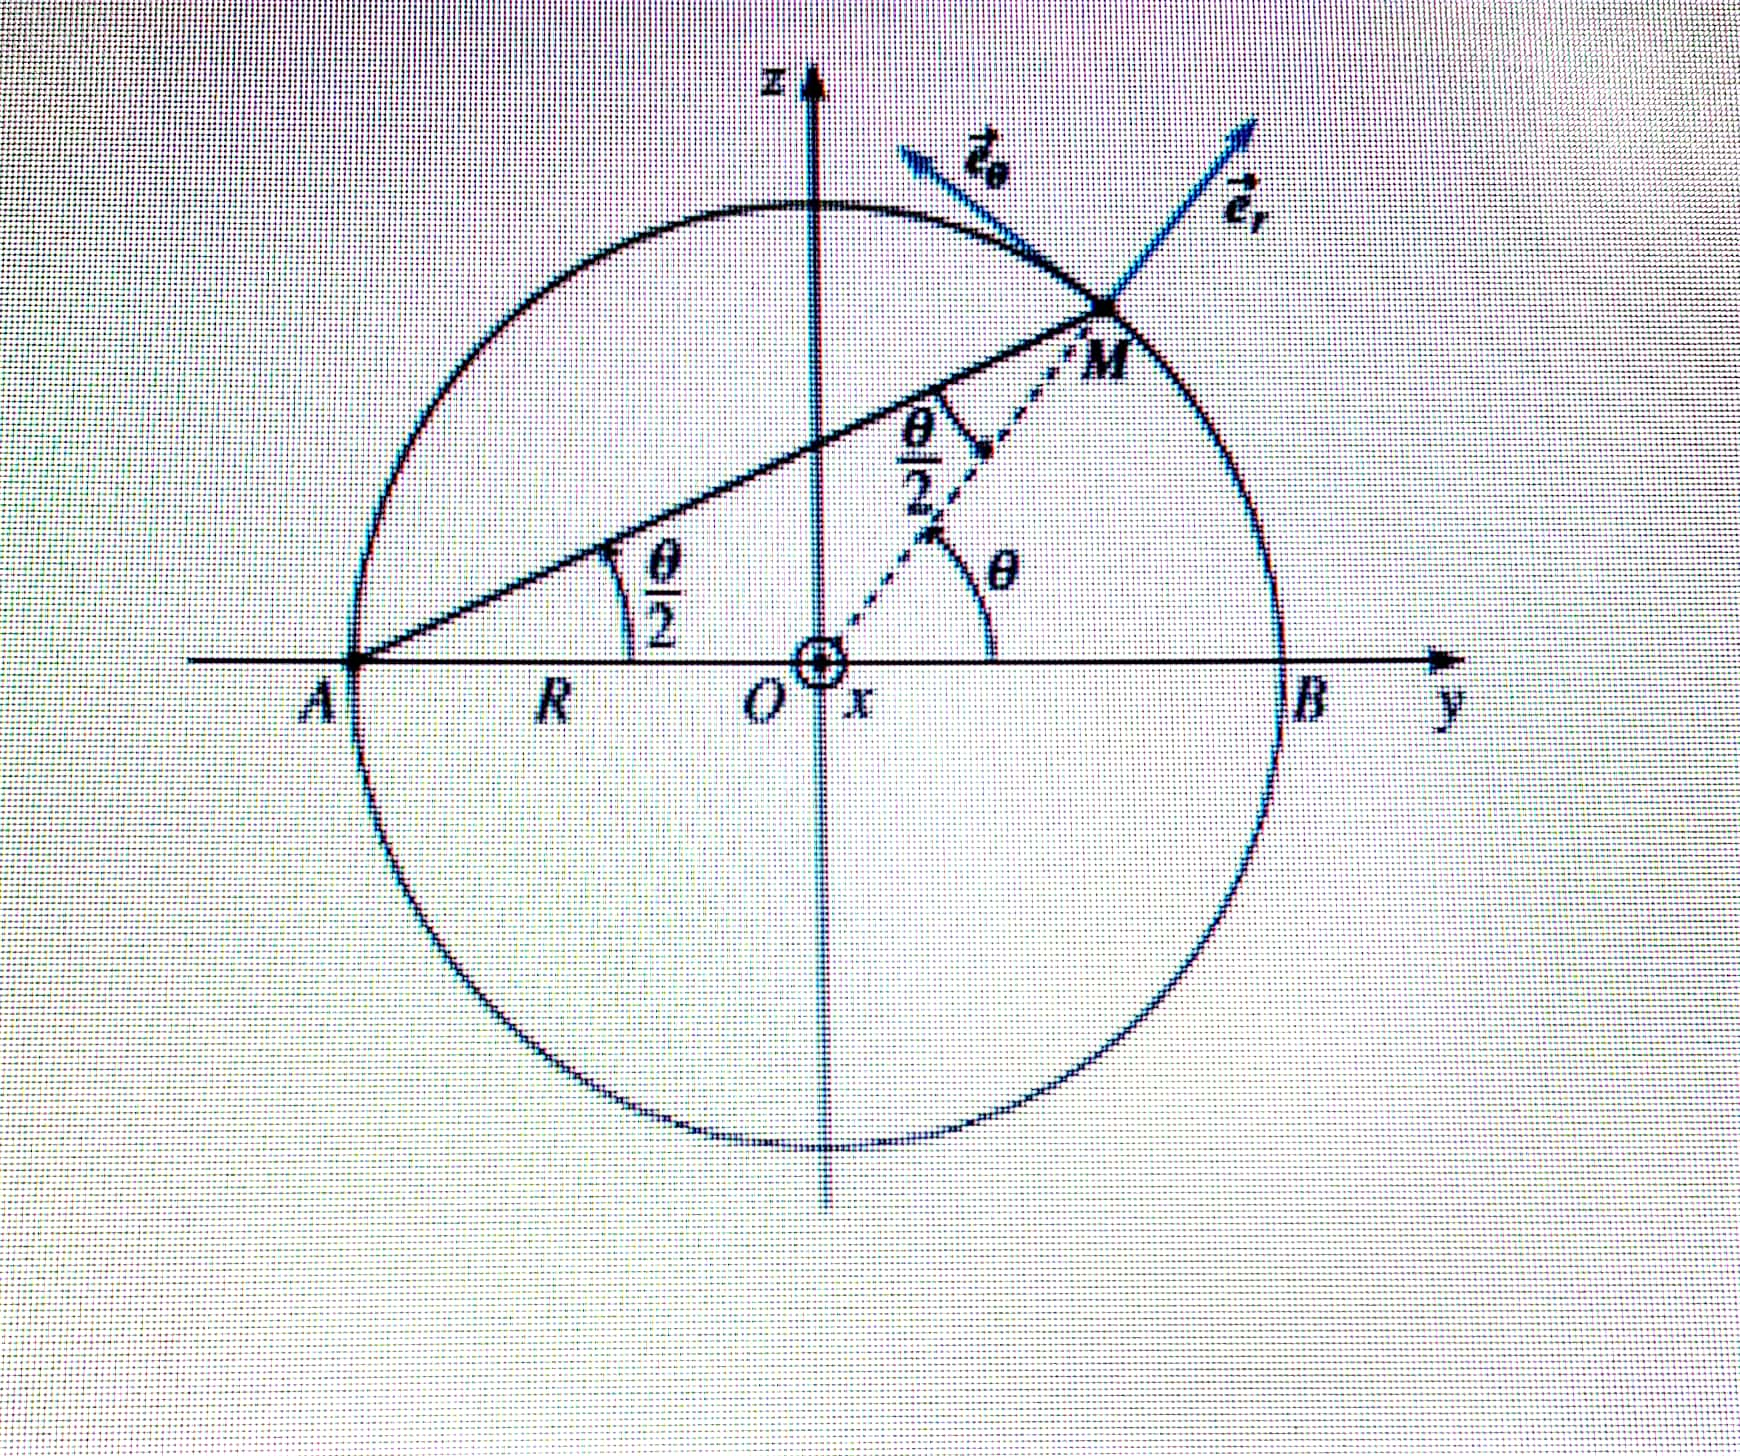
\includegraphics[width=0.55\textwidth]{images/mpm/mpm-015-005.png}
\captionof{figure}{\small Détermination graphique de $A$ et $\varphi$ à partir des conditions initiales.}
\end{center}

\subsection*{Exercice 13 - Chute verticale avec résistance de l'air \niveau{\difficile}}

\begin{boiteexercice}
Un parachutiste de masse totale $m = \qty{80}{kg}$ tombe en chute libre. La force de résistance de l'air est $f = -bv$ avec $b = \qty{10}{kg.s^{-1}}$. Il commence avec une vitesse nulle ($v(0)=0$).
\begin{enumerate}
  \item Écrire l'équation différentielle du mouvement (axe $z$ orienté vers le bas) :
  $m\dot{v} = mg - bv$.
  \item Résoudre cette équation et trouver $v(t)$.
  \item Déterminer la vitesse limite $v_\infty = mg/b$ et calculer sa valeur numérique.
  \item Calculer le temps $t^* = m/b$ au bout duquel le parachutiste atteint $63\,\%$ de la vitesse limite.
  \item Déterminer $z(t)$ (position), en prenant $z(0) = 0$.
\end{enumerate}
\textbf{Donnée :} $g = \qty{9.81}{m.s^{-2}}$.
\end{boiteexercice}

\begin{boitecorrige}
\textbf{1.} Bilan des forces sur l'axe vertical descendant : poids $mg$ (vers le bas) et frottement $-bv$ (vers le haut si $v > 0$) :
\[
m\dot{v} = mg - bv
\]

\textbf{2.} L'équation s'écrit $\dot{v} + \frac{b}{m}v = g$. En posant $\alpha = b/m$ :
\[
\frac{\d v}{g - \alpha v} = \d t \quad \Rightarrow \quad -\frac{1}{\alpha}\ln|g - \alpha v| = t + C
\]
Avec $v(0) = 0$ : $C = -\frac{1}{\alpha}\ln g$.
\[
v(t) = \frac{g}{\alpha}\left(1 - \e^{-\alpha t}\right) = \frac{mg}{b}\left(1 - \e^{-bt/m}\right)
\]

\textbf{3.} Vitesse limite ($t \to \infty$) :
\[
v_\infty = \frac{mg}{b} = \frac{80\times9{,}81}{10} = \qty{78.5}{m.s^{-1}} \approx \qty{283}{km.h^{-1}}
\]

\textbf{4.} Temps caractéristique :
\[
t^* = \frac{m}{b} = \frac{80}{10} = \qty{8}{s}
\]
À $t = t^*$ : $v(t^*) = v_\infty(1 - \e^{-1}) \approx 0{,}632\,v_\infty = \qty{49.6}{m.s^{-1}}$.

\textbf{5.} En intégrant $v(t)$ :
\begin{align*}
z(t) &= \int_0^t v(t')\,\d t' = v_\infty\int_0^t \left(1-\e^{-t'/t^*}\right)\d t' \\
&= v_\infty\left[t + t^*\e^{-t/t^*}\right]_0^t = v_\infty\left(t + t^*\e^{-t/t^*} - t^*\right) \\
&= v_\infty\left(t - t^*\left(1 - \e^{-t/t^*}\right)\right)
\end{align*}
Soit numériquement : $z(t) = 78{,}5\left(t - 8(1-\e^{-t/8})\right)$ [m].
\end{boitecorrige}

\subsection*{Exercice 14 - Conservation de l'énergie : ressort et gravité \niveau{\moyen}}

\begin{boiteexercice}
Une masse $m = \qty{2}{kg}$ est attachée à un ressort vertical de constante de raideur $k = \qty{50}{N.m^{-1}}$ et de longueur à vide $L_0$. Le système est en position d'équilibre. On écarte la masse d'une distance $A = \qty{5}{cm}$ vers le bas et on la lâche.
\begin{enumerate}
  \item Calculer l'allongement à l'équilibre $\delta = mg/k$.
  \item En prenant comme référence de l'énergie potentielle gravitationnelle le point d'équilibre, écrire l'énergie mécanique totale $E_m = \frac{1}{2}mv^2 + \frac{1}{2}k x^2$ (où $x$ est l'écart à l'équilibre). Justifier.
  \item Calculer la vitesse maximale $v_{max}$ atteinte en $x = 0$.
  \item Calculer la pulsation des oscillations $\omega_0 = \sqrt{k/m}$ et la période $T$.
  \item À quelle position $x_1$ la vitesse vaut-elle $v_{max}/\sqrt{2}$ ?
\end{enumerate}
\textbf{Données :} $g = \qty{9.81}{m.s^{-2}}$.
\end{boiteexercice}

\begin{boitecorrige}
\textbf{1.} À l'équilibre, le ressort est allongé de :
\[
\delta = \frac{mg}{k} = \frac{2\times9{,}81}{50} = \qty{0.392}{m} \approx \qty{39.2}{cm}
\]

\textbf{2.} En notant $x$ l'écart par rapport à la position d'équilibre (positif vers le bas), les forces sur la masse sont : $mg$ (bas) et $-k(\delta+x)$ (ressort, haut). Le bilan :
\[
m\ddot{x} = mg - k(\delta+x) = mg - k\delta - kx = -kx
\]
(car $mg = k\delta$ à l'équilibre). L'énergie potentielle effective (gravité + ressort, au 2e ordre en $x$) se réduit à $\frac{1}{2}kx^2$ autour de l'équilibre. L'énergie mécanique est :
\[
E_m = \frac{1}{2}mv^2 + \frac{1}{2}kx^2 = \text{constante}
\]

\textbf{3.} À $t=0$ : $x = A = \qty{0.05}{m}$, $v = 0$, donc $E_m = \frac{1}{2}kA^2$.
En $x = 0$ : $\frac{1}{2}mv_{max}^2 = \frac{1}{2}kA^2$.
\[
v_{max} = A\sqrt{\frac{k}{m}} = 0{,}05\times\sqrt{\frac{50}{2}} = 0{,}05\times5 = \qty{0.25}{m.s^{-1}}
\]

\textbf{4.} Pulsation et période :
\[
\omega_0 = \sqrt{\frac{k}{m}} = \sqrt{\frac{50}{2}} = \qty{5}{rad.s^{-1}}, \quad T = \frac{2\pi}{\omega_0} = \frac{2\pi}{5} \approx \qty{1.26}{s}
\]

\textbf{5.} On cherche $x_1$ tel que $v = v_{max}/\sqrt{2}$ :
\[
\frac{1}{2}m\frac{v_{max}^2}{2} + \frac{1}{2}kx_1^2 = \frac{1}{2}kA^2
\]
\[
\frac{1}{2}kx_1^2 = \frac{1}{2}kA^2 - \frac{1}{4}kA^2 = \frac{1}{4}kA^2 \quad \Rightarrow \quad x_1 = \frac{A}{\sqrt{2}} = \frac{0{,}05}{\sqrt{2}} \approx \qty{3.54}{cm}
\]
\end{boitecorrige}

\subsection*{Exercice 15 - Mouvement dans un champ gravitationnel : orbite elliptique \niveau{\difficile}}

\begin{boiteexercice}
On considère un satellite de masse $m$ en orbite circulaire autour de la Terre (masse $M_T$, rayon $R_T = \qty{6371}{km}$).
\begin{enumerate}
  \item À l'altitude $h = \qty{400}{km}$ (altitude de la Station Spatiale Internationale), calculer le rayon orbital $r = R_T + h$, la vitesse orbitale $v = \sqrt{GM_T/r}$ et la période $T$.
  \item Montrer que l'énergie mécanique totale du satellite est $E = -\frac{GM_T m}{2r}$ (état lié).
  \item Calculer la vitesse de libération depuis la surface terrestre : $v_L = \sqrt{2GM_T/R_T}$.
  \item La troisième loi de Kepler : $T^2 = \frac{4\pi^2}{GM_T}\,r^3$. Vérifier avec les valeurs ci-dessus.
\end{enumerate}
\textbf{Données :} $G = \qty{6.674e-11}{N.m^2.kg^{-2}}$, $M_T = \qty{5.972e24}{kg}$, $g_0 = \qty{9.81}{m.s^{-2}}$.
\end{boiteexercice}

\begin{boitecorrige}
\textbf{1.} Rayon orbital :
\[
r = R_T + h = 6371 + 400 = \qty{6771}{km} = \qty{6.771e6}{m}
\]
Pour une orbite circulaire, la force de gravitation fournit la force centripète :
\[
\frac{GM_T m}{r^2} = \frac{mv^2}{r} \quad \Rightarrow \quad v = \sqrt{\frac{GM_T}{r}}
\]
\[
v = \sqrt{\frac{6{,}674\times10^{-11}\times5{,}972\times10^{24}}{6{,}771\times10^6}}
= \sqrt{\frac{3{,}986\times10^{14}}{6{,}771\times10^6}} = \sqrt{5{,}887\times10^7} \approx \qty{7673}{m.s^{-1}}
\]
\[
T = \frac{2\pi r}{v} = \frac{2\pi\times6{,}771\times10^6}{7673} \approx \qty{5545}{s} \approx \qty{92.4}{min}
\]

\textbf{2.} Énergie cinétique : $E_c = \frac{1}{2}mv^2 = \frac{GM_T m}{2r}$.

Énergie potentielle gravitationnelle : $E_p = -\frac{GM_T m}{r}$.

Énergie totale :
\[
E = E_c + E_p = \frac{GM_T m}{2r} - \frac{GM_T m}{r} = -\frac{GM_T m}{2r} < 0
\]
L'énergie négative confirme que le satellite est lié (orbite fermée).

\textbf{3.} Vitesse de libération (énergie totale nulle depuis la surface) :
\[
E = \frac{1}{2}mv_L^2 - \frac{GM_T m}{R_T} = 0 \quad \Rightarrow \quad v_L = \sqrt{\frac{2GM_T}{R_T}}
\]
\[
v_L = \sqrt{\frac{2\times6{,}674\times10^{-11}\times5{,}972\times10^{24}}{6{,}371\times10^6}}
= \sqrt{1{,}252\times10^8} \approx \qty{11.19}{km.s^{-1}}
\]

\textbf{4.} Vérification de la 3e loi de Kepler :
\[
T^2 = \frac{4\pi^2}{GM_T}r^3 = \frac{4\pi^2}{3{,}986\times10^{14}}\times(6{,}771\times10^6)^3
\]
\[
= \frac{39{,}48}{3{,}986\times10^{14}}\times3{,}103\times10^{20} = \frac{39{,}48\times3{,}103\times10^{20}}{3{,}986\times10^{14}} \approx 3{,}073\times10^7
\]
\[
T = \sqrt{3{,}073\times10^7} \approx \qty{5543}{s}
\]
Résultat en accord avec le calcul direct : $T \approx \qty{5545}{s}$.

\begin{center}

\includegraphics[width=0.7\textwidth]{images/mpm/mpm-027-006.png}
\captionof{figure}{\small Orbite circulaire autour de la Terre : équilibre entre attraction gravitationnelle et force centripète.}
\end{center}
\begin{center}
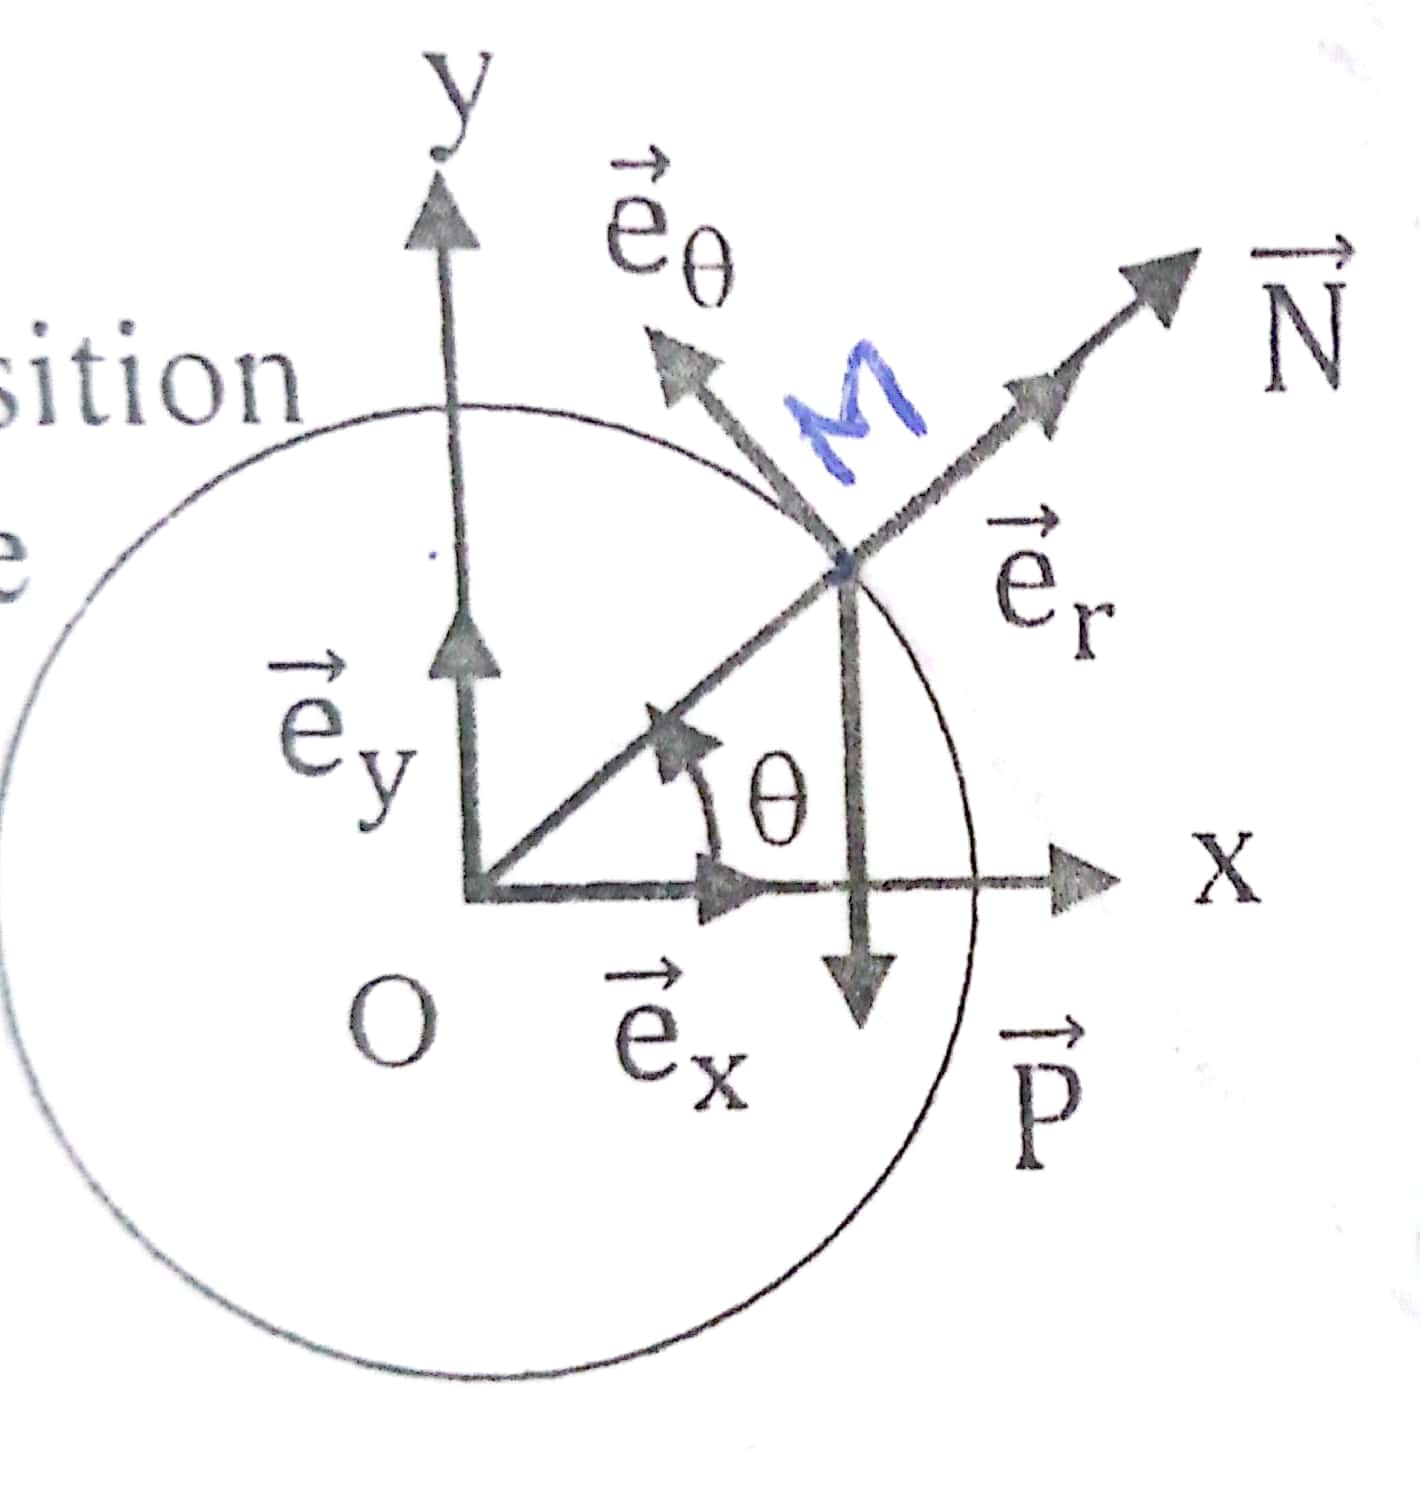
\includegraphics[width=0.55\textwidth]{images/mpm/mpm-027-007.png}
\captionof{figure}{\small Vitesse de libération et orbite de libération : $v_L = \sqrt{2GM_T/R_T}$.}
\end{center}
\end{boitecorrige}


\subsection*{Exercice 16 - Projectile avec frottement visqueux (2D) \niveau{\moyen}}

\begin{boiteexercice}
Un projectile de masse $m$ est lancé avec une vitesse initiale $v_0$ à un angle $\theta$ par rapport à l'horizontale. L'air exerce un frottement visqueux $\vec{f} = -k\vec{v}$ ($k > 0$).

\begin{enumerate}
  \item Écrire les équations du mouvement (PFD) selon les axes $x$ (horizontal) et $y$ (vertical, positif vers le haut) :
  \[
  m\dot{v}_x = -kv_x, \qquad m\dot{v}_y = -mg - kv_y
  \]
  \item Résoudre ces deux équations différentielles avec les conditions initiales $v_x(0) = v_0\cos\theta$ et $v_y(0) = v_0\sin\theta$. Montrer que :
  \[
  v_x(t) = v_0\cos\theta\,\e^{-kt/m}, \qquad v_y(t) = \left(v_0\sin\theta + \frac{mg}{k}\right)\e^{-kt/m} - \frac{mg}{k}
  \]
  \item En intégrant les vitesses, donner les expressions de $x(t)$ et $y(t)$ avec $x(0) = y(0) = 0$.
  \item Comparer qualitativement la portée avec et sans frottement. Dans quel sens le frottement modifie-t-il la trajectoire ?
\end{enumerate}

\textbf{Application numérique :} $m = \qty{0.5}{kg}$, $v_0 = \qty{30}{m.s^{-1}}$, $\theta = 45^\circ $, $k = \qty{0.05}{kg.s^{-1}}$, $g = \qty{9.81}{m.s^{-2}}$.
\end{boiteexercice}

\begin{boitecorrige}
\textbf{1.} En appliquant le PFD selon chaque axe, avec $\vec{f} = -k\vec{v}$ :
\[
m\ddot{x} = -k\dot{x} = -kv_x \qquad m\ddot{y} = -mg - kv_y
\]

\textbf{2. Résolution des EDO.}

\textit{Composante $x$ :} L'équation $m\dot{v}_x = -kv_x$ est homogène. On pose $\alpha = k/m$ :
\[
\dot{v}_x + \alpha v_x = 0 \quad \Rightarrow \quad v_x(t) = C_1\,\e^{-\alpha t}
\]
Avec $v_x(0) = v_0\cos\theta$ :
\[
\boxed{v_x(t) = v_0\cos\theta\,\e^{-kt/m}}
\]

\textit{Composante $y$ :} L'équation $m\dot{v}_y = -mg - kv_y$ s'écrit $\dot{v}_y + \alpha v_y = -g$. Solution particulière : $v_{y,p} = -g/\alpha = -mg/k$. Solution générale :
\[
v_y(t) = C_2\,\e^{-\alpha t} - \frac{mg}{k}
\]
Avec $v_y(0) = v_0\sin\theta$ :
\[
C_2 = v_0\sin\theta + \frac{mg}{k}
\]
\[
\boxed{v_y(t) = \left(v_0\sin\theta + \frac{mg}{k}\right)\e^{-kt/m} - \frac{mg}{k}}
\]

\textbf{3. Positions par intégration.}

\[
x(t) = \int_0^t v_x\,\d t' = \frac{mv_0\cos\theta}{k}\left(1 - \e^{-kt/m}\right)
\]

\[
y(t) = \int_0^t v_y\,\d t' = \frac{m}{k}\left(v_0\sin\theta + \frac{mg}{k}\right)\left(1 - \e^{-kt/m}\right) - \frac{mg}{k}\,t
\]

En développant et regroupant :
\[
\boxed{x(t) = \frac{mv_0\cos\theta}{k}\left(1 - \e^{-kt/m}\right)}
\]
\[
\boxed{y(t) = \left(\frac{mv_0\sin\theta}{k} + \frac{m^2 g}{k^2}\right)\left(1 - \e^{-kt/m}\right) - \frac{mg}{k}\,t}
\]

\textbf{4. Comparaison avec et sans frottement.}

Sans frottement ($k = 0$, vérifiable par développement en série de Taylor à l'ordre 1 en $k$), on retrouve les équations classiques $x = v_0\cos\theta\cdot t$, $y = v_0\sin\theta\cdot t - \frac{1}{2}gt^2$.

Avec frottement :
\begin{itemize}[nosep]
  \item La composante horizontale décélère exponentiellement : $x \to mv_0\cos\theta/k$ (limite finie), alors que sans frottement $x$ croît indéfiniment.
  \item La composante verticale tend vers la vitesse limite $-mg/k$ (chute terminale).
  \item La portée est donc \textbf{réduite} par le frottement.
  \item La trajectoire n'est plus symétrique : la descente est plus raide que la montée.
\end{itemize}

\textbf{Application numérique.}

$\alpha = k/m = 0{,}05/0{,}5 = \qty{0.1}{s^{-1}}$, $mg/k = 0{,}5\times9{,}81/0{,}05 = \qty{98.1}{m.s^{-1}}$.

Sans frottement : portée $R_0 = v_0^2\sin(2\theta)/g = 900/9{,}81 \approx \qty{91.7}{m}$.

Avec frottement, la portée est plus faible (le projectile touche le sol avant $x = \qty{91.7}{m}$).

\begin{center}

\includegraphics[width=0.7\textwidth]{images/mpm/mpm-028-008.png}
\captionof{figure}{\small Trajectoire d'un projectile avec frottement visqueux : la portée est réduite par rapport au cas sans frottement.}
\end{center}
\begin{center}
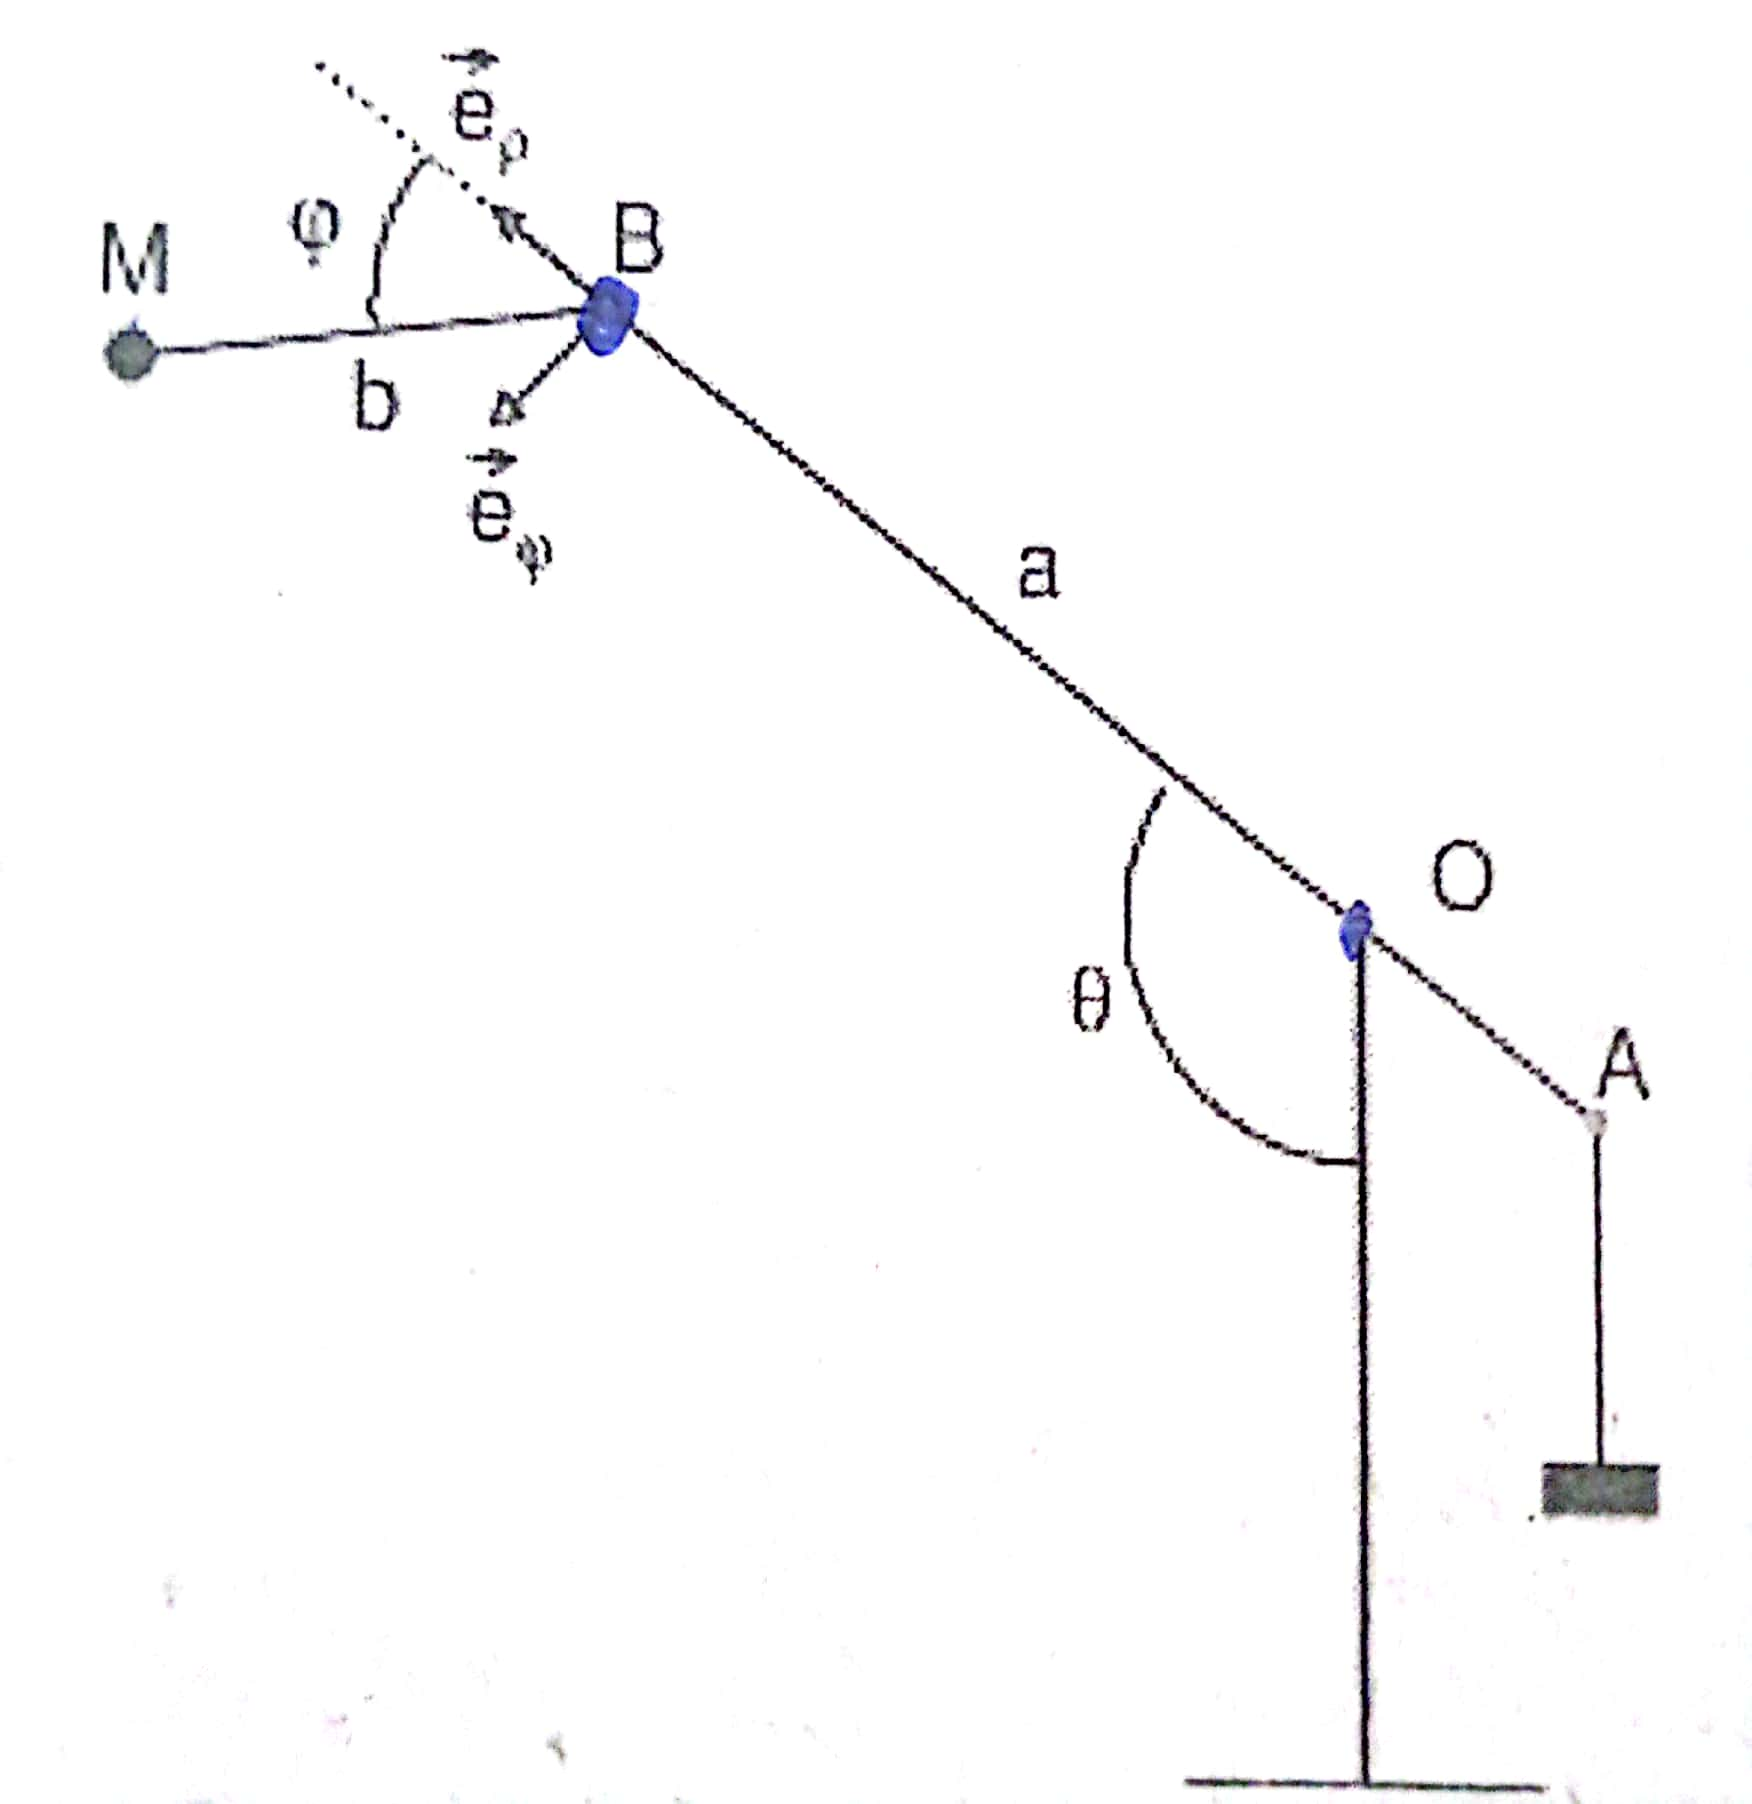
\includegraphics[width=0.55\textwidth]{images/mpm/mpm-028-009.png}
\captionof{figure}{\small Comparaison des vitesses $v_x(t)$ et $v_y(t)$ en présence de frottement fluide.}
\end{center}
\end{boitecorrige}

\subsection*{Exercice 17 - Énergie mécanique du pendule simple \niveau{\moyen}}

\begin{boiteexercice}
Un pendule simple est constitué d'une masse $m = \qty{0.2}{kg}$ suspendue à un fil de longueur $L = \qty{0.8}{m}$. On désigne par $\theta$ l'angle que fait le fil avec la verticale. Le pendule est lâché depuis $\theta_0 = 30^\circ $ sans vitesse initiale.

\begin{center}
\begin{tikzpicture}[scale=1.1]
  % Support
  \fill[gray!50] (-0.15,0) rectangle (0.15,0.15);
  \draw[gray!60, thick] (-0.9,0.15) -- (0.9,0.15);
  \fill (0,0) circle (0.055);
  % Verticale
  \draw[gray!35, dashed] (0,0) -- (0,-2.2);
  % Fil à theta0=30°
  \draw[thick] (0,0) -- ({sin(30)*1.8}, {-cos(30)*1.8});
  \shade[ball color=blue!55] ({sin(30)*1.8}, {-cos(30)*1.8}) circle (0.17);
  % Angle theta0
  \draw[->, blue!60] (0,-0.6) arc(-90:{-90+30}:0.6);
  \node[blue!70, font=\small] at (0.28, -0.52) {$\theta_0$};
  % L
  \node[left, font=\small] at (-0.12, -0.85) {$L$};
  % Position equilibre (bas)
  \shade[ball color=gray!30] (0,-1.8) circle (0.17);
  \draw[dashed, gray!50] (0,0) -- (0,-1.8);
  % Hauteur hmax
  \draw[<->, red!70] ({sin(30)*1.8+0.25}, {-cos(30)*1.8}) -- (0.25,-1.8);
  \node[red!70, right, font=\small] at (0.3, {(-cos(30)*1.8-1.8)/2}) {$h_{max}$};
  % Energie cinetique max en bas (flèche)
  \draw[->, green!60!black, very thick] (-0.25,-1.8) -- (-0.25,-1.2)
    node[left, font=\scriptsize] {$v_{max}$};
\end{tikzpicture}
\captionof{figure}{\small Pendule lâché de $\theta_0=30°$. L'énergie potentielle $E_p = mgL(1-\cos\theta_0)$ se convertit en énergie cinétique $\frac{1}{2}mv_{max}^2$ au passage par la verticale.}
\end{center}

\begin{enumerate}
  \item Écrire l'équation du mouvement (sans approximation des petits angles) :
  \[
  mL^2\ddot{\theta} = -mgL\sin\theta
  \]
  \item En utilisant la conservation de l'énergie mécanique, écrire :
  \[
  E_m = \frac{1}{2}mL^2\dot{\theta}^2 + mgL(1-\cos\theta) = \text{cste}
  \]
  Calculer la valeur de $E_m$ pour les conditions initiales données.
  \item En déduire la vitesse angulaire $\dot{\theta}$ en fonction de $\theta$. Calculer $\dot{\theta}$ quand $\theta = 0$ (passage par la verticale).
  \item En déduire la vitesse linéaire $v = L\dot{\theta}$ de la masse en bas de sa trajectoire.
  \item Linéariser l'équation du mouvement pour les petits angles. Calculer la période $T = 2\pi\sqrt{L/g}$ pour ce pendule.
  \item Quelle est la hauteur maximale $h_{max}$ atteinte par la masse au-dessus de sa position basse ?
\end{enumerate}
\textbf{Donnée :} $g = \qty{9.81}{m.s^{-2}}$.
\end{boiteexercice}

\begin{boitecorrige}
\textbf{1. Équation du mouvement.}

En appliquant le théorème du moment cinétique par rapport au point d'accrochage, avec le moment du poids :
\[
mL^2\ddot{\theta} = -mgL\sin\theta \quad \Rightarrow \quad \ddot{\theta} + \frac{g}{L}\sin\theta = 0
\]
C'est un oscillateur non linéaire.

\textbf{2. Énergie mécanique.}

L'énergie cinétique est $E_c = \frac{1}{2}mv^2 = \frac{1}{2}m(L\dot\theta)^2 = \frac{1}{2}mL^2\dot\theta^2$.

L'énergie potentielle gravitationnelle (avec origine en bas de la trajectoire, où $\theta = 0$) est :
$E_p = mgh = mgL(1 - \cos\theta)$ (la masse est à la hauteur $L - L\cos\theta = L(1-\cos\theta)$ au-dessus du point le plus bas).

\[
E_m = \frac{1}{2}mL^2\dot{\theta}^2 + mgL(1-\cos\theta)
\]

À $t = 0$ : $\theta = \theta_0 = 30^\circ $, $\dot{\theta} = 0$ :
\[
E_m = 0 + mgL(1-\cos 30^\circ ) = 0{,}2\times9{,}81\times0{,}8\times(1 - \frac{\sqrt{3}}{2})
\]
\[
E_m = 1{,}5696\times(1 - 0{,}866) = 1{,}5696\times0{,}134 \approx \qty{0.210}{J}
\]

\textbf{3. Vitesse angulaire en fonction de $\theta$.}

Par conservation de l'énergie :
\[
\frac{1}{2}mL^2\dot\theta^2 = E_m - mgL(1-\cos\theta) = mgL(\cos\theta - \cos\theta_0)
\]
\[
\boxed{\dot\theta = \pm\sqrt{\frac{2g}{L}(\cos\theta - \cos\theta_0)}}
\]

En $\theta = 0$ (verticale) :
\[
\dot\theta_{max} = \sqrt{\frac{2g}{L}(1 - \cos\theta_0)} = \sqrt{\frac{2\times9{,}81}{0{,}8}(1-\cos 30^\circ )} = \sqrt{24{,}525\times0{,}134} \approx \qty{1.814}{rad.s^{-1}}
\]

\textbf{4. Vitesse linéaire en bas.}
\[
v_{max} = L\,\dot\theta_{max} = 0{,}8\times1{,}814 \approx \qty{1.45}{m.s^{-1}}
\]

On peut aussi retrouver ce résultat par la conservation de l'énergie : $\frac{1}{2}mv_{max}^2 = E_m$, soit $v_{max} = \sqrt{2E_m/m} = \sqrt{2\times0{,}210/0{,}2} = \sqrt{2{,}1} \approx \qty{1.449}{m.s^{-1}}$.

\textbf{5. Linéarisation et période.}

Pour les petits angles, $\sin\theta \approx \theta$ (en radians). L'équation devient :
\[
\ddot{\theta} + \frac{g}{L}\theta = 0
\]
C'est un oscillateur harmonique de pulsation $\omega_0 = \sqrt{g/L}$. Période :
\[
T = \frac{2\pi}{\omega_0} = 2\pi\sqrt{\frac{L}{g}} = 2\pi\sqrt{\frac{0{,}8}{9{,}81}} = 2\pi\times0{,}285 \approx \qty{1.794}{s}
\]

Note : Cette formule est valable pour les petites oscillations. Pour $\theta_0 = 30^\circ $, la correction est de l'ordre de $1 + \frac{1}{16}\theta_0^2 \approx 1{,}03$ (soit 3\% d'écart).

\textbf{6. Hauteur maximale.}

La masse s'élève jusqu'à $\theta = \theta_0 = 30^\circ $, à la hauteur :
\[
h_{max} = L(1 - \cos\theta_0) = 0{,}8\times(1 - \cos 30^\circ ) = 0{,}8\times0{,}134 \approx \qty{0.107}{m}
\]
soit environ $\qty{10.7}{cm}$ au-dessus de la position basse.
\end{boitecorrige}

\subsection*{Exercice 18 - Pendule balistique \niveau{\difficile}}

\begin{boiteexercice}
Une balle de masse $m = \qty{10}{g}$ est tirée horizontalement à la vitesse $v_0 = \qty{400}{m.s^{-1}}$ vers une masse $M = \qty{2}{kg}$ suspendue à un fil inextensible de longueur $L = \qty{1}{m}$, initialement au repos. La balle s'incruste dans la masse (choc parfaitement inélastique).
\begin{enumerate}
  \item Calculer la vitesse $V$ de l'ensemble $(m+M)$ immédiatement après le choc (conservation de la quantité de mouvement).
  \item En utilisant la conservation de l'énergie mécanique après le choc, déterminer la hauteur maximale $h$ atteinte par le pendule.
  \item En déduire l'angle maximal $\theta_{max}$ que fait le fil avec la verticale.
  \item Calculer l'énergie cinétique pervue lors du choc et commenter.
\end{enumerate}
\textbf{Donnée :} $g = \qty{9.81}{m.s^{-2}}$.
\end{boiteexercice}

\begin{boitecorrige}
\textbf{1. Conservation de la quantité de mouvement.}

Lors du choc parfaitement inélastique, la quantité de mouvement horizontale est conservée (le système est isolé horizontalement pendant le choc très court) :
\[
mv_0 = (m+M)V \quad \Rightarrow \quad V = \frac{m}{m+M}\,v_0 = \frac{0{,}01}{2{,}01}\times400 \approx \qty{1.99}{m.s^{-1}}
\]

\textbf{2. Hauteur maximale.}

Après le choc, l'énergie mécanique du pendule se conserve (tension du fil ne travaille pas, poids est conservatif) :
\[
\frac{1}{2}(m+M)V^2 = (m+M)gh \quad \Rightarrow \quad h = \frac{V^2}{2g} = \frac{(1{,}99)^2}{2\times9{,}81} \approx \qty{0.202}{m}
\]

\textbf{3. Angle maximal.}

Géométrie du pendule : $h = L(1 - \cos\theta_{max})$, donc :
\[
\cos\theta_{max} = 1 - \frac{h}{L} = 1 - \frac{0{,}202}{1} = 0{,}798 \quad \Rightarrow \quad \theta_{max} = \arccos(0{,}798) \approx 37{,}0^\circ
\]

\textbf{4. Énergie perdue lors du choc.}

Énergie cinétique avant le choc : $E_{c,i} = \frac{1}{2}mv_0^2 = \frac{1}{2}\times0{,}01\times160000 = \qty{800}{J}$.

Énergie cinétique après le choc : $E_{c,f} = \frac{1}{2}(m+M)V^2 = \frac{1}{2}\times2{,}01\times(1{,}99)^2 \approx \qty{3.98}{J}$.

Énergie dissipée : $\Delta E = E_{c,i} - E_{c,f} \approx 800 - 3{,}98 \approx \qty{796}{J}$.

Soit un rendement $\eta = E_{c,f}/E_{c,i} \approx 0{,}5\,\%$. L'essentiel de l'énergie cinétique initiale est dissipée sous forme de chaleur (déformation) lors du choc inélastique : c'est caractéristique d'un choc parfaitement mou.
\end{boitecorrige}

\ifdefined\inMainDoc\else\end{document}\fi


% ================================================================
%  UE 10 : PROGRAMMATION EN LANGAGE C
% ================================================================
\newpage
\thispagestyle{empty}
\begin{tikzpicture}[remember picture, overlay]
  \fill[gray!12] ([xshift=1.5cm, yshift=3cm]current page.south west)
    rectangle ([xshift=-1.5cm, yshift=-3cm]current page.north east);
  \draw[line width=3pt] ([xshift=1.5cm,yshift=-3cm]current page.north west)
    -- ([xshift=-1.5cm,yshift=-3cm]current page.north east);
  \draw[line width=3pt] ([xshift=1.5cm,yshift=3cm]current page.south west)
    -- ([xshift=-1.5cm,yshift=3cm]current page.south east);
  \node[align=center] at (current page.center) {%
    {\fontsize{28}{36}\bfseries\selectfont PROGRAMMATION}\\[0.4cm]
    {\fontsize{28}{36}\bfseries\selectfont EN LANGAGE C}\\[1.2cm]
    {\large\itshape Types - Variables - Boucles - Fonctions}\\[0.4cm]
    {\large\itshape Tableaux - Pointeurs - Algorithmes}\\[1.8cm]
    {\normalsize Licence 1 - UE 10}
  };
  \node[anchor=south west] at ([xshift=2cm,yshift=2cm]current page.south west)
    {\large\bfseries UE 10};
\end{tikzpicture}
\newpage

\addcontentsline{toc}{section}{PROGRAMMATION EN LANGAGE C}
\ifdefined\inMainDoc\else
\documentclass[12pt,a4paper]{article}
% ================================================================
%  PRÉAMBULE COMMUN - ANNALES CORRIGÉES
%  Université de Kara - FaST - Licence Fondamentale MPC
%  Design optimisé impression noir et blanc
% ================================================================

% -- ENCODAGE & LANGUE --
\usepackage[utf8]{inputenc}
\usepackage[T1]{fontenc}
\usepackage[french]{babel}
\usepackage{lmodern}
\usepackage{microtype}

% -- MISE EN PAGE --
\usepackage[a4paper, top=2.8cm, bottom=2.5cm, left=2.5cm, right=2.5cm, headheight=14pt]{geometry}
\usepackage{setspace}
\setstretch{1.2}
\usepackage{parskip}
\setlength{\parindent}{1.2em}
\setlength{\parskip}{4pt}

% -- MATHS --
\usepackage{amsmath, amssymb, mathtools, amsthm}
\usepackage{mathrsfs}
\usepackage{dsfont}
\usepackage{bm}
\usepackage{cancel}
\usepackage{textcomp}
% Définition de \oiint (intégrale de surface fermée) sans package supplémentaire
\newcommand{\oiint}{\mathop{\iint\!\!\!\!\!\!\!\bigcirc}\limits}

% -- PHYSIQUE & CHIMIE --
\usepackage{physics}
\usepackage{siunitx}
% Lorsque physics est chargé, siunitx omet \qty. On le restaure ici :
\AtBeginDocument{\RenewCommandCopy\qty\SI}
\sisetup{locale = FR, detect-all, output-decimal-marker={,}}
% Commande de substitution pour les unités posant problème avec pdflatex
% (ohm, degreeCelsius, micro, angstrom, percent utilisent des caractères non-ASCII)
\newcommand{\qtyohm}[1]{\ensuremath{\num{#1}\,\Omega}}
\newcommand{\qtydegc}[1]{\ensuremath{\num{#1}\,{}^\circ\text{C}}}
\newcommand{\qtyangstrom}[1]{\ensuremath{\num{#1}\,\text{\AA}}}
\newcommand{\qtypercent}[1]{\ensuremath{\num{#1}\,\%}}
\newcommand{\qtyum}[1]{\ensuremath{\num{#1}\,\mu\text{m}}}
\usepackage[version=4]{mhchem}

% -- GRAPHISMES --
\usepackage{graphicx}
\usepackage{float}
\usepackage{caption}
\usepackage{subcaption}
\usepackage{wrapfig}
\usepackage{tikz}
\usetikzlibrary{calc, arrows.meta, patterns, shapes.geometric}
\usepackage{pgfplots}
\pgfplotsset{compat=1.18}

% -- TABLEAUX --
\usepackage{booktabs}
\usepackage{array}
\usepackage{tabularx}
\usepackage{multirow}

% -- LISTES --
\usepackage{enumitem}
\setlist[enumerate]{topsep=3pt, itemsep=2pt, parsep=0pt}
\setlist[itemize]{topsep=3pt, itemsep=2pt, parsep=0pt, label={.}}

% -- BOÎTES (noir et blanc) --
\usepackage{mdframed}
\usepackage{tcolorbox}
\tcbuselibrary{skins, breakable, theorems}

% Boîte EXERCICE : encadré avec filet épais, fond blanc
\newmdenv[
  linewidth=1.2pt,
  linecolor=black,
  roundcorner=3pt,
  skipabove=10pt,
  skipbelow=6pt,
  innertopmargin=8pt,
  innerbottommargin=8pt,
  innerleftmargin=10pt,
  innerrightmargin=10pt,
  backgroundcolor=white,
  frametitle={\bfseries\small Exercice},
  frametitlealignment=\raggedright,
  frametitleaboveskip=4pt,
  frametitlebelowskip=4pt,
]{boiteexercice}

% Boîte CORRIGÉ : fond gris très clair + filet fin
\newmdenv[
  linewidth=0.6pt,
  linecolor=black,
  leftline=true,
  rightline=false,
  topline=false,
  bottomline=false,
  linecolor=black,
  innerleftmargin=12pt,
  innerrightmargin=8pt,
  innertopmargin=6pt,
  innerbottommargin=6pt,
  backgroundcolor=gray!8,
  skipabove=4pt,
  skipbelow=8pt,
]{boitecorrige}

% Boîte RÉSUMÉ DE COURS : double encadré
\newmdenv[
  linewidth=0.8pt,
  linecolor=black,
  roundcorner=2pt,
  backgroundcolor=gray!12,
  innertopmargin=10pt,
  innerbottommargin=10pt,
  innerleftmargin=12pt,
  innerrightmargin=12pt,
  skipabove=12pt,
  skipbelow=8pt,
]{boiteresume}

% Boîte ATTENTION/REMARQUE : barre gauche épaisse
\newmdenv[
  leftline=true,
  rightline=false,
  topline=false,
  bottomline=false,
  linewidth=3pt,
  linecolor=black,
  backgroundcolor=gray!5,
  innerleftmargin=12pt,
  innerrightmargin=8pt,
  innertopmargin=5pt,
  innerbottommargin=5pt,
  skipabove=6pt,
  skipbelow=6pt,
]{boiteremarque}

% -- DIFFICULTÉ DES EXERCICES --
\newcommand{\facile}{$\star$}
\newcommand{\moyen}{$\star\!\star$}
\newcommand{\difficile}{$\star\!\star\!\star$}
\newcommand{\niveau}[1]{\hfill\textbf{#1}\hspace{2pt}}

% -- EN-TÊTES ET PIEDS DE PAGE --
\usepackage{fancyhdr}
\pagestyle{fancy}
\fancyhf{}
\renewcommand{\headrulewidth}{0.5pt}
\renewcommand{\footrulewidth}{0.3pt}

% -- HYPERLIENS --
\usepackage[hidelinks]{hyperref}
\hypersetup{
    colorlinks=false,
    pdftitle={Annale Corrigée - Licence MPC - Université de Kara}
}

% -- TITRES --
\usepackage{titlesec}
\titleformat{\section}{\Large\bfseries}{\thesection.}{0.8em}{}[\vspace{2pt}\hrule\vspace{4pt}]
\titleformat{\subsection}{\large\bfseries}{\thesubsection.}{0.7em}{}
\titleformat{\subsubsection}{\normalsize\bfseries}{\thesubsubsection.}{0.6em}{}

% -- THÉORÈMES --
\theoremstyle{definition}
\newtheorem{defn}{Définition}[section]
\newtheorem{prop}{Propriété}[section]
\newtheorem{thm}{Théorème}[section]
\newtheorem{corol}{Corollaire}[section]
\newtheorem{exemple}{Exemple}[section]

% -- COMMANDES MATHÉMATIQUES UTILES --
\newcommand{\vect}[1]{\overrightarrow{#1}}
\newcommand{\R}{\mathbb{R}}
\newcommand{\N}{\mathbb{N}}
\newcommand{\Z}{\mathbb{Z}}
\newcommand{\C}{\mathbb{C}}
\renewcommand{\d}{\mathrm{d}}
\newcommand{\deriv}[2]{\dfrac{\d #1}{\d #2}}
\newcommand{\dpart}[2]{\dfrac{\partial #1}{\partial #2}}
\newcommand{\rot}{\overrightarrow{\mathrm{rot}}\,}
\renewcommand{\div}{\mathrm{div}\,}
\renewcommand{\grad}{\overrightarrow{\mathrm{grad}}\,}
\newcommand{\e}{\mathrm{e}}
\newcommand{\ii}{\mathrm{i}}
\renewcommand{\Tr}{\mathrm{Tr}}

% Numérotation des équations par section
\numberwithin{equation}{section}

% -- RÉSULTATS ENCADRÉS --
\newcommand{\res}[1]{\[\boxed{#1}\]}

% -- REMARQUE INLINE --
\newcommand{\rmq}[1]{\begin{boiteremarque}\textbf{Remarque.} #1\end{boiteremarque}}

% -- MISE EN VALEUR DU RÉSULTAT FINAL --
\newcommand{\reponse}[1]{%
  \begin{center}
    \fbox{\begin{minipage}{0.92\textwidth}\centering #1\end{minipage}}
  \end{center}%
}


\lhead{\small\textit{Programmation en langage C - Licence 1}}
\rhead{\small\textit{FaST, Université de Kara}}
\cfoot{\thepage}

% Pour le code source C
\usepackage{listings}
\lstset{
  language=C,
  basicstyle=\ttfamily\small,
  keywordstyle=\bfseries,
  commentstyle=\itshape,
  stringstyle=\ttfamily,
  numbers=left,
  numberstyle=\tiny,
  numbersep=8pt,
  frame=single,
  breaklines=true,
  tabsize=4,
  showstringspaces=false,
  literate={é}{{\'{e}}}1 {è}{{\`{e}}}1 {ê}{{\^{e}}}1 {ë}{{\"e}}1
           {à}{{\`a}}1 {â}{{\^a}}1 {ù}{{\`u}}1 {û}{{\^u}}1
           {î}{{\^i}}1 {ï}{{\"i}}1 {ô}{{\^o}}1 {\oe{}}{{\oe}}1
           {ç}{{\c{c}}}1
}

\begin{document}
\fi

\begin{center}
  {\LARGE\bfseries PROGRAMMATION EN LANGAGE C}\\[0.3cm]
  {\normalsize Licence 1 - Mathématiques, Physique et Chimie}\\[0.1cm]
  \rule{0.7\textwidth}{0.8pt}
\end{center}

\section*{Résumé du cours}

\begin{boiteresume}

\textbf{1. Structure d'un programme C.}
\begin{lstlisting}
#include <stdio.h>
int main() {
    /* instructions */
    return 0;
}
\end{lstlisting}

\textbf{2. Types de base.} \texttt{int} (entier), \texttt{float} (flottant simple précision), \texttt{double} (double précision), \texttt{char} (caractère). Déclaration : \texttt{type nom = valeur;}.

\textbf{3. Entrées/Sorties.} \texttt{printf("\%d \%f \%c \%s", i, x, c, s);} affiche entier, flottant, caractère, chaîne. \texttt{scanf("\%d", \&i);} lit un entier.

\textbf{4. Structures de contrôle.}
\begin{itemize}[nosep]
  \item Conditionnelle : \texttt{if (cond) \{...\} else \{...\}}
  \item Boucle \texttt{for} : \texttt{for (init; cond; increment) \{...\}}
  \item Boucle \texttt{while} : \texttt{while (cond) \{...\}}
  \item Boucle \texttt{do...while} : \texttt{do \{...\} while (cond);}
\end{itemize}

\textbf{5. Tableaux.} \texttt{int tab[10];} déclare un tableau de 10 entiers. Accès : \texttt{tab[i]} pour l'indice $i$ (de 0 à $n-1$).

\textbf{6. Fonctions.} \texttt{type\_retour nom(params) \{...; return val;\}}. Passage par valeur (copie) ou par pointeur (modification de l'original).

\textbf{7. Pointeurs.} \texttt{int *p = \&a;} : $p$ contient l'adresse de $a$. \texttt{*p} accède à la valeur pointée. \texttt{p++} passe à l'élément suivant.

\end{boiteresume}

\newpage
\section{Bases du langage C}

\subsection*{Exercice 1 - Variables et opérations \niveau{\facile}}

\begin{boiteexercice}
Écrire un programme C qui :
\begin{enumerate}
  \item Demande à l'utilisateur de saisir deux entiers $a$ et $b$.
  \item Calcule et affiche leur somme, différence, produit et quotient entier.
  \item Affiche également le reste de la division entière de $a$ par $b$.
\end{enumerate}
\end{boiteexercice}

\begin{boitecorrige}
\begin{lstlisting}
#include <stdio.h>

int main() {
    int a, b;

    printf("Entrez deux entiers a et b : ");
    scanf("%d %d", &a, &b);

    printf("Somme      : %d + %d = %d\n", a, b, a + b);
    printf("Difference : %d - %d = %d\n", a, b, a - b);
    printf("Produit    : %d * %d = %d\n", a, b, a * b);

    if (b != 0) {
        printf("Quotient   : %d / %d = %d\n", a, b, a / b);
        printf("Reste      : %d %% %d = %d\n", a, b, a % b);
    } else {
        printf("Erreur : division par zero impossible.\n");
    }

    return 0;
}
\end{lstlisting}

\textbf{Points importants :}
\begin{itemize}[nosep]
  \item En C, la division entière \texttt{a/b} tronque vers zéro.
  \item L'opérateur \texttt{\%} donne le reste de la division euclidienne.
  \item Il faut vérifier que $b\neq0$ avant de diviser.
  \item \texttt{scanf} prend l'adresse des variables avec \texttt{\&}.
  \item Pour afficher le caractère \texttt{\%} avec \texttt{printf}, on écrit \texttt{\%\%}.
\end{itemize}
\end{boitecorrige}

\subsection*{Exercice 2 - Structures conditionnelles \niveau{\facile}}

\begin{boiteexercice}
Écrire un programme C qui :
\begin{enumerate}
  \item Lit un entier $n$.
  \item Affiche si $n$ est positif, négatif ou nul.
  \item Détermine si $n$ est pair ou impair.
  \item Affiche la valeur absolue de $n$.
\end{enumerate}
\end{boiteexercice}

\begin{boitecorrige}
\begin{lstlisting}
#include <stdio.h>

int main() {
    int n;

    printf("Entrez un entier : ");
    scanf("%d", &n);

    /* Signe */
    if (n > 0) {
        printf("%d est positif.\n", n);
    } else if (n < 0) {
        printf("%d est negatif.\n", n);
    } else {
        printf("Le nombre est nul.\n");
    }

    /* Parite */
    if (n % 2 == 0) {
        printf("%d est pair.\n", n);
    } else {
        printf("%d est impair.\n", n);
    }

    /* Valeur absolue */
    int abs_n = (n >= 0) ? n : -n;
    printf("Valeur absolue de %d : %d\n", n, abs_n);

    return 0;
}
\end{lstlisting}

L'opérateur ternaire \texttt{(cond) ? val\_vrai : val\_faux} est une façon concise d'écrire un \texttt{if-else} sur une expression.
\end{boitecorrige}

\section{Boucles et tableaux}

\subsection*{Exercice 3 - Boucles et calculs \niveau{\moyen}}

\begin{boiteexercice}
Écrire des programmes C pour :
\begin{enumerate}[label=(\alph*)]
  \item Calculer la factorielle $n!$ pour un $n$ saisi par l'utilisateur.
  \item Afficher la table de multiplication de 1 à 10 pour un entier $k$ donné.
  \item Calculer la somme $S = 1 + 2 + \cdots + n$ et vérifier avec la formule $n(n+1)/2$.
  \item Déterminer si un entier $n$ est premier.
\end{enumerate}
\end{boiteexercice}

\begin{boitecorrige}
\textbf{(a) Factorielle :}
\begin{lstlisting}
#include <stdio.h>
int main() {
    int n;
    long long fact = 1;
    printf("n = "); scanf("%d", &n);
    for (int i = 1; i <= n; i++) {
        fact *= i;
    }
    printf("%d! = %lld\n", n, fact);
    return 0;
}
\end{lstlisting}

\textbf{(b) Table de multiplication :}
\begin{lstlisting}
int k;
printf("k = "); scanf("%d", &k);
for (int i = 1; i <= 10; i++) {
    printf("%d x %d = %d\n", k, i, k * i);
}
\end{lstlisting}

\textbf{(c) Somme avec vérification :}
\begin{lstlisting}
int n, S = 0;
printf("n = "); scanf("%d", &n);
for (int i = 1; i <= n; i++) S += i;
printf("Somme boucle   : %d\n", S);
printf("Formule n(n+1)/2 : %d\n", n * (n + 1) / 2);
\end{lstlisting}

\textbf{(d) Test de primalité :}
\begin{lstlisting}
#include <stdio.h>
int est_premier(int n) {
    if (n < 2) return 0;
    for (int i = 2; i * i <= n; i++) {
        if (n % i == 0) return 0;  /* divisible */
    }
    return 1;
}
int main() {
    int n;
    printf("n = "); scanf("%d", &n);
    if (est_premier(n))
        printf("%d est premier.\n", n);
    else
        printf("%d n'est pas premier.\n", n);
    return 0;
}
\end{lstlisting}
L'optimisation clé : on teste les diviseurs jusqu'à $\sqrt{n}$ seulement.
\end{boitecorrige}

\subsection*{Exercice 4 - Tableaux et tri \niveau{\moyen}}

\begin{boiteexercice}
\begin{enumerate}
  \item Écrire un programme qui remplit un tableau de $n$ entiers, puis calcule et affiche la somme, la moyenne, le maximum et le minimum.
  \item Implémenter le tri à bulles (\textit{bubble sort}) pour trier un tableau dans l'ordre croissant.
\end{enumerate}
\end{boiteexercice}

\begin{boitecorrige}
\textbf{1.}
\begin{lstlisting}
#include <stdio.h>
#define N 10
int main() {
    int tab[N], somme = 0, max, min;
    printf("Entrez %d entiers :\n", N);
    for (int i = 0; i < N; i++) scanf("%d", &tab[i]);

    max = min = tab[0];
    for (int i = 0; i < N; i++) {
        somme += tab[i];
        if (tab[i] > max) max = tab[i];
        if (tab[i] < min) min = tab[i];
    }
    printf("Somme   = %d\n", somme);
    printf("Moyenne = %.2f\n", (double)somme / N);
    printf("Max     = %d\n", max);
    printf("Min     = %d\n", min);
    return 0;
}
\end{lstlisting}

\textbf{2. Tri à bulles :}
\begin{lstlisting}
void tri_bulles(int tab[], int n) {
    int tmp;
    for (int i = 0; i < n - 1; i++) {
        for (int j = 0; j < n - 1 - i; j++) {
            if (tab[j] > tab[j + 1]) {
                /* echange */
                tmp = tab[j];
                tab[j] = tab[j + 1];
                tab[j + 1] = tmp;
            }
        }
    }
}
\end{lstlisting}

Le tri à bulles a une complexité $O(n^2)$ : à chaque passage, le plus grand élément non trié remonte à sa place (comme une bulle).
\end{boitecorrige}

\section{Fonctions et pointeurs}

\subsection*{Exercice 5 - Fonctions \niveau{\moyen}}

\begin{boiteexercice}
\begin{enumerate}
  \item Écrire une fonction \texttt{puissance(double base, int n)} qui calcule $\text{base}^n$ par multiplications successives.
  \item Écrire une fonction récursive \texttt{fibonacci(int n)} qui calcule le $n$-ième terme de la suite de Fibonacci définie par $F_0=0$, $F_1=1$, $F_n=F_{n-1}+F_{n-2}$.
  \item Écrire une fonction \texttt{pgcd(int a, int b)} qui calcule le PGCD par l'algorithme d'Euclide.
\end{enumerate}
\end{boiteexercice}

\begin{boitecorrige}
\begin{lstlisting}
#include <stdio.h>

/* (1) Puissance iterative */
double puissance(double base, int n) {
    double resultat = 1.0;
    int exp = (n >= 0) ? n : -n;
    for (int i = 0; i < exp; i++) resultat *= base;
    return (n >= 0) ? resultat : 1.0 / resultat;
}

/* (2) Fibonacci recursif */
long long fibonacci(int n) {
    if (n == 0) return 0;
    if (n == 1) return 1;
    return fibonacci(n - 1) + fibonacci(n - 2);
}

/* (3) PGCD par algorithme d'Euclide */
int pgcd(int a, int b) {
    while (b != 0) {
        int r = a % b;
        a = b;
        b = r;
    }
    return a;
}

int main() {
    printf("2^10 = %.0f\n", puissance(2, 10));
    printf("F(10) = %lld\n", fibonacci(10));
    printf("pgcd(48, 18) = %d\n", pgcd(48, 18));
    return 0;
}
\end{lstlisting}

\textbf{Attention :} la version récursive de Fibonacci est très inefficace pour les grands $n$ (complexité exponentielle). En pratique, on utilise une version itérative ou la mémoïsation.
\end{boitecorrige}

\subsection*{Exercice 6 - Pointeurs et passage par adresse \niveau{\difficile}}

\begin{boiteexercice}
\begin{enumerate}
  \item Écrire une fonction \texttt{echange(int *a, int *b)} qui échange les valeurs de deux variables. Expliquer pourquoi le passage par valeur ne fonctionnerait pas.
  \item Écrire une fonction qui calcule simultanément le minimum et le maximum d'un tableau et les retourne via des pointeurs.
  \item Qu'affiche le programme suivant ?
\begin{lstlisting}
int main() {
    int t[] = {10, 20, 30, 40, 50};
    int *p = t;
    printf("%d\n", *p);
    printf("%d\n", *(p + 2));
    p++;
    printf("%d\n", *p);
    printf("%d\n", p[2]);
    return 0;
}
\end{lstlisting}
\end{enumerate}
\end{boiteexercice}

\begin{boitecorrige}
\textbf{1.}
\begin{lstlisting}
void echange(int *a, int *b) {
    int tmp = *a;
    *a = *b;
    *b = tmp;
}
\end{lstlisting}
Si on passait par valeur (\texttt{void echange(int a, int b)}), la fonction travaillerait sur des copies locales ; les variables originales dans \texttt{main} resteraient inchangées. Avec les pointeurs, on accède directement aux emplacements mémoire d'origine.

\textbf{2.}
\begin{lstlisting}
void min_max(int tab[], int n, int *min, int *max) {
    *min = *max = tab[0];
    for (int i = 1; i < n; i++) {
        if (tab[i] < *min) *min = tab[i];
        if (tab[i] > *max) *max = tab[i];
    }
}
/* Appel : int mn, mx; min_max(t, 5, &mn, &mx); */
\end{lstlisting}

\textbf{3.} Analyse pas à pas :
\begin{itemize}[nosep]
  \item \texttt{p = t} : $p$ pointe sur \texttt{t[0]} (valeur 10).
  \item \texttt{*p} : valeur à l'adresse $p$ = \textbf{10}.
  \item \texttt{*(p+2)} : adresse de \texttt{t[2]}, valeur = \textbf{30}.
  \item \texttt{p++} : $p$ avance d'un entier, pointe maintenant sur \texttt{t[1]} (valeur 20).
  \item \texttt{*p} = \textbf{20}.
  \item \texttt{p[2]} $\equiv$ \texttt{*(p+2)} : deux cases après \texttt{t[1]}, soit \texttt{t[3]} = \textbf{40}.
\end{itemize}
Le programme affiche : 10, 30, 20, 40.
\end{boitecorrige}


\subsection*{Exercice 7 - Récursivité : suite de Fibonacci \niveau{\moyen}}

\begin{boiteexercice}
La suite de Fibonacci est définie par $F_0=0$, $F_1=1$, $F_n=F_{n-1}+F_{n-2}$ pour $n\geq2$.
\begin{enumerate}
  \item Écrire une fonction C récursive \texttt{fib\_rec(int n)} qui calcule $F_n$.
  \item Écrire une fonction C itérative \texttt{fib\_iter(int n)} qui calcule $F_n$.
  \item Comparer les complexités temporelles des deux approches. Pourquoi la version récursive est-elle très lente pour $n$ grand ?
  \item Écrire un programme \texttt{main} qui affiche les 15 premiers termes avec les deux méthodes.
  \item Modifier \texttt{fib\_iter} pour qu'elle calcule également la somme $S_n = \sum_{k=0}^n F_k$.
\end{enumerate}
\end{boiteexercice}

\begin{boitecorrige}
\textbf{1.} Version récursive :
\begin{lstlisting}
int fib_rec(int n) {
    if (n <= 0) return 0;
    if (n == 1) return 1;
    return fib_rec(n-1) + fib_rec(n-2);
}
\end{lstlisting}

\textbf{2.} Version itérative :
\begin{lstlisting}
int fib_iter(int n) {
    if (n <= 0) return 0;
    if (n == 1) return 1;
    int a = 0, b = 1, c;
    for (int i = 2; i <= n; i++) {
        c = a + b;
        a = b;
        b = c;
    }
    return b;
}
\end{lstlisting}

\textbf{3.} Complexité :
\begin{itemize}[nosep]
  \item \texttt{fib\_rec} : complexité $O(\varphi^n)$ où $\varphi=(1+\sqrt{5})/2\approx1{,}618$ (nombre d'or). Chaque appel engendre 2 sous-appels ; de nombreux sous-problèmes sont recalculés plusieurs fois (arbre d'appels exponentiel).
  \item \texttt{fib\_iter} : complexité $O(n)$ en temps, $O(1)$ en espace. Elle est donc exponentiellement plus rapide.
\end{itemize}
Pour $n=40$, \texttt{fib\_rec} effectue $\approx 10^8$ appels tandis que \texttt{fib\_iter} effectue 40 itérations.

\textbf{4.} Programme principal :
\begin{lstlisting}
#include <stdio.h>
int main(void) {
    printf("n   fib_rec  fib_iter\n");
    for (int i = 0; i < 15; i++)
        printf("%2d  %6d   %6d\n", i, fib_rec(i), fib_iter(i));
    return 0;
}
\end{lstlisting}

\textbf{5.} Calcul simultané de la somme ($S_n = F_{n+2}-1$) :
\begin{lstlisting}
int fib_iter_sum(int n, int *somme) {
    if (n <= 0) { *somme = 0; return 0; }
    int a = 0, b = 1, c, s = 1;
    for (int i = 2; i <= n; i++) {
        c = a + b; a = b; b = c; s += c;
    }
    *somme = s;
    return b;
}
\end{lstlisting}
\end{boitecorrige}

\subsection*{Exercice 8 - Tableaux 2D et algèbre matricielle \niveau{\moyen}}

\begin{boiteexercice}
On travaille avec des matrices $4\times4$ stockées comme tableaux 2D en C.
\begin{enumerate}
  \item Écrire une fonction \texttt{init\_identite(int M[4][4])} qui initialise $M$ à la matrice identité.
  \item Écrire une fonction \texttt{trace(int M[4][4])} qui retourne la trace de $M$.
  \item Écrire une fonction \texttt{transposee(int A[4][4], int B[4][4])} qui stocke dans $B$ la transposée de $A$.
  \item Écrire une fonction \texttt{produit\_mat\_vec(int A[4][4], int v[4], int res[4])} qui calcule $\vec{res} = A\vec{v}$.
  \item Tester avec la matrice $A_{ij}=i+j$ ($i,j$ de 0 à 3) et le vecteur $\vec{v}=(1,0,0,0)^T$.
\end{enumerate}
\end{boiteexercice}

\begin{boitecorrige}
\textbf{1.}
\begin{lstlisting}
void init_identite(int M[4][4]) {
    for (int i = 0; i < 4; i++)
        for (int j = 0; j < 4; j++)
            M[i][j] = (i == j) ? 1 : 0;
}
\end{lstlisting}

\textbf{2.}
\begin{lstlisting}
int trace(int M[4][4]) {
    int t = 0;
    for (int i = 0; i < 4; i++) t += M[i][i];
    return t;
}
\end{lstlisting}

\textbf{3.}
\begin{lstlisting}
void transposee(int A[4][4], int B[4][4]) {
    for (int i = 0; i < 4; i++)
        for (int j = 0; j < 4; j++)
            B[j][i] = A[i][j];
}
\end{lstlisting}

\textbf{4.}
\begin{lstlisting}
void produit_mat_vec(int A[4][4], int v[4], int res[4]) {
    for (int i = 0; i < 4; i++) {
        res[i] = 0;
        for (int j = 0; j < 4; j++)
            res[i] += A[i][j] * v[j];
    }
}
\end{lstlisting}

\textbf{5.} Pour $A_{ij}=i+j$ : $A = \begin{pmatrix}0&1&2&3\\1&2&3&4\\2&3&4&5\\3&4&5&6\end{pmatrix}$.
Trace : $0+2+4+6=12$. Produit $A\vec{v}$ avec $\vec{v}=(1,0,0,0)^T$ donne la première colonne de $A$ : $(0,1,2,3)^T$.
\begin{lstlisting}
int main(void) {
    int A[4][4], v[4]={1,0,0,0}, res[4], B[4][4];
    for (int i=0;i<4;i++) for(int j=0;j<4;j++) A[i][j]=i+j;
    printf("Trace = %d\n", trace(A));          /* 12 */
    produit_mat_vec(A, v, res);
    printf("Av = (%d,%d,%d,%d)\n", res[0],res[1],res[2],res[3]);
    return 0;
}
\end{lstlisting}
\end{boitecorrige}

\subsection*{Exercice 9 - Allocation dynamique et pointeurs sur fonctions \niveau{\difficile}}

\begin{boiteexercice}
\begin{enumerate}
  \item Écrire une fonction \texttt{swap(int *a, int *b)} qui échange les valeurs de deux variables entières. Expliquer pourquoi le passage par pointeur est nécessaire.
  \item Écrire une fonction \texttt{creer\_tableau(int n)} qui alloue dynamiquement un tableau de $n$ entiers, les initialise à $0,1,2,\ldots,n-1$ et retourne le pointeur.
  \item Écrire une fonction \texttt{appliquer(int *t, int n, int (*f)(int))} qui applique la fonction \texttt{f} à chaque élément du tableau.
  \item Tester avec les fonctions $f(x)=x^2$ et $g(x)=2x+1$ sur un tableau de 6 éléments.
  \item Expliquer ce que fait le code suivant et identifier l'erreur :\\
  \texttt{int *p = malloc(10*sizeof(int)); p[10] = 5;}
\end{enumerate}
\end{boiteexercice}

\begin{boitecorrige}
\textbf{1.}
\begin{lstlisting}
void swap(int *a, int *b) {
    int tmp = *a;
    *a = *b;
    *b = tmp;
}
\end{lstlisting}
Sans pointeurs, C passe les arguments par valeur : la fonction travaillerait sur des copies et les variables originales resteraient inchangées.

\textbf{2.}
\begin{lstlisting}
int *creer_tableau(int n) {
    int *t = malloc(n * sizeof(int));
    if (t == NULL) { fprintf(stderr, "Erreur malloc\n"); exit(1); }
    for (int i = 0; i < n; i++) t[i] = i;
    return t;
}
\end{lstlisting}
Remarque : le tableau alloué doit être libéré par l'appelant avec \texttt{free(t)}.

\textbf{3.}
\begin{lstlisting}
void appliquer(int *t, int n, int (*f)(int)) {
    for (int i = 0; i < n; i++) t[i] = f(t[i]);
}
\end{lstlisting}

\textbf{4.}
\begin{lstlisting}
int carre(int x) { return x * x; }
int double_plus_un(int x) { return 2*x + 1; }

int main(void) {
    int *t = creer_tableau(6);  /* {0,1,2,3,4,5} */
    appliquer(t, 6, carre);     /* {0,1,4,9,16,25} */
    for (int i=0;i<6;i++) printf("%d ", t[i]);
    free(t);
    t = creer_tableau(6);
    appliquer(t, 6, double_plus_un); /* {1,3,5,7,9,11} */
    for (int i=0;i<6;i++) printf("%d ", t[i]);
    free(t);
    return 0;
}
\end{lstlisting}

\textbf{5.} \texttt{malloc(10*sizeof(int))} alloue 10 entiers aux indices $0$ à $9$. \texttt{p[10]=5} écrit en dehors de la zone allouée (\textbf{dépassement de tampon} -- \textit{buffer overflow}). C'est un comportement indéfini qui peut provoquer une corruption mémoire, un segfault ou des failles de sécurité.
\end{boitecorrige}

\subsection*{Exercice 10 - Lecture de fichier et statistiques \niveau{\moyen}}

\begin{boiteexercice}
Un fichier texte \texttt{donnees.txt} contient des entiers séparés par des espaces ou sauts de ligne.
\begin{enumerate}
  \item Écrire une fonction \texttt{lire\_fichier(const char *nom, int *t, int max)} qui lit les entiers du fichier dans le tableau \texttt{t} (de taille maximale \texttt{max}) et retourne le nombre de valeurs lues.
  \item Écrire une fonction \texttt{moyenne(int *t, int n)} qui retourne la moyenne sous forme de \texttt{double}.
  \item Écrire une fonction \texttt{ecart\_type(int *t, int n, double moy)} qui retourne l'écart-type $\sigma = \sqrt{\frac{1}{n}\sum_{i=1}^n(x_i-\bar x)^2}$.
  \item Écrire le programme principal qui affiche $n$, $\bar x$, $\sigma_x$, le minimum et le maximum.
\end{enumerate}
\end{boiteexercice}

\begin{boitecorrige}
\textbf{1.}
\begin{lstlisting}
#include <stdio.h>
#include <math.h>

int lire_fichier(const char *nom, int *t, int max) {
    FILE *f = fopen(nom, "r");
    if (f == NULL) { perror("fopen"); return -1; }
    int n = 0;
    while (n < max && fscanf(f, "%d", &t[n]) == 1) n++;
    fclose(f);
    return n;
}
\end{lstlisting}

\textbf{2.}
\begin{lstlisting}
double moyenne(int *t, int n) {
    double s = 0.0;
    for (int i = 0; i < n; i++) s += t[i];
    return s / n;
}
\end{lstlisting}

\textbf{3.}
\begin{lstlisting}
double ecart_type(int *t, int n, double moy) {
    double s = 0.0;
    for (int i = 0; i < n; i++) {
        double d = t[i] - moy;
        s += d * d;
    }
    return sqrt(s / n);
}
\end{lstlisting}

\textbf{4.}
\begin{lstlisting}
int main(void) {
    int t[1000];
    int n = lire_fichier("donnees.txt", t, 1000);
    if (n <= 0) return 1;
    double moy = moyenne(t, n);
    double sigma = ecart_type(t, n, moy);
    int mn = t[0], mx = t[0];
    for (int i = 1; i < n; i++) {
        if (t[i] < mn) mn = t[i];
        if (t[i] > mx) mx = t[i];
    }
    printf("n     = %d\n", n);
    printf("moy   = %.4f\n", moy);
    printf("sigma = %.4f\n", sigma);
    printf("min   = %d, max = %d\n", mn, mx);
    return 0;
}
\end{lstlisting}
\end{boitecorrige}

\subsection*{Exercice 11 - Structures et tri de points \niveau{\moyen}}

\begin{boiteexercice}
On souhaite manipuler des points du plan.
\begin{enumerate}
  \item Définir une structure \texttt{Point} avec deux champs \texttt{double x} et \texttt{double y}.
  \item Écrire une fonction \texttt{distance(Point a, Point b)} qui retourne la distance euclidienne entre deux points.
  \item Écrire une fonction de comparaison \texttt{cmp\_x} utilisable avec \texttt{qsort} pour trier un tableau de points par abscisse croissante.
  \item Dans \texttt{main}, créer un tableau de 5 points, le trier par abscisse avec \texttt{qsort}, puis afficher les points triés.
  \item Écrire une fonction \texttt{barycentre(Point *t, int n)} qui retourne le barycentre de $n$ points.
\end{enumerate}
\end{boiteexercice}

\begin{boitecorrige}
\textbf{1.}
\begin{lstlisting}
#include <stdio.h>
#include <stdlib.h>
#include <math.h>

typedef struct {
    double x, y;
} Point;
\end{lstlisting}

\textbf{2.}
\begin{lstlisting}
double distance(Point a, Point b) {
    double dx = a.x - b.x;
    double dy = a.y - b.y;
    return sqrt(dx*dx + dy*dy);
}
\end{lstlisting}

\textbf{3.} La fonction de comparaison pour \texttt{qsort} reçoit des pointeurs génériques \texttt{void*} :
\begin{lstlisting}
int cmp_x(const void *p1, const void *p2) {
    const Point *a = (const Point *)p1;
    const Point *b = (const Point *)p2;
    if (a->x < b->x) return -1;
    if (a->x > b->x) return  1;
    return 0;
}
\end{lstlisting}

\textbf{4.}
\begin{lstlisting}
int main(void) {
    Point pts[5] = {{3,1},{1,4},{4,1},{1,5},{9,2}};
    qsort(pts, 5, sizeof(Point), cmp_x);
    for (int i = 0; i < 5; i++)
        printf("(%.1f, %.1f)\n", pts[i].x, pts[i].y);
    /* Affiche dans l'ordre des x : 1,1,3,4,9 */
    return 0;
}
\end{lstlisting}

\textbf{5.}
\begin{lstlisting}
Point barycentre(Point *t, int n) {
    Point g = {0.0, 0.0};
    for (int i = 0; i < n; i++) {
        g.x += t[i].x;
        g.y += t[i].y;
    }
    g.x /= n;
    g.y /= n;
    return g;
}
\end{lstlisting}
Pour les 5 points ci-dessus, le barycentre est $G=(18/5, 13/5)=(3{,}6;\;2{,}6)$.
\end{boitecorrige}

\ifdefined\inMainDoc\else\end{document}\fi


% ================================================================
%  UE 11 : OPTIQUE GÉOMÉTRIQUE
% ================================================================
\newpage
\thispagestyle{empty}
\begin{tikzpicture}[remember picture, overlay]
  \fill[gray!12] ([xshift=1.5cm, yshift=3cm]current page.south west)
    rectangle ([xshift=-1.5cm, yshift=-3cm]current page.north east);
  \draw[line width=3pt] ([xshift=1.5cm,yshift=-3cm]current page.north west)
    -- ([xshift=-1.5cm,yshift=-3cm]current page.north east);
  \draw[line width=3pt] ([xshift=1.5cm,yshift=3cm]current page.south west)
    -- ([xshift=-1.5cm,yshift=3cm]current page.south east);
  \node[align=center] at (current page.center) {%
    {\fontsize{32}{40}\bfseries\selectfont OPTIQUE GÉOMÉTRIQUE}\\[1.2cm]
    {\large\itshape Lois de Snell-Descartes - Miroirs}\\[0.4cm]
    {\large\itshape Lentilles minces - Instruments d'optique}\\[1.8cm]
    {\normalsize Licence 1 - UE 11}
  };
  \node[anchor=south west] at ([xshift=2cm,yshift=2cm]current page.south west)
    {\large\bfseries UE 11};
\end{tikzpicture}
\newpage

\addcontentsline{toc}{section}{OPTIQUE GÉOMÉTRIQUE}
\ifdefined\inMainDoc\else
\documentclass[12pt,a4paper]{article}
% ================================================================
%  PRÉAMBULE COMMUN - ANNALES CORRIGÉES
%  Université de Kara - FaST - Licence Fondamentale MPC
%  Design optimisé impression noir et blanc
% ================================================================

% -- ENCODAGE & LANGUE --
\usepackage[utf8]{inputenc}
\usepackage[T1]{fontenc}
\usepackage[french]{babel}
\usepackage{lmodern}
\usepackage{microtype}

% -- MISE EN PAGE --
\usepackage[a4paper, top=2.8cm, bottom=2.5cm, left=2.5cm, right=2.5cm, headheight=14pt]{geometry}
\usepackage{setspace}
\setstretch{1.2}
\usepackage{parskip}
\setlength{\parindent}{1.2em}
\setlength{\parskip}{4pt}

% -- MATHS --
\usepackage{amsmath, amssymb, mathtools, amsthm}
\usepackage{mathrsfs}
\usepackage{dsfont}
\usepackage{bm}
\usepackage{cancel}
\usepackage{textcomp}
% Définition de \oiint (intégrale de surface fermée) sans package supplémentaire
\newcommand{\oiint}{\mathop{\iint\!\!\!\!\!\!\!\bigcirc}\limits}

% -- PHYSIQUE & CHIMIE --
\usepackage{physics}
\usepackage{siunitx}
% Lorsque physics est chargé, siunitx omet \qty. On le restaure ici :
\AtBeginDocument{\RenewCommandCopy\qty\SI}
\sisetup{locale = FR, detect-all, output-decimal-marker={,}}
% Commande de substitution pour les unités posant problème avec pdflatex
% (ohm, degreeCelsius, micro, angstrom, percent utilisent des caractères non-ASCII)
\newcommand{\qtyohm}[1]{\ensuremath{\num{#1}\,\Omega}}
\newcommand{\qtydegc}[1]{\ensuremath{\num{#1}\,{}^\circ\text{C}}}
\newcommand{\qtyangstrom}[1]{\ensuremath{\num{#1}\,\text{\AA}}}
\newcommand{\qtypercent}[1]{\ensuremath{\num{#1}\,\%}}
\newcommand{\qtyum}[1]{\ensuremath{\num{#1}\,\mu\text{m}}}
\usepackage[version=4]{mhchem}

% -- GRAPHISMES --
\usepackage{graphicx}
\usepackage{float}
\usepackage{caption}
\usepackage{subcaption}
\usepackage{wrapfig}
\usepackage{tikz}
\usetikzlibrary{calc, arrows.meta, patterns, shapes.geometric}
\usepackage{pgfplots}
\pgfplotsset{compat=1.18}

% -- TABLEAUX --
\usepackage{booktabs}
\usepackage{array}
\usepackage{tabularx}
\usepackage{multirow}

% -- LISTES --
\usepackage{enumitem}
\setlist[enumerate]{topsep=3pt, itemsep=2pt, parsep=0pt}
\setlist[itemize]{topsep=3pt, itemsep=2pt, parsep=0pt, label={.}}

% -- BOÎTES (noir et blanc) --
\usepackage{mdframed}
\usepackage{tcolorbox}
\tcbuselibrary{skins, breakable, theorems}

% Boîte EXERCICE : encadré avec filet épais, fond blanc
\newmdenv[
  linewidth=1.2pt,
  linecolor=black,
  roundcorner=3pt,
  skipabove=10pt,
  skipbelow=6pt,
  innertopmargin=8pt,
  innerbottommargin=8pt,
  innerleftmargin=10pt,
  innerrightmargin=10pt,
  backgroundcolor=white,
  frametitle={\bfseries\small Exercice},
  frametitlealignment=\raggedright,
  frametitleaboveskip=4pt,
  frametitlebelowskip=4pt,
]{boiteexercice}

% Boîte CORRIGÉ : fond gris très clair + filet fin
\newmdenv[
  linewidth=0.6pt,
  linecolor=black,
  leftline=true,
  rightline=false,
  topline=false,
  bottomline=false,
  linecolor=black,
  innerleftmargin=12pt,
  innerrightmargin=8pt,
  innertopmargin=6pt,
  innerbottommargin=6pt,
  backgroundcolor=gray!8,
  skipabove=4pt,
  skipbelow=8pt,
]{boitecorrige}

% Boîte RÉSUMÉ DE COURS : double encadré
\newmdenv[
  linewidth=0.8pt,
  linecolor=black,
  roundcorner=2pt,
  backgroundcolor=gray!12,
  innertopmargin=10pt,
  innerbottommargin=10pt,
  innerleftmargin=12pt,
  innerrightmargin=12pt,
  skipabove=12pt,
  skipbelow=8pt,
]{boiteresume}

% Boîte ATTENTION/REMARQUE : barre gauche épaisse
\newmdenv[
  leftline=true,
  rightline=false,
  topline=false,
  bottomline=false,
  linewidth=3pt,
  linecolor=black,
  backgroundcolor=gray!5,
  innerleftmargin=12pt,
  innerrightmargin=8pt,
  innertopmargin=5pt,
  innerbottommargin=5pt,
  skipabove=6pt,
  skipbelow=6pt,
]{boiteremarque}

% -- DIFFICULTÉ DES EXERCICES --
\newcommand{\facile}{$\star$}
\newcommand{\moyen}{$\star\!\star$}
\newcommand{\difficile}{$\star\!\star\!\star$}
\newcommand{\niveau}[1]{\hfill\textbf{#1}\hspace{2pt}}

% -- EN-TÊTES ET PIEDS DE PAGE --
\usepackage{fancyhdr}
\pagestyle{fancy}
\fancyhf{}
\renewcommand{\headrulewidth}{0.5pt}
\renewcommand{\footrulewidth}{0.3pt}

% -- HYPERLIENS --
\usepackage[hidelinks]{hyperref}
\hypersetup{
    colorlinks=false,
    pdftitle={Annale Corrigée - Licence MPC - Université de Kara}
}

% -- TITRES --
\usepackage{titlesec}
\titleformat{\section}{\Large\bfseries}{\thesection.}{0.8em}{}[\vspace{2pt}\hrule\vspace{4pt}]
\titleformat{\subsection}{\large\bfseries}{\thesubsection.}{0.7em}{}
\titleformat{\subsubsection}{\normalsize\bfseries}{\thesubsubsection.}{0.6em}{}

% -- THÉORÈMES --
\theoremstyle{definition}
\newtheorem{defn}{Définition}[section]
\newtheorem{prop}{Propriété}[section]
\newtheorem{thm}{Théorème}[section]
\newtheorem{corol}{Corollaire}[section]
\newtheorem{exemple}{Exemple}[section]

% -- COMMANDES MATHÉMATIQUES UTILES --
\newcommand{\vect}[1]{\overrightarrow{#1}}
\newcommand{\R}{\mathbb{R}}
\newcommand{\N}{\mathbb{N}}
\newcommand{\Z}{\mathbb{Z}}
\newcommand{\C}{\mathbb{C}}
\renewcommand{\d}{\mathrm{d}}
\newcommand{\deriv}[2]{\dfrac{\d #1}{\d #2}}
\newcommand{\dpart}[2]{\dfrac{\partial #1}{\partial #2}}
\newcommand{\rot}{\overrightarrow{\mathrm{rot}}\,}
\renewcommand{\div}{\mathrm{div}\,}
\renewcommand{\grad}{\overrightarrow{\mathrm{grad}}\,}
\newcommand{\e}{\mathrm{e}}
\newcommand{\ii}{\mathrm{i}}
\renewcommand{\Tr}{\mathrm{Tr}}

% Numérotation des équations par section
\numberwithin{equation}{section}

% -- RÉSULTATS ENCADRÉS --
\newcommand{\res}[1]{\[\boxed{#1}\]}

% -- REMARQUE INLINE --
\newcommand{\rmq}[1]{\begin{boiteremarque}\textbf{Remarque.} #1\end{boiteremarque}}

% -- MISE EN VALEUR DU RÉSULTAT FINAL --
\newcommand{\reponse}[1]{%
  \begin{center}
    \fbox{\begin{minipage}{0.92\textwidth}\centering #1\end{minipage}}
  \end{center}%
}

\lhead{\small\textit{Optique Géométrique - Licence 1}}
\rhead{\small\textit{FaST, Université de Kara}}
\cfoot{\thepage}
\begin{document}
\fi

\begin{center}
  {\LARGE\bfseries OPTIQUE GÉOMÉTRIQUE}\\[0.3cm]
  {\normalsize Licence 1 - Mathématiques, Physique et Chimie}\\[0.1cm]
  \rule{0.7\textwidth}{0.8pt}
\end{center}

\section*{Résumé du cours}

\begin{boiteresume}

\textbf{1. Lois de Snell-Descartes.} À l'interface entre deux milieux d'indices $n_1$ et $n_2$, pour un rayon incident faisant un angle $\theta_1$ avec la normale :
\[
n_1\sin\theta_1 = n_2\sin\theta_2
\]
La réflexion totale interne se produit quand $\theta_1 \geq \theta_c$ avec $\sin\theta_c = n_2/n_1$ (si $n_1 > n_2$).

\textbf{2. Miroirs plans et sphériques.} Pour un miroir plan, l'image est symétrique par rapport au plan du miroir. Pour un miroir sphérique de rayon $R$ et de focale $f = R/2$, la relation de conjugaison (convention algébrique, origines au sommet $S$) :
\[
\frac{1}{\overline{SA'}} + \frac{1}{\overline{SA}} = \frac{2}{R} = \frac{1}{f}
\]
Grandissement transversal : $\gamma = \overline{SA'}/\overline{SA}$.

\textbf{3. Lentilles minces.} Pour une lentille de vergence $V = 1/f$ (en dioptries, $f$ en mètres), avec $\overline{OA}=u$ (objet) et $\overline{OA'}=v$ (image) :
\[
\frac{1}{v} - \frac{1}{u} = \frac{1}{f} = V
\]
Grandissement : $\gamma = v/u$. Lentille convergente : $f > 0$, $V > 0$. Lentille divergente : $f < 0$, $V < 0$.

\textbf{4. Association de lentilles.} Pour deux lentilles séparées d'une distance $d$, la vergence équivalente est :
\[
V_{eq} = V_1 + V_2 - d\,V_1 V_2
\]

\textbf{5. Instruments d'optique.}
\begin{itemize}
  \item Loupe : grossissement commercial $G = D/f$ avec $D = \qty{25}{cm}$ (distance de vision distincte).
  \item Lunette astronomique afocale : grossissement $G = -f_1/f_2$ (objectif/oculaire), longueur du tube $L = f_1 + f_2$.
  \item Microscope : grossissement $G = -\Delta \cdot D/(f_{obj} \cdot f_{oc})$ avec $\Delta$ l'intervalle optique.
\end{itemize}

\textbf{6. Formation des images.}
Une image est \textit{réelle} si les rayons convergent réellement (image du même côté que la lumière sortante) ; elle est \textit{virtuelle} sinon. L'objet est réel si situé avant la lentille (dans le sens de propagation).

\end{boiteresume}

\newpage
\section{Lois de Snell-Descartes}

\subsection*{Exercice 1 - Réfraction à l'interface verre-air \niveau{\facile}}

\begin{boiteexercice}
Un rayon lumineux passe d'un milieu de verre d'indice $n_1 = 1{,}5$ vers l'air ($n_2 = 1{,}0$).
\begin{enumerate}
  \item Un rayon arrive avec un angle d'incidence $\theta_1 = 30°$ par rapport à la normale. Calculer l'angle de réfraction $\theta_2$.
  \item Calculer l'angle limite de réflexion totale interne $\theta_c$.
  \item Que se passe-t-il si $\theta_1 = 50°$ ?
\end{enumerate}
\end{boiteexercice}

\begin{boitecorrige}
\textbf{1.} On applique la loi de Snell-Descartes :
\[
n_1\sin\theta_1 = n_2\sin\theta_2
\]
\[
1{,}5 \times \sin(30°) = 1{,}0 \times \sin\theta_2
\]
\[
\sin\theta_2 = 1{,}5 \times 0{,}5 = 0{,}75 \quad \Rightarrow \quad \theta_2 = \arcsin(0{,}75) \approx 48{,}6°
\]
Le rayon réfracté s'éloigne de la normale car $n_1 > n_2$.

\textbf{2.} L'angle critique $\theta_c$ correspond à $\theta_2 = 90°$ :
\[
\sin\theta_c = \frac{n_2}{n_1} = \frac{1{,}0}{1{,}5} = \frac{2}{3} \approx 0{,}667
\]
\[
\theta_c = \arcsin(2/3) \approx 41{,}8°
\]

\textbf{3.} Comme $\theta_1 = 50° > \theta_c \approx 41{,}8°$, il y a \textbf{réflexion totale interne} : aucun rayon ne traverse l'interface, la totalité de la lumière est réfléchie avec $\theta_r = 50°$.
\end{boitecorrige}

\subsection*{Exercice 2 - Prisme équilatéral \niveau{\moyen}}

\begin{boiteexercice}
Un prisme équilatéral ($A = 60°$) est taillé dans un verre d'indice $n = 1{,}6$.
\begin{enumerate}
  \item Rappeler la relation entre l'angle de déviation minimale $D_m$ et les indices : $n\sin\!\left(\dfrac{A+D_m}{2}\right) = \sin\!\left(\dfrac{A}{2}\right)$.
  \item Calculer numériquement $D_m$.
  \item En déduire l'angle d'incidence correspondant à la déviation minimale.
\end{enumerate}
\end{boiteexercice}

\begin{boitecorrige}
\textbf{1.} À la déviation minimale, le rayon traverse le prisme symétriquement. En appliquant Snell-Descartes aux deux faces et la géométrie du prisme, on obtient :
\[
n\sin\!\left(\frac{A+D_m}{2}\right) = \sin\!\left(\frac{A}{2}\right)
\]
Attention : cette relation s'écrit aussi parfois $\sin\!\left(\dfrac{A+D_m}{2}\right) = n\sin\!\left(\dfrac{A}{2}\right)$ selon la convention (indice extérieur = 1).

Avec $n_{verre}=1{,}6$ et $n_{air}=1$, la formule correcte est :
\[
\sin\!\left(\frac{A+D_m}{2}\right) = n\sin\!\left(\frac{A}{2}\right)
\]

\textbf{2.} Calcul numérique avec $A = 60°$ :
\[
\sin\!\left(\frac{60°+D_m}{2}\right) = 1{,}6 \times \sin(30°) = 1{,}6 \times 0{,}5 = 0{,}8
\]
\[
\frac{60°+D_m}{2} = \arcsin(0{,}8) \approx 53{,}13°
\]
\[
60° + D_m = 106{,}26° \quad \Rightarrow \quad \boxed{D_m \approx 46{,}3°}
\]

\textbf{3.} À la déviation minimale, l'angle d'incidence sur la première face est :
\[
i_1 = \frac{A + D_m}{2} = \frac{60° + 46{,}3°}{2} \approx 53{,}1°
\]
\end{boitecorrige}

\subsection*{Exercice 3 - Fibre optique à saut d'indice \niveau{\moyen}}

\begin{boiteexercice}
Une fibre optique est constituée d'un c\oe{}ur d'indice $n_1 = 1{,}48$ entouré d'une gaine d'indice $n_2 = 1{,}45$.
\begin{enumerate}
  \item Calculer l'angle critique de réflexion totale interne $\theta_c$ à l'interface c\oe{}ur-gaine.
  \item L'ouverture numérique est définie par $\text{ON} = \sqrt{n_1^2 - n_2^2}$. Calculer ON.
  \item En déduire l'angle d'acceptance $\theta_a$ (angle maximum d'entrée dans la fibre depuis l'air).
\end{enumerate}
\end{boiteexercice}

\begin{boitecorrige}
\textbf{1.} À l'interface c\oe{}ur-gaine ($n_1 > n_2$) :
\[
\sin\theta_c = \frac{n_2}{n_1} = \frac{1{,}45}{1{,}48} \approx 0{,}9797
\]
\[
\theta_c = \arcsin(0{,}9797) \approx 78{,}5°
\]

\textbf{2.} Ouverture numérique :
\begin{align}
\text{ON} &= \sqrt{n_1^2 - n_2^2} = \sqrt{(1{,}48)^2 - (1{,}45)^2} \notag \\
&= \sqrt{2{,}1904 - 2{,}1025} = \sqrt{0{,}0879} \approx 0{,}296
\end{align}

\textbf{3.} L'angle d'acceptance $\theta_a$ depuis l'air ($n_{air}=1$) est donné par $\sin\theta_a = \text{ON}$ :
\[
\sin\theta_a = \text{ON} \approx 0{,}296 \quad \Rightarrow \quad \theta_a = \arcsin(0{,}296) \approx 17{,}2°
\]
Tout rayon entrant dans la fibre avec un angle inférieur à $17{,}2°$ subira la réflexion totale interne et sera guidé dans le c\oe{}ur.
\end{boitecorrige}

\newpage
\section{Miroirs}

\subsection*{Exercice 4 - Miroir plan \niveau{\facile}}

\begin{boiteexercice}
Un objet ponctuel $A$ est placé à $d = \qty{20}{cm}$ devant un miroir plan.
\begin{enumerate}
  \item Construire géométriquement l'image $A'$ en utilisant la propriété de symétrie.
  \item Décrire les caractéristiques de l'image : position, nature (réelle ou virtuelle), grandissement.
  \item Si l'objet s'éloigne du miroir à une vitesse $v = \qty{5}{cm/s}$, à quelle vitesse l'image s'éloigne-t-elle ?
\end{enumerate}
\end{boiteexercice}

\begin{boitecorrige}
\textbf{1. Construction géométrique :} L'image $A'$ dans un miroir plan est le symétrique de $A$ par rapport au plan du miroir. On trace la perpendiculaire de $A$ au miroir (qui coupe le miroir en $H$), puis on reporte $A'$ de l'autre côté tel que $HA' = HA$.

\textbf{2. Caractéristiques :}
\begin{itemize}
  \item Position : $A'$ est à $\qty{20}{cm}$ derrière le miroir (côté non réfléchissant).
  \item Nature : image \textbf{virtuelle} (les rayons réfléchis divergent ; leur prolongement converge en $A'$).
  \item Le grandissement transversal $\gamma = +1$ : l'image est de même taille que l'objet, droite.
\end{itemize}

\textbf{3. Vitesse de l'image :} Si $A$ s'éloigne à $v = \qty{5}{cm/s}$, $A'$ s'éloigne également à $\qty{5}{cm/s}$ (symétrie du miroir plan). La distance $AA'$ augmente donc à $\qty{10}{cm/s}$.
\end{boitecorrige}

\subsection*{Exercice 5 - Miroir concave \niveau{\moyen}}

\begin{boiteexercice}
Un miroir concave a un rayon de courbure $R = \qty{30}{cm}$, donc une focale $f = R/2 = \qty{15}{cm}$.
Un objet réel est placé à $\overline{SA} = -\qty{25}{cm}$ (convention algébrique, objet devant le miroir).
\begin{enumerate}
  \item Calculer la position de l'image $\overline{SA'}$ à l'aide de la formule $\dfrac{1}{\overline{SA'}} + \dfrac{1}{\overline{SA}} = \dfrac{1}{f}$.
  \item Calculer le grandissement $\gamma = \overline{SA'}/\overline{SA}$.
  \item L'image est-elle réelle ou virtuelle ? Droite ou renversée ?
\end{enumerate}
\end{boiteexercice}

\begin{boitecorrige}
\textbf{1.} On applique la formule des miroirs avec $f = +\qty{15}{cm}$ (miroir concave, $f > 0$ en convention miroir) et $\overline{SA} = -25\,\text{cm}$ :
\[
\frac{1}{\overline{SA'}} = \frac{1}{f} - \frac{1}{\overline{SA}} = \frac{1}{15} - \frac{1}{-25} = \frac{1}{15} + \frac{1}{25}
\]
\[
\frac{1}{\overline{SA'}} = \frac{5}{75} + \frac{3}{75} = \frac{8}{75}
\]
\[
\overline{SA'} = \frac{75}{8} = +9{,}375\,\text{cm}
\]

\textbf{2.} Grandissement :
\[
\gamma = \frac{\overline{SA'}}{\overline{SA}} = \frac{+9{,}375}{-25} = -0{,}375
\]

\textbf{3.} $\overline{SA'} = +9{,}375\,\text{cm} > 0$ : l'image est du même côté que l'objet (devant le miroir), donc \textbf{réelle}. $\gamma = -0{,}375 < 0$ : l'image est \textbf{renversée} et réduite ($|\gamma| < 1$).
\end{boitecorrige}

\subsection*{Exercice 6 - Miroir convexe \niveau{\moyen}}

\begin{boiteexercice}
Un miroir convexe a une focale $f = -\qty{20}{cm}$. Un objet réel est placé à $\qty{60}{cm}$ devant le miroir ($\overline{SA} = -\qty{60}{cm}$).
\begin{enumerate}
  \item Calculer la position de l'image $\overline{SA'}$.
  \item Calculer le grandissement $\gamma$.
  \item Discuter la nature et les caractéristiques de l'image.
\end{enumerate}
\end{boiteexercice}

\begin{boitecorrige}
\textbf{1.} On applique la formule des miroirs avec $f = -20\,\text{cm}$ (miroir convexe) et $\overline{SA} = -60\,\text{cm}$ :
\[
\frac{1}{\overline{SA'}} = \frac{1}{f} - \frac{1}{\overline{SA}} = \frac{1}{-20} - \frac{1}{-60} = -\frac{3}{60} + \frac{1}{60} = -\frac{2}{60} = -\frac{1}{30}
\]
\[
\boxed{\overline{SA'} = -30\,\text{cm}}
\]

\textbf{2.} Grandissement :
\[
\gamma = \frac{\overline{SA'}}{\overline{SA}} = \frac{-30}{-60} = +\frac{1}{2}
\]

\textbf{3.} $\overline{SA'} = -30\,\text{cm} < 0$ : l'image est \textbf{derrière le miroir}, donc \textbf{virtuelle}. $\gamma = +1/2 > 0$ : l'image est \textbf{droite} et \textbf{réduite} (taille moitié de l'objet). C'est la propriété caractéristique des miroirs convexes : ils donnent toujours des images virtuelles, droites et réduites pour des objets réels, ce qui les rend utiles comme rétroviseurs.
\end{boitecorrige}

\newpage
\section{Lentilles minces}

\subsection*{Exercice 7 - Lentille convergente \niveau{\facile}}

\begin{boiteexercice}
Une lentille convergente a une distance focale $f = \qty{10}{cm}$ (vergence $V = 10\,\text{D}$).
Un objet réel $AB$ est placé à $\overline{OA} = u = -\qty{15}{cm}$ de la lentille.
\begin{enumerate}
  \item Calculer la position de l'image $\overline{OA'} = v$ à l'aide de la formule $\dfrac{1}{v} - \dfrac{1}{u} = \dfrac{1}{f}$.
  \item Calculer le grandissement transversal $\gamma = v/u$.
  \item L'image est-elle réelle ou virtuelle ? Droite ou renversée ?
\end{enumerate}
\end{boiteexercice}

\begin{boitecorrige}
\textbf{1.} Avec $u = -15\,\text{cm}$ et $f = +10\,\text{cm}$ :
\[
\frac{1}{v} = \frac{1}{f} + \frac{1}{u} = \frac{1}{10} + \frac{1}{-15} = \frac{3}{30} - \frac{2}{30} = \frac{1}{30}
\]
\[
\boxed{v = \overline{OA'} = +30\,\text{cm}}
\]
L'image est à $30\,\text{cm}$ de l'autre côté de la lentille.

\textbf{2.} Grandissement :
\[
\gamma = \frac{v}{u} = \frac{+30}{-15} = -2
\]

\textbf{3.} $v = +30\,\text{cm} > 0$ : l'image est \textbf{réelle} (du côté opposé à l'objet). $\gamma = -2 < 0$ : l'image est \textbf{renversée} et agrandie (de facteur 2).
\end{boitecorrige}

\subsection*{Exercice 8 - Lentille divergente \niveau{\facile}}

\begin{boiteexercice}
Une lentille divergente a une distance focale $f = -\qty{12}{cm}$. Un objet réel est placé à $u = -\qty{20}{cm}$.
\begin{enumerate}
  \item Calculer la position de l'image.
  \item Calculer le grandissement $\gamma$.
  \item Décrire les caractéristiques de l'image.
\end{enumerate}
\end{boiteexercice}

\begin{boitecorrige}
\textbf{1.} Avec $u = -20\,\text{cm}$ et $f = -12\,\text{cm}$ :
\[
\frac{1}{v} = \frac{1}{f} + \frac{1}{u} = \frac{1}{-12} + \frac{1}{-20} = -\frac{5}{60} - \frac{3}{60} = -\frac{8}{60} = -\frac{2}{15}
\]
\[
v = -\frac{15}{2} = -7{,}5\,\text{cm}
\]

\textbf{2.} Grandissement :
\[
\gamma = \frac{v}{u} = \frac{-7{,}5}{-20} = +0{,}375
\]

\textbf{3.} $v = -7{,}5\,\text{cm} < 0$ : l'image est \textbf{virtuelle} (même côté que l'objet). $\gamma = +0{,}375 > 0$ : l'image est \textbf{droite} et \textbf{réduite}. C'est la propriété des lentilles divergentes pour des objets réels : elles donnent toujours des images virtuelles, droites et réduites.
\end{boitecorrige}

\subsection*{Exercice 9 - Association de deux lentilles \niveau{\moyen}}

\begin{boiteexercice}
Deux lentilles minces de focales $f_1 = \qty{15}{cm}$ et $f_2 = \qty{20}{cm}$ sont séparées d'une distance $d = \qty{10}{cm}$. Un objet réel est à $\qty{30}{cm}$ de la première lentille.
\begin{enumerate}
  \item Calculer la vergence équivalente du système : $V_{eq} = V_1 + V_2 - d\,V_1 V_2$ (avec $d$ en mètres).
  \item Calculer la distance focale équivalente $f_{eq}$.
  \item Calculer la position de l'image finale par construction successive (image intermédiaire puis image finale).
\end{enumerate}
\end{boiteexercice}

\begin{boitecorrige}
\textbf{1.} Vergences : $V_1 = 1/f_1 = 1/0{,}15 \approx 6{,}67\,\text{D}$, $V_2 = 1/f_2 = 1/0{,}20 = 5\,\text{D}$, $d = 0{,}10\,\text{m}$ :
\begin{align}
V_{eq} &= V_1 + V_2 - d\,V_1 V_2 \notag \\
&= 6{,}67 + 5 - 0{,}10 \times 6{,}67 \times 5 \notag \\
&= 11{,}67 - 3{,}33 = 8{,}33\,\text{D}
\end{align}

\textbf{2.} Focale équivalente :
\[
f_{eq} = \frac{1}{V_{eq}} = \frac{1}{8{,}33} \approx 12{,}0\,\text{cm}
\]

\textbf{3.} Construction successive :

\textit{Image par la lentille $L_1$} : $u_1 = -30\,\text{cm}$, $f_1 = +15\,\text{cm}$ :
\[
\frac{1}{v_1} = \frac{1}{15} + \frac{1}{-30} = \frac{2}{30} - \frac{1}{30} = \frac{1}{30} \quad \Rightarrow \quad v_1 = +30\,\text{cm}
\]
L'image intermédiaire $A_1'$ est à $30\,\text{cm}$ à droite de $L_1$, soit à $30 - 10 = 20\,\text{cm}$ à droite de $L_2$ (donc objet virtuel pour $L_2$).

\textit{Image par la lentille $L_2$} : $u_2 = +20\,\text{cm}$ (objet virtuel), $f_2 = +20\,\text{cm}$ :
\[
\frac{1}{v_2} = \frac{1}{20} + \frac{1}{20} = \frac{2}{20} = \frac{1}{10} \quad \Rightarrow \quad v_2 = +10\,\text{cm}
\]
L'image finale est à $\qty{10}{cm}$ à droite de $L_2$ : image réelle.
\end{boitecorrige}

\subsection*{Exercice 10 - Loupe \niveau{\facile}}

\begin{boiteexercice}
Une loupe est une lentille convergente de focale $f = \qty{5}{cm}$.
\begin{enumerate}
  \item Calculer le grossissement commercial $G = D/f$ avec $D = \qty{25}{cm}$ (distance conventionnelle de vision distincte).
  \item À quelle distance de la loupe doit-on placer l'objet pour que l'image soit à l'infini (observation sans accommodation) ?
  \item À quelle distance pour que l'image soit à $D = \qty{25}{cm}$ (accommodation maximale) ?
\end{enumerate}
\end{boiteexercice}

\begin{boitecorrige}
\textbf{1.} Grossissement commercial :
\[
G = \frac{D}{f} = \frac{25\,\text{cm}}{5\,\text{cm}} = 5
\]
La loupe grossit 5 fois par rapport à la vision à l'\oe{}il nu.

\textbf{2.} Image à l'infini : on place l'objet au foyer objet de la loupe, soit à $|u| = f = \qty{5}{cm}$ en avant de la lentille ($u = -5\,\text{cm}$). On vérifie :
\[
\frac{1}{v} = \frac{1}{f} + \frac{1}{u} = \frac{1}{5} + \frac{1}{-5} = 0 \quad \Rightarrow \quad v = \infty
\]

\textbf{3.} Image à $-25\,\text{cm}$ (image virtuelle du même côté que l'objet) : $v = -25\,\text{cm}$, $f = +5\,\text{cm}$ :
\[
\frac{1}{u} = \frac{1}{v} - \frac{1}{f} = \frac{1}{-25} - \frac{1}{5} = -\frac{1}{25} - \frac{5}{25} = -\frac{6}{25}
\]
\[
u = -\frac{25}{6} \approx -4{,}17\,\text{cm}
\]
L'objet doit être à $4{,}17\,\text{cm}$ de la loupe (entre la loupe et son foyer).
\end{boitecorrige}

\subsection*{Exercice 11 - Lunette astronomique \niveau{\moyen}}

\begin{boiteexercice}
Une lunette astronomique afocale est constituée d'un objectif de focale $f_1 = \qty{100}{cm}$ et d'un oculaire de focale $f_2 = \qty{5}{cm}$.
\begin{enumerate}
  \item Calculer le grossissement angulaire $G = -f_1/f_2$.
  \item Calculer la longueur du tube optique $L = f_1 + f_2$.
  \item Expliquer pourquoi l'image finale est renversée pour une lunette astronomique simple.
\end{enumerate}
\end{boiteexercice}

\begin{boitecorrige}
\textbf{1.} Grossissement de la lunette afocale :
\[
G = -\frac{f_1}{f_2} = -\frac{100}{5} = -20
\]
La lunette grossit 20 fois. Le signe négatif indique que l'image est renversée.

\textbf{2.} Longueur du tube :
\[
L = f_1 + f_2 = 100 + 5 = \qty{105}{cm}
\]
Pour un système afocal, le foyer image de l'objectif coïncide avec le foyer objet de l'oculaire.

\textbf{3.} L'objectif forme une image réelle et renversée de l'objet à l'infini (au plan focal image de l'objectif). L'oculaire, fonctionnant comme une loupe, agrandit cette image renversée sans la retourner à nouveau. L'image finale est donc \textbf{renversée}. Pour les lunettes terrestres, on ajoute un système redresseur (prisme ou lentille supplémentaire) pour redresser l'image.
\end{boitecorrige}

\newpage
\section{\OE{}il et instruments d'optique}

\subsection*{Exercice 12 - Modèle de l'\oe{}il réduit \niveau{\moyen}}

\begin{boiteexercice}
L'\oe{}il réduit est modélisé par une unique lentille d'indice $n = 4/3$ et de rayon de courbure $R = \qty{5.6}{mm}$, avec une distance lentille-rétine de $\qty{17}{mm}$.
\begin{enumerate}
  \item Calculer la puissance (vergence) de l'\oe{}il à l'aide de la formule $P = (n-1)/R$.
  \item Vérifier que l'image d'un objet à l'infini se forme bien sur la rétine.
  \item Quel est le punctum remotum (point le plus éloigné vu nettement) d'un \oe{}il normal ?
\end{enumerate}
\end{boiteexercice}

\begin{boitecorrige}
\textbf{1.} Puissance de l'\oe{}il (interface sphérique d'un seul dioptre) :
\[
P = \frac{n_{\text{sortie}} - n_{\text{entrée}}}{R} = \frac{4/3 - 1}{5{,}6\times10^{-3}} = \frac{1/3}{5{,}6\times10^{-3}} \approx \frac{0{,}3333}{0{,}0056} \approx 59{,}5\,\text{D}
\]

\textbf{2.} Pour un objet à l'infini, les rayons incidents sont parallèles ($u = -\infty$, donc $1/u = 0$). La formule de conjugaison dans le milieu d'indice $n$ donne :
\[
\frac{n}{v} - \frac{1}{u} = P \quad \Rightarrow \quad \frac{n}{v} = P \quad \Rightarrow \quad v = \frac{n}{P} = \frac{4/3}{59{,}5} \approx 0{,}0224\,\text{m} = \qty{22.4}{mm}
\]
Cette valeur n'est pas exactement $17\,\text{mm}$ car le modèle simplifié utilise ici $P=(n-1)/R$ pour un seul dioptre. En réalité la puissance réelle de l'\oe{}il est d'environ $60\,\text{D}$ et tient compte de la cornée, du cristallin et des différents milieux de l'\oe{}il.

\textbf{3.} Le punctum remotum de l'\oe{}il normal est à l'infini : un \oe{}il emmétrope (normal, sans défaut) voit nettement jusqu'à l'infini sans accommodation.
\end{boitecorrige}

\subsection*{Exercice 13 - Microscope \niveau{\difficile}}

\begin{boiteexercice}
Un microscope est constitué d'un objectif de focale $f_{obj} = \qty{4}{mm}$ et d'un oculaire de focale $f_{oc} = \qty{25}{mm}$. L'intervalle optique (distance entre le foyer image de l'objectif et le foyer objet de l'oculaire) est $\Delta = \qty{160}{mm}$. La distance de vision distincte conventionnelle est $D = \qty{250}{mm}$.
\begin{enumerate}
  \item Calculer le grossissement total du microscope : $G = -\dfrac{\Delta \cdot D}{f_{obj} \cdot f_{oc}}$.
  \item Calculer la longueur totale du tube du microscope $L_{tube} = f_{obj} + \Delta + f_{oc}$.
  \item À quelle distance de l'objectif doit-on placer l'objet pour que l'image intermédiaire soit dans le plan focal objet de l'oculaire ?
\end{enumerate}
\end{boiteexercice}

\begin{boitecorrige}
\textbf{1.} Grossissement du microscope :
\begin{align}
G &= -\frac{\Delta \cdot D}{f_{obj} \cdot f_{oc}} \notag \\
&= -\frac{160 \times 250}{4 \times 25} \notag \\
&= -\frac{40000}{100} = -400
\end{align}
Le microscope grossit 400 fois (image renversée, d'où le signe négatif).

\textbf{2.} Longueur du tube :
\[
L_{tube} = f_{obj} + \Delta + f_{oc} = 4 + 160 + 25 = \qty{189}{mm}
\]

\textbf{3.} Pour que l'image intermédiaire (formée par l'objectif) coïncide avec le foyer objet de l'oculaire, l'image doit être à $\Delta = \qty{160}{mm}$ au-delà du foyer image de l'objectif, soit à $v = f_{obj} + \Delta = 4 + 160 = \qty{164}{mm}$ de l'objectif.

Par la formule des lentilles ($v = +164\,\text{mm}$, $f = +4\,\text{mm}$) :
\[
\frac{1}{u} = \frac{1}{v} - \frac{1}{f} = \frac{1}{164} - \frac{1}{4} = \frac{1 - 41}{164} = -\frac{40}{164} \approx -\frac{1}{4{,}1}
\]
\[
u \approx -4{,}1\,\text{mm}
\]
L'objet est à environ $4{,}1\,\text{mm}$ devant l'objectif (légèrement au-delà du foyer objet de l'objectif).
\end{boitecorrige}

\subsection*{Exercice 14 - Correction des défauts de l'\oe{}il \niveau{\moyen}}

\begin{boiteexercice}
\begin{enumerate}
  \item Un myope voit nettement jusqu'à $\qty{50}{cm}$ au maximum (punctum remotum à $50\,\text{cm}$). Calculer la vergence du verre correcteur permettant à cet \oe{}il de voir nettement à l'infini.
  \item Un hypermétrope doit accommoder pour voir à $\qty{25}{cm}$ avec une vergence d'accommodation de $+4\,\text{D}$. Quelle lentille doit-on lui prescrire pour qu'il voie à $\qty{25}{cm}$ sans accommodation ?
  \item Qu'est-ce que la presbytie ? Comment la corriger ?
\end{enumerate}
\end{boiteexercice}

\begin{boitecorrige}
\textbf{1. Correction de la myopie :}

Le myope a son punctum remotum à $PR = \qty{50}{cm} = \qty{0.50}{m}$. La lentille correctrice doit former l'image d'un objet à l'infini au punctum remotum (l'image devient l'objet de l'\oe{}il). On veut donc $v = -50\,\text{cm}$ (image virtuelle côté objet) pour $u = -\infty$ :
\[
V_{verre} = \frac{1}{f} = \frac{1}{v} - \frac{1}{u} = \frac{1}{-0{,}50} - 0 = -2\,\text{D}
\]
Le myope doit porter des verres \textbf{divergents} de vergence $-2\,\text{D}$.

\textbf{2. Correction de l'hypermétropie :}

L'hypermétrope doit accommoder de $+4\,\text{D}$ pour voir à $\qty{25}{cm}$. La lentille correctrice doit prendre en charge cette accommodation, soit fournir $+4\,\text{D}$ supplémentaires. On prescrit une lentille \textbf{convergente} de vergence $V = +4\,\text{D}$ (focale $f = 25\,\text{cm}$).

\textbf{3. La presbytie :}

La presbytie est un défaut de l'\oe{}il lié au vieillissement : le cristallin perd son élasticité et la capacité d'accommodation diminue progressivement. Elle touche les personnes de plus de 40-45 ans. La correction se fait par des \textbf{verres convergents} pour la vision de près (lire à $\qty{25}{-35}{cm}$) ou par des verres progressifs qui corrigent à la fois la vision de loin et la vision de près.
\end{boitecorrige}

\subsection*{Exercice 15 - Système combiné miroir et lentille \niveau{\difficile}}

\begin{boiteexercice}
Un objet ponctuel $O$ est placé à $\qty{30}{cm}$ devant un miroir concave de focale $f_m = \qty{20}{cm}$. À $\qty{15}{cm}$ du miroir (entre l'objet et le miroir), on place une lentille divergente de focale $f_L = -\qty{10}{cm}$.
\begin{enumerate}
  \item Calculer la position de l'image $A_1'$ formée par la lentille divergente.
  \item L'image $A_1'$ sert d'objet pour le miroir concave. Calculer la position de l'image finale $A_2'$.
  \item Donner les caractéristiques (réelle/virtuelle, droite/renversée) de l'image finale.
\end{enumerate}
\end{boiteexercice}

\begin{boitecorrige}
\textbf{Étape 1 : Image par la lentille divergente.}

L'objet $O$ est à $\qty{30}{cm}$ devant la lentille ($u_L = -30\,\text{cm}$), $f_L = -10\,\text{cm}$ :
\[
\frac{1}{v_L} = \frac{1}{f_L} + \frac{1}{u_L} = \frac{1}{-10} + \frac{1}{-30} = -\frac{3}{30} - \frac{1}{30} = -\frac{4}{30} = -\frac{2}{15}
\]
\[
v_L = -\frac{15}{2} = -7{,}5\,\text{cm}
\]
L'image $A_1'$ est à $7{,}5\,\text{cm}$ du même côté que l'objet (image virtuelle), soit à $15 + 7{,}5 = 22{,}5\,\text{cm}$ devant le miroir.

\textbf{Étape 2 : Image par le miroir concave.}

L'objet pour le miroir est $A_1'$ à $\overline{SA} = -22{,}5\,\text{cm}$, $f_m = +20\,\text{cm}$ :
\[
\frac{1}{\overline{SA_2'}} = \frac{1}{f_m} - \frac{1}{\overline{SA}} = \frac{1}{20} - \frac{1}{-22{,}5} = \frac{1}{20} + \frac{1}{22{,}5}
\]
\[
= \frac{22{,}5 + 20}{20 \times 22{,}5} = \frac{42{,}5}{450} \approx 0{,}09444
\]
\[
\overline{SA_2'} \approx +10{,}6\,\text{cm}
\]

\textbf{Étape 3 : Caractéristiques.}

$\overline{SA_2'} > 0$ : l'image finale est devant le miroir, donc \textbf{réelle}. Le grandissement global est :
\[
\gamma_{total} = \gamma_L \times \gamma_m = \frac{v_L}{u_L} \times \frac{\overline{SA_2'}}{\overline{SA}} = \frac{-7{,}5}{-30} \times \frac{+10{,}6}{-22{,}5} \approx 0{,}25 \times (-0{,}471) \approx -0{,}118
\]
L'image finale est \textbf{renversée} et très réduite.
\end{boitecorrige}

\section{Dispersion et couleurs}

\subsection*{Exercice 16 - Dispersion de la lumière dans un prisme \niveau{\moyen}}

\begin{boiteexercice}
Un prisme équilatéral (angle au sommet $A = 60^\circ$) est en verre avec les indices de réfraction :
$n_{violet} = 1{,}530$ et $n_{rouge} = 1{,}515$.
\begin{enumerate}
  \item Pour le rayon rouge, calculer l'angle de déviation minimale $D_{min}$ tel que
  \[
  \sin\!\left(\frac{A+D_{min}}{2}\right) = n\sin\!\left(\frac{A}{2}\right).
  \]
  \item Même calcul pour le rayon violet.
  \item Calculer la dispersion angulaire $\delta D = D_{min}^{violet} - D_{min}^{rouge}$.
  \item Expliquer pourquoi le violet est dévié davantage que le rouge.
\end{enumerate}
\end{boiteexercice}

\begin{boitecorrige}
\textbf{1. Rayon rouge} ($n = 1{,}515$) :

À la déviation minimale, $i_1 = i_2$ et $r_1 = r_2 = A/2 = 30^\circ$.
\[
\sin\!\left(\frac{A+D_{min}}{2}\right) = n\sin\!\left(\frac{A}{2}\right) = 1{,}515\times\sin30^\circ = 1{,}515\times0{,}5 = 0{,}7575
\]
\[
\frac{A+D_{min}}{2} = \arcsin(0{,}7575) = 49{,}26^\circ \quad \Rightarrow \quad D_{min}^{rouge} = 2\times49{,}26^\circ - 60^\circ = 38{,}5^\circ
\]

\textbf{2. Rayon violet} ($n = 1{,}530$) :
\[
\sin\!\left(\frac{A+D_{min}}{2}\right) = 1{,}530\times0{,}5 = 0{,}765
\]
\[
\frac{A+D_{min}}{2} = \arcsin(0{,}765) = 49{,}86^\circ \quad \Rightarrow \quad D_{min}^{violet} = 2\times49{,}86^\circ - 60^\circ = 39{,}7^\circ
\]

\textbf{3.} Dispersion angulaire :
\[
\delta D = D_{min}^{violet} - D_{min}^{rouge} = 39{,}7^\circ - 38{,}5^\circ = 1{,}2^\circ
\]

\textbf{4.} Le violet est dévié davantage car son indice de réfraction est plus grand. En général, $n$ décroît quand la longueur d'onde augmente (dispersion normale) : $n_{violet} > n_{rouge}$ car $\lambda_{violet} < \lambda_{rouge}$. Un indice plus élevé implique une réfraction plus forte et donc une déviation plus importante.
\end{boitecorrige}

\subsection*{Exercice 17 - Dioptre sphérique et vergence \niveau{\moyen}}

\begin{boiteexercice}
Un dioptre sphérique convexe (centre de courbure $C$ à droite, rayon $R = \qty{10}{cm}$) sépare l'air ($n_1 = 1$) du verre ($n_2 = 1{,}5$). La formule du dioptre sphérique est :
\[
\frac{n_2}{\overline{SA'}} - \frac{n_1}{\overline{SA}} = \frac{n_2 - n_1}{R}
\]
où $S$ est le sommet du dioptre, $\overline{SA} < 0$ si l'objet est à gauche.
\begin{enumerate}
  \item Un objet est placé à $\qty{30}{cm}$ à gauche du dioptre ($\overline{SA} = -30\,\text{cm}$). Calculer $\overline{SA'}$.
  \item L'image est-elle réelle ou virtuelle ?
  \item Calculer le grandissement transversal $\gamma = \frac{n_1\,\overline{SA'}}{n_2\,\overline{SA}}$.
  \item Un objet est à l'infini. Calculer la distance focale image $f' = \frac{n_2 R}{n_2 - n_1}$ et la vergence $V = n_2/f'$.
\end{enumerate}
\end{boiteexercice}

\begin{boitecorrige}
\textbf{1.} Application de la formule avec $n_1 = 1$, $n_2 = 1{,}5$, $R = +10\,\text{cm}$, $\overline{SA} = -30\,\text{cm}$ :
\[
\frac{1{,}5}{\overline{SA'}} = \frac{n_2 - n_1}{R} + \frac{n_1}{\overline{SA}} = \frac{1{,}5-1}{10} + \frac{1}{-30} = 0{,}05 - 0{,}0333 = 0{,}01667\,\text{cm}^{-1}
\]
\[
\overline{SA'} = \frac{1{,}5}{0{,}01667} = \qty{90}{cm}
\]

\textbf{2.} $\overline{SA'} = +90\,\text{cm} > 0$ : l'image est à droite du dioptre, du côté du réfracté. Elle est \textbf{réelle}.

\textbf{3.} Grandissement transversal :
\[
\gamma = \frac{n_1\,\overline{SA'}}{n_2\,\overline{SA}} = \frac{1\times90}{1{,}5\times(-30)} = \frac{90}{-45} = -2
\]
L'image est renversée et agrandie d'un facteur 2.

\textbf{4.} Objet à l'infini ($\overline{SA}\to-\infty$) :
\[
f' = \frac{n_2 R}{n_2 - n_1} = \frac{1{,}5\times10}{1{,}5-1} = \frac{15}{0{,}5} = \qty{30}{cm}
\]
\[
V = \frac{n_2}{f'} = \frac{1{,}5}{0{,}30} = \qty{5}{dioptries}
\]
\end{boitecorrige}

\subsection*{Exercice 18 - Télescope de Newton \niveau{\difficile}}

\begin{boiteexercice}
Un télescope de Newton est constitué d'un miroir parabolique primaire concave de distance focale $f_1 = \qty{1200}{mm}$ et d'un oculaire de distance focale $f_2 = \qty{20}{mm}$.
\begin{enumerate}
  \item Calculer le grossissement commercial $G = f_1/f_2$ du télescope.
  \item La limite de résolution angulaire (critère de Rayleigh) est $\theta_{min} = 1{,}22\,\lambda/D$ où $D$ est le diamètre du miroir. Pour $D = \qty{150}{mm}$ et $\lambda = \qty{550}{nm}$, calculer $\theta_{min}$ en secondes d'arc ($1\,\text{rad} = 206265''$).
  \item Calculer le diamètre de la pupille de sortie $d = D/G$.
  \item Pour observer la Lune ($\theta_{Lune} \approx 31'$), quel est le diamètre apparent vu à travers le télescope ?
  \item Un étoile est à une distance $d = \qty{4.2}{al}$ (années-lumière, $\qty{1}{al} = \qty{9.461e15}{m}$). Calculer son parallaxe annuelle $\pi = \qty{1}{UA}/d$ avec $\qty{1}{UA} = \qty{1.496e11}{m}$.
\end{enumerate}
\end{boiteexercice}

\begin{boitecorrige}
\textbf{1.} Grossissement commercial :
\[
G = \frac{f_1}{f_2} = \frac{1200}{20} = 60\times
\]

\textbf{2.} Limite de résolution angulaire :
\[
\theta_{min} = \frac{1{,}22\times\lambda}{D} = \frac{1{,}22\times550\times10^{-9}}{150\times10^{-3}} = \frac{6{,}71\times10^{-7}}{0{,}15} = 4{,}47\times10^{-6}\,\text{rad}
\]
En secondes d'arc :
\[
\theta_{min} = 4{,}47\times10^{-6}\times206265 \approx 0{,}92''
\]
C'est la résolution angulaire limite théorique du télescope.

\textbf{3.} Diamètre de la pupille de sortie :
\[
d = \frac{D}{G} = \frac{150}{60} = \qty{2.5}{mm}
\]
Cette valeur est compatible avec le diamètre de la pupille de l'\oe{}il humain la nuit ($\approx 6\,\text{mm}$).

\textbf{4.} Diamètre apparent de la Lune à travers le télescope :
\[
\theta_{obs} = G\times\theta_{Lune} = 60\times31' = 1860' = 31^\circ
\]
La Lune apparaît avec un diamètre de $31^\circ$, ce qui est très grand (pour comparaison, la Lune à l'\oe{}il nu couvre $0{,}5^\circ$).

\textbf{5.} Parallaxe annuelle de l'étoile (à $d = 4{,}2\,\text{al}$) :
\[
d = 4{,}2 \times 9{,}461\times10^{15} = 3{,}97\times10^{16}\,\text{m}
\]
\[
\pi = \frac{1\,\text{UA}}{d} = \frac{1{,}496\times10^{11}}{3{,}97\times10^{16}} = 3{,}77\times10^{-6}\,\text{rad}
\]
En secondes d'arc : $\pi = 3{,}77\times10^{-6}\times206265 \approx 0{,}78''$. (L'étoile la plus proche, Proxima Centauri, a une parallaxe de $0{,}77''$, ce qui est cohérent avec $d = 4{,}24\,\text{al}$.)
\end{boitecorrige}

\ifdefined\inMainDoc\else\end{document}\fi


\end{document}
